\documentclass[twoside]{book}

% Packages required by doxygen
\usepackage{fixltx2e}
\usepackage{calc}
\usepackage{doxygen}
\usepackage{graphicx}
\usepackage[utf8]{inputenc}
\usepackage{makeidx}
\usepackage{multicol}
\usepackage{multirow}
\PassOptionsToPackage{warn}{textcomp}
\usepackage{textcomp}
\usepackage[nointegrals]{wasysym}
\usepackage[table]{xcolor}

% Font selection
\usepackage[T1]{fontenc}
\usepackage{mathptmx}
\usepackage[scaled=.90]{helvet}
\usepackage{courier}
\usepackage{amssymb}
\usepackage{sectsty}
\renewcommand{\familydefault}{\sfdefault}
\allsectionsfont{%
  \fontseries{bc}\selectfont%
  \color{darkgray}%
}
\renewcommand{\DoxyLabelFont}{%
  \fontseries{bc}\selectfont%
  \color{darkgray}%
}
\newcommand{\+}{\discretionary{\mbox{\scriptsize$\hookleftarrow$}}{}{}}

% Page & text layout
\usepackage{geometry}
\geometry{%
  a4paper,%
  top=2.5cm,%
  bottom=2.5cm,%
  left=2.5cm,%
  right=2.5cm%
}
\tolerance=750
\hfuzz=15pt
\hbadness=750
\setlength{\emergencystretch}{15pt}
\setlength{\parindent}{0cm}
\setlength{\parskip}{0.2cm}
\makeatletter
\renewcommand{\paragraph}{%
  \@startsection{paragraph}{4}{0ex}{-1.0ex}{1.0ex}{%
    \normalfont\normalsize\bfseries\SS@parafont%
  }%
}
\renewcommand{\subparagraph}{%
  \@startsection{subparagraph}{5}{0ex}{-1.0ex}{1.0ex}{%
    \normalfont\normalsize\bfseries\SS@subparafont%
  }%
}
\makeatother

% Headers & footers
\usepackage{fancyhdr}
\pagestyle{fancyplain}
\fancyhead[LE]{\fancyplain{}{\bfseries\thepage}}
\fancyhead[CE]{\fancyplain{}{}}
\fancyhead[RE]{\fancyplain{}{\bfseries\leftmark}}
\fancyhead[LO]{\fancyplain{}{\bfseries\rightmark}}
\fancyhead[CO]{\fancyplain{}{}}
\fancyhead[RO]{\fancyplain{}{\bfseries\thepage}}
\fancyfoot[LE]{\fancyplain{}{}}
\fancyfoot[CE]{\fancyplain{}{}}
\fancyfoot[RE]{\fancyplain{}{\bfseries\scriptsize Generated on Mon Sep 22 2014 18\+:07\+:29 for Shape Analyzer by Doxygen }}
\fancyfoot[LO]{\fancyplain{}{\bfseries\scriptsize Generated on Mon Sep 22 2014 18\+:07\+:29 for Shape Analyzer by Doxygen }}
\fancyfoot[CO]{\fancyplain{}{}}
\fancyfoot[RO]{\fancyplain{}{}}
\renewcommand{\footrulewidth}{0.4pt}
\renewcommand{\chaptermark}[1]{%
  \markboth{#1}{}%
}
\renewcommand{\sectionmark}[1]{%
  \markright{\thesection\ #1}%
}

% Indices & bibliography
\usepackage{natbib}
\usepackage[titles]{tocloft}
\setcounter{tocdepth}{3}
\setcounter{secnumdepth}{5}
\makeindex

% Hyperlinks (required, but should be loaded last)
\usepackage{ifpdf}
\ifpdf
  \usepackage[pdftex,pagebackref=true]{hyperref}
\else
  \usepackage[ps2pdf,pagebackref=true]{hyperref}
\fi
\hypersetup{%
  colorlinks=true,%
  linkcolor=blue,%
  citecolor=blue,%
  unicode%
}

% Custom commands
\newcommand{\clearemptydoublepage}{%
  \newpage{\pagestyle{empty}\cleardoublepage}%
}


%===== C O N T E N T S =====

\begin{document}

% Titlepage & ToC
\hypersetup{pageanchor=false,
             bookmarks=true,
             bookmarksnumbered=true,
             pdfencoding=unicode
            }
\pagenumbering{roman}
\begin{titlepage}
\vspace*{7cm}
\begin{center}%
{\Large Shape Analyzer }\\
\vspace*{1cm}
{\large Generated by Doxygen 1.8.8}\\
\vspace*{0.5cm}
{\small Mon Sep 22 2014 18:07:29}\\
\end{center}
\end{titlepage}
\clearemptydoublepage
\tableofcontents
\clearemptydoublepage
\pagenumbering{arabic}
\hypersetup{pageanchor=true}

%--- Begin generated contents ---
\chapter{Hierarchical Index}
\section{Class Hierarchy}
This inheritance list is sorted roughly, but not completely, alphabetically\+:\begin{DoxyCompactList}
\item \contentsline{section}{Coloring}{\pageref{class_coloring}}{}
\begin{DoxyCompactList}
\item \contentsline{section}{Coordinate\+Coloring}{\pageref{class_coordinate_coloring}}{}
\begin{DoxyCompactList}
\item \contentsline{section}{Face\+Coordinate\+Coloring}{\pageref{class_face_coordinate_coloring}}{}
\end{DoxyCompactList}
\item \contentsline{section}{Discrete\+Face\+Coloring}{\pageref{class_discrete_face_coloring}}{}
\item \contentsline{section}{Discrete\+Point\+Coloring}{\pageref{class_discrete_point_coloring}}{}
\item \contentsline{section}{Scalar\+Face\+Coloring}{\pageref{class_scalar_face_coloring}}{}
\item \contentsline{section}{Scalar\+Point\+Coloring}{\pageref{class_scalar_point_coloring}}{}
\end{DoxyCompactList}
\item \contentsline{section}{Complex\+Face\+Attribute$<$ T $>$}{\pageref{class_complex_face_attribute}}{}
\item \contentsline{section}{Complex\+Point\+Attribute$<$ T $>$}{\pageref{class_complex_point_attribute}}{}
\item \contentsline{section}{Correspondence}{\pageref{class_correspondence}}{}
\begin{DoxyCompactList}
\item \contentsline{section}{Face\+Correspondence}{\pageref{class_face_correspondence}}{}
\item \contentsline{section}{Point\+Correspondence}{\pageref{class_point_correspondence}}{}
\end{DoxyCompactList}
\item \contentsline{section}{Correspondence\+Coloring}{\pageref{class_correspondence_coloring}}{}
\item \contentsline{section}{Correspondence\+Data}{\pageref{class_correspondence_data}}{}
\begin{DoxyCompactList}
\item \contentsline{section}{Face\+Correspondence\+Data}{\pageref{class_face_correspondence_data}}{}
\item \contentsline{section}{Point\+Correspondence\+Data}{\pageref{class_point_correspondence_data}}{}
\end{DoxyCompactList}
\item \contentsline{section}{Correspondence\+Picker}{\pageref{class_correspondence_picker}}{}
\begin{DoxyCompactList}
\item \contentsline{section}{Face\+Correspondence\+Picker}{\pageref{class_face_correspondence_picker}}{}
\item \contentsline{section}{Point\+Correspondence\+Picker}{\pageref{class_point_correspondence_picker}}{}
\end{DoxyCompactList}
\item \contentsline{section}{geodesic\+:\+:Dijkstra\+Node}{\pageref{classgeodesic_1_1_dijkstra_node}}{}
\item \contentsline{section}{geodesic\+:\+:Dijkstra\+Node1}{\pageref{classgeodesic_1_1_dijkstra_node1}}{}
\item \contentsline{section}{Discrete\+Face\+Attribute}{\pageref{class_discrete_face_attribute}}{}
\item \contentsline{section}{Discrete\+Point\+Attribute}{\pageref{class_discrete_point_attribute}}{}
\item \contentsline{section}{geodesic\+:\+:edge\+\_\+visible\+\_\+from\+\_\+source}{\pageref{structgeodesic_1_1edge__visible__from__source}}{}
\item \contentsline{section}{Factory$<$ T $>$}{\pageref{class_factory}}{}
\item \contentsline{section}{Functional\+Maps}{\pageref{class_functional_maps}}{}
\item \contentsline{section}{geodesic\+\_\+error}{\pageref{classgeodesic__error}}{}
\item \contentsline{section}{geodesic\+:\+:Geodesic\+Algorithm\+Base}{\pageref{classgeodesic_1_1_geodesic_algorithm_base}}{}
\begin{DoxyCompactList}
\item \contentsline{section}{geodesic\+:\+:Geodesic\+Algorithm\+Dijkstra\+Alternative}{\pageref{classgeodesic_1_1_geodesic_algorithm_dijkstra_alternative}}{}
\item \contentsline{section}{geodesic\+:\+:Geodesic\+Algorithm\+Exact}{\pageref{classgeodesic_1_1_geodesic_algorithm_exact}}{}
\item \contentsline{section}{geodesic\+:\+:Geodesic\+Algorithm\+Graph\+Base$<$ Node $>$}{\pageref{classgeodesic_1_1_geodesic_algorithm_graph_base}}{}
\item \contentsline{section}{geodesic\+:\+:Geodesic\+Algorithm\+Graph\+Base$<$ Dijkstra\+Node $>$}{\pageref{classgeodesic_1_1_geodesic_algorithm_graph_base}}{}
\begin{DoxyCompactList}
\item \contentsline{section}{geodesic\+:\+:Geodesic\+Algorithm\+Dijkstra}{\pageref{classgeodesic_1_1_geodesic_algorithm_dijkstra}}{}
\end{DoxyCompactList}
\item \contentsline{section}{geodesic\+:\+:Geodesic\+Algorithm\+Graph\+Base$<$ Subdivision\+Node $>$}{\pageref{classgeodesic_1_1_geodesic_algorithm_graph_base}}{}
\begin{DoxyCompactList}
\item \contentsline{section}{geodesic\+:\+:Geodesic\+Algorithm\+Subdivision}{\pageref{classgeodesic_1_1_geodesic_algorithm_subdivision}}{}
\end{DoxyCompactList}
\end{DoxyCompactList}
\item \contentsline{section}{geodesic\+:\+:Half\+Edge}{\pageref{structgeodesic_1_1_half_edge}}{}
\item \contentsline{section}{Hash\+Map$<$ K\+E\+Y, V\+A\+L\+U\+E $>$}{\pageref{class_hash_map}}{}
\item \contentsline{section}{Hash\+Map$<$ Face\+Correspondence\+Data $\ast$, bool $>$}{\pageref{class_hash_map}}{}
\item \contentsline{section}{Hash\+Map$<$ Point\+Correspondence\+Data $\ast$, bool $>$}{\pageref{class_hash_map}}{}
\item \contentsline{section}{Hash\+Map$<$ Shape $\ast$, vtk\+Smart\+Pointer$<$ vtk\+Id\+List $>$ $>$}{\pageref{class_hash_map}}{}
\item \contentsline{section}{Hash\+Map$<$ string, qt\+Correspondences\+Tab $\ast$ $>$}{\pageref{class_hash_map}}{}
\item \contentsline{section}{Hash\+Map$<$ string, qt\+Shapes\+Tab $\ast$ $>$}{\pageref{class_hash_map}}{}
\item \contentsline{section}{Hash\+Map$<$ vtk\+Actor $\ast$, Face\+Correspondence $\ast$ $>$}{\pageref{class_hash_map}}{}
\item \contentsline{section}{Hash\+Map$<$ vtk\+Actor $\ast$, Point\+Correspondence $\ast$ $>$}{\pageref{class_hash_map}}{}
\item \contentsline{section}{Hash\+Map$<$ vtk\+Actor $\ast$, Shape $\ast$ $>$}{\pageref{class_hash_map}}{}
\item \contentsline{section}{Heat\+Diffusion}{\pageref{class_heat_diffusion}}{}
\item \contentsline{section}{geodesic\+:\+:Interval}{\pageref{classgeodesic_1_1_interval}}{}
\begin{DoxyCompactList}
\item \contentsline{section}{geodesic\+:\+:Interval\+With\+Stop}{\pageref{structgeodesic_1_1_interval_with_stop}}{}
\end{DoxyCompactList}
\item \contentsline{section}{geodesic\+:\+:Interval\+List}{\pageref{classgeodesic_1_1_interval_list}}{}
\item \contentsline{section}{Laplace\+Beltrami\+Operator}{\pageref{class_laplace_beltrami_operator}}{}
\begin{DoxyCompactList}
\item \contentsline{section}{F\+E\+M\+Laplace\+Beltrami\+Operator}{\pageref{class_f_e_m_laplace_beltrami_operator}}{}
\end{DoxyCompactList}
\item \contentsline{section}{geodesic\+:\+:Memory\+Allocator$<$ T $>$}{\pageref{classgeodesic_1_1_memory_allocator}}{}
\item \contentsline{section}{geodesic\+:\+:Memory\+Allocator$<$ geodesic\+:\+:Interval $>$}{\pageref{classgeodesic_1_1_memory_allocator}}{}
\item \contentsline{section}{geodesic\+:\+:Mesh}{\pageref{classgeodesic_1_1_mesh}}{}
\item \contentsline{section}{Mesh\+Checker}{\pageref{class_mesh_checker}}{}
\item \contentsline{section}{geodesic\+:\+:Mesh\+Element\+Base}{\pageref{classgeodesic_1_1_mesh_element_base}}{}
\begin{DoxyCompactList}
\item \contentsline{section}{geodesic\+:\+:Edge}{\pageref{classgeodesic_1_1_edge}}{}
\item \contentsline{section}{geodesic\+:\+:Face}{\pageref{classgeodesic_1_1_face}}{}
\item \contentsline{section}{geodesic\+:\+:Vertex}{\pageref{classgeodesic_1_1_vertex}}{}
\end{DoxyCompactList}
\item \contentsline{section}{Metric}{\pageref{class_metric}}{}
\begin{DoxyCompactList}
\item \contentsline{section}{Euclidean\+Metric}{\pageref{class_euclidean_metric}}{}
\item \contentsline{section}{Geodesic\+Metric}{\pageref{class_geodesic_metric}}{}
\end{DoxyCompactList}
\item \contentsline{section}{geodesic\+:\+:Output\+Buffer}{\pageref{classgeodesic_1_1_output_buffer}}{}
\item \contentsline{section}{Petsc\+Helper}{\pageref{class_petsc_helper}}{}
\item \contentsline{section}{geodesic\+:\+:Point3\+D}{\pageref{classgeodesic_1_1_point3_d}}{}
\begin{DoxyCompactList}
\item \contentsline{section}{geodesic\+:\+:Surface\+Point}{\pageref{classgeodesic_1_1_surface_point}}{}
\begin{DoxyCompactList}
\item \contentsline{section}{geodesic\+:\+:Subdivision\+Node}{\pageref{classgeodesic_1_1_subdivision_node}}{}
\item \contentsline{section}{geodesic\+:\+:Surface\+Point\+With\+Index}{\pageref{classgeodesic_1_1_surface_point_with_index}}{}
\end{DoxyCompactList}
\item \contentsline{section}{geodesic\+:\+:Vertex}{\pageref{classgeodesic_1_1_vertex}}{}
\end{DoxyCompactList}
\item Q\+List\+Widget\+Item\begin{DoxyCompactList}
\item \contentsline{section}{qt\+List\+Widget\+Item$<$ T $>$}{\pageref{classqt_list_widget_item}}{}
\end{DoxyCompactList}
\item Q\+Main\+Window\begin{DoxyCompactList}
\item \contentsline{section}{Shape\+Analyzer}{\pageref{class_shape_analyzer}}{}
\end{DoxyCompactList}
\item \contentsline{section}{qt\+\_\+meta\+\_\+stringdata\+\_\+qt\+Correspondence\+Coloring\+Tab\+\_\+t}{\pageref{structqt__meta__stringdata__qt_correspondence_coloring_tab__t}}{}
\item \contentsline{section}{qt\+\_\+meta\+\_\+stringdata\+\_\+qt\+Face\+Correspondences\+Tab\+\_\+t}{\pageref{structqt__meta__stringdata__qt_face_correspondences_tab__t}}{}
\item \contentsline{section}{qt\+\_\+meta\+\_\+stringdata\+\_\+qt\+Mesh\+Check\+Tab\+\_\+t}{\pageref{structqt__meta__stringdata__qt_mesh_check_tab__t}}{}
\item \contentsline{section}{qt\+\_\+meta\+\_\+stringdata\+\_\+qt\+Point\+Correspondences\+Tab\+\_\+t}{\pageref{structqt__meta__stringdata__qt_point_correspondences_tab__t}}{}
\item \contentsline{section}{qt\+\_\+meta\+\_\+stringdata\+\_\+qt\+Shape\+Info\+Tab\+\_\+t}{\pageref{structqt__meta__stringdata__qt_shape_info_tab__t}}{}
\item \contentsline{section}{qt\+\_\+meta\+\_\+stringdata\+\_\+qt\+Shape\+Interpolation\+Tab\+\_\+t}{\pageref{structqt__meta__stringdata__qt_shape_interpolation_tab__t}}{}
\item \contentsline{section}{qt\+\_\+meta\+\_\+stringdata\+\_\+\+Shape\+Analyzer\+\_\+t}{\pageref{structqt__meta__stringdata___shape_analyzer__t}}{}
\item \contentsline{section}{qt\+Tab}{\pageref{classqt_tab}}{}
\begin{DoxyCompactList}
\item \contentsline{section}{qt\+Correspondences\+Tab}{\pageref{classqt_correspondences_tab}}{}
\begin{DoxyCompactList}
\item \contentsline{section}{qt\+Face\+Correspondences\+Tab}{\pageref{classqt_face_correspondences_tab}}{}
\item \contentsline{section}{qt\+Point\+Correspondences\+Tab}{\pageref{classqt_point_correspondences_tab}}{}
\end{DoxyCompactList}
\item \contentsline{section}{qt\+Shapes\+Tab}{\pageref{classqt_shapes_tab}}{}
\begin{DoxyCompactList}
\item \contentsline{section}{qt\+Correspondence\+Coloring\+Tab}{\pageref{classqt_correspondence_coloring_tab}}{}
\item \contentsline{section}{qt\+Mesh\+Check\+Tab}{\pageref{classqt_mesh_check_tab}}{}
\item \contentsline{section}{qt\+Shape\+Info\+Tab}{\pageref{classqt_shape_info_tab}}{}
\item \contentsline{section}{qt\+Shape\+Interpolation\+Tab}{\pageref{classqt_shape_interpolation_tab}}{}
\end{DoxyCompactList}
\end{DoxyCompactList}
\item Q\+Widget\begin{DoxyCompactList}
\item \contentsline{section}{qt\+Correspondence\+Coloring\+Tab}{\pageref{classqt_correspondence_coloring_tab}}{}
\item \contentsline{section}{qt\+Face\+Correspondences\+Tab}{\pageref{classqt_face_correspondences_tab}}{}
\item \contentsline{section}{qt\+Mesh\+Check\+Tab}{\pageref{classqt_mesh_check_tab}}{}
\item \contentsline{section}{qt\+Point\+Correspondences\+Tab}{\pageref{classqt_point_correspondences_tab}}{}
\item \contentsline{section}{qt\+Shape\+Info\+Tab}{\pageref{classqt_shape_info_tab}}{}
\item \contentsline{section}{qt\+Shape\+Interpolation\+Tab}{\pageref{classqt_shape_interpolation_tab}}{}
\end{DoxyCompactList}
\item \contentsline{section}{Sampling}{\pageref{class_sampling}}{}
\begin{DoxyCompactList}
\item \contentsline{section}{Metric\+Sampling}{\pageref{class_metric_sampling}}{}
\begin{DoxyCompactList}
\item \contentsline{section}{Farthest\+Point\+Sampling}{\pageref{class_farthest_point_sampling}}{}
\end{DoxyCompactList}
\end{DoxyCompactList}
\item \contentsline{section}{Scalar\+Face\+Attribute}{\pageref{class_scalar_face_attribute}}{}
\item \contentsline{section}{Scalar\+Point\+Attribute}{\pageref{class_scalar_point_attribute}}{}
\item \contentsline{section}{Scene\+Writer\+Reader}{\pageref{class_scene_writer_reader}}{}
\item \contentsline{section}{Segmentation}{\pageref{class_segmentation}}{}
\begin{DoxyCompactList}
\item \contentsline{section}{Voronoi\+Cell\+Segmentation}{\pageref{class_voronoi_cell_segmentation}}{}
\end{DoxyCompactList}
\item \contentsline{section}{Serializable}{\pageref{class_serializable}}{}
\begin{DoxyCompactList}
\item \contentsline{section}{Shape}{\pageref{class_shape}}{}
\end{DoxyCompactList}
\item \contentsline{section}{Shape\+Comparator}{\pageref{struct_shape_comparator}}{}
\item \contentsline{section}{Signature}{\pageref{class_signature}}{}
\begin{DoxyCompactList}
\item \contentsline{section}{Laplace\+Beltrami\+Signature}{\pageref{class_laplace_beltrami_signature}}{}
\begin{DoxyCompactList}
\item \contentsline{section}{Global\+Point\+Signature}{\pageref{class_global_point_signature}}{}
\item \contentsline{section}{Heat\+Kernel\+Signature}{\pageref{class_heat_kernel_signature}}{}
\item \contentsline{section}{Wave\+Kernel\+Signature}{\pageref{class_wave_kernel_signature}}{}
\end{DoxyCompactList}
\end{DoxyCompactList}
\item \contentsline{section}{geodesic\+:\+:Simlpe\+Memory\+Allocator$<$ T $>$}{\pageref{classgeodesic_1_1_simlpe_memory_allocator}}{}
\item \contentsline{section}{geodesic\+:\+:Simlpe\+Memory\+Allocator$<$ void\+\_\+pointer $>$}{\pageref{classgeodesic_1_1_simlpe_memory_allocator}}{}
\item \contentsline{section}{geodesic\+:\+:Simple\+Vector$<$ Data $>$}{\pageref{classgeodesic_1_1_simple_vector}}{}
\item \contentsline{section}{geodesic\+:\+:Simple\+Vector$<$ edge\+\_\+pointer $>$}{\pageref{classgeodesic_1_1_simple_vector}}{}
\item \contentsline{section}{geodesic\+:\+:Simple\+Vector$<$ face\+\_\+pointer $>$}{\pageref{classgeodesic_1_1_simple_vector}}{}
\item \contentsline{section}{geodesic\+:\+:Simple\+Vector$<$ vertex\+\_\+pointer $>$}{\pageref{classgeodesic_1_1_simple_vector}}{}
\item \contentsline{section}{Ui\+\_\+\+Correspondence\+Coloring\+Widget}{\pageref{class_ui___correspondence_coloring_widget}}{}
\begin{DoxyCompactList}
\item \contentsline{section}{Ui\+:\+:Correspondence\+Coloring\+Widget}{\pageref{class_ui_1_1_correspondence_coloring_widget}}{}
\begin{DoxyCompactList}
\item \contentsline{section}{qt\+Correspondence\+Coloring\+Tab}{\pageref{classqt_correspondence_coloring_tab}}{}
\end{DoxyCompactList}
\end{DoxyCompactList}
\item \contentsline{section}{Ui\+\_\+\+Dialog}{\pageref{class_ui___dialog}}{}
\begin{DoxyCompactList}
\item \contentsline{section}{Ui\+:\+:Dialog}{\pageref{class_ui_1_1_dialog}}{}
\end{DoxyCompactList}
\item \contentsline{section}{Ui\+\_\+\+Face\+Correspondences\+Widget}{\pageref{class_ui___face_correspondences_widget}}{}
\begin{DoxyCompactList}
\item \contentsline{section}{Ui\+:\+:Face\+Correspondences\+Widget}{\pageref{class_ui_1_1_face_correspondences_widget}}{}
\begin{DoxyCompactList}
\item \contentsline{section}{qt\+Face\+Correspondences\+Tab}{\pageref{classqt_face_correspondences_tab}}{}
\end{DoxyCompactList}
\end{DoxyCompactList}
\item \contentsline{section}{Ui\+\_\+\+Mesh\+Check\+Widget}{\pageref{class_ui___mesh_check_widget}}{}
\begin{DoxyCompactList}
\item \contentsline{section}{Ui\+:\+:Mesh\+Check\+Widget}{\pageref{class_ui_1_1_mesh_check_widget}}{}
\begin{DoxyCompactList}
\item \contentsline{section}{qt\+Mesh\+Check\+Tab}{\pageref{classqt_mesh_check_tab}}{}
\end{DoxyCompactList}
\end{DoxyCompactList}
\item \contentsline{section}{Ui\+\_\+\+Point\+Correspondences\+Widget}{\pageref{class_ui___point_correspondences_widget}}{}
\begin{DoxyCompactList}
\item \contentsline{section}{Ui\+:\+:Point\+Correspondences\+Widget}{\pageref{class_ui_1_1_point_correspondences_widget}}{}
\begin{DoxyCompactList}
\item \contentsline{section}{qt\+Point\+Correspondences\+Tab}{\pageref{classqt_point_correspondences_tab}}{}
\end{DoxyCompactList}
\end{DoxyCompactList}
\item \contentsline{section}{Ui\+\_\+\+Save\+Screenshot\+Dialog}{\pageref{class_ui___save_screenshot_dialog}}{}
\begin{DoxyCompactList}
\item \contentsline{section}{Ui\+:\+:Save\+Screenshot\+Dialog}{\pageref{class_ui_1_1_save_screenshot_dialog}}{}
\end{DoxyCompactList}
\item \contentsline{section}{Ui\+\_\+\+Settings}{\pageref{class_ui___settings}}{}
\begin{DoxyCompactList}
\item \contentsline{section}{Ui\+:\+:Settings}{\pageref{class_ui_1_1_settings}}{}
\end{DoxyCompactList}
\item \contentsline{section}{Ui\+\_\+\+Shape\+Analyzer}{\pageref{class_ui___shape_analyzer}}{}
\begin{DoxyCompactList}
\item \contentsline{section}{Ui\+:\+:Shape\+Analyzer}{\pageref{class_ui_1_1_shape_analyzer}}{}
\begin{DoxyCompactList}
\item \contentsline{section}{Shape\+Analyzer}{\pageref{class_shape_analyzer}}{}
\end{DoxyCompactList}
\end{DoxyCompactList}
\item \contentsline{section}{Ui\+\_\+\+Shape\+Info\+Widget}{\pageref{class_ui___shape_info_widget}}{}
\begin{DoxyCompactList}
\item \contentsline{section}{Ui\+:\+:Shape\+Info\+Widget}{\pageref{class_ui_1_1_shape_info_widget}}{}
\begin{DoxyCompactList}
\item \contentsline{section}{qt\+Shape\+Info\+Tab}{\pageref{classqt_shape_info_tab}}{}
\end{DoxyCompactList}
\end{DoxyCompactList}
\item \contentsline{section}{Ui\+\_\+\+Shape\+Interpolation\+Widget}{\pageref{class_ui___shape_interpolation_widget}}{}
\begin{DoxyCompactList}
\item \contentsline{section}{Ui\+:\+:Shape\+Interpolation\+Widget}{\pageref{class_ui_1_1_shape_interpolation_widget}}{}
\begin{DoxyCompactList}
\item \contentsline{section}{qt\+Shape\+Interpolation\+Tab}{\pageref{classqt_shape_interpolation_tab}}{}
\end{DoxyCompactList}
\end{DoxyCompactList}
\item vector\begin{DoxyCompactList}
\item \contentsline{section}{geodesic\+:\+:Sorted\+Sources}{\pageref{classgeodesic_1_1_sorted_sources}}{}
\end{DoxyCompactList}
\item vtk\+Command\begin{DoxyCompactList}
\item \contentsline{section}{Error\+Observer}{\pageref{class_error_observer}}{}
\end{DoxyCompactList}
\item vtk\+Interactor\+Style\+Trackball\+Camera\begin{DoxyCompactList}
\item \contentsline{section}{Shape\+Analyzer\+Interactor\+Style}{\pageref{class_shape_analyzer_interactor_style}}{}
\end{DoxyCompactList}
\item vtk\+Poly\+Data\+Algorithm\begin{DoxyCompactList}
\item \contentsline{section}{vtk\+O\+F\+F\+Reader}{\pageref{classvtk_o_f_f_reader}}{}
\item \contentsline{section}{vtk\+Tosca\+Reader}{\pageref{classvtk_tosca_reader}}{}
\end{DoxyCompactList}
\item vtk\+Writer\begin{DoxyCompactList}
\item \contentsline{section}{vtk\+O\+B\+J\+Writer}{\pageref{classvtk_o_b_j_writer}}{}
\item \contentsline{section}{vtk\+O\+F\+F\+Writer}{\pageref{classvtk_o_f_f_writer}}{}
\item \contentsline{section}{vtk\+Tosca\+Writer}{\pageref{classvtk_tosca_writer}}{}
\end{DoxyCompactList}
\end{DoxyCompactList}

\chapter{Class Index}
\section{Class List}
Here are the classes, structs, unions and interfaces with brief descriptions\+:\begin{DoxyCompactList}
\item\contentsline{section}{\hyperlink{class_coloring}{Coloring} }{\pageref{class_coloring}}{}
\item\contentsline{section}{\hyperlink{class_complex_face_attribute}{Complex\+Face\+Attribute$<$ T $>$} }{\pageref{class_complex_face_attribute}}{}
\item\contentsline{section}{\hyperlink{class_complex_point_attribute}{Complex\+Point\+Attribute$<$ T $>$} }{\pageref{class_complex_point_attribute}}{}
\item\contentsline{section}{\hyperlink{class_coordinate_coloring}{Coordinate\+Coloring} }{\pageref{class_coordinate_coloring}}{}
\item\contentsline{section}{\hyperlink{class_correspondence}{Correspondence} }{\pageref{class_correspondence}}{}
\item\contentsline{section}{\hyperlink{class_correspondence_coloring}{Correspondence\+Coloring} }{\pageref{class_correspondence_coloring}}{}
\item\contentsline{section}{\hyperlink{class_ui_1_1_correspondence_coloring_widget}{Ui\+::\+Correspondence\+Coloring\+Widget} }{\pageref{class_ui_1_1_correspondence_coloring_widget}}{}
\item\contentsline{section}{\hyperlink{class_correspondence_data}{Correspondence\+Data} }{\pageref{class_correspondence_data}}{}
\item\contentsline{section}{\hyperlink{class_correspondence_picker}{Correspondence\+Picker} }{\pageref{class_correspondence_picker}}{}
\item\contentsline{section}{\hyperlink{class_ui_1_1_dialog}{Ui\+::\+Dialog} }{\pageref{class_ui_1_1_dialog}}{}
\item\contentsline{section}{\hyperlink{classgeodesic_1_1_dijkstra_node}{geodesic\+::\+Dijkstra\+Node} }{\pageref{classgeodesic_1_1_dijkstra_node}}{}
\item\contentsline{section}{\hyperlink{classgeodesic_1_1_dijkstra_node1}{geodesic\+::\+Dijkstra\+Node1} }{\pageref{classgeodesic_1_1_dijkstra_node1}}{}
\item\contentsline{section}{\hyperlink{class_discrete_face_attribute}{Discrete\+Face\+Attribute} }{\pageref{class_discrete_face_attribute}}{}
\item\contentsline{section}{\hyperlink{class_discrete_face_coloring}{Discrete\+Face\+Coloring} }{\pageref{class_discrete_face_coloring}}{}
\item\contentsline{section}{\hyperlink{class_discrete_point_attribute}{Discrete\+Point\+Attribute} }{\pageref{class_discrete_point_attribute}}{}
\item\contentsline{section}{\hyperlink{class_discrete_point_coloring}{Discrete\+Point\+Coloring} }{\pageref{class_discrete_point_coloring}}{}
\item\contentsline{section}{\hyperlink{classgeodesic_1_1_edge}{geodesic\+::\+Edge} }{\pageref{classgeodesic_1_1_edge}}{}
\item\contentsline{section}{\hyperlink{structgeodesic_1_1edge__visible__from__source}{geodesic\+::edge\+\_\+visible\+\_\+from\+\_\+source} }{\pageref{structgeodesic_1_1edge__visible__from__source}}{}
\item\contentsline{section}{\hyperlink{class_error_observer}{Error\+Observer} }{\pageref{class_error_observer}}{}
\item\contentsline{section}{\hyperlink{class_euclidean_metric}{Euclidean\+Metric} }{\pageref{class_euclidean_metric}}{}
\item\contentsline{section}{\hyperlink{classgeodesic_1_1_face}{geodesic\+::\+Face} }{\pageref{classgeodesic_1_1_face}}{}
\item\contentsline{section}{\hyperlink{class_face_coordinate_coloring}{Face\+Coordinate\+Coloring} }{\pageref{class_face_coordinate_coloring}}{}
\item\contentsline{section}{\hyperlink{class_face_correspondence}{Face\+Correspondence} }{\pageref{class_face_correspondence}}{}
\item\contentsline{section}{\hyperlink{class_face_correspondence_data}{Face\+Correspondence\+Data} }{\pageref{class_face_correspondence_data}}{}
\item\contentsline{section}{\hyperlink{class_face_correspondence_picker}{Face\+Correspondence\+Picker} }{\pageref{class_face_correspondence_picker}}{}
\item\contentsline{section}{\hyperlink{class_ui_1_1_face_correspondences_widget}{Ui\+::\+Face\+Correspondences\+Widget} }{\pageref{class_ui_1_1_face_correspondences_widget}}{}
\item\contentsline{section}{\hyperlink{class_factory}{Factory$<$ T $>$} }{\pageref{class_factory}}{}
\item\contentsline{section}{\hyperlink{class_farthest_point_sampling}{Farthest\+Point\+Sampling} }{\pageref{class_farthest_point_sampling}}{}
\item\contentsline{section}{\hyperlink{class_f_e_m_laplace_beltrami_operator}{F\+E\+M\+Laplace\+Beltrami\+Operator} }{\pageref{class_f_e_m_laplace_beltrami_operator}}{}
\item\contentsline{section}{\hyperlink{class_functional_maps}{Functional\+Maps} }{\pageref{class_functional_maps}}{}
\item\contentsline{section}{\hyperlink{classgeodesic__error}{geodesic\+\_\+error} }{\pageref{classgeodesic__error}}{}
\item\contentsline{section}{\hyperlink{classgeodesic_1_1_geodesic_algorithm_base}{geodesic\+::\+Geodesic\+Algorithm\+Base} }{\pageref{classgeodesic_1_1_geodesic_algorithm_base}}{}
\item\contentsline{section}{\hyperlink{classgeodesic_1_1_geodesic_algorithm_dijkstra}{geodesic\+::\+Geodesic\+Algorithm\+Dijkstra} }{\pageref{classgeodesic_1_1_geodesic_algorithm_dijkstra}}{}
\item\contentsline{section}{\hyperlink{classgeodesic_1_1_geodesic_algorithm_dijkstra_alternative}{geodesic\+::\+Geodesic\+Algorithm\+Dijkstra\+Alternative} }{\pageref{classgeodesic_1_1_geodesic_algorithm_dijkstra_alternative}}{}
\item\contentsline{section}{\hyperlink{classgeodesic_1_1_geodesic_algorithm_exact}{geodesic\+::\+Geodesic\+Algorithm\+Exact} }{\pageref{classgeodesic_1_1_geodesic_algorithm_exact}}{}
\item\contentsline{section}{\hyperlink{classgeodesic_1_1_geodesic_algorithm_graph_base}{geodesic\+::\+Geodesic\+Algorithm\+Graph\+Base$<$ Node $>$} }{\pageref{classgeodesic_1_1_geodesic_algorithm_graph_base}}{}
\item\contentsline{section}{\hyperlink{classgeodesic_1_1_geodesic_algorithm_subdivision}{geodesic\+::\+Geodesic\+Algorithm\+Subdivision} }{\pageref{classgeodesic_1_1_geodesic_algorithm_subdivision}}{}
\item\contentsline{section}{\hyperlink{class_geodesic_metric}{Geodesic\+Metric} }{\pageref{class_geodesic_metric}}{}
\item\contentsline{section}{\hyperlink{class_global_point_signature}{Global\+Point\+Signature} }{\pageref{class_global_point_signature}}{}
\item\contentsline{section}{\hyperlink{structgeodesic_1_1_half_edge}{geodesic\+::\+Half\+Edge} }{\pageref{structgeodesic_1_1_half_edge}}{}
\item\contentsline{section}{\hyperlink{class_hash_map}{Hash\+Map$<$ K\+E\+Y, V\+A\+L\+U\+E $>$} }{\pageref{class_hash_map}}{}
\item\contentsline{section}{\hyperlink{class_heat_diffusion}{Heat\+Diffusion} }{\pageref{class_heat_diffusion}}{}
\item\contentsline{section}{\hyperlink{class_heat_kernel_signature}{Heat\+Kernel\+Signature} }{\pageref{class_heat_kernel_signature}}{}
\item\contentsline{section}{\hyperlink{classgeodesic_1_1_interval}{geodesic\+::\+Interval} }{\pageref{classgeodesic_1_1_interval}}{}
\item\contentsline{section}{\hyperlink{classgeodesic_1_1_interval_list}{geodesic\+::\+Interval\+List} }{\pageref{classgeodesic_1_1_interval_list}}{}
\item\contentsline{section}{\hyperlink{structgeodesic_1_1_interval_with_stop}{geodesic\+::\+Interval\+With\+Stop} }{\pageref{structgeodesic_1_1_interval_with_stop}}{}
\item\contentsline{section}{\hyperlink{class_laplace_beltrami_operator}{Laplace\+Beltrami\+Operator} }{\pageref{class_laplace_beltrami_operator}}{}
\item\contentsline{section}{\hyperlink{class_laplace_beltrami_signature}{Laplace\+Beltrami\+Signature} }{\pageref{class_laplace_beltrami_signature}}{}
\item\contentsline{section}{\hyperlink{classgeodesic_1_1_memory_allocator}{geodesic\+::\+Memory\+Allocator$<$ T $>$} }{\pageref{classgeodesic_1_1_memory_allocator}}{}
\item\contentsline{section}{\hyperlink{classgeodesic_1_1_mesh}{geodesic\+::\+Mesh} }{\pageref{classgeodesic_1_1_mesh}}{}
\item\contentsline{section}{\hyperlink{class_mesh_checker}{Mesh\+Checker} }{\pageref{class_mesh_checker}}{}
\item\contentsline{section}{\hyperlink{class_ui_1_1_mesh_check_widget}{Ui\+::\+Mesh\+Check\+Widget} }{\pageref{class_ui_1_1_mesh_check_widget}}{}
\item\contentsline{section}{\hyperlink{classgeodesic_1_1_mesh_element_base}{geodesic\+::\+Mesh\+Element\+Base} }{\pageref{classgeodesic_1_1_mesh_element_base}}{}
\item\contentsline{section}{\hyperlink{class_metric}{Metric} }{\pageref{class_metric}}{}
\item\contentsline{section}{\hyperlink{class_metric_sampling}{Metric\+Sampling} }{\pageref{class_metric_sampling}}{}
\item\contentsline{section}{\hyperlink{classgeodesic_1_1_output_buffer}{geodesic\+::\+Output\+Buffer} }{\pageref{classgeodesic_1_1_output_buffer}}{}
\item\contentsline{section}{\hyperlink{class_petsc_helper}{Petsc\+Helper} }{\pageref{class_petsc_helper}}{}
\item\contentsline{section}{\hyperlink{classgeodesic_1_1_point3_d}{geodesic\+::\+Point3\+D} }{\pageref{classgeodesic_1_1_point3_d}}{}
\item\contentsline{section}{\hyperlink{class_point_correspondence}{Point\+Correspondence} }{\pageref{class_point_correspondence}}{}
\item\contentsline{section}{\hyperlink{class_point_correspondence_data}{Point\+Correspondence\+Data} }{\pageref{class_point_correspondence_data}}{}
\item\contentsline{section}{\hyperlink{class_point_correspondence_picker}{Point\+Correspondence\+Picker} }{\pageref{class_point_correspondence_picker}}{}
\item\contentsline{section}{\hyperlink{class_ui_1_1_point_correspondences_widget}{Ui\+::\+Point\+Correspondences\+Widget} }{\pageref{class_ui_1_1_point_correspondences_widget}}{}
\item\contentsline{section}{\hyperlink{structqt__meta__stringdata__qt_correspondence_coloring_tab__t}{qt\+\_\+meta\+\_\+stringdata\+\_\+qt\+Correspondence\+Coloring\+Tab\+\_\+t} }{\pageref{structqt__meta__stringdata__qt_correspondence_coloring_tab__t}}{}
\item\contentsline{section}{\hyperlink{structqt__meta__stringdata__qt_face_correspondences_tab__t}{qt\+\_\+meta\+\_\+stringdata\+\_\+qt\+Face\+Correspondences\+Tab\+\_\+t} }{\pageref{structqt__meta__stringdata__qt_face_correspondences_tab__t}}{}
\item\contentsline{section}{\hyperlink{structqt__meta__stringdata__qt_mesh_check_tab__t}{qt\+\_\+meta\+\_\+stringdata\+\_\+qt\+Mesh\+Check\+Tab\+\_\+t} }{\pageref{structqt__meta__stringdata__qt_mesh_check_tab__t}}{}
\item\contentsline{section}{\hyperlink{structqt__meta__stringdata__qt_point_correspondences_tab__t}{qt\+\_\+meta\+\_\+stringdata\+\_\+qt\+Point\+Correspondences\+Tab\+\_\+t} }{\pageref{structqt__meta__stringdata__qt_point_correspondences_tab__t}}{}
\item\contentsline{section}{\hyperlink{structqt__meta__stringdata__qt_shape_info_tab__t}{qt\+\_\+meta\+\_\+stringdata\+\_\+qt\+Shape\+Info\+Tab\+\_\+t} }{\pageref{structqt__meta__stringdata__qt_shape_info_tab__t}}{}
\item\contentsline{section}{\hyperlink{structqt__meta__stringdata__qt_shape_interpolation_tab__t}{qt\+\_\+meta\+\_\+stringdata\+\_\+qt\+Shape\+Interpolation\+Tab\+\_\+t} }{\pageref{structqt__meta__stringdata__qt_shape_interpolation_tab__t}}{}
\item\contentsline{section}{\hyperlink{structqt__meta__stringdata___shape_analyzer__t}{qt\+\_\+meta\+\_\+stringdata\+\_\+\+Shape\+Analyzer\+\_\+t} }{\pageref{structqt__meta__stringdata___shape_analyzer__t}}{}
\item\contentsline{section}{\hyperlink{classqt_correspondence_coloring_tab}{qt\+Correspondence\+Coloring\+Tab} }{\pageref{classqt_correspondence_coloring_tab}}{}
\item\contentsline{section}{\hyperlink{classqt_correspondences_tab}{qt\+Correspondences\+Tab} }{\pageref{classqt_correspondences_tab}}{}
\item\contentsline{section}{\hyperlink{classqt_face_correspondences_tab}{qt\+Face\+Correspondences\+Tab} }{\pageref{classqt_face_correspondences_tab}}{}
\item\contentsline{section}{\hyperlink{classqt_list_widget_item}{qt\+List\+Widget\+Item$<$ T $>$} }{\pageref{classqt_list_widget_item}}{}
\item\contentsline{section}{\hyperlink{classqt_mesh_check_tab}{qt\+Mesh\+Check\+Tab} }{\pageref{classqt_mesh_check_tab}}{}
\item\contentsline{section}{\hyperlink{classqt_point_correspondences_tab}{qt\+Point\+Correspondences\+Tab} }{\pageref{classqt_point_correspondences_tab}}{}
\item\contentsline{section}{\hyperlink{classqt_shape_info_tab}{qt\+Shape\+Info\+Tab} }{\pageref{classqt_shape_info_tab}}{}
\item\contentsline{section}{\hyperlink{classqt_shape_interpolation_tab}{qt\+Shape\+Interpolation\+Tab} }{\pageref{classqt_shape_interpolation_tab}}{}
\item\contentsline{section}{\hyperlink{classqt_shapes_tab}{qt\+Shapes\+Tab} }{\pageref{classqt_shapes_tab}}{}
\item\contentsline{section}{\hyperlink{classqt_tab}{qt\+Tab} }{\pageref{classqt_tab}}{}
\item\contentsline{section}{\hyperlink{class_sampling}{Sampling} }{\pageref{class_sampling}}{}
\item\contentsline{section}{\hyperlink{class_ui_1_1_save_screenshot_dialog}{Ui\+::\+Save\+Screenshot\+Dialog} }{\pageref{class_ui_1_1_save_screenshot_dialog}}{}
\item\contentsline{section}{\hyperlink{class_scalar_face_attribute}{Scalar\+Face\+Attribute} }{\pageref{class_scalar_face_attribute}}{}
\item\contentsline{section}{\hyperlink{class_scalar_face_coloring}{Scalar\+Face\+Coloring} }{\pageref{class_scalar_face_coloring}}{}
\item\contentsline{section}{\hyperlink{class_scalar_point_attribute}{Scalar\+Point\+Attribute} }{\pageref{class_scalar_point_attribute}}{}
\item\contentsline{section}{\hyperlink{class_scalar_point_coloring}{Scalar\+Point\+Coloring} }{\pageref{class_scalar_point_coloring}}{}
\item\contentsline{section}{\hyperlink{class_scene_writer_reader}{Scene\+Writer\+Reader} }{\pageref{class_scene_writer_reader}}{}
\item\contentsline{section}{\hyperlink{class_segmentation}{Segmentation} }{\pageref{class_segmentation}}{}
\item\contentsline{section}{\hyperlink{class_serializable}{Serializable} }{\pageref{class_serializable}}{}
\item\contentsline{section}{\hyperlink{class_ui_1_1_settings}{Ui\+::\+Settings} }{\pageref{class_ui_1_1_settings}}{}
\item\contentsline{section}{\hyperlink{class_shape}{Shape} }{\pageref{class_shape}}{}
\item\contentsline{section}{\hyperlink{class_shape_analyzer}{Shape\+Analyzer} }{\pageref{class_shape_analyzer}}{}
\item\contentsline{section}{\hyperlink{class_ui_1_1_shape_analyzer}{Ui\+::\+Shape\+Analyzer} }{\pageref{class_ui_1_1_shape_analyzer}}{}
\item\contentsline{section}{\hyperlink{class_shape_analyzer_interactor_style}{Shape\+Analyzer\+Interactor\+Style} }{\pageref{class_shape_analyzer_interactor_style}}{}
\item\contentsline{section}{\hyperlink{struct_shape_comparator}{Shape\+Comparator} }{\pageref{struct_shape_comparator}}{}
\item\contentsline{section}{\hyperlink{class_ui_1_1_shape_info_widget}{Ui\+::\+Shape\+Info\+Widget} }{\pageref{class_ui_1_1_shape_info_widget}}{}
\item\contentsline{section}{\hyperlink{class_ui_1_1_shape_interpolation_widget}{Ui\+::\+Shape\+Interpolation\+Widget} }{\pageref{class_ui_1_1_shape_interpolation_widget}}{}
\item\contentsline{section}{\hyperlink{class_signature}{Signature} }{\pageref{class_signature}}{}
\item\contentsline{section}{\hyperlink{classgeodesic_1_1_simlpe_memory_allocator}{geodesic\+::\+Simlpe\+Memory\+Allocator$<$ T $>$} }{\pageref{classgeodesic_1_1_simlpe_memory_allocator}}{}
\item\contentsline{section}{\hyperlink{classgeodesic_1_1_simple_vector}{geodesic\+::\+Simple\+Vector$<$ Data $>$} }{\pageref{classgeodesic_1_1_simple_vector}}{}
\item\contentsline{section}{\hyperlink{classgeodesic_1_1_sorted_sources}{geodesic\+::\+Sorted\+Sources} }{\pageref{classgeodesic_1_1_sorted_sources}}{}
\item\contentsline{section}{\hyperlink{classgeodesic_1_1_subdivision_node}{geodesic\+::\+Subdivision\+Node} }{\pageref{classgeodesic_1_1_subdivision_node}}{}
\item\contentsline{section}{\hyperlink{classgeodesic_1_1_surface_point}{geodesic\+::\+Surface\+Point} }{\pageref{classgeodesic_1_1_surface_point}}{}
\item\contentsline{section}{\hyperlink{classgeodesic_1_1_surface_point_with_index}{geodesic\+::\+Surface\+Point\+With\+Index} }{\pageref{classgeodesic_1_1_surface_point_with_index}}{}
\item\contentsline{section}{\hyperlink{class_ui___correspondence_coloring_widget}{Ui\+\_\+\+Correspondence\+Coloring\+Widget} }{\pageref{class_ui___correspondence_coloring_widget}}{}
\item\contentsline{section}{\hyperlink{class_ui___dialog}{Ui\+\_\+\+Dialog} }{\pageref{class_ui___dialog}}{}
\item\contentsline{section}{\hyperlink{class_ui___face_correspondences_widget}{Ui\+\_\+\+Face\+Correspondences\+Widget} }{\pageref{class_ui___face_correspondences_widget}}{}
\item\contentsline{section}{\hyperlink{class_ui___mesh_check_widget}{Ui\+\_\+\+Mesh\+Check\+Widget} }{\pageref{class_ui___mesh_check_widget}}{}
\item\contentsline{section}{\hyperlink{class_ui___point_correspondences_widget}{Ui\+\_\+\+Point\+Correspondences\+Widget} }{\pageref{class_ui___point_correspondences_widget}}{}
\item\contentsline{section}{\hyperlink{class_ui___save_screenshot_dialog}{Ui\+\_\+\+Save\+Screenshot\+Dialog} }{\pageref{class_ui___save_screenshot_dialog}}{}
\item\contentsline{section}{\hyperlink{class_ui___settings}{Ui\+\_\+\+Settings} }{\pageref{class_ui___settings}}{}
\item\contentsline{section}{\hyperlink{class_ui___shape_analyzer}{Ui\+\_\+\+Shape\+Analyzer} }{\pageref{class_ui___shape_analyzer}}{}
\item\contentsline{section}{\hyperlink{class_ui___shape_info_widget}{Ui\+\_\+\+Shape\+Info\+Widget} }{\pageref{class_ui___shape_info_widget}}{}
\item\contentsline{section}{\hyperlink{class_ui___shape_interpolation_widget}{Ui\+\_\+\+Shape\+Interpolation\+Widget} }{\pageref{class_ui___shape_interpolation_widget}}{}
\item\contentsline{section}{\hyperlink{classgeodesic_1_1_vertex}{geodesic\+::\+Vertex} }{\pageref{classgeodesic_1_1_vertex}}{}
\item\contentsline{section}{\hyperlink{class_voronoi_cell_segmentation}{Voronoi\+Cell\+Segmentation} }{\pageref{class_voronoi_cell_segmentation}}{}
\item\contentsline{section}{\hyperlink{classvtk_o_b_j_writer}{vtk\+O\+B\+J\+Writer} }{\pageref{classvtk_o_b_j_writer}}{}
\item\contentsline{section}{\hyperlink{classvtk_o_f_f_reader}{vtk\+O\+F\+F\+Reader} }{\pageref{classvtk_o_f_f_reader}}{}
\item\contentsline{section}{\hyperlink{classvtk_o_f_f_writer}{vtk\+O\+F\+F\+Writer} }{\pageref{classvtk_o_f_f_writer}}{}
\item\contentsline{section}{\hyperlink{classvtk_tosca_reader}{vtk\+Tosca\+Reader} }{\pageref{classvtk_tosca_reader}}{}
\item\contentsline{section}{\hyperlink{classvtk_tosca_writer}{vtk\+Tosca\+Writer} }{\pageref{classvtk_tosca_writer}}{}
\item\contentsline{section}{\hyperlink{class_wave_kernel_signature}{Wave\+Kernel\+Signature} }{\pageref{class_wave_kernel_signature}}{}
\end{DoxyCompactList}

\chapter{Class Documentation}
\hypertarget{class_coloring}{}\section{Coloring Class Reference}
\label{class_coloring}\index{Coloring@{Coloring}}
Inheritance diagram for Coloring\+:\begin{figure}[H]
\begin{center}
\leavevmode
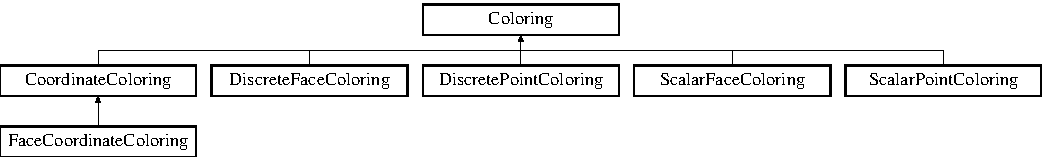
\includegraphics[height=2.113208cm]{class_coloring}
\end{center}
\end{figure}
\subsection*{Public Member Functions}
\begin{DoxyCompactItemize}
\item 
\hypertarget{class_coloring_a5502d0c484ca5f675019887da011a885}{}{\bfseries Coloring} (\hyperlink{class_shape}{Shape} $\ast$shape)\label{class_coloring_a5502d0c484ca5f675019887da011a885}

\item 
\hypertarget{class_coloring_a06fe1ecd857c9f4ccff469bec6123dd9}{}virtual void {\bfseries color} ()=0\label{class_coloring_a06fe1ecd857c9f4ccff469bec6123dd9}

\end{DoxyCompactItemize}
\subsection*{Protected Attributes}
\begin{DoxyCompactItemize}
\item 
\hypertarget{class_coloring_ae1c726b727a5a4a48cdc2999af0413d9}{}\hyperlink{class_shape}{Shape} $\ast$ {\bfseries shape\+\_\+}\label{class_coloring_ae1c726b727a5a4a48cdc2999af0413d9}

\end{DoxyCompactItemize}


The documentation for this class was generated from the following file\+:\begin{DoxyCompactItemize}
\item 
src/domain/coloring/Coloring.\+h\end{DoxyCompactItemize}

\hypertarget{class_complex_face_attribute}{}\section{Complex\+Face\+Attribute$<$ T $>$ Class Template Reference}
\label{class_complex_face_attribute}\index{Complex\+Face\+Attribute$<$ T $>$@{Complex\+Face\+Attribute$<$ T $>$}}
\subsection*{Public Member Functions}
\begin{DoxyCompactItemize}
\item 
\hypertarget{class_complex_face_attribute_a0a368d357dc8c24147ba744d7aabce89}{}{\bfseries Complex\+Face\+Attribute} (\hyperlink{class_shape}{Shape} $\ast$shape)\label{class_complex_face_attribute_a0a368d357dc8c24147ba744d7aabce89}

\item 
\hypertarget{class_complex_face_attribute_a11a16213cd62e7ada0b8a36d75043406}{}T $\ast$ {\bfseries get\+Values} ()\label{class_complex_face_attribute_a11a16213cd62e7ada0b8a36d75043406}

\item 
\hypertarget{class_complex_face_attribute_a05013475941221a1ef50b374c2c3d2d4}{}\hyperlink{class_shape}{Shape} $\ast$ {\bfseries get\+Shape} ()\label{class_complex_face_attribute_a05013475941221a1ef50b374c2c3d2d4}

\end{DoxyCompactItemize}


The documentation for this class was generated from the following file\+:\begin{DoxyCompactItemize}
\item 
src/domain/attributes/Complex\+Face\+Attribute.\+h\end{DoxyCompactItemize}

\hypertarget{class_complex_point_attribute}{}\section{Complex\+Point\+Attribute$<$ T $>$ Class Template Reference}
\label{class_complex_point_attribute}\index{Complex\+Point\+Attribute$<$ T $>$@{Complex\+Point\+Attribute$<$ T $>$}}
\subsection*{Public Member Functions}
\begin{DoxyCompactItemize}
\item 
\hypertarget{class_complex_point_attribute_adab6b6a27e00392fc6c9813a882b04c8}{}{\bfseries Complex\+Point\+Attribute} (\hyperlink{class_shape}{Shape} $\ast$shape)\label{class_complex_point_attribute_adab6b6a27e00392fc6c9813a882b04c8}

\item 
\hypertarget{class_complex_point_attribute_aaab75963a00adf77fbc0b01977e3362a}{}T $\ast$ {\bfseries get\+Values} ()\label{class_complex_point_attribute_aaab75963a00adf77fbc0b01977e3362a}

\item 
\hypertarget{class_complex_point_attribute_a4c173db22846017de47d7f0abf5cf0b7}{}\hyperlink{class_shape}{Shape} $\ast$ {\bfseries get\+Shape} ()\label{class_complex_point_attribute_a4c173db22846017de47d7f0abf5cf0b7}

\end{DoxyCompactItemize}


The documentation for this class was generated from the following file\+:\begin{DoxyCompactItemize}
\item 
src/domain/attributes/Complex\+Point\+Attribute.\+h\end{DoxyCompactItemize}

\hypertarget{class_coordinate_coloring}{}\section{Coordinate\+Coloring Class Reference}
\label{class_coordinate_coloring}\index{Coordinate\+Coloring@{Coordinate\+Coloring}}
Inheritance diagram for Coordinate\+Coloring\+:\begin{figure}[H]
\begin{center}
\leavevmode
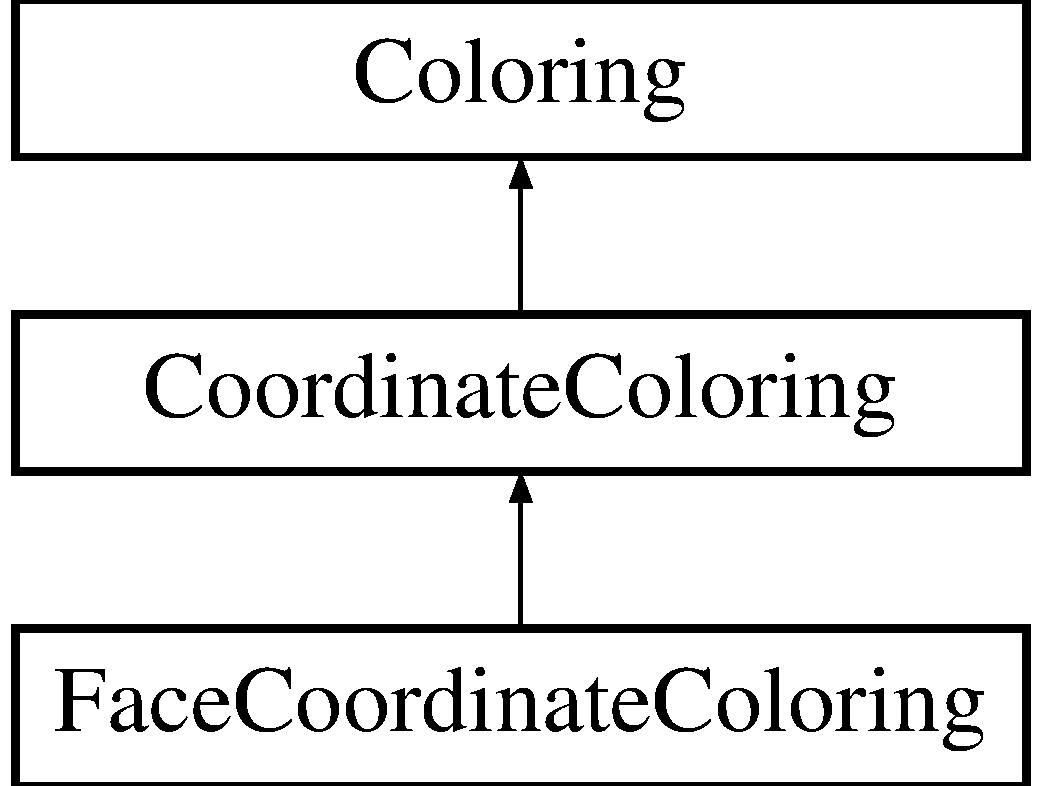
\includegraphics[height=3.000000cm]{class_coordinate_coloring}
\end{center}
\end{figure}
\subsection*{Public Member Functions}
\begin{DoxyCompactItemize}
\item 
\hypertarget{class_coordinate_coloring_ab16ae41e2bac3e484a05a95f8c3c75c8}{}{\bfseries Coordinate\+Coloring} (\hyperlink{class_shape}{Shape} $\ast$shape)\label{class_coordinate_coloring_ab16ae41e2bac3e484a05a95f8c3c75c8}

\item 
\hypertarget{class_coordinate_coloring_adfe81353e9b0791cceb013cc9a4e3f36}{}virtual void {\bfseries color} ()\label{class_coordinate_coloring_adfe81353e9b0791cceb013cc9a4e3f36}

\item 
\hypertarget{class_coordinate_coloring_acded67a88144659e774a09db49f58295}{}vtk\+Smart\+Pointer$<$ vtk\+Unsigned\+Char\+Array $>$ {\bfseries get\+Colors} ()\label{class_coordinate_coloring_acded67a88144659e774a09db49f58295}

\end{DoxyCompactItemize}
\subsection*{Additional Inherited Members}


The documentation for this class was generated from the following files\+:\begin{DoxyCompactItemize}
\item 
src/domain/coloring/Coordinate\+Coloring.\+h\item 
src/domain/coloring/Coordinate\+Coloring.\+cpp\end{DoxyCompactItemize}

\hypertarget{class_correspondence}{}\section{Correspondence Class Reference}
\label{class_correspondence}\index{Correspondence@{Correspondence}}
Inheritance diagram for Correspondence\+:\begin{figure}[H]
\begin{center}
\leavevmode
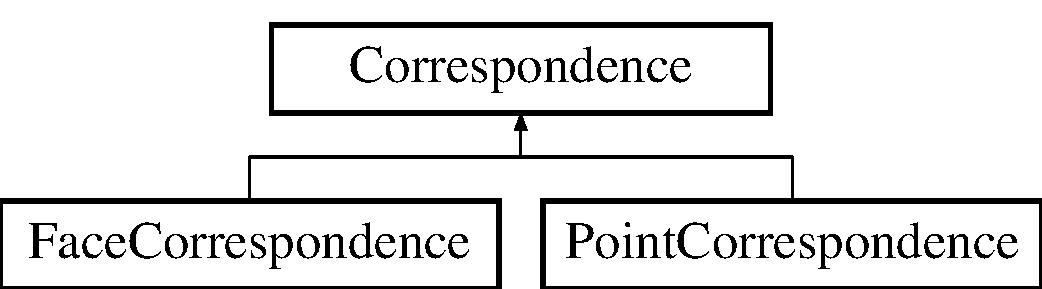
\includegraphics[height=2.000000cm]{class_correspondence}
\end{center}
\end{figure}
\subsection*{Public Member Functions}
\begin{DoxyCompactItemize}
\item 
\hypertarget{class_correspondence_a34ed80f7b9f122870e23908e08f1835f}{}void {\bfseries initialize} ()\label{class_correspondence_a34ed80f7b9f122870e23908e08f1835f}

\item 
\hypertarget{class_correspondence_aa40bb5eabdbf80573a7410bc0cf81049}{}void {\bfseries transform} (\hyperlink{class_shape}{Shape} $\ast$shape)\label{class_correspondence_aa40bb5eabdbf80573a7410bc0cf81049}

\item 
\hypertarget{class_correspondence_a7322dead4fbf4f20629c3f6c86767b99}{}void {\bfseries set\+Selected} (bool selected)\label{class_correspondence_a7322dead4fbf4f20629c3f6c86767b99}

\item 
\hypertarget{class_correspondence_a79a827237baa9ffb2bce6721177bb86c}{}int {\bfseries add\+Shape} (\hyperlink{class_shape}{Shape} $\ast$shape, vtk\+Id\+Type)\label{class_correspondence_a79a827237baa9ffb2bce6721177bb86c}

\item 
\hypertarget{class_correspondence_a180d776bd5b68d9fe79ca0b5b15dcd53}{}void {\bfseries add\+Shapes} (unordered\+\_\+map$<$ \hyperlink{class_shape}{Shape} $\ast$, vtk\+Id\+Type $>$ \&shapes)\label{class_correspondence_a180d776bd5b68d9fe79ca0b5b15dcd53}

\item 
\hypertarget{class_correspondence_ad921b2eb4bb93b90bcf1f328dfbcb5cd}{}vtk\+Actor $\ast$ {\bfseries get\+Lines\+Actor} ()\label{class_correspondence_ad921b2eb4bb93b90bcf1f328dfbcb5cd}

\item 
\hypertarget{class_correspondence_a35cc321139f0016900b27b16bf405eab}{}vector$<$ \hyperlink{class_shape}{Shape} $\ast$ $>$ \& {\bfseries get\+Shapes} ()\label{class_correspondence_a35cc321139f0016900b27b16bf405eab}

\item 
\hypertarget{class_correspondence_ad0a90dc928e29ea7bb335c3a39702439}{}\hyperlink{class_correspondence_data}{Correspondence\+Data} $\ast$ {\bfseries get\+Data} ()\label{class_correspondence_ad0a90dc928e29ea7bb335c3a39702439}

\item 
\hypertarget{class_correspondence_ae17d48fc05a5fb4a8c0e9a0d61830e48}{}void {\bfseries remove\+From\+Renderer} ()\label{class_correspondence_ae17d48fc05a5fb4a8c0e9a0d61830e48}

\item 
\hypertarget{class_correspondence_ae31e3f7d5891d44c28ac04c3bfd5b789}{}void {\bfseries add\+To\+Renderer} ()\label{class_correspondence_ae31e3f7d5891d44c28ac04c3bfd5b789}

\end{DoxyCompactItemize}
\subsection*{Protected Member Functions}
\begin{DoxyCompactItemize}
\item 
\hypertarget{class_correspondence_a321ecb3ba208f5db2d5c0f863e6cf09d}{}{\bfseries Correspondence} (vtk\+Smart\+Pointer$<$ vtk\+Renderer $>$ renderer, \hyperlink{class_correspondence_data}{Correspondence\+Data} $\ast$data)\label{class_correspondence_a321ecb3ba208f5db2d5c0f863e6cf09d}

\item 
\hypertarget{class_correspondence_af488f3525bddc4f637ac8696d59d72af}{}{\bfseries Correspondence} (vtk\+Smart\+Pointer$<$ vtk\+Renderer $>$ renderer, \hyperlink{class_correspondence_data}{Correspondence\+Data} $\ast$data, \hyperlink{class_hash_map}{Hash\+Map}$<$ vtk\+Actor $\ast$, \hyperlink{class_shape}{Shape} $\ast$ $>$ \&shapes)\label{class_correspondence_af488f3525bddc4f637ac8696d59d72af}

\item 
\hypertarget{class_correspondence_a98e73443c89db8acd848db19a40f7978}{}virtual void {\bfseries initialize\+Actor} (vtk\+Smart\+Pointer$<$ vtk\+Actor $>$ actor, \hyperlink{class_shape}{Shape} $\ast$shape, vtk\+Id\+Type)=0\label{class_correspondence_a98e73443c89db8acd848db19a40f7978}

\item 
\hypertarget{class_correspondence_a0253e13319957d2547b69196d07ad3ea}{}virtual void {\bfseries get\+Correspondence\+Point} (double point\mbox{[}3\mbox{]}, \hyperlink{class_shape}{Shape} $\ast$shape, vtk\+Id\+Type)=0\label{class_correspondence_a0253e13319957d2547b69196d07ad3ea}

\end{DoxyCompactItemize}
\subsection*{Protected Attributes}
\begin{DoxyCompactItemize}
\item 
\hypertarget{class_correspondence_a872cd57c92e18a1af86793d8a0e29dae}{}vtk\+Smart\+Pointer$<$ vtk\+Renderer $>$ {\bfseries renderer\+\_\+}\label{class_correspondence_a872cd57c92e18a1af86793d8a0e29dae}

\item 
\hypertarget{class_correspondence_aa82f3556aebfd19e7fdcedd5338fd7c2}{}\hyperlink{class_correspondence_data}{Correspondence\+Data} $\ast$ {\bfseries data\+\_\+}\label{class_correspondence_aa82f3556aebfd19e7fdcedd5338fd7c2}

\item 
\hypertarget{class_correspondence_a209aad8fcf25d57cf5497c0e412a17a8}{}vector$<$ \hyperlink{class_shape}{Shape} $\ast$ $>$ {\bfseries shapes\+\_\+}\label{class_correspondence_a209aad8fcf25d57cf5497c0e412a17a8}

\item 
\hypertarget{class_correspondence_aee809c04f1f97da83f4ee6059b1a91bf}{}vector$<$ vtk\+Smart\+Pointer$<$ vtk\+Actor $>$ $>$ {\bfseries actors\+\_\+}\label{class_correspondence_aee809c04f1f97da83f4ee6059b1a91bf}

\item 
\hypertarget{class_correspondence_ad4330bf4a1bb84fbe67e2563c8baa8c3}{}vtk\+Smart\+Pointer$<$ vtk\+Points $>$ {\bfseries line\+Reference\+Points\+\_\+}\label{class_correspondence_ad4330bf4a1bb84fbe67e2563c8baa8c3}

\item 
\hypertarget{class_correspondence_aca2749697165656c651cf41b5208b7fa}{}vtk\+Smart\+Pointer$<$ vtk\+Poly\+Data $>$ {\bfseries lines\+Poly\+Data\+\_\+}\label{class_correspondence_aca2749697165656c651cf41b5208b7fa}

\item 
\hypertarget{class_correspondence_af77759b08266d787154b30a36c24b33a}{}vtk\+Smart\+Pointer$<$ vtk\+Poly\+Data\+Mapper $>$ {\bfseries lines\+Mapper\+\_\+}\label{class_correspondence_af77759b08266d787154b30a36c24b33a}

\item 
\hypertarget{class_correspondence_a7950b1784f8318a085c5f7d126bd1984}{}vtk\+Smart\+Pointer$<$ vtk\+Actor $>$ {\bfseries lines\+Actor\+\_\+}\label{class_correspondence_a7950b1784f8318a085c5f7d126bd1984}

\end{DoxyCompactItemize}


The documentation for this class was generated from the following files\+:\begin{DoxyCompactItemize}
\item 
src/domain/correspondences/Correspondence.\+h\item 
src/domain/correspondences/Correspondence.\+cpp\end{DoxyCompactItemize}

\hypertarget{class_correspondence_coloring}{}\section{Correspondence\+Coloring Class Reference}
\label{class_correspondence_coloring}\index{Correspondence\+Coloring@{Correspondence\+Coloring}}
\subsection*{Public Member Functions}
\begin{DoxyCompactItemize}
\item 
\hypertarget{class_correspondence_coloring_a1b933996e280406cc77f48c07e9c6dc7}{}{\bfseries Correspondence\+Coloring} (\hyperlink{class_hash_map}{Hash\+Map}$<$ vtk\+Actor $\ast$, \hyperlink{class_shape}{Shape} $\ast$ $>$ $\ast$set, \hyperlink{class_hash_map}{Hash\+Map}$<$ \hyperlink{class_point_correspondence_data}{Point\+Correspondence\+Data} $\ast$, bool $>$ $\ast$points, \hyperlink{class_hash_map}{Hash\+Map}$<$ \hyperlink{class_face_correspondence_data}{Face\+Correspondence\+Data} $\ast$, bool $>$ $\ast$faces, \hyperlink{class_shape}{Shape} $\ast$reference=0)\label{class_correspondence_coloring_a1b933996e280406cc77f48c07e9c6dc7}

\item 
\hypertarget{class_correspondence_coloring_a664467e021d1b49a693218ae56728537}{}void {\bfseries show\+Point\+Correspondences} (vector$<$ pair$<$ vtk\+Id\+Type, double $>$ $>$ $\ast$percentage\+Matched=0, vector$<$ pair$<$ vtk\+Id\+Type, double $>$ $>$ $\ast$percentage\+Multiple=0)\label{class_correspondence_coloring_a664467e021d1b49a693218ae56728537}

\item 
\hypertarget{class_correspondence_coloring_a01d90e7657d270d3420773f79ad6dbca}{}void {\bfseries show\+Face\+Correspondences} (vector$<$ pair$<$ vtk\+Id\+Type, double $>$ $>$ $\ast$percentage\+Matched=0, vector$<$ pair$<$ vtk\+Id\+Type, double $>$ $>$ $\ast$percentage\+Multiple=0)\label{class_correspondence_coloring_a01d90e7657d270d3420773f79ad6dbca}

\end{DoxyCompactItemize}
\subsection*{Protected Attributes}
\begin{DoxyCompactItemize}
\item 
\hypertarget{class_correspondence_coloring_a279562196a4636d10f1d54319eb96129}{}\hyperlink{class_hash_map}{Hash\+Map}$<$ vtk\+Actor $\ast$, \hyperlink{class_shape}{Shape} $\ast$ $>$ $\ast$ {\bfseries shapes\+\_\+}\label{class_correspondence_coloring_a279562196a4636d10f1d54319eb96129}

\item 
\hypertarget{class_correspondence_coloring_a925be65ac98dabc0959085f7972c79f1}{}\hyperlink{class_hash_map}{Hash\+Map}$<$ \hyperlink{class_point_correspondence_data}{Point\+Correspondence\+Data} $\ast$, bool $>$ $\ast$ {\bfseries points\+\_\+}\label{class_correspondence_coloring_a925be65ac98dabc0959085f7972c79f1}

\item 
\hypertarget{class_correspondence_coloring_a61ef00707cd1882293d58cfb750ab2f2}{}\hyperlink{class_hash_map}{Hash\+Map}$<$ \hyperlink{class_face_correspondence_data}{Face\+Correspondence\+Data} $\ast$, bool $>$ $\ast$ {\bfseries faces\+\_\+}\label{class_correspondence_coloring_a61ef00707cd1882293d58cfb750ab2f2}

\item 
\hypertarget{class_correspondence_coloring_a30cb4c9172b8edf1a0597fed5e0270a0}{}\hyperlink{class_shape}{Shape} $\ast$ {\bfseries reference\+\_\+}\label{class_correspondence_coloring_a30cb4c9172b8edf1a0597fed5e0270a0}

\item 
\hypertarget{class_correspondence_coloring_ab9fddd8872a1af4208c4622691e5dbaf}{}unordered\+\_\+map$<$ vtk\+Id\+Type, vtk\+Smart\+Pointer$<$ vtk\+Unsigned\+Char\+Array $>$ $>$ {\bfseries point\+Attributes\+\_\+}\label{class_correspondence_coloring_ab9fddd8872a1af4208c4622691e5dbaf}

\item 
\hypertarget{class_correspondence_coloring_a964a931d8747f1c8c85e28c0f0ff8e48}{}unordered\+\_\+map$<$ vtk\+Id\+Type, vtk\+Smart\+Pointer$<$ vtk\+Unsigned\+Char\+Array $>$ $>$ {\bfseries face\+Attributes\+\_\+}\label{class_correspondence_coloring_a964a931d8747f1c8c85e28c0f0ff8e48}

\end{DoxyCompactItemize}


The documentation for this class was generated from the following files\+:\begin{DoxyCompactItemize}
\item 
src/domain/coloring/Correspondence\+Coloring.\+h\item 
src/domain/coloring/Correspondence\+Coloring.\+cpp\end{DoxyCompactItemize}

\hypertarget{class_ui_1_1_correspondence_coloring_widget}{}\section{Ui\+:\+:Correspondence\+Coloring\+Widget Class Reference}
\label{class_ui_1_1_correspondence_coloring_widget}\index{Ui\+::\+Correspondence\+Coloring\+Widget@{Ui\+::\+Correspondence\+Coloring\+Widget}}
Inheritance diagram for Ui\+:\+:Correspondence\+Coloring\+Widget\+:\begin{figure}[H]
\begin{center}
\leavevmode
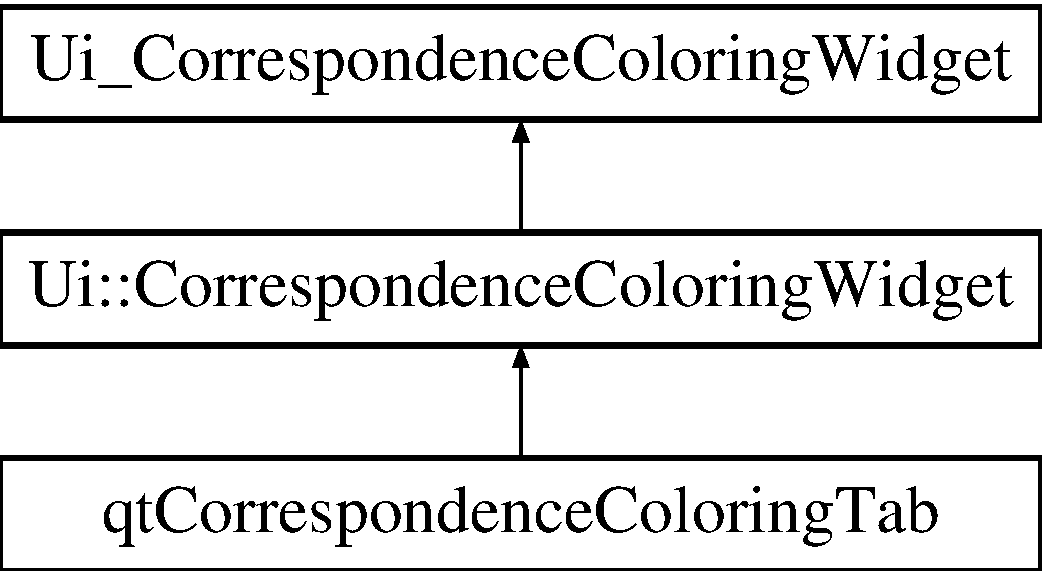
\includegraphics[height=3.000000cm]{class_ui_1_1_correspondence_coloring_widget}
\end{center}
\end{figure}
\subsection*{Additional Inherited Members}


The documentation for this class was generated from the following file\+:\begin{DoxyCompactItemize}
\item 
build/ui\+\_\+correspondence\+Coloring.\+h\end{DoxyCompactItemize}

\hypertarget{class_correspondence_data}{}\section{Correspondence\+Data Class Reference}
\label{class_correspondence_data}\index{Correspondence\+Data@{Correspondence\+Data}}
Inheritance diagram for Correspondence\+Data\+:\begin{figure}[H]
\begin{center}
\leavevmode
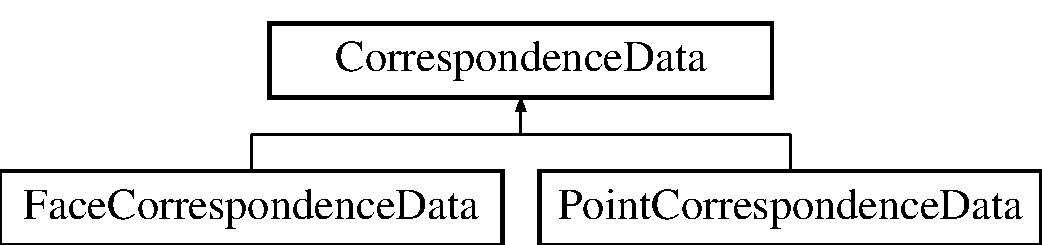
\includegraphics[height=2.000000cm]{class_correspondence_data}
\end{center}
\end{figure}
\subsection*{Public Member Functions}
\begin{DoxyCompactItemize}
\item 
\hypertarget{class_correspondence_data_abdf278997d70f654647ab521589733f8}{}void {\bfseries add\+Shape} (const vtk\+Id\+Type new\+Shape, const vtk\+Id\+Type new\+Correspondence)\label{class_correspondence_data_abdf278997d70f654647ab521589733f8}

\item 
\hypertarget{class_correspondence_data_a4bce18620695e23262206e7e1f8a860f}{}void {\bfseries clear} ()\label{class_correspondence_data_a4bce18620695e23262206e7e1f8a860f}

\item 
\hypertarget{class_correspondence_data_a094039b5f79ff82898d7a940b98203fe}{}vector$<$ vtk\+Id\+Type $>$ \& {\bfseries get\+Shape\+Ids} ()\label{class_correspondence_data_a094039b5f79ff82898d7a940b98203fe}

\item 
\hypertarget{class_correspondence_data_a8b5c45708c2ca5e7a8671de9a7f9f635}{}vector$<$ vtk\+Id\+Type $>$ \& {\bfseries get\+Corresponding\+Ids} ()\label{class_correspondence_data_a8b5c45708c2ca5e7a8671de9a7f9f635}

\item 
\hypertarget{class_correspondence_data_ad6746b995840c277e0a0b2c0ae0afe81}{}int {\bfseries size} ()\label{class_correspondence_data_ad6746b995840c277e0a0b2c0ae0afe81}

\item 
\hypertarget{class_correspondence_data_a990fb28e8aa665c9aa7c77b17b1ba64c}{}vtk\+Id\+Type {\bfseries get\+Id} ()\label{class_correspondence_data_a990fb28e8aa665c9aa7c77b17b1ba64c}

\item 
\hypertarget{class_correspondence_data_ab374d531599a7bf59e262191263dc147}{}string {\bfseries to\+String} ()\label{class_correspondence_data_ab374d531599a7bf59e262191263dc147}

\item 
\hypertarget{class_correspondence_data_a060f3788975ef1c3129114f191c41650}{}virtual string {\bfseries get\+Type} ()=0\label{class_correspondence_data_a060f3788975ef1c3129114f191c41650}

\end{DoxyCompactItemize}
\subsection*{Protected Member Functions}
\begin{DoxyCompactItemize}
\item 
\hypertarget{class_correspondence_data_a07e83374f490dc9039396a31561bd32a}{}{\bfseries Correspondence\+Data} (vtk\+Id\+Type id)\label{class_correspondence_data_a07e83374f490dc9039396a31561bd32a}

\end{DoxyCompactItemize}
\subsection*{Protected Attributes}
\begin{DoxyCompactItemize}
\item 
\hypertarget{class_correspondence_data_a9d064aa6c9252072cdf8537929261dad}{}vector$<$ vtk\+Id\+Type $>$ {\bfseries shape\+Ids\+\_\+}\label{class_correspondence_data_a9d064aa6c9252072cdf8537929261dad}

\item 
\hypertarget{class_correspondence_data_a5a4e8a0ecbbf3a029a7b453407b363f8}{}vector$<$ vtk\+Id\+Type $>$ {\bfseries corresponding\+Ids\+\_\+}\label{class_correspondence_data_a5a4e8a0ecbbf3a029a7b453407b363f8}

\item 
\hypertarget{class_correspondence_data_a5f5964ac0e1e46f9010dcef28f42bd35}{}vtk\+Id\+Type {\bfseries id\+\_\+}\label{class_correspondence_data_a5f5964ac0e1e46f9010dcef28f42bd35}

\end{DoxyCompactItemize}


The documentation for this class was generated from the following file\+:\begin{DoxyCompactItemize}
\item 
src/domain/correspondences/Correspondence\+Data.\+h\end{DoxyCompactItemize}

\hypertarget{class_correspondence_picker}{}\section{Correspondence\+Picker Class Reference}
\label{class_correspondence_picker}\index{Correspondence\+Picker@{Correspondence\+Picker}}
Inheritance diagram for Correspondence\+Picker\+:\begin{figure}[H]
\begin{center}
\leavevmode

\includegraphics[height=2.000000cm]{class_correspondence_picker}
\end{center}
\end{figure}
\subsection*{Public Member Functions}
\begin{DoxyCompactItemize}
\item 
\hypertarget{class_correspondence_picker_adac4887aba7012e30460bec9774ecda3}{}int {\bfseries add\+Shape} (\hyperlink{class_shape}{Shape} $\ast$shape, vtk\+Id\+Type selection\+Id)\label{class_correspondence_picker_adac4887aba7012e30460bec9774ecda3}

\item 
\hypertarget{class_correspondence_picker_aa0d44137c5312b42138b6a16c795fe4f}{}bool {\bfseries pick} (\hyperlink{class_correspondence}{Correspondence} $\ast$$\ast$correspondence)\label{class_correspondence_picker_aa0d44137c5312b42138b6a16c795fe4f}

\item 
\hypertarget{class_correspondence_picker_a29a99b7b5adfb4c2514b1a67de5a877e}{}void {\bfseries update\+Mouse\+Line} (int x, int y)\label{class_correspondence_picker_a29a99b7b5adfb4c2514b1a67de5a877e}

\item 
\hypertarget{class_correspondence_picker_a2394504b680fc8344c26e57e899f08a9}{}void {\bfseries clear\+Selection} ()\label{class_correspondence_picker_a2394504b680fc8344c26e57e899f08a9}

\end{DoxyCompactItemize}
\subsection*{Protected Member Functions}
\begin{DoxyCompactItemize}
\item 
\hypertarget{class_correspondence_picker_a70285e89add0a5df7596bdddc0f132b7}{}{\bfseries Correspondence\+Picker} (vtk\+Renderer $\ast$renderer, int \&last\+Insert\+Correspondence\+I\+D)\label{class_correspondence_picker_a70285e89add0a5df7596bdddc0f132b7}

\item 
\hypertarget{class_correspondence_picker_a14b40e8ee44c95e360d6f7665267c6df}{}virtual void {\bfseries get\+Current\+Selection\+Point} (\hyperlink{class_shape}{Shape} $\ast$shape, vtk\+Id\+Type, double point\mbox{[}3\mbox{]})=0\label{class_correspondence_picker_a14b40e8ee44c95e360d6f7665267c6df}

\item 
\hypertarget{class_correspondence_picker_ac6d3217637060205e72e6ae19096f812}{}virtual void {\bfseries visualize\+Current\+Selection} (\hyperlink{class_shape}{Shape} $\ast$shape, vtk\+Id\+Type)=0\label{class_correspondence_picker_ac6d3217637060205e72e6ae19096f812}

\item 
\hypertarget{class_correspondence_picker_a2470d78722d9d164323cd820aa9f572a}{}virtual \hyperlink{class_correspondence}{Correspondence} $\ast$ {\bfseries create\+Correspondence} ()=0\label{class_correspondence_picker_a2470d78722d9d164323cd820aa9f572a}

\end{DoxyCompactItemize}
\subsection*{Protected Attributes}
\begin{DoxyCompactItemize}
\item 
\hypertarget{class_correspondence_picker_a6fecd46b5c6eb12d55cf62b4dbdf8b1f}{}vtk\+Smart\+Pointer$<$ vtk\+Actor $>$ {\bfseries current\+Selection\+Actor\+\_\+}\label{class_correspondence_picker_a6fecd46b5c6eb12d55cf62b4dbdf8b1f}

\item 
\hypertarget{class_correspondence_picker_a3e59d81ec22903c96d330d0c3aee16e4}{}vtk\+Smart\+Pointer$<$ vtk\+Poly\+Data\+Mapper $>$ {\bfseries current\+Selection\+Mapper\+\_\+}\label{class_correspondence_picker_a3e59d81ec22903c96d330d0c3aee16e4}

\item 
\hypertarget{class_correspondence_picker_aac2fd778113fa0b6a0668a0ffd83ab86}{}vtk\+Renderer $\ast$ {\bfseries renderer\+\_\+}\label{class_correspondence_picker_aac2fd778113fa0b6a0668a0ffd83ab86}

\item 
\hypertarget{class_correspondence_picker_adae7b5e7bb605c1e93753bf4e42beadd}{}int \& {\bfseries last\+Insert\+Correspondence\+I\+D\+\_\+}\label{class_correspondence_picker_adae7b5e7bb605c1e93753bf4e42beadd}

\end{DoxyCompactItemize}


The documentation for this class was generated from the following files\+:\begin{DoxyCompactItemize}
\item 
src/view/Correspondence\+Picker.\+h\item 
src/view/Correspondence\+Picker.\+cpp\end{DoxyCompactItemize}

\hypertarget{class_ui_1_1_dialog}{}\section{Ui\+:\+:Dialog Class Reference}
\label{class_ui_1_1_dialog}\index{Ui\+::\+Dialog@{Ui\+::\+Dialog}}
Inheritance diagram for Ui\+:\+:Dialog\+:\begin{figure}[H]
\begin{center}
\leavevmode
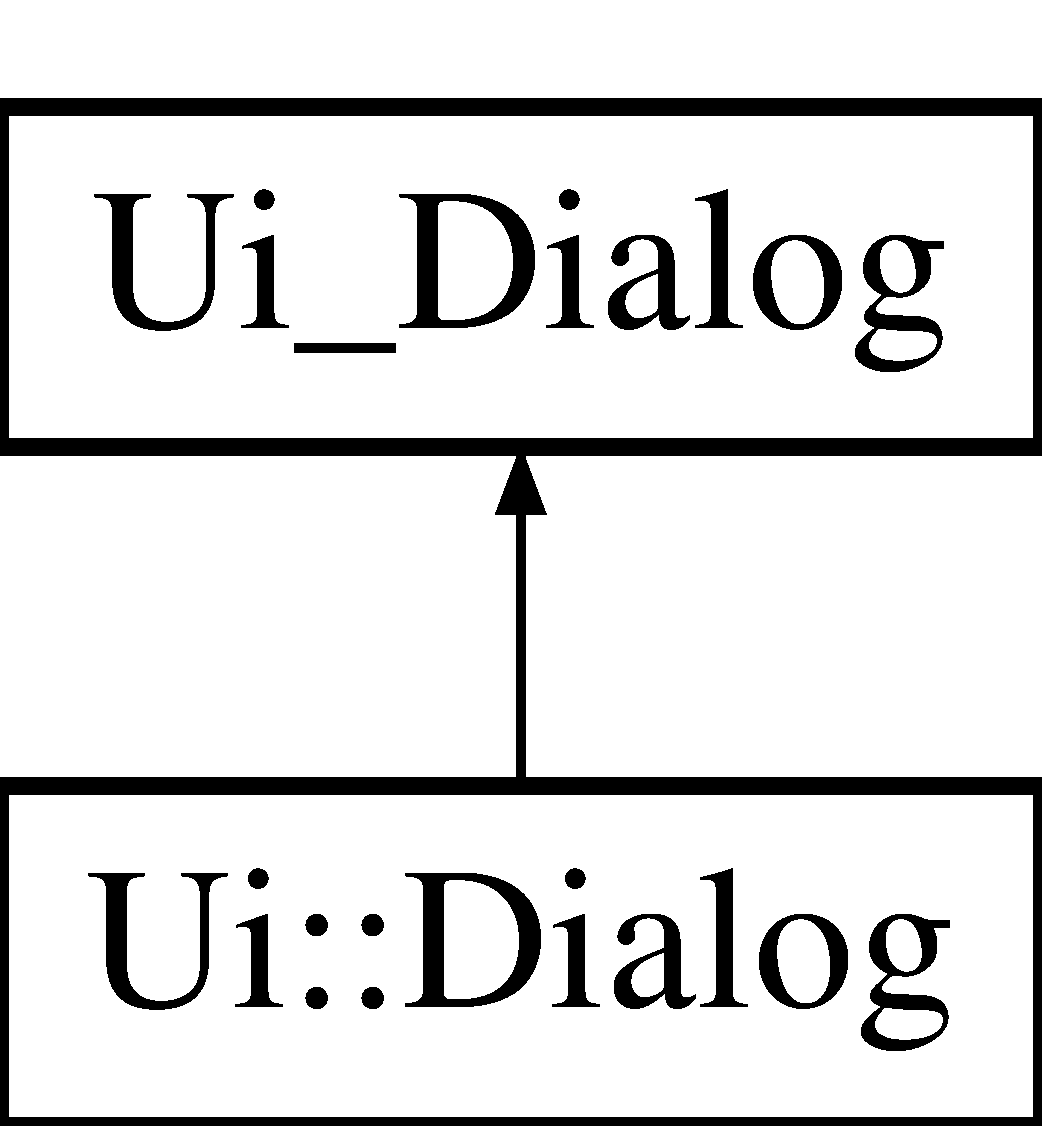
\includegraphics[height=2.000000cm]{class_ui_1_1_dialog}
\end{center}
\end{figure}
\subsection*{Additional Inherited Members}


The documentation for this class was generated from the following file\+:\begin{DoxyCompactItemize}
\item 
build/ui\+\_\+help.\+h\end{DoxyCompactItemize}

\hypertarget{classgeodesic_1_1_dijkstra_node}{}\section{geodesic\+:\+:Dijkstra\+Node Class Reference}
\label{classgeodesic_1_1_dijkstra_node}\index{geodesic\+::\+Dijkstra\+Node@{geodesic\+::\+Dijkstra\+Node}}
\subsection*{Public Member Functions}
\begin{DoxyCompactItemize}
\item 
\hypertarget{classgeodesic_1_1_dijkstra_node_a99d02fd851e23c492aa1eeff4f67a7d7}{}double \& {\bfseries distance\+\_\+from\+\_\+source} ()\label{classgeodesic_1_1_dijkstra_node_a99d02fd851e23c492aa1eeff4f67a7d7}

\item 
\hypertarget{classgeodesic_1_1_dijkstra_node_a4c1a78e5803d668edd78af52388844ad}{}\hyperlink{classgeodesic_1_1_dijkstra_node}{node\+\_\+pointer} \& {\bfseries previous} ()\label{classgeodesic_1_1_dijkstra_node_a4c1a78e5803d668edd78af52388844ad}

\item 
\hypertarget{classgeodesic_1_1_dijkstra_node_afd2f3fc288efa56371142da3f3d40161}{}unsigned \& {\bfseries source\+\_\+index} ()\label{classgeodesic_1_1_dijkstra_node_afd2f3fc288efa56371142da3f3d40161}

\item 
\hypertarget{classgeodesic_1_1_dijkstra_node_ad305dc92e8fb46bb7309473bffc29f80}{}\hyperlink{classgeodesic_1_1_vertex}{vertex\+\_\+pointer} \& {\bfseries vertex} ()\label{classgeodesic_1_1_dijkstra_node_ad305dc92e8fb46bb7309473bffc29f80}

\item 
\hypertarget{classgeodesic_1_1_dijkstra_node_ab8c56944371a9da0e9532e8cc8e7e153}{}void {\bfseries clear} ()\label{classgeodesic_1_1_dijkstra_node_ab8c56944371a9da0e9532e8cc8e7e153}

\item 
\hypertarget{classgeodesic_1_1_dijkstra_node_a8ff6eb08aacd8a75b509ea2a3640b99d}{}bool {\bfseries operator()} (\hyperlink{classgeodesic_1_1_dijkstra_node}{node\+\_\+pointer} const s1, \hyperlink{classgeodesic_1_1_dijkstra_node}{node\+\_\+pointer} const s2) const \label{classgeodesic_1_1_dijkstra_node_a8ff6eb08aacd8a75b509ea2a3640b99d}

\item 
\hypertarget{classgeodesic_1_1_dijkstra_node_aa21bf0c4f5b858731ef2103663728c37}{}double {\bfseries distance} (\hyperlink{classgeodesic_1_1_surface_point}{Surface\+Point} $\ast$p)\label{classgeodesic_1_1_dijkstra_node_aa21bf0c4f5b858731ef2103663728c37}

\item 
\hypertarget{classgeodesic_1_1_dijkstra_node_a0376f6231c4b485561418cff249939b4}{}\hyperlink{classgeodesic_1_1_surface_point}{Surface\+Point} {\bfseries surface\+\_\+point} ()\label{classgeodesic_1_1_dijkstra_node_a0376f6231c4b485561418cff249939b4}

\end{DoxyCompactItemize}


The documentation for this class was generated from the following file\+:\begin{DoxyCompactItemize}
\item 
src/domain/metric/3rdparty/geodesic/geodesic\+\_\+algorithm\+\_\+dijkstra.\+h\end{DoxyCompactItemize}

\hypertarget{classgeodesic_1_1_dijkstra_node1}{}\section{geodesic\+:\+:Dijkstra\+Node1 Class Reference}
\label{classgeodesic_1_1_dijkstra_node1}\index{geodesic\+::\+Dijkstra\+Node1@{geodesic\+::\+Dijkstra\+Node1}}
\subsection*{Public Member Functions}
\begin{DoxyCompactItemize}
\item 
\hypertarget{classgeodesic_1_1_dijkstra_node1_a4319ff7c12733f0d79aa119ddbd1bcdd}{}double \& {\bfseries distance\+\_\+from\+\_\+source} ()\label{classgeodesic_1_1_dijkstra_node1_a4319ff7c12733f0d79aa119ddbd1bcdd}

\item 
\hypertarget{classgeodesic_1_1_dijkstra_node1_abe89a88d7514fbad05b2ab66d995d8b0}{}\hyperlink{classgeodesic_1_1_dijkstra_node1}{node\+\_\+pointer} \& {\bfseries previous} ()\label{classgeodesic_1_1_dijkstra_node1_abe89a88d7514fbad05b2ab66d995d8b0}

\item 
\hypertarget{classgeodesic_1_1_dijkstra_node1_ac44a2aa7b48823d59145e240447ff1f5}{}unsigned \& {\bfseries source\+\_\+index} ()\label{classgeodesic_1_1_dijkstra_node1_ac44a2aa7b48823d59145e240447ff1f5}

\item 
\hypertarget{classgeodesic_1_1_dijkstra_node1_a88ef4f97b8e7070b07029c61d7e96904}{}\hyperlink{classgeodesic_1_1_vertex}{vertex\+\_\+pointer} \& {\bfseries vertex} ()\label{classgeodesic_1_1_dijkstra_node1_a88ef4f97b8e7070b07029c61d7e96904}

\item 
\hypertarget{classgeodesic_1_1_dijkstra_node1_ae6e22cf8c828285fbc89f149e3126b9c}{}void {\bfseries clear} ()\label{classgeodesic_1_1_dijkstra_node1_ae6e22cf8c828285fbc89f149e3126b9c}

\item 
\hypertarget{classgeodesic_1_1_dijkstra_node1_a0762ca782bc52cdb4346d937fee228de}{}bool {\bfseries operator()} (\hyperlink{classgeodesic_1_1_dijkstra_node1}{node\+\_\+pointer} const s1, \hyperlink{classgeodesic_1_1_dijkstra_node1}{node\+\_\+pointer} const s2) const \label{classgeodesic_1_1_dijkstra_node1_a0762ca782bc52cdb4346d937fee228de}

\end{DoxyCompactItemize}


The documentation for this class was generated from the following file\+:\begin{DoxyCompactItemize}
\item 
src/domain/metric/3rdparty/geodesic/geodesic\+\_\+algorithm\+\_\+dijkstra\+\_\+alternative.\+h\end{DoxyCompactItemize}

\hypertarget{class_discrete_face_attribute}{}\section{Discrete\+Face\+Attribute Class Reference}
\label{class_discrete_face_attribute}\index{Discrete\+Face\+Attribute@{Discrete\+Face\+Attribute}}
\subsection*{Public Member Functions}
\begin{DoxyCompactItemize}
\item 
\hypertarget{class_discrete_face_attribute_ad7183266e3e7d927f2b53ffe4dace110}{}{\bfseries Discrete\+Face\+Attribute} (\hyperlink{class_shape}{Shape} $\ast$shape)\label{class_discrete_face_attribute_ad7183266e3e7d927f2b53ffe4dace110}

\item 
\hypertarget{class_discrete_face_attribute_a9767d19deae2768b95f06499cd6a4bda}{}vtk\+Smart\+Pointer$<$ vtk\+Int\+Array $>$ {\bfseries get\+Values} ()\label{class_discrete_face_attribute_a9767d19deae2768b95f06499cd6a4bda}

\item 
\hypertarget{class_discrete_face_attribute_ac2411ea78be1cc03ef7cd003c802711d}{}\hyperlink{class_shape}{Shape} $\ast$ {\bfseries get\+Shape} ()\label{class_discrete_face_attribute_ac2411ea78be1cc03ef7cd003c802711d}

\end{DoxyCompactItemize}


The documentation for this class was generated from the following files\+:\begin{DoxyCompactItemize}
\item 
src/domain/attributes/Discrete\+Face\+Attribute.\+h\item 
src/domain/attributes/Discrete\+Face\+Attribute.\+cpp\end{DoxyCompactItemize}

\hypertarget{class_discrete_face_coloring}{}\section{Discrete\+Face\+Coloring Class Reference}
\label{class_discrete_face_coloring}\index{Discrete\+Face\+Coloring@{Discrete\+Face\+Coloring}}
Inheritance diagram for Discrete\+Face\+Coloring\+:\begin{figure}[H]
\begin{center}
\leavevmode
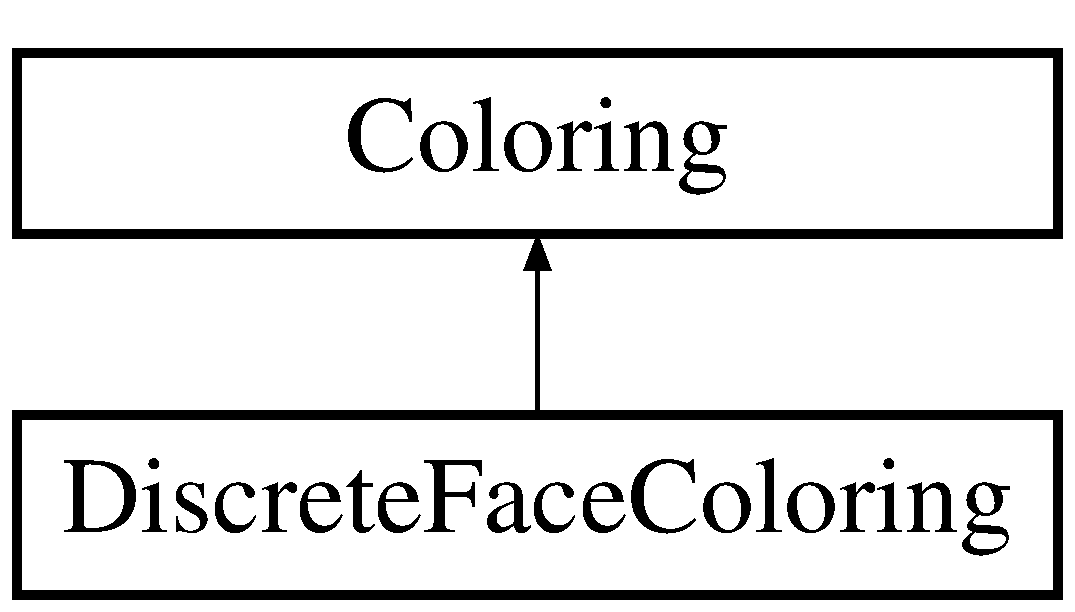
\includegraphics[height=2.000000cm]{class_discrete_face_coloring}
\end{center}
\end{figure}
\subsection*{Public Member Functions}
\begin{DoxyCompactItemize}
\item 
\hypertarget{class_discrete_face_coloring_a28b50f0c89173d067489e42fb36373e8}{}{\bfseries Discrete\+Face\+Coloring} (\hyperlink{class_shape}{Shape} $\ast$shape, \hyperlink{class_discrete_face_attribute}{Discrete\+Face\+Attribute} \&attribute)\label{class_discrete_face_coloring_a28b50f0c89173d067489e42fb36373e8}

\item 
\hypertarget{class_discrete_face_coloring_a9949374e0af166fdc322475971e9d612}{}virtual void {\bfseries color} ()\label{class_discrete_face_coloring_a9949374e0af166fdc322475971e9d612}

\end{DoxyCompactItemize}
\subsection*{Protected Attributes}
\begin{DoxyCompactItemize}
\item 
\hypertarget{class_discrete_face_coloring_a665f2316ca228e8c281b5b77eb7196e9}{}\hyperlink{class_discrete_face_attribute}{Discrete\+Face\+Attribute} \& {\bfseries attribute\+\_\+}\label{class_discrete_face_coloring_a665f2316ca228e8c281b5b77eb7196e9}

\end{DoxyCompactItemize}


The documentation for this class was generated from the following files\+:\begin{DoxyCompactItemize}
\item 
src/domain/coloring/Discrete\+Face\+Coloring.\+h\item 
src/domain/coloring/Discrete\+Face\+Coloring.\+cpp\end{DoxyCompactItemize}

\hypertarget{class_discrete_point_attribute}{}\section{Discrete\+Point\+Attribute Class Reference}
\label{class_discrete_point_attribute}\index{Discrete\+Point\+Attribute@{Discrete\+Point\+Attribute}}
\subsection*{Public Member Functions}
\begin{DoxyCompactItemize}
\item 
\hypertarget{class_discrete_point_attribute_ae621f748d818a634a3048cb4a91722fa}{}{\bfseries Discrete\+Point\+Attribute} (\hyperlink{class_shape}{Shape} $\ast$shape)\label{class_discrete_point_attribute_ae621f748d818a634a3048cb4a91722fa}

\item 
\hypertarget{class_discrete_point_attribute_a0516593a4f91658c1cbee796c700ca2e}{}vtk\+Smart\+Pointer$<$ vtk\+Int\+Array $>$ {\bfseries get\+Values} ()\label{class_discrete_point_attribute_a0516593a4f91658c1cbee796c700ca2e}

\item 
\hypertarget{class_discrete_point_attribute_a5b75b8aa4b8c0ad8b6b1752b15451337}{}\hyperlink{class_shape}{Shape} $\ast$ {\bfseries get\+Shape} ()\label{class_discrete_point_attribute_a5b75b8aa4b8c0ad8b6b1752b15451337}

\end{DoxyCompactItemize}


The documentation for this class was generated from the following files\+:\begin{DoxyCompactItemize}
\item 
src/domain/attributes/Discrete\+Point\+Attribute.\+h\item 
src/domain/attributes/Discrete\+Point\+Attribute.\+cpp\end{DoxyCompactItemize}

\hypertarget{class_discrete_point_coloring}{}\section{Discrete\+Point\+Coloring Class Reference}
\label{class_discrete_point_coloring}\index{Discrete\+Point\+Coloring@{Discrete\+Point\+Coloring}}
Inheritance diagram for Discrete\+Point\+Coloring\+:\begin{figure}[H]
\begin{center}
\leavevmode
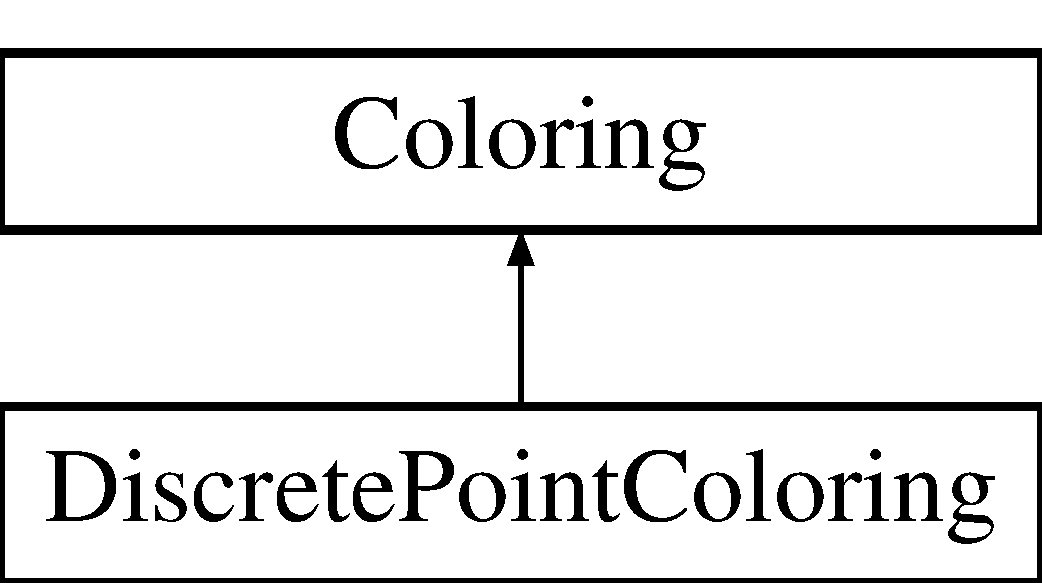
\includegraphics[height=2.000000cm]{class_discrete_point_coloring}
\end{center}
\end{figure}
\subsection*{Public Member Functions}
\begin{DoxyCompactItemize}
\item 
\hypertarget{class_discrete_point_coloring_a3d112ea40b0775466b85479931c3d6fa}{}{\bfseries Discrete\+Point\+Coloring} (\hyperlink{class_shape}{Shape} $\ast$shape, \hyperlink{class_discrete_point_attribute}{Discrete\+Point\+Attribute} \&attribute)\label{class_discrete_point_coloring_a3d112ea40b0775466b85479931c3d6fa}

\item 
\hypertarget{class_discrete_point_coloring_acbc9d6aee4a0fb0e3994d3ca41a459a1}{}virtual void {\bfseries color} ()\label{class_discrete_point_coloring_acbc9d6aee4a0fb0e3994d3ca41a459a1}

\end{DoxyCompactItemize}
\subsection*{Protected Attributes}
\begin{DoxyCompactItemize}
\item 
\hypertarget{class_discrete_point_coloring_a560fb18a73bd3ca0da2b44b5ab66ef8a}{}\hyperlink{class_discrete_point_attribute}{Discrete\+Point\+Attribute} \& {\bfseries attribute\+\_\+}\label{class_discrete_point_coloring_a560fb18a73bd3ca0da2b44b5ab66ef8a}

\end{DoxyCompactItemize}


The documentation for this class was generated from the following files\+:\begin{DoxyCompactItemize}
\item 
src/domain/coloring/Discrete\+Point\+Coloring.\+h\item 
src/domain/coloring/Discrete\+Point\+Coloring.\+cpp\end{DoxyCompactItemize}

\hypertarget{classgeodesic_1_1_edge}{}\section{geodesic\+:\+:Edge Class Reference}
\label{classgeodesic_1_1_edge}\index{geodesic\+::\+Edge@{geodesic\+::\+Edge}}
Inheritance diagram for geodesic\+:\+:Edge\+:\begin{figure}[H]
\begin{center}
\leavevmode
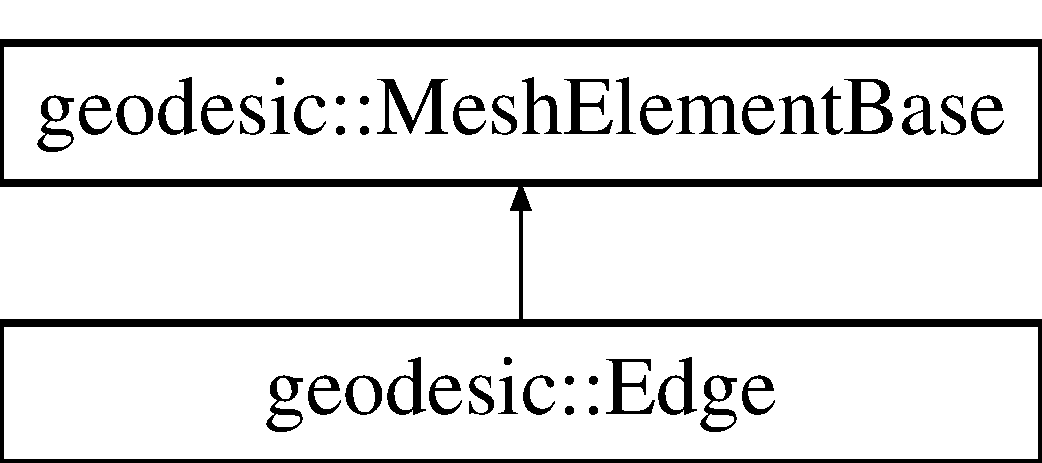
\includegraphics[height=2.000000cm]{classgeodesic_1_1_edge}
\end{center}
\end{figure}
\subsection*{Public Member Functions}
\begin{DoxyCompactItemize}
\item 
\hypertarget{classgeodesic_1_1_edge_a86095909b50a3a0feb2a0b9e8ac18ff8}{}double \& {\bfseries length} ()\label{classgeodesic_1_1_edge_a86095909b50a3a0feb2a0b9e8ac18ff8}

\item 
\hypertarget{classgeodesic_1_1_edge_ac6e6b51974a7b3c7a6a7cd48134c683c}{}\hyperlink{classgeodesic_1_1_face}{face\+\_\+pointer} {\bfseries opposite\+\_\+face} (\hyperlink{classgeodesic_1_1_face}{face\+\_\+pointer} f)\label{classgeodesic_1_1_edge_ac6e6b51974a7b3c7a6a7cd48134c683c}

\item 
\hypertarget{classgeodesic_1_1_edge_a353dcdc7f799bec55ef86e9248d55d01}{}\hyperlink{classgeodesic_1_1_vertex}{vertex\+\_\+pointer} {\bfseries opposite\+\_\+vertex} (\hyperlink{classgeodesic_1_1_vertex}{vertex\+\_\+pointer} v)\label{classgeodesic_1_1_edge_a353dcdc7f799bec55ef86e9248d55d01}

\item 
\hypertarget{classgeodesic_1_1_edge_a06ac8fdd1eb01bfccfb80dccf22e7600}{}bool {\bfseries belongs} (\hyperlink{classgeodesic_1_1_vertex}{vertex\+\_\+pointer} v)\label{classgeodesic_1_1_edge_a06ac8fdd1eb01bfccfb80dccf22e7600}

\item 
\hypertarget{classgeodesic_1_1_edge_a905bdb2e23940ed68c433e34afd44d31}{}bool {\bfseries is\+\_\+boundary} ()\label{classgeodesic_1_1_edge_a905bdb2e23940ed68c433e34afd44d31}

\item 
\hypertarget{classgeodesic_1_1_edge_aae82810e465b89e54df4643446b38059}{}\hyperlink{classgeodesic_1_1_vertex}{vertex\+\_\+pointer} {\bfseries v0} ()\label{classgeodesic_1_1_edge_aae82810e465b89e54df4643446b38059}

\item 
\hypertarget{classgeodesic_1_1_edge_a3ec747bf09057f61abea8da527a9e86e}{}\hyperlink{classgeodesic_1_1_vertex}{vertex\+\_\+pointer} {\bfseries v1} ()\label{classgeodesic_1_1_edge_a3ec747bf09057f61abea8da527a9e86e}

\item 
\hypertarget{classgeodesic_1_1_edge_a8c4e0d1f248b1e0a669b6666fa8398e0}{}void {\bfseries local\+\_\+coordinates} (\hyperlink{classgeodesic_1_1_point3_d}{Point3\+D} $\ast$point, double \&x, double \&y)\label{classgeodesic_1_1_edge_a8c4e0d1f248b1e0a669b6666fa8398e0}

\end{DoxyCompactItemize}
\subsection*{Additional Inherited Members}


The documentation for this class was generated from the following file\+:\begin{DoxyCompactItemize}
\item 
src/domain/metric/3rdparty/geodesic/geodesic\+\_\+mesh\+\_\+elements.\+h\end{DoxyCompactItemize}

\hypertarget{structgeodesic_1_1edge__visible__from__source}{}\section{geodesic\+:\+:edge\+\_\+visible\+\_\+from\+\_\+source Struct Reference}
\label{structgeodesic_1_1edge__visible__from__source}\index{geodesic\+::edge\+\_\+visible\+\_\+from\+\_\+source@{geodesic\+::edge\+\_\+visible\+\_\+from\+\_\+source}}
\subsection*{Public Attributes}
\begin{DoxyCompactItemize}
\item 
\hypertarget{structgeodesic_1_1edge__visible__from__source_a288acfdd8aba7d6eaebde69d1c19ee9b}{}unsigned {\bfseries source}\label{structgeodesic_1_1edge__visible__from__source_a288acfdd8aba7d6eaebde69d1c19ee9b}

\item 
\hypertarget{structgeodesic_1_1edge__visible__from__source_a5509a26ed330e5ba07748c8d3f8ef8a7}{}\hyperlink{classgeodesic_1_1_edge}{edge\+\_\+pointer} {\bfseries edge}\label{structgeodesic_1_1edge__visible__from__source_a5509a26ed330e5ba07748c8d3f8ef8a7}

\end{DoxyCompactItemize}


The documentation for this struct was generated from the following file\+:\begin{DoxyCompactItemize}
\item 
src/domain/metric/3rdparty/geodesic/geodesic\+\_\+mesh.\+h\end{DoxyCompactItemize}

\hypertarget{class_error_observer}{}\section{Error\+Observer Class Reference}
\label{class_error_observer}\index{Error\+Observer@{Error\+Observer}}
Inheritance diagram for Error\+Observer\+:\begin{figure}[H]
\begin{center}
\leavevmode
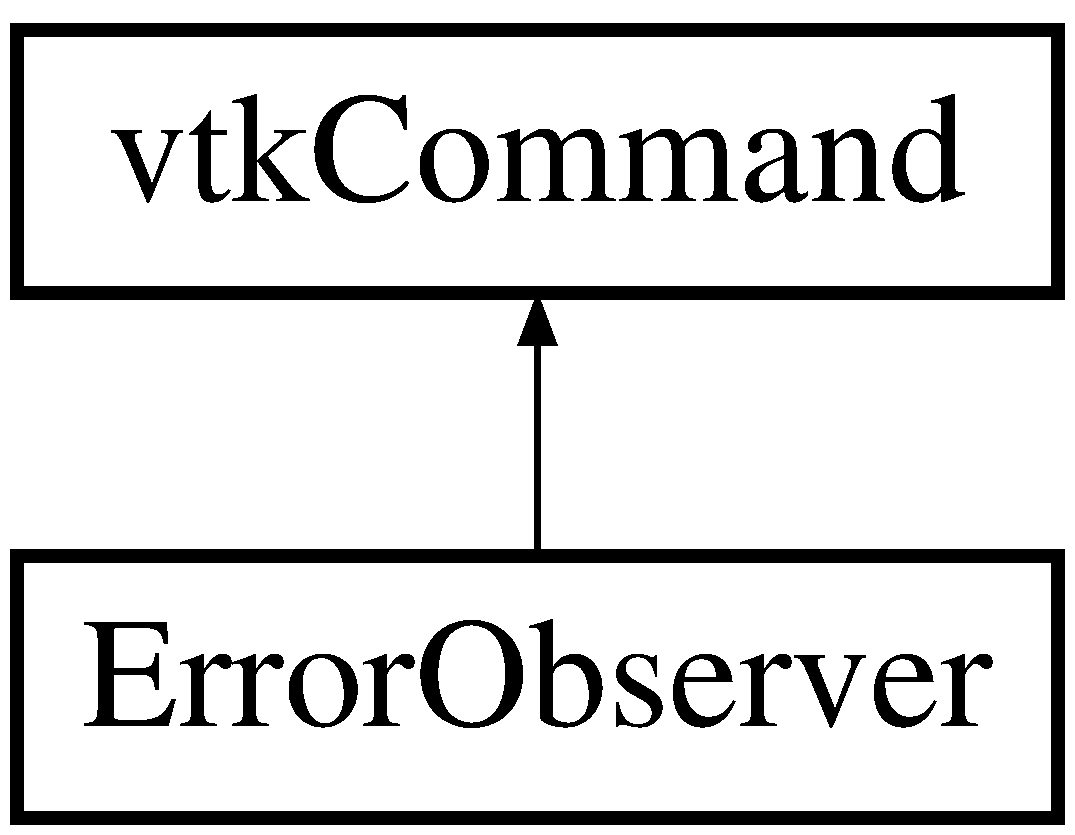
\includegraphics[height=2.000000cm]{class_error_observer}
\end{center}
\end{figure}
\subsection*{Public Member Functions}
\begin{DoxyCompactItemize}
\item 
\hypertarget{class_error_observer_a9e8da079cec071e384ddaa6e97af84c9}{}bool {\bfseries Get\+Error} () const \label{class_error_observer_a9e8da079cec071e384ddaa6e97af84c9}

\item 
\hypertarget{class_error_observer_a91d1cf38346f8973d3cd915d8f8946ae}{}bool {\bfseries Get\+Warning} () const \label{class_error_observer_a91d1cf38346f8973d3cd915d8f8946ae}

\item 
\hypertarget{class_error_observer_a368511a8ecda76d9681739ddc5588a5d}{}void {\bfseries Clear} ()\label{class_error_observer_a368511a8ecda76d9681739ddc5588a5d}

\item 
\hypertarget{class_error_observer_af2bebb0e4aa18f6b1c260ef7aa9ee55d}{}virtual void {\bfseries Execute} (vtk\+Object $\ast$vtk\+Not\+Used(caller), unsigned long event, void $\ast$calldata)\label{class_error_observer_af2bebb0e4aa18f6b1c260ef7aa9ee55d}

\item 
\hypertarget{class_error_observer_a97218477be7fa8ea2643d4ee8c691b03}{}std\+::string {\bfseries Get\+Error\+Message} ()\label{class_error_observer_a97218477be7fa8ea2643d4ee8c691b03}

\item 
\hypertarget{class_error_observer_ab5f5b9a966760a173fb123e14c02a081}{}std\+::string {\bfseries Get\+Warning\+Message} ()\label{class_error_observer_ab5f5b9a966760a173fb123e14c02a081}

\end{DoxyCompactItemize}
\subsection*{Static Public Member Functions}
\begin{DoxyCompactItemize}
\item 
\hypertarget{class_error_observer_a6ff871db01ac3aaf8152e715faf8dd9d}{}static \hyperlink{class_error_observer}{Error\+Observer} $\ast$ {\bfseries New} ()\label{class_error_observer_a6ff871db01ac3aaf8152e715faf8dd9d}

\end{DoxyCompactItemize}


The documentation for this class was generated from the following file\+:\begin{DoxyCompactItemize}
\item 
src/view/Error\+Observer.\+h\end{DoxyCompactItemize}

\hypertarget{class_euclidean_metric}{}\section{Euclidean\+Metric Class Reference}
\label{class_euclidean_metric}\index{Euclidean\+Metric@{Euclidean\+Metric}}
Inheritance diagram for Euclidean\+Metric\+:\begin{figure}[H]
\begin{center}
\leavevmode
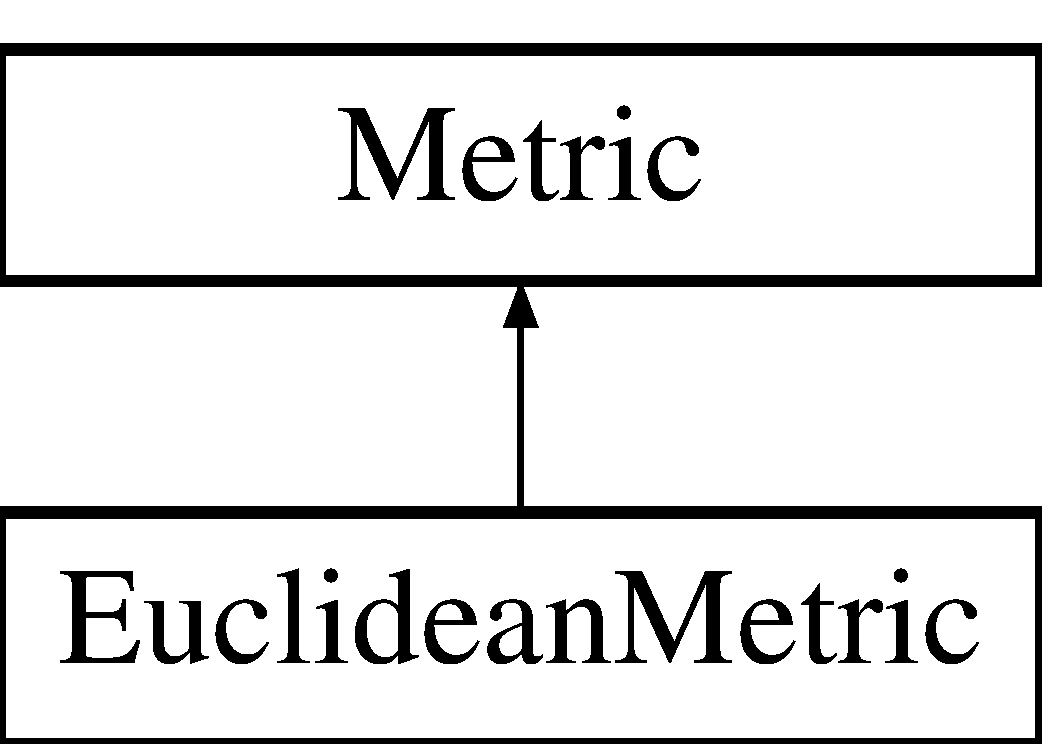
\includegraphics[height=2.000000cm]{class_euclidean_metric}
\end{center}
\end{figure}
\subsection*{Public Member Functions}
\begin{DoxyCompactItemize}
\item 
\hypertarget{class_euclidean_metric_a315e2486b0aaea14c64872d345dc235c}{}virtual double {\bfseries get\+Distance} (vtk\+Id\+Type a, vtk\+Id\+Type b)\label{class_euclidean_metric_a315e2486b0aaea14c64872d345dc235c}

\item 
\hypertarget{class_euclidean_metric_a16d8796d187eb9befe46fb5ed45a710f}{}virtual void {\bfseries get\+All\+Distances} (\hyperlink{class_scalar_point_attribute}{Scalar\+Point\+Attribute} \&distances, vtk\+Id\+Type source)\label{class_euclidean_metric_a16d8796d187eb9befe46fb5ed45a710f}

\item 
\hypertarget{class_euclidean_metric_a03f0ee77bcb02777044a4a86da79e9f5}{}virtual vtk\+Smart\+Pointer$<$ vtk\+Id\+List $>$ {\bfseries get\+Voronoi\+Cells} (vtk\+Smart\+Pointer$<$ vtk\+Id\+List $>$ seeds)\label{class_euclidean_metric_a03f0ee77bcb02777044a4a86da79e9f5}

\item 
\hypertarget{class_euclidean_metric_abbbcff587376543750466b297968c48c}{}virtual vtk\+Id\+Type {\bfseries get\+Farthest\+Point} (vtk\+Smart\+Pointer$<$ vtk\+Id\+List $>$ sources)\label{class_euclidean_metric_abbbcff587376543750466b297968c48c}

\end{DoxyCompactItemize}
\subsection*{Static Public Member Functions}
\begin{DoxyCompactItemize}
\item 
\hypertarget{class_euclidean_metric_a071547839c764daa6ccbfea7e5b90f67}{}static \hyperlink{class_metric}{Metric} $\ast$ {\bfseries create} ()\label{class_euclidean_metric_a071547839c764daa6ccbfea7e5b90f67}

\item 
\hypertarget{class_euclidean_metric_aae3729a99847724320e0f969d5af85e7}{}static string {\bfseries get\+Identifier} ()\label{class_euclidean_metric_aae3729a99847724320e0f969d5af85e7}

\end{DoxyCompactItemize}
\subsection*{Additional Inherited Members}


The documentation for this class was generated from the following files\+:\begin{DoxyCompactItemize}
\item 
src/domain/metric/Euclidean\+Metric.\+h\item 
src/domain/metric/Euclidean\+Metric.\+cpp\end{DoxyCompactItemize}

\hypertarget{classgeodesic_1_1_face}{}\section{geodesic\+:\+:Face Class Reference}
\label{classgeodesic_1_1_face}\index{geodesic\+::\+Face@{geodesic\+::\+Face}}
Inheritance diagram for geodesic\+:\+:Face\+:\begin{figure}[H]
\begin{center}
\leavevmode
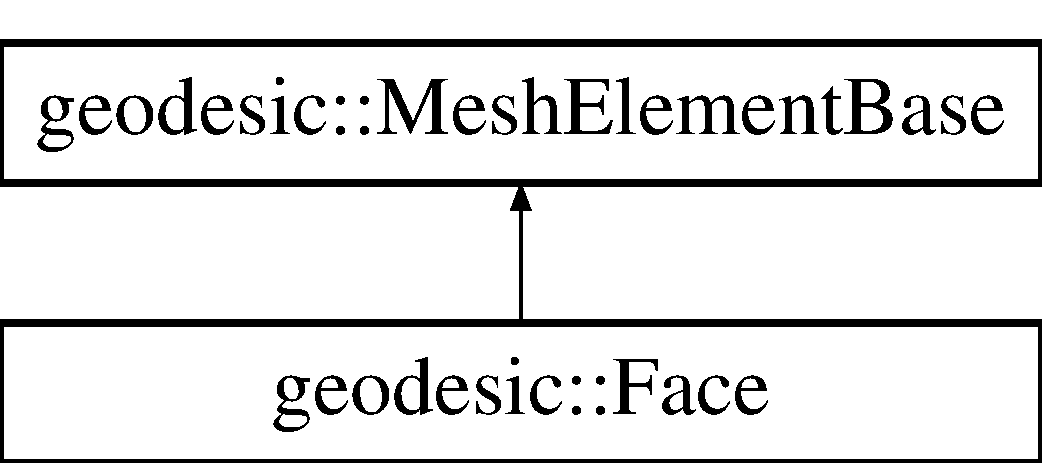
\includegraphics[height=2.000000cm]{classgeodesic_1_1_face}
\end{center}
\end{figure}
\subsection*{Public Member Functions}
\begin{DoxyCompactItemize}
\item 
\hypertarget{classgeodesic_1_1_face_a53b7a1245ad6ae15b074795e842b29f8}{}\hyperlink{classgeodesic_1_1_edge}{edge\+\_\+pointer} {\bfseries opposite\+\_\+edge} (\hyperlink{classgeodesic_1_1_vertex}{vertex\+\_\+pointer} v)\label{classgeodesic_1_1_face_a53b7a1245ad6ae15b074795e842b29f8}

\item 
\hypertarget{classgeodesic_1_1_face_a1019346a7b365a584bba05df2e8007b8}{}\hyperlink{classgeodesic_1_1_vertex}{vertex\+\_\+pointer} {\bfseries opposite\+\_\+vertex} (\hyperlink{classgeodesic_1_1_edge}{edge\+\_\+pointer} e)\label{classgeodesic_1_1_face_a1019346a7b365a584bba05df2e8007b8}

\item 
\hypertarget{classgeodesic_1_1_face_a55006ee598a9a1a379607b45f3195e89}{}\hyperlink{classgeodesic_1_1_edge}{edge\+\_\+pointer} {\bfseries next\+\_\+edge} (\hyperlink{classgeodesic_1_1_edge}{edge\+\_\+pointer} e, \hyperlink{classgeodesic_1_1_vertex}{vertex\+\_\+pointer} v)\label{classgeodesic_1_1_face_a55006ee598a9a1a379607b45f3195e89}

\item 
\hypertarget{classgeodesic_1_1_face_ad4aaaff39977cc3ef9774d65b2833821}{}double {\bfseries vertex\+\_\+angle} (\hyperlink{classgeodesic_1_1_vertex}{vertex\+\_\+pointer} v)\label{classgeodesic_1_1_face_ad4aaaff39977cc3ef9774d65b2833821}

\item 
\hypertarget{classgeodesic_1_1_face_a3c73256fa53edb4f8f285db219dc97bd}{}double $\ast$ {\bfseries corner\+\_\+angles} ()\label{classgeodesic_1_1_face_a3c73256fa53edb4f8f285db219dc97bd}

\end{DoxyCompactItemize}
\subsection*{Additional Inherited Members}


The documentation for this class was generated from the following file\+:\begin{DoxyCompactItemize}
\item 
src/domain/metric/3rdparty/geodesic/geodesic\+\_\+mesh\+\_\+elements.\+h\end{DoxyCompactItemize}

\hypertarget{class_face_coordinate_coloring}{}\section{Face\+Coordinate\+Coloring Class Reference}
\label{class_face_coordinate_coloring}\index{Face\+Coordinate\+Coloring@{Face\+Coordinate\+Coloring}}
Inheritance diagram for Face\+Coordinate\+Coloring\+:\begin{figure}[H]
\begin{center}
\leavevmode
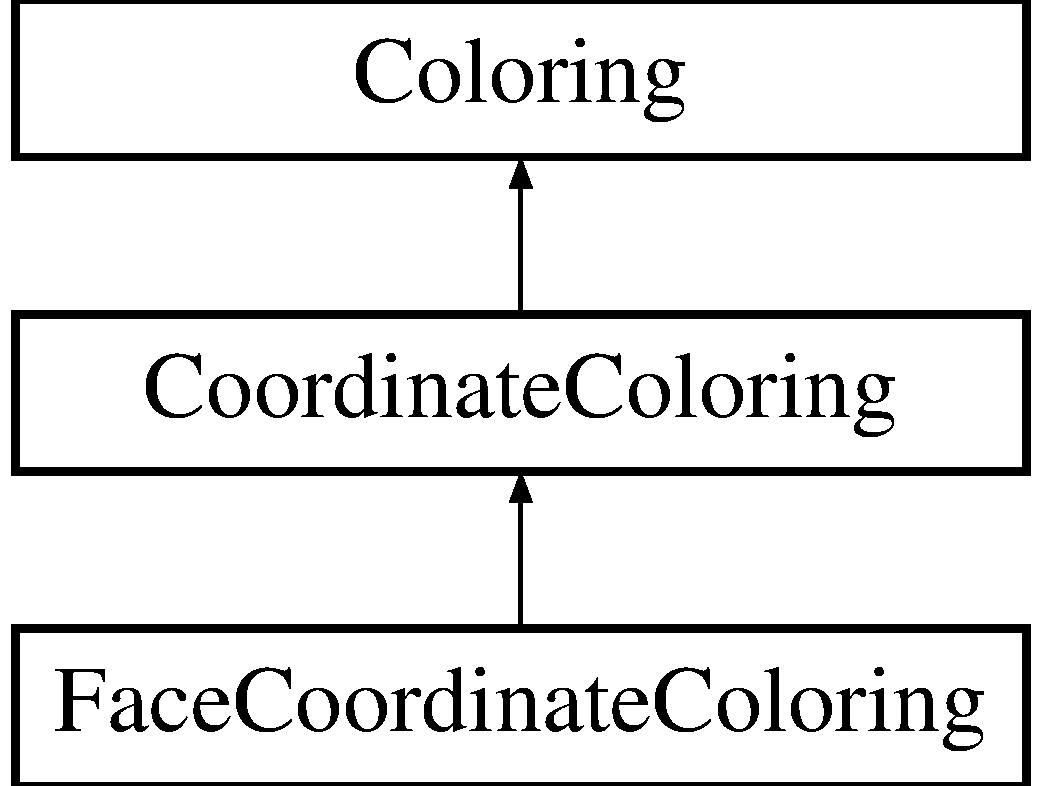
\includegraphics[height=3.000000cm]{class_face_coordinate_coloring}
\end{center}
\end{figure}
\subsection*{Public Member Functions}
\begin{DoxyCompactItemize}
\item 
\hypertarget{class_face_coordinate_coloring_a4fc5101b5447c9ac5f4ea293ed389d11}{}{\bfseries Face\+Coordinate\+Coloring} (\hyperlink{class_shape}{Shape} $\ast$shape)\label{class_face_coordinate_coloring_a4fc5101b5447c9ac5f4ea293ed389d11}

\item 
\hypertarget{class_face_coordinate_coloring_a23935c52a6d31a017e8fb3e17c144cb5}{}virtual void {\bfseries color} ()\label{class_face_coordinate_coloring_a23935c52a6d31a017e8fb3e17c144cb5}

\item 
\hypertarget{class_face_coordinate_coloring_a45397f5e7e5910df62be4c8d7cfeaf8a}{}vtk\+Smart\+Pointer$<$ vtk\+Unsigned\+Char\+Array $>$ {\bfseries get\+Colors} ()\label{class_face_coordinate_coloring_a45397f5e7e5910df62be4c8d7cfeaf8a}

\end{DoxyCompactItemize}
\subsection*{Additional Inherited Members}


The documentation for this class was generated from the following file\+:\begin{DoxyCompactItemize}
\item 
src/domain/coloring/Face\+Coordinate\+Coloring.\+h\end{DoxyCompactItemize}

\hypertarget{class_face_correspondence}{}\section{Face\+Correspondence Class Reference}
\label{class_face_correspondence}\index{Face\+Correspondence@{Face\+Correspondence}}
Inheritance diagram for Face\+Correspondence\+:\begin{figure}[H]
\begin{center}
\leavevmode
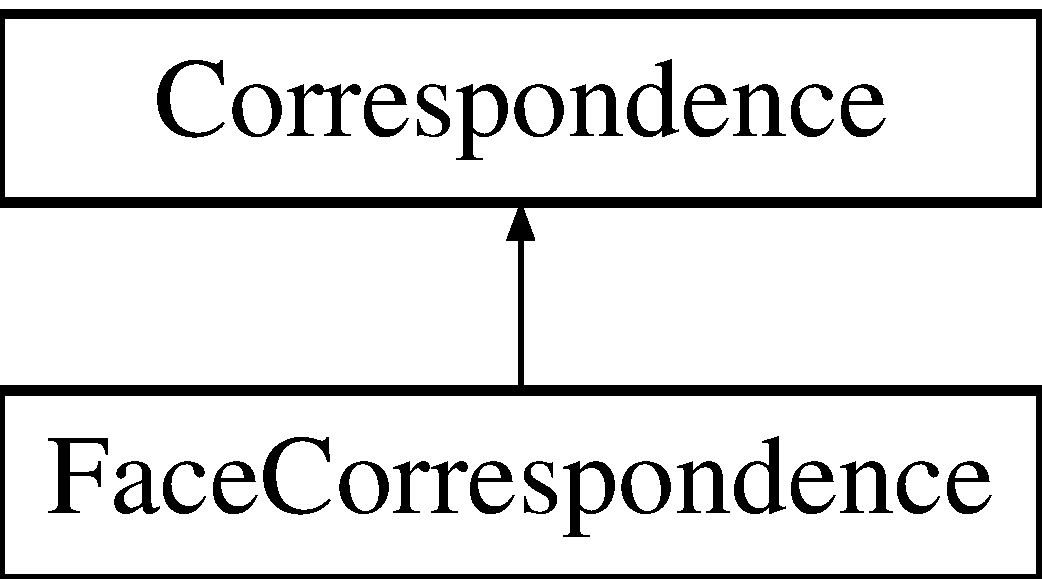
\includegraphics[height=2.000000cm]{class_face_correspondence}
\end{center}
\end{figure}
\subsection*{Public Member Functions}
\begin{DoxyCompactItemize}
\item 
\hypertarget{class_face_correspondence_a1bc50409e9b90564cf20ca94fcf1f177}{}{\bfseries Face\+Correspondence} (vtk\+Smart\+Pointer$<$ vtk\+Renderer $>$ renderer, \hyperlink{class_face_correspondence_data}{Face\+Correspondence\+Data} $\ast$data)\label{class_face_correspondence_a1bc50409e9b90564cf20ca94fcf1f177}

\item 
\hypertarget{class_face_correspondence_a08368a1caf1f848f25e8cb20b5dda5b4}{}{\bfseries Face\+Correspondence} (vtk\+Smart\+Pointer$<$ vtk\+Renderer $>$ renderer, \hyperlink{class_face_correspondence_data}{Face\+Correspondence\+Data} $\ast$data, \hyperlink{class_hash_map}{Hash\+Map}$<$ vtk\+Actor $\ast$, \hyperlink{class_shape}{Shape} $\ast$ $>$ \&shapes)\label{class_face_correspondence_a08368a1caf1f848f25e8cb20b5dda5b4}

\item 
\hypertarget{class_face_correspondence_afc6dbc51848ce528a0881f5f67a6116a}{}\hyperlink{class_face_correspondence_data}{Face\+Correspondence\+Data} $\ast$ {\bfseries get\+Data} ()\label{class_face_correspondence_afc6dbc51848ce528a0881f5f67a6116a}

\end{DoxyCompactItemize}
\subsection*{Protected Member Functions}
\begin{DoxyCompactItemize}
\item 
\hypertarget{class_face_correspondence_a1ea27f04de756e160ed0d80d2a685906}{}virtual void {\bfseries initialize\+Actor} (vtk\+Smart\+Pointer$<$ vtk\+Actor $>$ actor, \hyperlink{class_shape}{Shape} $\ast$shape, vtk\+Id\+Type face\+Id)\label{class_face_correspondence_a1ea27f04de756e160ed0d80d2a685906}

\item 
\hypertarget{class_face_correspondence_ac0314fcce59a91ed60a1a5cf9e7eec82}{}virtual void {\bfseries get\+Correspondence\+Point} (double point\mbox{[}3\mbox{]}, \hyperlink{class_shape}{Shape} $\ast$shape, vtk\+Id\+Type)\label{class_face_correspondence_ac0314fcce59a91ed60a1a5cf9e7eec82}

\end{DoxyCompactItemize}
\subsection*{Additional Inherited Members}


The documentation for this class was generated from the following files\+:\begin{DoxyCompactItemize}
\item 
src/domain/correspondences/Face\+Correspondence.\+h\item 
src/domain/correspondences/Face\+Correspondence.\+cpp\end{DoxyCompactItemize}

\hypertarget{class_face_correspondence_data}{}\section{Face\+Correspondence\+Data Class Reference}
\label{class_face_correspondence_data}\index{Face\+Correspondence\+Data@{Face\+Correspondence\+Data}}
Inheritance diagram for Face\+Correspondence\+Data\+:\begin{figure}[H]
\begin{center}
\leavevmode
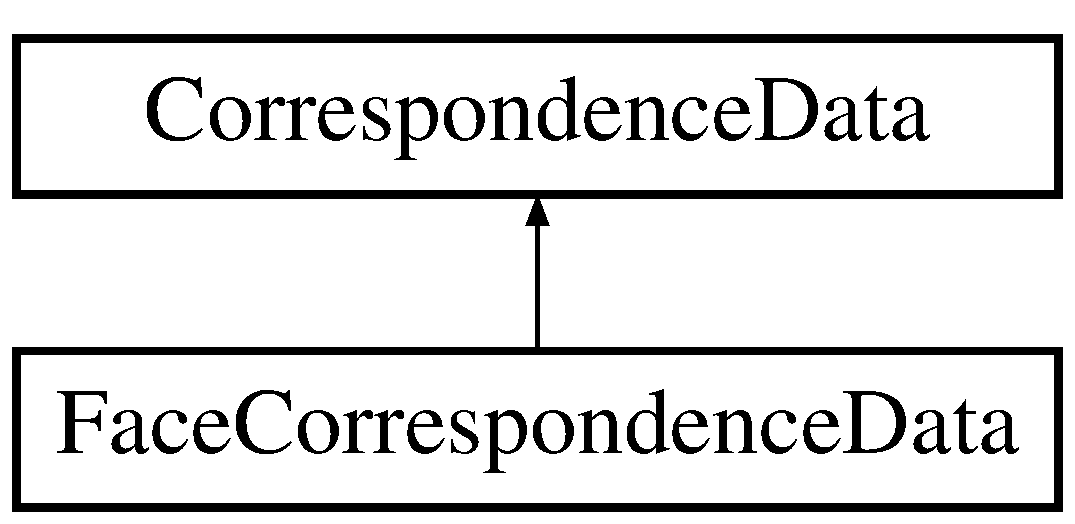
\includegraphics[height=2.000000cm]{class_face_correspondence_data}
\end{center}
\end{figure}
\subsection*{Public Member Functions}
\begin{DoxyCompactItemize}
\item 
\hypertarget{class_face_correspondence_data_a4890aed4edbf7842c051b121c30135bd}{}{\bfseries Face\+Correspondence\+Data} (vtk\+Id\+Type id)\label{class_face_correspondence_data_a4890aed4edbf7842c051b121c30135bd}

\item 
\hypertarget{class_face_correspondence_data_abd6ce7468457b56e5e093915591a1b17}{}virtual string {\bfseries get\+Type} ()\label{class_face_correspondence_data_abd6ce7468457b56e5e093915591a1b17}

\end{DoxyCompactItemize}
\subsection*{Additional Inherited Members}


The documentation for this class was generated from the following file\+:\begin{DoxyCompactItemize}
\item 
src/domain/correspondences/Face\+Correspondence\+Data.\+h\end{DoxyCompactItemize}

\hypertarget{class_face_correspondence_picker}{}\section{Face\+Correspondence\+Picker Class Reference}
\label{class_face_correspondence_picker}\index{Face\+Correspondence\+Picker@{Face\+Correspondence\+Picker}}
Inheritance diagram for Face\+Correspondence\+Picker\+:\begin{figure}[H]
\begin{center}
\leavevmode
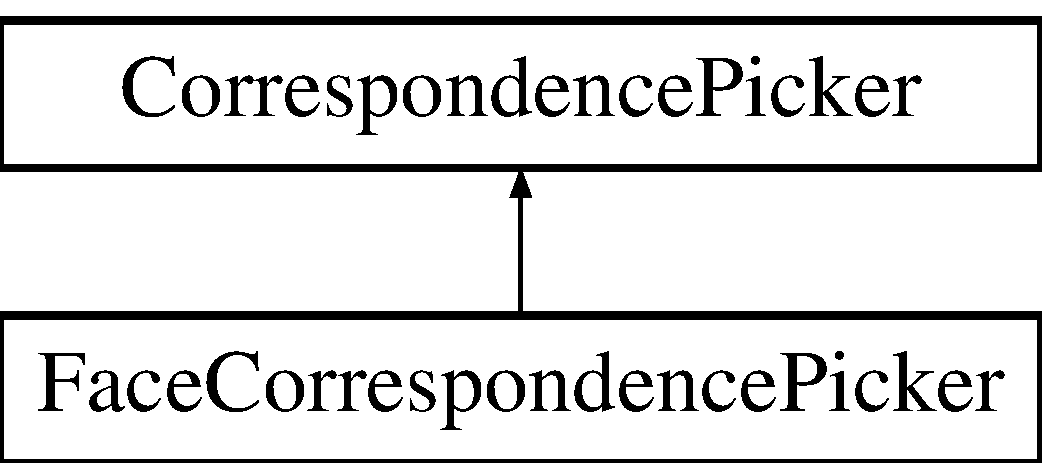
\includegraphics[height=2.000000cm]{class_face_correspondence_picker}
\end{center}
\end{figure}
\subsection*{Public Member Functions}
\begin{DoxyCompactItemize}
\item 
\hypertarget{class_face_correspondence_picker_afe96b5ac734a37e06f3be9723e552835}{}{\bfseries Face\+Correspondence\+Picker} (vtk\+Renderer $\ast$renderer, int \&last\+Insert\+Correspondence\+I\+D)\label{class_face_correspondence_picker_afe96b5ac734a37e06f3be9723e552835}

\end{DoxyCompactItemize}
\subsection*{Additional Inherited Members}


The documentation for this class was generated from the following files\+:\begin{DoxyCompactItemize}
\item 
src/view/Face\+Correspondence\+Picker.\+h\item 
src/view/Face\+Correspondence\+Picker.\+cpp\end{DoxyCompactItemize}

\hypertarget{class_ui_1_1_face_correspondences_widget}{}\section{Ui\+:\+:Face\+Correspondences\+Widget Class Reference}
\label{class_ui_1_1_face_correspondences_widget}\index{Ui\+::\+Face\+Correspondences\+Widget@{Ui\+::\+Face\+Correspondences\+Widget}}
Inheritance diagram for Ui\+:\+:Face\+Correspondences\+Widget\+:\begin{figure}[H]
\begin{center}
\leavevmode
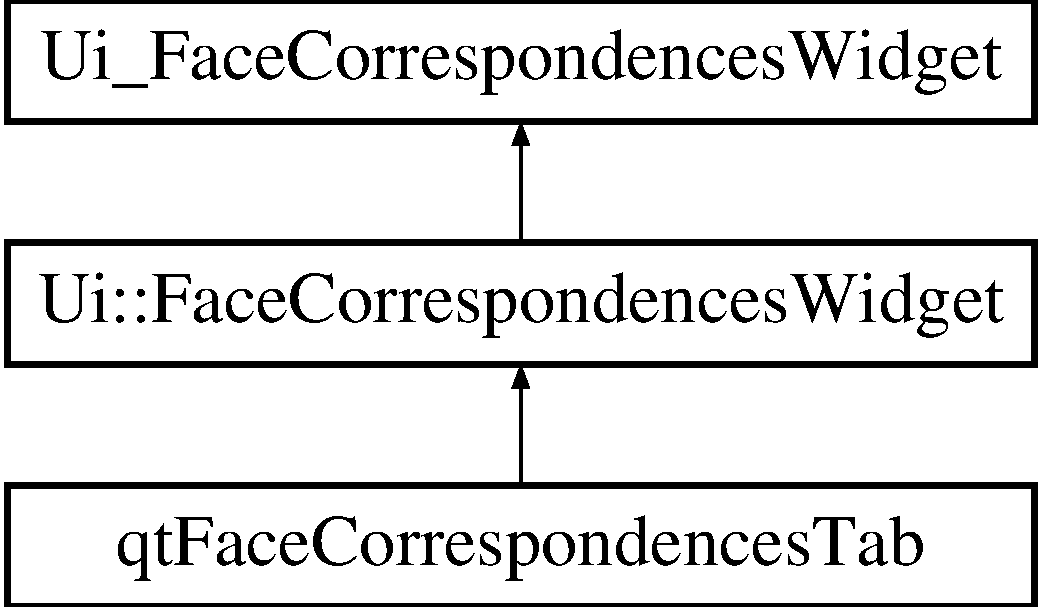
\includegraphics[height=3.000000cm]{class_ui_1_1_face_correspondences_widget}
\end{center}
\end{figure}
\subsection*{Additional Inherited Members}


The documentation for this class was generated from the following file\+:\begin{DoxyCompactItemize}
\item 
build/ui\+\_\+face\+Correspondences.\+h\end{DoxyCompactItemize}

\hypertarget{class_factory}{}\section{Factory$<$ T $>$ Class Template Reference}
\label{class_factory}\index{Factory$<$ T $>$@{Factory$<$ T $>$}}
\subsection*{Public Types}
\begin{DoxyCompactItemize}
\item 
\hypertarget{class_factory_ac84d352680c5cda7b6b15025f4fa0b8b}{}typedef T $\ast$($\ast$ {\bfseries Create\+Fn}) (void)\label{class_factory_ac84d352680c5cda7b6b15025f4fa0b8b}

\end{DoxyCompactItemize}
\subsection*{Public Member Functions}
\begin{DoxyCompactItemize}
\item 
\hypertarget{class_factory_a032a0ba3eeb8e43201c2a34ebacfbd57}{}{\footnotesize template$<$class C $>$ }\\void {\bfseries Register} (const string \&label)\label{class_factory_a032a0ba3eeb8e43201c2a34ebacfbd57}

\item 
\hypertarget{class_factory_a7fad946e94c6f33cf1f801d4bcdb3ce8}{}T $\ast$ {\bfseries create} (const string \&identifier)\label{class_factory_a7fad946e94c6f33cf1f801d4bcdb3ce8}

\item 
\hypertarget{class_factory_aa3b6b6cf2034462ad4a08564173f2574}{}{\footnotesize template$<$class C $>$ }\\T $\ast$ {\bfseries create} ()\label{class_factory_aa3b6b6cf2034462ad4a08564173f2574}

\item 
\hypertarget{class_factory_a0ec1bcb787080ddf713f19b61b47e6a0}{}unordered\+\_\+map$<$ string, string $>$ \& {\bfseries get\+Labels} ()\label{class_factory_a0ec1bcb787080ddf713f19b61b47e6a0}

\end{DoxyCompactItemize}
\subsection*{Static Public Member Functions}
\begin{DoxyCompactItemize}
\item 
\hypertarget{class_factory_a8a05f8e1a60d57e297509a7a483cb46a}{}static \hyperlink{class_factory}{Factory}$<$ T $>$ $\ast$ {\bfseries get\+Instance} ()\label{class_factory_a8a05f8e1a60d57e297509a7a483cb46a}

\end{DoxyCompactItemize}


The documentation for this class was generated from the following file\+:\begin{DoxyCompactItemize}
\item 
src/domain/Factory.\+h\end{DoxyCompactItemize}

\hypertarget{class_farthest_point_sampling}{}\section{Farthest\+Point\+Sampling Class Reference}
\label{class_farthest_point_sampling}\index{Farthest\+Point\+Sampling@{Farthest\+Point\+Sampling}}
Inheritance diagram for Farthest\+Point\+Sampling\+:\begin{figure}[H]
\begin{center}
\leavevmode
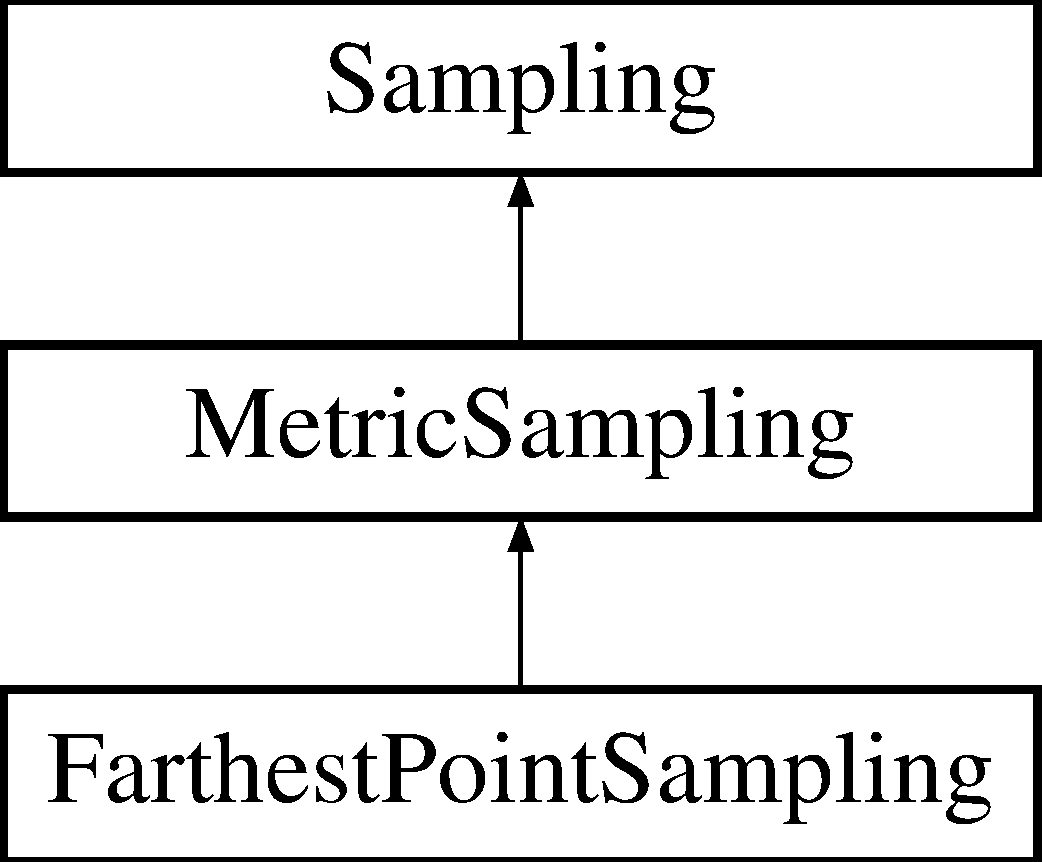
\includegraphics[height=3.000000cm]{class_farthest_point_sampling}
\end{center}
\end{figure}
\subsection*{Public Member Functions}
\begin{DoxyCompactItemize}
\item 
\hypertarget{class_farthest_point_sampling_a11fb39b69f5405fe47864bf867e5578e}{}void {\bfseries set\+Source} (vtk\+Id\+Type source)\label{class_farthest_point_sampling_a11fb39b69f5405fe47864bf867e5578e}

\item 
\hypertarget{class_farthest_point_sampling_a4c7c351804be31817a96aafeb578d99b}{}virtual vtk\+Smart\+Pointer$<$ vtk\+Id\+List $>$ {\bfseries get\+Points} ()\label{class_farthest_point_sampling_a4c7c351804be31817a96aafeb578d99b}

\end{DoxyCompactItemize}
\subsection*{Static Public Member Functions}
\begin{DoxyCompactItemize}
\item 
\hypertarget{class_farthest_point_sampling_a72bb32dad66e35e712cfaaaeec381fe2}{}static \hyperlink{class_sampling}{Sampling} $\ast$ {\bfseries create} ()\label{class_farthest_point_sampling_a72bb32dad66e35e712cfaaaeec381fe2}

\item 
\hypertarget{class_farthest_point_sampling_ae80cd0e1c311eb9f60603bf2ae24a0d4}{}static string {\bfseries get\+Identifier} ()\label{class_farthest_point_sampling_ae80cd0e1c311eb9f60603bf2ae24a0d4}

\end{DoxyCompactItemize}
\subsection*{Additional Inherited Members}


The documentation for this class was generated from the following files\+:\begin{DoxyCompactItemize}
\item 
src/domain/samplings/Farthest\+Point\+Sampling.\+h\item 
src/domain/samplings/Farthest\+Point\+Sampling.\+cpp\end{DoxyCompactItemize}

\hypertarget{class_f_e_m_laplace_beltrami_operator}{}\section{F\+E\+M\+Laplace\+Beltrami\+Operator Class Reference}
\label{class_f_e_m_laplace_beltrami_operator}\index{F\+E\+M\+Laplace\+Beltrami\+Operator@{F\+E\+M\+Laplace\+Beltrami\+Operator}}
Inheritance diagram for F\+E\+M\+Laplace\+Beltrami\+Operator\+:\begin{figure}[H]
\begin{center}
\leavevmode
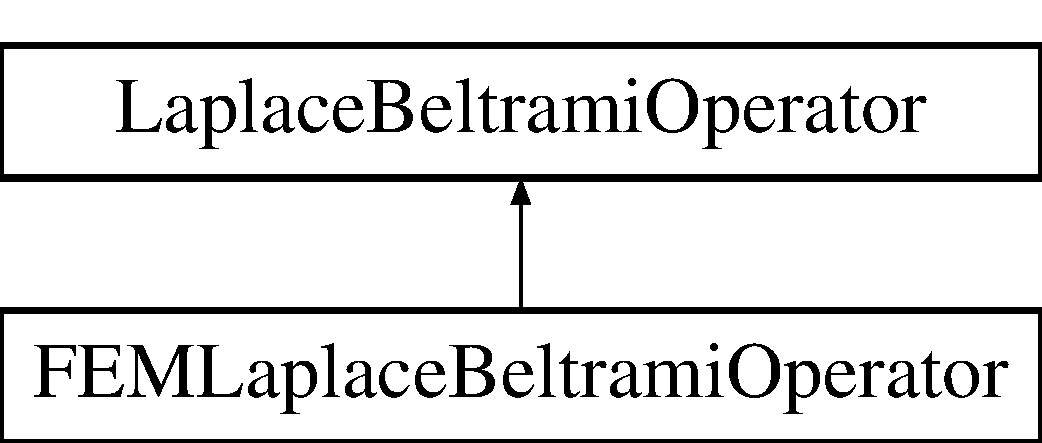
\includegraphics[height=2.000000cm]{class_f_e_m_laplace_beltrami_operator}
\end{center}
\end{figure}
\subsection*{Public Member Functions}
\begin{DoxyCompactItemize}
\item 
\hypertarget{class_f_e_m_laplace_beltrami_operator_a42bd51150afce240e48dbac75a6bc96b}{}virtual void {\bfseries initialize} (\hyperlink{class_shape}{Shape} $\ast$shape, int number\+Of\+Eigenfunctions)\label{class_f_e_m_laplace_beltrami_operator_a42bd51150afce240e48dbac75a6bc96b}

\item 
\hypertarget{class_f_e_m_laplace_beltrami_operator_a9e2d42cf84a9f24e2834621cd9b488df}{}virtual double {\bfseries get\+Eigenvalue} (int i)\label{class_f_e_m_laplace_beltrami_operator_a9e2d42cf84a9f24e2834621cd9b488df}

\item 
\hypertarget{class_f_e_m_laplace_beltrami_operator_af11d2968c30838048eaeea7fb2fc6395}{}virtual void {\bfseries get\+Eigenfunction} (int i, \hyperlink{class_scalar_point_attribute}{Scalar\+Point\+Attribute} \&phi)\label{class_f_e_m_laplace_beltrami_operator_af11d2968c30838048eaeea7fb2fc6395}

\item 
\hypertarget{class_f_e_m_laplace_beltrami_operator_a058af519fb64e4e7c6ea44c1383a864f}{}virtual void {\bfseries get\+Eigenfunction} (Petsc\+Int i, Vec $\ast$phi)\label{class_f_e_m_laplace_beltrami_operator_a058af519fb64e4e7c6ea44c1383a864f}

\item 
\hypertarget{class_f_e_m_laplace_beltrami_operator_a1b9cd4fca7b25131426d432030b53747}{}virtual void {\bfseries get\+Eigenpair} (Petsc\+Int i, Vec $\ast$phi, Petsc\+Scalar $\ast$lambda)\label{class_f_e_m_laplace_beltrami_operator_a1b9cd4fca7b25131426d432030b53747}

\item 
\hypertarget{class_f_e_m_laplace_beltrami_operator_a3d1bc2fb74325cb75bdcbcce57c24700}{}virtual Mat $\ast$ {\bfseries get\+Mass\+Matrix} ()\label{class_f_e_m_laplace_beltrami_operator_a3d1bc2fb74325cb75bdcbcce57c24700}

\item 
\hypertarget{class_f_e_m_laplace_beltrami_operator_a93a2063dfb32f86eb0973743631bccb1}{}Mat $\ast$ {\bfseries get\+Stiffness\+Matrix} ()\label{class_f_e_m_laplace_beltrami_operator_a93a2063dfb32f86eb0973743631bccb1}

\end{DoxyCompactItemize}
\subsection*{Static Public Member Functions}
\begin{DoxyCompactItemize}
\item 
\hypertarget{class_f_e_m_laplace_beltrami_operator_ab33dd874f3e8810a5ccac3d8a5d86a2a}{}static \hyperlink{class_laplace_beltrami_operator}{Laplace\+Beltrami\+Operator} $\ast$ {\bfseries create} ()\label{class_f_e_m_laplace_beltrami_operator_ab33dd874f3e8810a5ccac3d8a5d86a2a}

\item 
\hypertarget{class_f_e_m_laplace_beltrami_operator_a94bfc4fd93c40e4825626b8116bd5759}{}static string {\bfseries get\+Identifier} ()\label{class_f_e_m_laplace_beltrami_operator_a94bfc4fd93c40e4825626b8116bd5759}

\end{DoxyCompactItemize}
\subsection*{Additional Inherited Members}


The documentation for this class was generated from the following files\+:\begin{DoxyCompactItemize}
\item 
src/domain/F\+E\+M\+Laplace\+Beltrami\+Operator.\+h\item 
src/domain/F\+E\+M\+Laplace\+Beltrami\+Operator.\+cpp\end{DoxyCompactItemize}

\hypertarget{class_functional_maps}{}\section{Functional\+Maps Class Reference}
\label{class_functional_maps}\index{Functional\+Maps@{Functional\+Maps}}
\subsection*{Public Member Functions}
\begin{DoxyCompactItemize}
\item 
\hypertarget{class_functional_maps_ab1c62d698fff079b47e51d362ff30bbc}{}{\bfseries Functional\+Maps} (\hyperlink{class_shape}{Shape} \&shape1, \hyperlink{class_shape}{Shape} \&shape2, \hyperlink{class_laplace_beltrami_operator}{Laplace\+Beltrami\+Operator} $\ast$laplacian1, \hyperlink{class_laplace_beltrami_operator}{Laplace\+Beltrami\+Operator} $\ast$laplacian2, vector$<$ \hyperlink{class_scalar_point_attribute}{Scalar\+Point\+Attribute} $>$ \&c1, vector$<$ \hyperlink{class_scalar_point_attribute}{Scalar\+Point\+Attribute} $>$ \&c2, int number\+Of\+Eigenfunctions)\label{class_functional_maps_ab1c62d698fff079b47e51d362ff30bbc}

\item 
\hypertarget{class_functional_maps_ac5575986be9c4b00a497953e65084f4a}{}void {\bfseries transfer\+Function} (\hyperlink{class_scalar_point_attribute}{Scalar\+Point\+Attribute} \&f1, \hyperlink{class_scalar_point_attribute}{Scalar\+Point\+Attribute} \&f2)\label{class_functional_maps_ac5575986be9c4b00a497953e65084f4a}

\end{DoxyCompactItemize}


The documentation for this class was generated from the following files\+:\begin{DoxyCompactItemize}
\item 
src/domain/Functional\+Maps.\+h\item 
src/domain/Functional\+Maps.\+cpp\end{DoxyCompactItemize}

\hypertarget{classgeodesic__error}{}\section{geodesic\+\_\+error Class Reference}
\label{classgeodesic__error}\index{geodesic\+\_\+error@{geodesic\+\_\+error}}
\subsection*{Public Member Functions}
\begin{DoxyCompactItemize}
\item 
\hypertarget{classgeodesic__error_adcc7b4c1b2c96464cf807486fbc94c93}{}{\bfseries geodesic\+\_\+error} (std\+::string str)\label{classgeodesic__error_adcc7b4c1b2c96464cf807486fbc94c93}

\item 
\hypertarget{classgeodesic__error_ab51039328fe8a49a49cd71e4e0348507}{}std\+::string {\bfseries what} ()\label{classgeodesic__error_ab51039328fe8a49a49cd71e4e0348507}

\end{DoxyCompactItemize}


The documentation for this class was generated from the following file\+:\begin{DoxyCompactItemize}
\item 
src/domain/metric/3rdparty/geodesic/geodesic\+\_\+error.\+h\end{DoxyCompactItemize}

\hypertarget{classgeodesic_1_1_geodesic_algorithm_base}{}\section{geodesic\+:\+:Geodesic\+Algorithm\+Base Class Reference}
\label{classgeodesic_1_1_geodesic_algorithm_base}\index{geodesic\+::\+Geodesic\+Algorithm\+Base@{geodesic\+::\+Geodesic\+Algorithm\+Base}}
Inheritance diagram for geodesic\+:\+:Geodesic\+Algorithm\+Base\+:\begin{figure}[H]
\begin{center}
\leavevmode
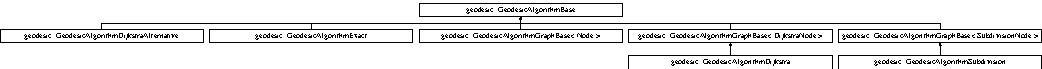
\includegraphics[height=0.920548cm]{classgeodesic_1_1_geodesic_algorithm_base}
\end{center}
\end{figure}
\subsection*{Public Types}
\begin{DoxyCompactItemize}
\item 
\hypertarget{classgeodesic_1_1_geodesic_algorithm_base_a92b104ecfd6664bba6e3e6089e62a568}{}enum {\bfseries Algorithm\+Type} \{ {\bfseries E\+X\+A\+C\+T}, 
{\bfseries D\+I\+J\+K\+S\+T\+R\+A}, 
{\bfseries S\+U\+B\+D\+I\+V\+I\+S\+I\+O\+N}, 
{\bfseries U\+N\+D\+E\+F\+I\+N\+E\+D\+\_\+\+A\+L\+G\+O\+R\+I\+T\+H\+M}
 \}\label{classgeodesic_1_1_geodesic_algorithm_base_a92b104ecfd6664bba6e3e6089e62a568}

\end{DoxyCompactItemize}
\subsection*{Public Member Functions}
\begin{DoxyCompactItemize}
\item 
\hypertarget{classgeodesic_1_1_geodesic_algorithm_base_a023f9fe21f67dbd0ed75be639f519c9c}{}{\bfseries Geodesic\+Algorithm\+Base} (\hyperlink{classgeodesic_1_1_mesh}{geodesic\+::\+Mesh} $\ast$mesh)\label{classgeodesic_1_1_geodesic_algorithm_base_a023f9fe21f67dbd0ed75be639f519c9c}

\item 
\hypertarget{classgeodesic_1_1_geodesic_algorithm_base_af1231184ca4215f90e5404dbfa05345e}{}virtual void {\bfseries propagate} (std\+::vector$<$ \hyperlink{classgeodesic_1_1_surface_point}{Surface\+Point} $>$ \&sources, double max\+\_\+propagation\+\_\+distance=G\+E\+O\+D\+E\+S\+I\+C\+\_\+\+I\+N\+F, std\+::vector$<$ \hyperlink{classgeodesic_1_1_surface_point}{Surface\+Point} $>$ $\ast$stop\+\_\+points=N\+U\+L\+L)=0\label{classgeodesic_1_1_geodesic_algorithm_base_af1231184ca4215f90e5404dbfa05345e}

\item 
\hypertarget{classgeodesic_1_1_geodesic_algorithm_base_a26d3226d68b102c74de5f8cca02472fe}{}virtual void {\bfseries trace\+\_\+back} (\hyperlink{classgeodesic_1_1_surface_point}{Surface\+Point} \&destination, std\+::vector$<$ \hyperlink{classgeodesic_1_1_surface_point}{Surface\+Point} $>$ \&path)=0\label{classgeodesic_1_1_geodesic_algorithm_base_a26d3226d68b102c74de5f8cca02472fe}

\item 
\hypertarget{classgeodesic_1_1_geodesic_algorithm_base_ad28b5eb5454e958c683647eb526543e4}{}void {\bfseries geodesic} (\hyperlink{classgeodesic_1_1_surface_point}{Surface\+Point} \&source, \hyperlink{classgeodesic_1_1_surface_point}{Surface\+Point} \&destination, std\+::vector$<$ \hyperlink{classgeodesic_1_1_surface_point}{Surface\+Point} $>$ \&path)\label{classgeodesic_1_1_geodesic_algorithm_base_ad28b5eb5454e958c683647eb526543e4}

\item 
\hypertarget{classgeodesic_1_1_geodesic_algorithm_base_afc459d5951c9be476c3997f225e09872}{}void {\bfseries geodesic} (std\+::vector$<$ \hyperlink{classgeodesic_1_1_surface_point}{Surface\+Point} $>$ \&sources, std\+::vector$<$ \hyperlink{classgeodesic_1_1_surface_point}{Surface\+Point} $>$ \&destinations, std\+::vector$<$ std\+::vector$<$ \hyperlink{classgeodesic_1_1_surface_point}{Surface\+Point} $>$ $>$ \&paths)\label{classgeodesic_1_1_geodesic_algorithm_base_afc459d5951c9be476c3997f225e09872}

\item 
\hypertarget{classgeodesic_1_1_geodesic_algorithm_base_a2cad02f242ef6781d451a539970a547a}{}virtual unsigned {\bfseries best\+\_\+source} (\hyperlink{classgeodesic_1_1_surface_point}{Surface\+Point} \&point, double \&best\+\_\+source\+\_\+distance)=0\label{classgeodesic_1_1_geodesic_algorithm_base_a2cad02f242ef6781d451a539970a547a}

\item 
\hypertarget{classgeodesic_1_1_geodesic_algorithm_base_a44790285937a918a466ed57cc22b327a}{}virtual void {\bfseries print\+\_\+statistics} ()\label{classgeodesic_1_1_geodesic_algorithm_base_a44790285937a918a466ed57cc22b327a}

\item 
\hypertarget{classgeodesic_1_1_geodesic_algorithm_base_a5618d753cb471af1b85c4d1843fd8bc9}{}Algorithm\+Type {\bfseries type} ()\label{classgeodesic_1_1_geodesic_algorithm_base_a5618d753cb471af1b85c4d1843fd8bc9}

\item 
\hypertarget{classgeodesic_1_1_geodesic_algorithm_base_abe7d6bf87ab38b9cbac85c84b17ebf4c}{}virtual std\+::string {\bfseries name} ()\label{classgeodesic_1_1_geodesic_algorithm_base_abe7d6bf87ab38b9cbac85c84b17ebf4c}

\item 
\hypertarget{classgeodesic_1_1_geodesic_algorithm_base_aeaeea45a3e01962834c160a1edbb68ef}{}\hyperlink{classgeodesic_1_1_mesh}{geodesic\+::\+Mesh} $\ast$ {\bfseries mesh} ()\label{classgeodesic_1_1_geodesic_algorithm_base_aeaeea45a3e01962834c160a1edbb68ef}

\end{DoxyCompactItemize}
\subsection*{Protected Types}
\begin{DoxyCompactItemize}
\item 
\hypertarget{classgeodesic_1_1_geodesic_algorithm_base_afc97d6ccbe2c1603793936ec38e6f3a8}{}typedef std\+::pair$<$ \hyperlink{classgeodesic_1_1_vertex}{vertex\+\_\+pointer}, double $>$ {\bfseries stop\+\_\+vertex\+\_\+with\+\_\+distace\+\_\+type}\label{classgeodesic_1_1_geodesic_algorithm_base_afc97d6ccbe2c1603793936ec38e6f3a8}

\end{DoxyCompactItemize}
\subsection*{Protected Member Functions}
\begin{DoxyCompactItemize}
\item 
\hypertarget{classgeodesic_1_1_geodesic_algorithm_base_a4f2040a2d68593a6c8792d46202bc5e6}{}void {\bfseries set\+\_\+stop\+\_\+conditions} (std\+::vector$<$ \hyperlink{classgeodesic_1_1_surface_point}{Surface\+Point} $>$ $\ast$stop\+\_\+points, double stop\+\_\+distance)\label{classgeodesic_1_1_geodesic_algorithm_base_a4f2040a2d68593a6c8792d46202bc5e6}

\item 
\hypertarget{classgeodesic_1_1_geodesic_algorithm_base_a0bb83e25e4ef90d92f6d79b783efd909}{}double {\bfseries stop\+\_\+distance} ()\label{classgeodesic_1_1_geodesic_algorithm_base_a0bb83e25e4ef90d92f6d79b783efd909}

\end{DoxyCompactItemize}
\subsection*{Protected Attributes}
\begin{DoxyCompactItemize}
\item 
\hypertarget{classgeodesic_1_1_geodesic_algorithm_base_acfae8cd7708554fc43c3a4de82706a68}{}Algorithm\+Type {\bfseries m\+\_\+type}\label{classgeodesic_1_1_geodesic_algorithm_base_acfae8cd7708554fc43c3a4de82706a68}

\item 
\hypertarget{classgeodesic_1_1_geodesic_algorithm_base_ad88f249e874b8445f3d92846bf39875f}{}std\+::vector$<$ stop\+\_\+vertex\+\_\+with\+\_\+distace\+\_\+type $>$ {\bfseries m\+\_\+stop\+\_\+vertices}\label{classgeodesic_1_1_geodesic_algorithm_base_ad88f249e874b8445f3d92846bf39875f}

\item 
\hypertarget{classgeodesic_1_1_geodesic_algorithm_base_ac4f8f7cc46da5fc1b013a3a9b83d0843}{}double {\bfseries m\+\_\+max\+\_\+propagation\+\_\+distance}\label{classgeodesic_1_1_geodesic_algorithm_base_ac4f8f7cc46da5fc1b013a3a9b83d0843}

\item 
\hypertarget{classgeodesic_1_1_geodesic_algorithm_base_a60c4d6e286af80a84875bf2a15ebf7dc}{}\hyperlink{classgeodesic_1_1_mesh}{geodesic\+::\+Mesh} $\ast$ {\bfseries m\+\_\+mesh}\label{classgeodesic_1_1_geodesic_algorithm_base_a60c4d6e286af80a84875bf2a15ebf7dc}

\item 
\hypertarget{classgeodesic_1_1_geodesic_algorithm_base_a5eab429056495d7709bb02d300d03e7a}{}double {\bfseries m\+\_\+time\+\_\+consumed}\label{classgeodesic_1_1_geodesic_algorithm_base_a5eab429056495d7709bb02d300d03e7a}

\item 
\hypertarget{classgeodesic_1_1_geodesic_algorithm_base_ac45e2667cee21ed383301029bfbcef9d}{}double {\bfseries m\+\_\+propagation\+\_\+distance\+\_\+stopped}\label{classgeodesic_1_1_geodesic_algorithm_base_ac45e2667cee21ed383301029bfbcef9d}

\end{DoxyCompactItemize}


The documentation for this class was generated from the following file\+:\begin{DoxyCompactItemize}
\item 
src/domain/metric/3rdparty/geodesic/geodesic\+\_\+algorithm\+\_\+base.\+h\end{DoxyCompactItemize}

\hypertarget{classgeodesic_1_1_geodesic_algorithm_dijkstra}{}\section{geodesic\+:\+:Geodesic\+Algorithm\+Dijkstra Class Reference}
\label{classgeodesic_1_1_geodesic_algorithm_dijkstra}\index{geodesic\+::\+Geodesic\+Algorithm\+Dijkstra@{geodesic\+::\+Geodesic\+Algorithm\+Dijkstra}}
Inheritance diagram for geodesic\+:\+:Geodesic\+Algorithm\+Dijkstra\+:\begin{figure}[H]
\begin{center}
\leavevmode
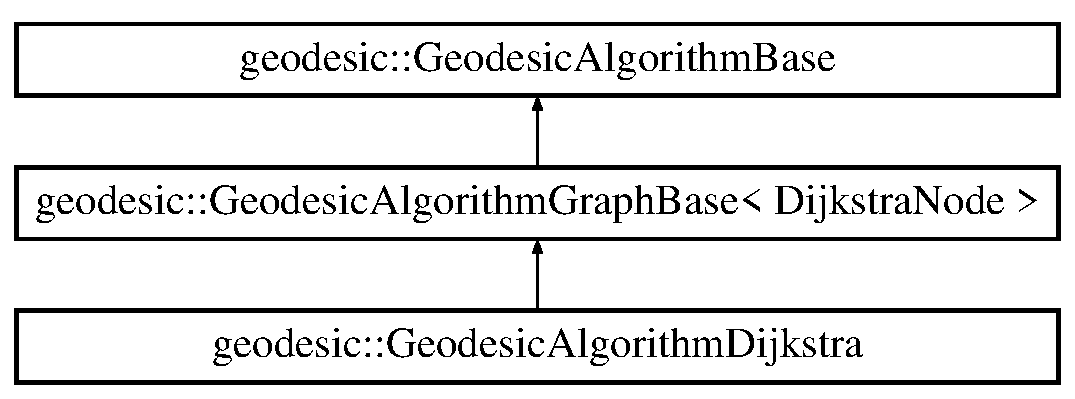
\includegraphics[height=3.000000cm]{classgeodesic_1_1_geodesic_algorithm_dijkstra}
\end{center}
\end{figure}
\subsection*{Public Types}
\begin{DoxyCompactItemize}
\item 
\hypertarget{classgeodesic_1_1_geodesic_algorithm_dijkstra_a457ff6fabaa767aea932160514c06b72}{}typedef \hyperlink{classgeodesic_1_1_dijkstra_node}{Dijkstra\+Node} {\bfseries Node}\label{classgeodesic_1_1_geodesic_algorithm_dijkstra_a457ff6fabaa767aea932160514c06b72}

\item 
\hypertarget{classgeodesic_1_1_geodesic_algorithm_dijkstra_ab534a34c7d8c4cd92743777c07a31dc5}{}typedef \hyperlink{classgeodesic_1_1_dijkstra_node}{Node} $\ast$ {\bfseries node\+\_\+pointer}\label{classgeodesic_1_1_geodesic_algorithm_dijkstra_ab534a34c7d8c4cd92743777c07a31dc5}

\end{DoxyCompactItemize}
\subsection*{Public Member Functions}
\begin{DoxyCompactItemize}
\item 
\hypertarget{classgeodesic_1_1_geodesic_algorithm_dijkstra_ae07f68dafa762828a23e31c6415947ae}{}{\bfseries Geodesic\+Algorithm\+Dijkstra} (\hyperlink{classgeodesic_1_1_mesh}{geodesic\+::\+Mesh} $\ast$mesh)\label{classgeodesic_1_1_geodesic_algorithm_dijkstra_ae07f68dafa762828a23e31c6415947ae}

\end{DoxyCompactItemize}
\subsection*{Protected Member Functions}
\begin{DoxyCompactItemize}
\item 
\hypertarget{classgeodesic_1_1_geodesic_algorithm_dijkstra_aeec97299e8830773b87c152b52ab42f1}{}void {\bfseries list\+\_\+nodes\+\_\+visible\+\_\+from\+\_\+source} (\hyperlink{classgeodesic_1_1_mesh_element_base}{Mesh\+Element\+Base} $\ast$p, std\+::vector$<$ \hyperlink{classgeodesic_1_1_dijkstra_node}{node\+\_\+pointer} $>$ \&storage)\label{classgeodesic_1_1_geodesic_algorithm_dijkstra_aeec97299e8830773b87c152b52ab42f1}

\item 
\hypertarget{classgeodesic_1_1_geodesic_algorithm_dijkstra_ad04ebd924efcc40d5c1dd8b31532a81a}{}void {\bfseries list\+\_\+nodes\+\_\+visible\+\_\+from\+\_\+node} (\hyperlink{classgeodesic_1_1_dijkstra_node}{node\+\_\+pointer} node, std\+::vector$<$ \hyperlink{classgeodesic_1_1_dijkstra_node}{node\+\_\+pointer} $>$ \&storage, std\+::vector$<$ double $>$ \&distances, double threshold\+\_\+distance)\label{classgeodesic_1_1_geodesic_algorithm_dijkstra_ad04ebd924efcc40d5c1dd8b31532a81a}

\end{DoxyCompactItemize}
\subsection*{Additional Inherited Members}


The documentation for this class was generated from the following file\+:\begin{DoxyCompactItemize}
\item 
src/domain/metric/3rdparty/geodesic/geodesic\+\_\+algorithm\+\_\+dijkstra.\+h\end{DoxyCompactItemize}

\hypertarget{classgeodesic_1_1_geodesic_algorithm_dijkstra_alternative}{}\section{geodesic\+:\+:Geodesic\+Algorithm\+Dijkstra\+Alternative Class Reference}
\label{classgeodesic_1_1_geodesic_algorithm_dijkstra_alternative}\index{geodesic\+::\+Geodesic\+Algorithm\+Dijkstra\+Alternative@{geodesic\+::\+Geodesic\+Algorithm\+Dijkstra\+Alternative}}
Inheritance diagram for geodesic\+:\+:Geodesic\+Algorithm\+Dijkstra\+Alternative\+:\begin{figure}[H]
\begin{center}
\leavevmode
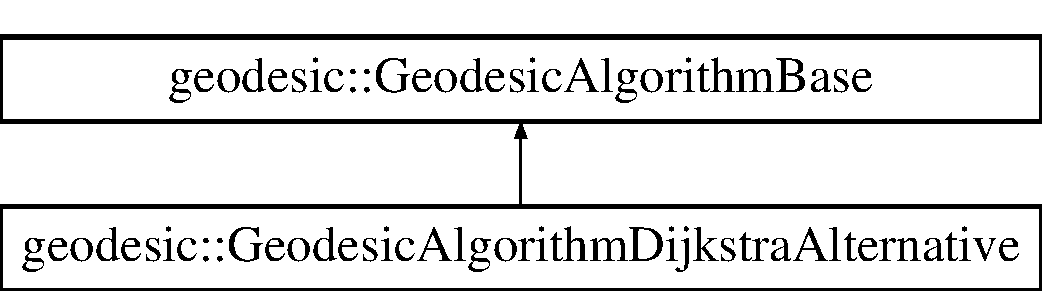
\includegraphics[height=2.000000cm]{classgeodesic_1_1_geodesic_algorithm_dijkstra_alternative}
\end{center}
\end{figure}
\subsection*{Public Types}
\begin{DoxyCompactItemize}
\item 
\hypertarget{classgeodesic_1_1_geodesic_algorithm_dijkstra_alternative_a6cc60d726839ec193d276fa7fe71a8a0}{}typedef \hyperlink{classgeodesic_1_1_dijkstra_node1}{Dijkstra\+Node1} {\bfseries Node}\label{classgeodesic_1_1_geodesic_algorithm_dijkstra_alternative_a6cc60d726839ec193d276fa7fe71a8a0}

\item 
\hypertarget{classgeodesic_1_1_geodesic_algorithm_dijkstra_alternative_a7248597bed80fb5fd1bcd6c794be49c6}{}typedef \hyperlink{classgeodesic_1_1_dijkstra_node1}{Node} $\ast$ {\bfseries node\+\_\+pointer}\label{classgeodesic_1_1_geodesic_algorithm_dijkstra_alternative_a7248597bed80fb5fd1bcd6c794be49c6}

\end{DoxyCompactItemize}
\subsection*{Public Member Functions}
\begin{DoxyCompactItemize}
\item 
\hypertarget{classgeodesic_1_1_geodesic_algorithm_dijkstra_alternative_ae9b9ec8a3dc5a917a871ba74644d6fdc}{}{\bfseries Geodesic\+Algorithm\+Dijkstra\+Alternative} (\hyperlink{classgeodesic_1_1_mesh}{geodesic\+::\+Mesh} $\ast$mesh=N\+U\+L\+L)\label{classgeodesic_1_1_geodesic_algorithm_dijkstra_alternative_ae9b9ec8a3dc5a917a871ba74644d6fdc}

\item 
\hypertarget{classgeodesic_1_1_geodesic_algorithm_dijkstra_alternative_a0e20601049f263d0585311df5faef16f}{}virtual void {\bfseries propagate} (std\+::vector$<$ \hyperlink{classgeodesic_1_1_surface_point}{Surface\+Point} $>$ \&sources, double max\+\_\+propagation\+\_\+distance=G\+E\+O\+D\+E\+S\+I\+C\+\_\+\+I\+N\+F, std\+::vector$<$ \hyperlink{classgeodesic_1_1_surface_point}{Surface\+Point} $>$ $\ast$stop\+\_\+points=N\+U\+L\+L)\label{classgeodesic_1_1_geodesic_algorithm_dijkstra_alternative_a0e20601049f263d0585311df5faef16f}

\item 
\hypertarget{classgeodesic_1_1_geodesic_algorithm_dijkstra_alternative_a2e954bd36a15c007601af006461c34be}{}virtual void {\bfseries trace\+\_\+back} (\hyperlink{classgeodesic_1_1_surface_point}{Surface\+Point} \&destination, std\+::vector$<$ \hyperlink{classgeodesic_1_1_surface_point}{Surface\+Point} $>$ \&path)\label{classgeodesic_1_1_geodesic_algorithm_dijkstra_alternative_a2e954bd36a15c007601af006461c34be}

\item 
\hypertarget{classgeodesic_1_1_geodesic_algorithm_dijkstra_alternative_aaad0321c19c03ccd65cb337247cd524f}{}virtual unsigned {\bfseries best\+\_\+source} (\hyperlink{classgeodesic_1_1_surface_point}{Surface\+Point} \&point, double \&best\+\_\+source\+\_\+distance)\label{classgeodesic_1_1_geodesic_algorithm_dijkstra_alternative_aaad0321c19c03ccd65cb337247cd524f}

\end{DoxyCompactItemize}
\subsection*{Additional Inherited Members}


The documentation for this class was generated from the following file\+:\begin{DoxyCompactItemize}
\item 
src/domain/metric/3rdparty/geodesic/geodesic\+\_\+algorithm\+\_\+dijkstra\+\_\+alternative.\+h\end{DoxyCompactItemize}

\hypertarget{classgeodesic_1_1_geodesic_algorithm_exact}{}\section{geodesic\+:\+:Geodesic\+Algorithm\+Exact Class Reference}
\label{classgeodesic_1_1_geodesic_algorithm_exact}\index{geodesic\+::\+Geodesic\+Algorithm\+Exact@{geodesic\+::\+Geodesic\+Algorithm\+Exact}}
Inheritance diagram for geodesic\+:\+:Geodesic\+Algorithm\+Exact\+:\begin{figure}[H]
\begin{center}
\leavevmode
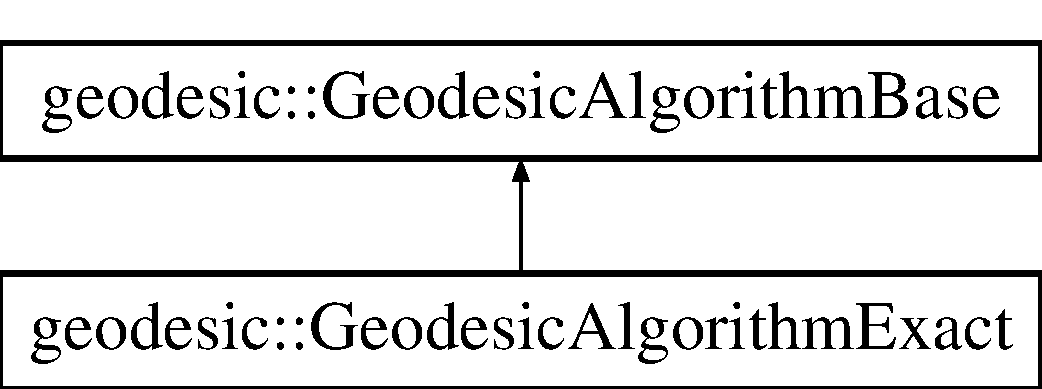
\includegraphics[height=2.000000cm]{classgeodesic_1_1_geodesic_algorithm_exact}
\end{center}
\end{figure}
\subsection*{Public Member Functions}
\begin{DoxyCompactItemize}
\item 
\hypertarget{classgeodesic_1_1_geodesic_algorithm_exact_abaceb49432858b68f283c68b125ca7c0}{}{\bfseries Geodesic\+Algorithm\+Exact} (\hyperlink{classgeodesic_1_1_mesh}{geodesic\+::\+Mesh} $\ast$mesh)\label{classgeodesic_1_1_geodesic_algorithm_exact_abaceb49432858b68f283c68b125ca7c0}

\item 
\hypertarget{classgeodesic_1_1_geodesic_algorithm_exact_afc03c949d24c426e64b30c129715a9bf}{}void {\bfseries propagate} (std\+::vector$<$ \hyperlink{classgeodesic_1_1_surface_point}{Surface\+Point} $>$ \&sources, double max\+\_\+propagation\+\_\+distance=G\+E\+O\+D\+E\+S\+I\+C\+\_\+\+I\+N\+F, std\+::vector$<$ \hyperlink{classgeodesic_1_1_surface_point}{Surface\+Point} $>$ $\ast$stop\+\_\+points=N\+U\+L\+L)\label{classgeodesic_1_1_geodesic_algorithm_exact_afc03c949d24c426e64b30c129715a9bf}

\item 
\hypertarget{classgeodesic_1_1_geodesic_algorithm_exact_a7e261114191fec49e7ae32b8ed53ab21}{}void {\bfseries trace\+\_\+back} (\hyperlink{classgeodesic_1_1_surface_point}{Surface\+Point} \&destination, std\+::vector$<$ \hyperlink{classgeodesic_1_1_surface_point}{Surface\+Point} $>$ \&path)\label{classgeodesic_1_1_geodesic_algorithm_exact_a7e261114191fec49e7ae32b8ed53ab21}

\item 
\hypertarget{classgeodesic_1_1_geodesic_algorithm_exact_a626ac6ed0df6ca0eb8a846659b8dff9b}{}unsigned {\bfseries best\+\_\+source} (\hyperlink{classgeodesic_1_1_surface_point}{Surface\+Point} \&point, double \&best\+\_\+source\+\_\+distance)\label{classgeodesic_1_1_geodesic_algorithm_exact_a626ac6ed0df6ca0eb8a846659b8dff9b}

\item 
\hypertarget{classgeodesic_1_1_geodesic_algorithm_exact_a9ddc832bfa35517cc235180debab3c4d}{}void {\bfseries print\+\_\+statistics} ()\label{classgeodesic_1_1_geodesic_algorithm_exact_a9ddc832bfa35517cc235180debab3c4d}

\end{DoxyCompactItemize}
\subsection*{Additional Inherited Members}


The documentation for this class was generated from the following file\+:\begin{DoxyCompactItemize}
\item 
src/domain/metric/3rdparty/geodesic/geodesic\+\_\+algorithm\+\_\+exact.\+h\end{DoxyCompactItemize}

\hypertarget{classgeodesic_1_1_geodesic_algorithm_graph_base}{}\section{geodesic\+:\+:Geodesic\+Algorithm\+Graph\+Base$<$ Node $>$ Class Template Reference}
\label{classgeodesic_1_1_geodesic_algorithm_graph_base}\index{geodesic\+::\+Geodesic\+Algorithm\+Graph\+Base$<$ Node $>$@{geodesic\+::\+Geodesic\+Algorithm\+Graph\+Base$<$ Node $>$}}
Inheritance diagram for geodesic\+:\+:Geodesic\+Algorithm\+Graph\+Base$<$ Node $>$\+:\begin{figure}[H]
\begin{center}
\leavevmode
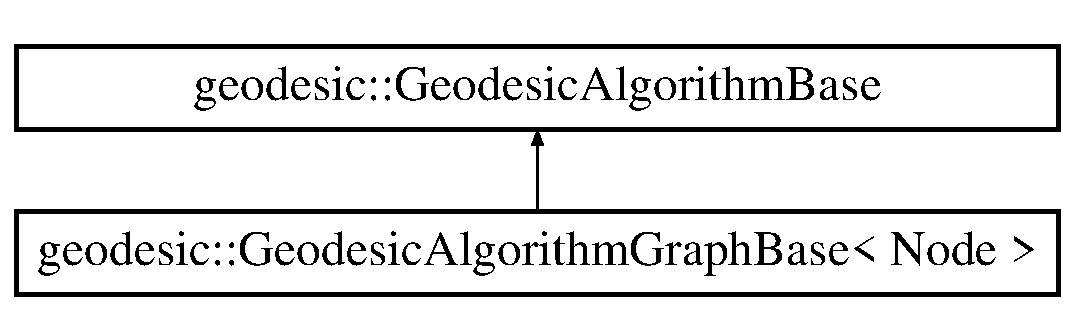
\includegraphics[height=2.000000cm]{classgeodesic_1_1_geodesic_algorithm_graph_base}
\end{center}
\end{figure}
\subsection*{Public Types}
\begin{DoxyCompactItemize}
\item 
\hypertarget{classgeodesic_1_1_geodesic_algorithm_graph_base_a0926f4142d3390c5e3555163f6b6a2d9}{}typedef Node $\ast$ {\bfseries node\+\_\+pointer}\label{classgeodesic_1_1_geodesic_algorithm_graph_base_a0926f4142d3390c5e3555163f6b6a2d9}

\end{DoxyCompactItemize}
\subsection*{Public Member Functions}
\begin{DoxyCompactItemize}
\item 
\hypertarget{classgeodesic_1_1_geodesic_algorithm_graph_base_ae492310ecfd6208a727d1680d9751179}{}{\bfseries Geodesic\+Algorithm\+Graph\+Base} (\hyperlink{classgeodesic_1_1_mesh}{geodesic\+::\+Mesh} $\ast$mesh)\label{classgeodesic_1_1_geodesic_algorithm_graph_base_ae492310ecfd6208a727d1680d9751179}

\item 
\hypertarget{classgeodesic_1_1_geodesic_algorithm_graph_base_a626631f58f33d7e53f3e68f5851d7808}{}void {\bfseries propagate} (std\+::vector$<$ \hyperlink{classgeodesic_1_1_surface_point}{Surface\+Point} $>$ \&sources, double max\+\_\+propagation\+\_\+distance=G\+E\+O\+D\+E\+S\+I\+C\+\_\+\+I\+N\+F, std\+::vector$<$ \hyperlink{classgeodesic_1_1_surface_point}{Surface\+Point} $>$ $\ast$stop\+\_\+points=N\+U\+L\+L)\label{classgeodesic_1_1_geodesic_algorithm_graph_base_a626631f58f33d7e53f3e68f5851d7808}

\item 
\hypertarget{classgeodesic_1_1_geodesic_algorithm_graph_base_a8166429fb5f94a4654a8ff3db1712aea}{}void {\bfseries trace\+\_\+back} (\hyperlink{classgeodesic_1_1_surface_point}{Surface\+Point} \&destination, std\+::vector$<$ \hyperlink{classgeodesic_1_1_surface_point}{Surface\+Point} $>$ \&path)\label{classgeodesic_1_1_geodesic_algorithm_graph_base_a8166429fb5f94a4654a8ff3db1712aea}

\item 
\hypertarget{classgeodesic_1_1_geodesic_algorithm_graph_base_aef5dc1c15289e879166f0b8f378772b5}{}unsigned {\bfseries best\+\_\+source} (\hyperlink{classgeodesic_1_1_surface_point}{Surface\+Point} \&point, double \&best\+\_\+source\+\_\+distance)\label{classgeodesic_1_1_geodesic_algorithm_graph_base_aef5dc1c15289e879166f0b8f378772b5}

\item 
\hypertarget{classgeodesic_1_1_geodesic_algorithm_graph_base_a0254b8c4e9ec6bafcf4ab78fb2867a80}{}void {\bfseries print\+\_\+statistics} ()\label{classgeodesic_1_1_geodesic_algorithm_graph_base_a0254b8c4e9ec6bafcf4ab78fb2867a80}

\end{DoxyCompactItemize}
\subsection*{Protected Types}
\begin{DoxyCompactItemize}
\item 
\hypertarget{classgeodesic_1_1_geodesic_algorithm_graph_base_a83b12ebf237e79081ad75397f2b9238d}{}typedef std\+::set$<$ node\+\_\+pointer, Node $>$ {\bfseries queue\+\_\+type}\label{classgeodesic_1_1_geodesic_algorithm_graph_base_a83b12ebf237e79081ad75397f2b9238d}

\end{DoxyCompactItemize}
\subsection*{Protected Member Functions}
\begin{DoxyCompactItemize}
\item 
\hypertarget{classgeodesic_1_1_geodesic_algorithm_graph_base_ad07e47e87272d4d7a754da85b232d94f}{}unsigned {\bfseries node\+\_\+index} (\hyperlink{classgeodesic_1_1_vertex}{vertex\+\_\+pointer} v)\label{classgeodesic_1_1_geodesic_algorithm_graph_base_ad07e47e87272d4d7a754da85b232d94f}

\item 
\hypertarget{classgeodesic_1_1_geodesic_algorithm_graph_base_a63974d998001f79edd6e157cceffe977}{}void {\bfseries set\+\_\+sources} (std\+::vector$<$ \hyperlink{classgeodesic_1_1_surface_point}{Surface\+Point} $>$ \&sources)\label{classgeodesic_1_1_geodesic_algorithm_graph_base_a63974d998001f79edd6e157cceffe977}

\item 
\hypertarget{classgeodesic_1_1_geodesic_algorithm_graph_base_a4a0ce4a71cecefd2005173da1c5065a3}{}node\+\_\+pointer {\bfseries best\+\_\+first\+\_\+node} (\hyperlink{classgeodesic_1_1_surface_point}{Surface\+Point} \&point, double \&best\+\_\+total\+\_\+distance)\label{classgeodesic_1_1_geodesic_algorithm_graph_base_a4a0ce4a71cecefd2005173da1c5065a3}

\item 
\hypertarget{classgeodesic_1_1_geodesic_algorithm_graph_base_a74c976177590a38dc876fb9ac0a037b2}{}bool {\bfseries check\+\_\+stop\+\_\+conditions} (unsigned \&index)\label{classgeodesic_1_1_geodesic_algorithm_graph_base_a74c976177590a38dc876fb9ac0a037b2}

\item 
\hypertarget{classgeodesic_1_1_geodesic_algorithm_graph_base_ab3898bf1b1c480ecb93e9ecdbb4ae0b8}{}virtual void {\bfseries list\+\_\+nodes\+\_\+visible\+\_\+from\+\_\+source} (\hyperlink{classgeodesic_1_1_mesh_element_base}{Mesh\+Element\+Base} $\ast$p, std\+::vector$<$ node\+\_\+pointer $>$ \&storage)=0\label{classgeodesic_1_1_geodesic_algorithm_graph_base_ab3898bf1b1c480ecb93e9ecdbb4ae0b8}

\item 
\hypertarget{classgeodesic_1_1_geodesic_algorithm_graph_base_a86446e8b1c9938016119ccd794be4882}{}virtual void {\bfseries list\+\_\+nodes\+\_\+visible\+\_\+from\+\_\+node} (node\+\_\+pointer node, std\+::vector$<$ node\+\_\+pointer $>$ \&storage, std\+::vector$<$ double $>$ \&distances, double threshold\+\_\+distance)=0\label{classgeodesic_1_1_geodesic_algorithm_graph_base_a86446e8b1c9938016119ccd794be4882}

\end{DoxyCompactItemize}
\subsection*{Protected Attributes}
\begin{DoxyCompactItemize}
\item 
\hypertarget{classgeodesic_1_1_geodesic_algorithm_graph_base_a33b2fc3faa40d7fa2df9873803274013}{}std\+::vector$<$ Node $>$ {\bfseries m\+\_\+nodes}\label{classgeodesic_1_1_geodesic_algorithm_graph_base_a33b2fc3faa40d7fa2df9873803274013}

\item 
\hypertarget{classgeodesic_1_1_geodesic_algorithm_graph_base_a295cc419900e077f47719064690dac5d}{}queue\+\_\+type {\bfseries m\+\_\+queue}\label{classgeodesic_1_1_geodesic_algorithm_graph_base_a295cc419900e077f47719064690dac5d}

\item 
\hypertarget{classgeodesic_1_1_geodesic_algorithm_graph_base_aa48d0a59f9f4983571adb39813a337ae}{}std\+::vector$<$ \hyperlink{classgeodesic_1_1_surface_point}{Surface\+Point} $>$ {\bfseries m\+\_\+sources}\label{classgeodesic_1_1_geodesic_algorithm_graph_base_aa48d0a59f9f4983571adb39813a337ae}

\end{DoxyCompactItemize}


The documentation for this class was generated from the following file\+:\begin{DoxyCompactItemize}
\item 
src/domain/metric/3rdparty/geodesic/geodesic\+\_\+algorithm\+\_\+graph\+\_\+base.\+h\end{DoxyCompactItemize}

\hypertarget{classgeodesic_1_1_geodesic_algorithm_subdivision}{}\section{geodesic\+:\+:Geodesic\+Algorithm\+Subdivision Class Reference}
\label{classgeodesic_1_1_geodesic_algorithm_subdivision}\index{geodesic\+::\+Geodesic\+Algorithm\+Subdivision@{geodesic\+::\+Geodesic\+Algorithm\+Subdivision}}
Inheritance diagram for geodesic\+:\+:Geodesic\+Algorithm\+Subdivision\+:\begin{figure}[H]
\begin{center}
\leavevmode
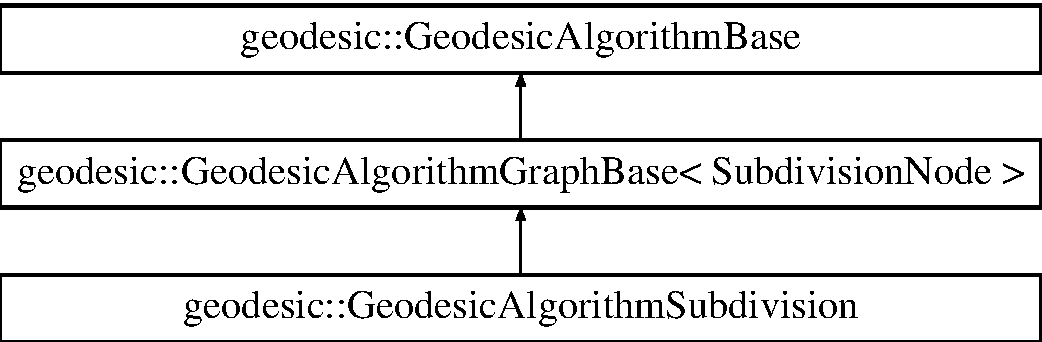
\includegraphics[height=3.000000cm]{classgeodesic_1_1_geodesic_algorithm_subdivision}
\end{center}
\end{figure}
\subsection*{Public Member Functions}
\begin{DoxyCompactItemize}
\item 
\hyperlink{classgeodesic_1_1_geodesic_algorithm_subdivision_a72dacc31bf5f71a59ab7af93d9f798a9}{Geodesic\+Algorithm\+Subdivision} (\hyperlink{classgeodesic_1_1_mesh}{geodesic\+::\+Mesh} $\ast$mesh=N\+U\+L\+L, unsigned subdivision\+\_\+level=0)
\item 
\hypertarget{classgeodesic_1_1_geodesic_algorithm_subdivision_aad6c35c368039996b56bd119f6053731}{}unsigned {\bfseries subdivision\+\_\+level} ()\label{classgeodesic_1_1_geodesic_algorithm_subdivision_aad6c35c368039996b56bd119f6053731}

\item 
\hypertarget{classgeodesic_1_1_geodesic_algorithm_subdivision_a3af97fcc59f11dc2eed03e9b83e0c91a}{}void {\bfseries set\+\_\+subdivision\+\_\+level} (unsigned subdivision\+\_\+level)\label{classgeodesic_1_1_geodesic_algorithm_subdivision_a3af97fcc59f11dc2eed03e9b83e0c91a}

\end{DoxyCompactItemize}
\subsection*{Protected Member Functions}
\begin{DoxyCompactItemize}
\item 
\hypertarget{classgeodesic_1_1_geodesic_algorithm_subdivision_ac48be36945b8d18a28cafa0a45bcdf75}{}void {\bfseries list\+\_\+nodes\+\_\+visible\+\_\+from\+\_\+source} (\hyperlink{classgeodesic_1_1_mesh_element_base}{Mesh\+Element\+Base} $\ast$p, std\+::vector$<$ \hyperlink{classgeodesic_1_1_subdivision_node}{node\+\_\+pointer} $>$ \&storage)\label{classgeodesic_1_1_geodesic_algorithm_subdivision_ac48be36945b8d18a28cafa0a45bcdf75}

\item 
\hypertarget{classgeodesic_1_1_geodesic_algorithm_subdivision_a35c3361a19ac215d890a8e51e31f0ca4}{}void {\bfseries list\+\_\+nodes\+\_\+visible\+\_\+from\+\_\+node} (\hyperlink{classgeodesic_1_1_subdivision_node}{node\+\_\+pointer} node, std\+::vector$<$ \hyperlink{classgeodesic_1_1_subdivision_node}{node\+\_\+pointer} $>$ \&storage, std\+::vector$<$ double $>$ \&distances, double threshold\+\_\+distance)\label{classgeodesic_1_1_geodesic_algorithm_subdivision_a35c3361a19ac215d890a8e51e31f0ca4}

\item 
\hypertarget{classgeodesic_1_1_geodesic_algorithm_subdivision_a963cf8fddfb3a934be163e4db979ea65}{}unsigned {\bfseries node\+\_\+indexx} (\hyperlink{classgeodesic_1_1_edge}{edge\+\_\+pointer} e)\label{classgeodesic_1_1_geodesic_algorithm_subdivision_a963cf8fddfb3a934be163e4db979ea65}

\end{DoxyCompactItemize}
\subsection*{Additional Inherited Members}


\subsection{Constructor \& Destructor Documentation}
\hypertarget{classgeodesic_1_1_geodesic_algorithm_subdivision_a72dacc31bf5f71a59ab7af93d9f798a9}{}\index{geodesic\+::\+Geodesic\+Algorithm\+Subdivision@{geodesic\+::\+Geodesic\+Algorithm\+Subdivision}!Geodesic\+Algorithm\+Subdivision@{Geodesic\+Algorithm\+Subdivision}}
\index{Geodesic\+Algorithm\+Subdivision@{Geodesic\+Algorithm\+Subdivision}!geodesic\+::\+Geodesic\+Algorithm\+Subdivision@{geodesic\+::\+Geodesic\+Algorithm\+Subdivision}}
\subsubsection[{Geodesic\+Algorithm\+Subdivision}]{\setlength{\rightskip}{0pt plus 5cm}geodesic\+::\+Geodesic\+Algorithm\+Subdivision\+::\+Geodesic\+Algorithm\+Subdivision (
\begin{DoxyParamCaption}
\item[{{\bf geodesic\+::\+Mesh} $\ast$}]{mesh = {\ttfamily NULL}, }
\item[{unsigned}]{subdivision\+\_\+level = {\ttfamily 0}}
\end{DoxyParamCaption}
)\hspace{0.3cm}{\ttfamily [inline]}}\label{classgeodesic_1_1_geodesic_algorithm_subdivision_a72dacc31bf5f71a59ab7af93d9f798a9}
! 

The documentation for this class was generated from the following file\+:\begin{DoxyCompactItemize}
\item 
src/domain/metric/3rdparty/geodesic/geodesic\+\_\+algorithm\+\_\+subdivision.\+h\end{DoxyCompactItemize}

\hypertarget{class_geodesic_metric}{}\section{Geodesic\+Metric Class Reference}
\label{class_geodesic_metric}\index{Geodesic\+Metric@{Geodesic\+Metric}}
Inheritance diagram for Geodesic\+Metric\+:\begin{figure}[H]
\begin{center}
\leavevmode
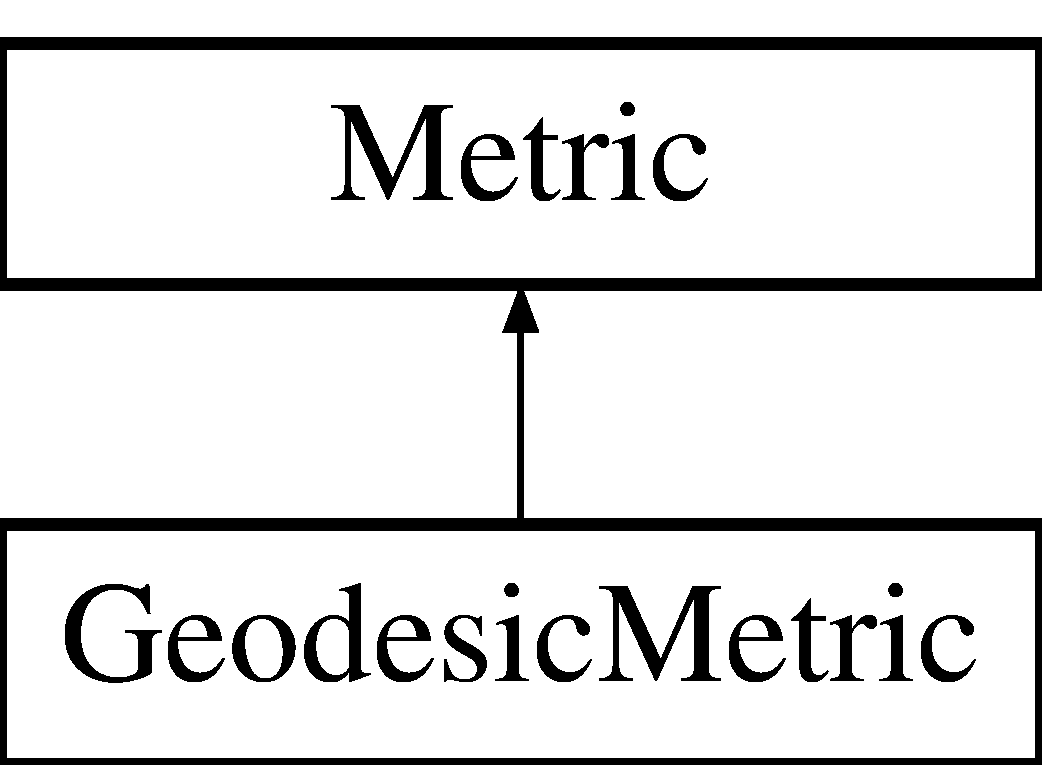
\includegraphics[height=2.000000cm]{class_geodesic_metric}
\end{center}
\end{figure}
\subsection*{Public Member Functions}
\begin{DoxyCompactItemize}
\item 
\hypertarget{class_geodesic_metric_abf3bc74380d3bc25428e1f18e635ff92}{}virtual void {\bfseries initialize} (\hyperlink{class_shape}{Shape} $\ast$shape)\label{class_geodesic_metric_abf3bc74380d3bc25428e1f18e635ff92}

\item 
\hypertarget{class_geodesic_metric_a654c8a9b8b6a091134b4108c619ccc91}{}virtual double {\bfseries get\+Distance} (vtk\+Id\+Type a, vtk\+Id\+Type b)\label{class_geodesic_metric_a654c8a9b8b6a091134b4108c619ccc91}

\item 
\hypertarget{class_geodesic_metric_aff4a4dc1b147c31c074262e89d412ec4}{}virtual void {\bfseries get\+All\+Distances} (\hyperlink{class_scalar_point_attribute}{Scalar\+Point\+Attribute} \&distances, vtk\+Id\+Type source)\label{class_geodesic_metric_aff4a4dc1b147c31c074262e89d412ec4}

\item 
\hypertarget{class_geodesic_metric_a1cd4191f24b7e5e06aec166db9e26b6c}{}virtual vtk\+Smart\+Pointer$<$ vtk\+Id\+List $>$ {\bfseries get\+Voronoi\+Cells} (vtk\+Smart\+Pointer$<$ vtk\+Id\+List $>$ seeds)\label{class_geodesic_metric_a1cd4191f24b7e5e06aec166db9e26b6c}

\item 
\hypertarget{class_geodesic_metric_a7215349bd977395f2dd27c6a6b5959bf}{}virtual vtk\+Id\+Type {\bfseries get\+Farthest\+Point} (vtk\+Smart\+Pointer$<$ vtk\+Id\+List $>$ sources)\label{class_geodesic_metric_a7215349bd977395f2dd27c6a6b5959bf}

\end{DoxyCompactItemize}
\subsection*{Static Public Member Functions}
\begin{DoxyCompactItemize}
\item 
\hypertarget{class_geodesic_metric_a389074cfb665370b570fd57f7ab83df8}{}static \hyperlink{class_metric}{Metric} $\ast$ {\bfseries create} ()\label{class_geodesic_metric_a389074cfb665370b570fd57f7ab83df8}

\item 
\hypertarget{class_geodesic_metric_ad0a874b2bc7f683685add0e1049361ab}{}static string {\bfseries get\+Identifier} ()\label{class_geodesic_metric_ad0a874b2bc7f683685add0e1049361ab}

\end{DoxyCompactItemize}
\subsection*{Additional Inherited Members}


The documentation for this class was generated from the following files\+:\begin{DoxyCompactItemize}
\item 
src/domain/metric/Geodesic\+Metric.\+h\item 
src/domain/metric/Geodesic\+Metric.\+cpp\end{DoxyCompactItemize}

\hypertarget{class_global_point_signature}{}\section{Global\+Point\+Signature Class Reference}
\label{class_global_point_signature}\index{Global\+Point\+Signature@{Global\+Point\+Signature}}
Inheritance diagram for Global\+Point\+Signature\+:\begin{figure}[H]
\begin{center}
\leavevmode
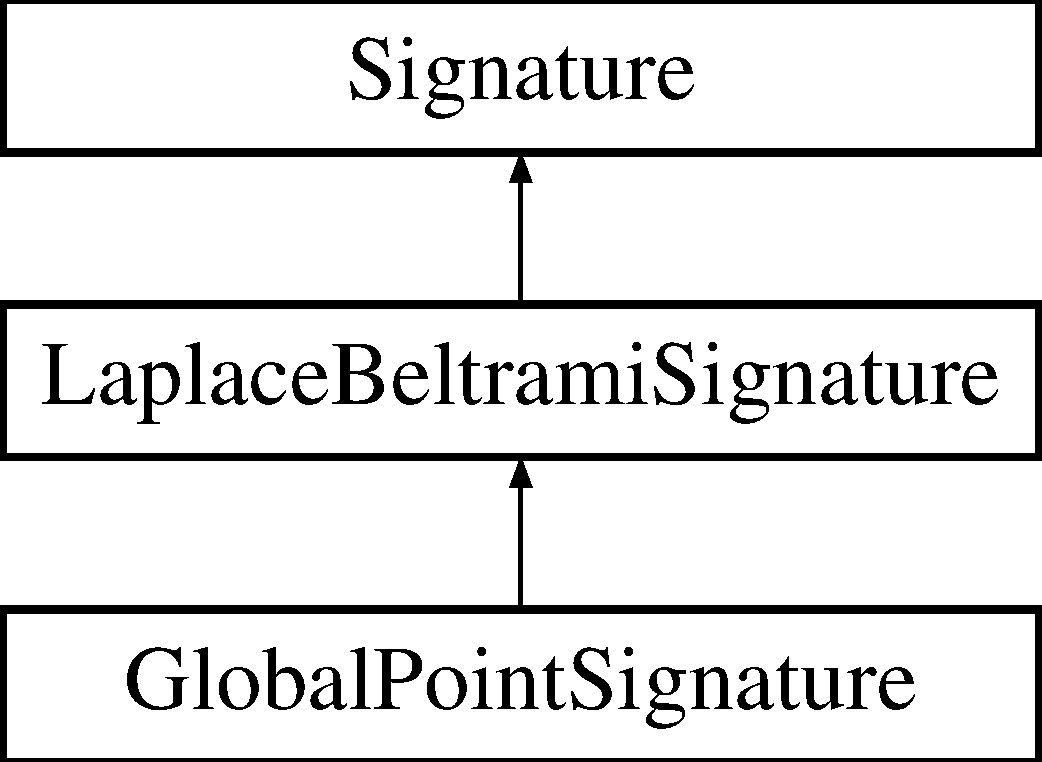
\includegraphics[height=3.000000cm]{class_global_point_signature}
\end{center}
\end{figure}
\subsection*{Public Member Functions}
\begin{DoxyCompactItemize}
\item 
\hypertarget{class_global_point_signature_a4850302ad29f52fcaaf53dd897e87be7}{}virtual void {\bfseries initialize} (\hyperlink{class_shape}{Shape} $\ast$shape, int dimension)\label{class_global_point_signature_a4850302ad29f52fcaaf53dd897e87be7}

\end{DoxyCompactItemize}
\subsection*{Static Public Member Functions}
\begin{DoxyCompactItemize}
\item 
\hypertarget{class_global_point_signature_a3d48915c2cf9cfffc26a1574d2168fdb}{}static \hyperlink{class_laplace_beltrami_signature}{Laplace\+Beltrami\+Signature} $\ast$ {\bfseries create} ()\label{class_global_point_signature_a3d48915c2cf9cfffc26a1574d2168fdb}

\item 
\hypertarget{class_global_point_signature_a2e19188d72e93581e5826e7f35a43be8}{}static string {\bfseries get\+Identifier} ()\label{class_global_point_signature_a2e19188d72e93581e5826e7f35a43be8}

\end{DoxyCompactItemize}
\subsection*{Additional Inherited Members}


The documentation for this class was generated from the following files\+:\begin{DoxyCompactItemize}
\item 
src/domain/signatures/Global\+Point\+Signature.\+h\item 
src/domain/signatures/Global\+Point\+Signature.\+cpp\end{DoxyCompactItemize}

\hypertarget{structgeodesic_1_1_half_edge}{}\section{geodesic\+:\+:Half\+Edge Struct Reference}
\label{structgeodesic_1_1_half_edge}\index{geodesic\+::\+Half\+Edge@{geodesic\+::\+Half\+Edge}}
\subsection*{Public Attributes}
\begin{DoxyCompactItemize}
\item 
\hypertarget{structgeodesic_1_1_half_edge_a82a852c100d5a90b002d5b111c97c31e}{}unsigned {\bfseries face\+\_\+id}\label{structgeodesic_1_1_half_edge_a82a852c100d5a90b002d5b111c97c31e}

\item 
\hypertarget{structgeodesic_1_1_half_edge_ae94938b088eb133f9073bb81a58665dd}{}unsigned {\bfseries vertex\+\_\+0}\label{structgeodesic_1_1_half_edge_ae94938b088eb133f9073bb81a58665dd}

\item 
\hypertarget{structgeodesic_1_1_half_edge_a5cae2651ffb17ca758174c740f56a1d6}{}unsigned {\bfseries vertex\+\_\+1}\label{structgeodesic_1_1_half_edge_a5cae2651ffb17ca758174c740f56a1d6}

\end{DoxyCompactItemize}


The documentation for this struct was generated from the following file\+:\begin{DoxyCompactItemize}
\item 
src/domain/metric/3rdparty/geodesic/geodesic\+\_\+mesh\+\_\+elements.\+h\end{DoxyCompactItemize}

\hypertarget{class_hash_map}{}\section{Hash\+Map$<$ K\+E\+Y, V\+A\+L\+U\+E $>$ Class Template Reference}
\label{class_hash_map}\index{Hash\+Map$<$ K\+E\+Y, V\+A\+L\+U\+E $>$@{Hash\+Map$<$ K\+E\+Y, V\+A\+L\+U\+E $>$}}
\subsection*{Public Types}
\begin{DoxyCompactItemize}
\item 
\hypertarget{class_hash_map_a0253297a2d2712a409956b0cfd3ac717}{}typedef unordered\+\_\+map$<$ K\+E\+Y, V\+A\+L\+U\+E $>$\+::iterator {\bfseries iterator}\label{class_hash_map_a0253297a2d2712a409956b0cfd3ac717}

\end{DoxyCompactItemize}
\subsection*{Public Member Functions}
\begin{DoxyCompactItemize}
\item 
bool \hyperlink{class_hash_map_a7391f737a46c640dde378655e347727f}{contains\+Key} (K\+E\+Y)
\begin{DoxyCompactList}\small\item\em Returns if the given key exists in the hash map. \end{DoxyCompactList}\item 
V\+A\+L\+U\+E \& \hyperlink{class_hash_map_aaf70432c8b6cf09fb8024cd402d1bd7c}{operator\mbox{[}$\,$\mbox{]}} (K\+E\+Y)
\begin{DoxyCompactList}\small\item\em Returns the value corresponding to the key. \end{DoxyCompactList}\item 
\hypertarget{class_hash_map_ae29dc2b5b58f05690e455a51aeb7341d}{}unsigned \hyperlink{class_hash_map_ae29dc2b5b58f05690e455a51aeb7341d}{size} ()\label{class_hash_map_ae29dc2b5b58f05690e455a51aeb7341d}

\begin{DoxyCompactList}\small\item\em Returns the number of elements in the hash map. \end{DoxyCompactList}\item 
void \hyperlink{class_hash_map_a48a73346ed336eaaabbc23ac610b67a1}{get\+Random\+Sample} (unsigned \hyperlink{class_hash_map_ae29dc2b5b58f05690e455a51aeb7341d}{size}, \hyperlink{class_hash_map}{Hash\+Map}$<$ K\+E\+Y, V\+A\+L\+U\+E $>$ \&hashmap)
\begin{DoxyCompactList}\small\item\em Stores a random subset of size 'size' in the given hash map. \end{DoxyCompactList}\item 
void \hyperlink{class_hash_map_a8d0dade42862374087389ca082025165}{get\+Random\+Sample\+Keys} (unsigned \hyperlink{class_hash_map_ae29dc2b5b58f05690e455a51aeb7341d}{size}, vector$<$ K\+E\+Y $>$ \&vector)
\begin{DoxyCompactList}\small\item\em Stores a random subset of size 'size' of the keys in the given vector. \end{DoxyCompactList}\item 
void \hyperlink{class_hash_map_a8babe9098191e29b4fb10f1b8f1427d5}{get\+Random\+Sample\+Values} (unsigned \hyperlink{class_hash_map_ae29dc2b5b58f05690e455a51aeb7341d}{size}, vector$<$ V\+A\+L\+U\+E $>$ \&vector)
\begin{DoxyCompactList}\small\item\em Stores a random subset of size 'size' of the values in the given vector. \end{DoxyCompactList}\item 
\hypertarget{class_hash_map_a68db9203d908598b70b8325194c54819}{}unordered\+\_\+map$<$ K\+E\+Y, V\+A\+L\+U\+E $>$ \& \hyperlink{class_hash_map_a68db9203d908598b70b8325194c54819}{get\+Entries} ()\label{class_hash_map_a68db9203d908598b70b8325194c54819}

\begin{DoxyCompactList}\small\item\em Returns a pointer to the unordered\+\_\+map. \end{DoxyCompactList}\item 
void \hyperlink{class_hash_map_abc87b6932fa1319156a3d5fa9c46a446}{get\+Values} (vector$<$ V\+A\+L\+U\+E $>$ \&)
\begin{DoxyCompactList}\small\item\em Stores all values in the given vector. \end{DoxyCompactList}\item 
\hypertarget{class_hash_map_ab7f911839bbe21bf582a8b69c9f500d1}{}void \hyperlink{class_hash_map_ab7f911839bbe21bf582a8b69c9f500d1}{get\+Keys} (vector$<$ K\+E\+Y $>$ \&)\label{class_hash_map_ab7f911839bbe21bf582a8b69c9f500d1}

\begin{DoxyCompactList}\small\item\em Stores all keys in the given vector. \end{DoxyCompactList}\end{DoxyCompactItemize}
{\bf }\par
\begin{DoxyCompactItemize}
\item 
\hypertarget{class_hash_map_ace56e25bbddde14be403a9b2224dd364}{}\hyperlink{class_hash_map_ace56e25bbddde14be403a9b2224dd364}{Hash\+Map} ()\label{class_hash_map_ace56e25bbddde14be403a9b2224dd364}

\begin{DoxyCompactList}\small\item\em Empty Constructor. \end{DoxyCompactList}\item 
\hypertarget{class_hash_map_a921ee1145e96f83f3776f0100b8f7275}{}\hyperlink{class_hash_map_a921ee1145e96f83f3776f0100b8f7275}{Hash\+Map} (int n)\label{class_hash_map_a921ee1145e96f83f3776f0100b8f7275}

\begin{DoxyCompactList}\small\item\em Reserves memory for n elements. \end{DoxyCompactList}\item 
\hypertarget{class_hash_map_a2a86d581bca37b123a56f1198337a792}{}\hyperlink{class_hash_map_a2a86d581bca37b123a56f1198337a792}{Hash\+Map} (\hyperlink{class_hash_map}{Hash\+Map}$<$ K\+E\+Y, V\+A\+L\+U\+E $>$ \&)\label{class_hash_map_a2a86d581bca37b123a56f1198337a792}

\begin{DoxyCompactList}\small\item\em Copy Constructor. \end{DoxyCompactList}\item 
\hypertarget{class_hash_map_a65b3b62f510bb745a886ef7e9618324c}{}\hyperlink{class_hash_map_a65b3b62f510bb745a886ef7e9618324c}{Hash\+Map} (vector$<$ K\+E\+Y $>$ \&, V\+A\+L\+U\+E)\label{class_hash_map_a65b3b62f510bb745a886ef7e9618324c}

\begin{DoxyCompactList}\small\item\em Maps all keys to the given value. \end{DoxyCompactList}\item 
\hypertarget{class_hash_map_a92ad972027e37d1d8f3d311a441190fc}{}\hyperlink{class_hash_map_a92ad972027e37d1d8f3d311a441190fc}{$\sim$\+Hash\+Map} ()\label{class_hash_map_a92ad972027e37d1d8f3d311a441190fc}

\begin{DoxyCompactList}\small\item\em Empty Destructor. \end{DoxyCompactList}\end{DoxyCompactItemize}

{\bf }\par
\begin{DoxyCompactItemize}
\item 
void \hyperlink{class_hash_map_a6c177f77bc0b96cd6c6c1601b3e0714e}{add} (K\+E\+Y, V\+A\+L\+U\+E)
\begin{DoxyCompactList}\small\item\em Adds the value with the given key. \end{DoxyCompactList}\item 
void \hyperlink{class_hash_map_a8178f15b99b857b84ea88ebabf4fe53b}{add} (vector$<$ K\+E\+Y $>$ \&, V\+A\+L\+U\+E)
\begin{DoxyCompactList}\small\item\em Maps all given keys to the given value. \end{DoxyCompactList}\item 
void \hyperlink{class_hash_map_ac56f67e281f1bd91539035535c815121}{add} (vector$<$ pair$<$ K\+E\+Y, V\+A\+L\+U\+E $>$ $>$ \&)
\begin{DoxyCompactList}\small\item\em Adds all key, value pairs. \end{DoxyCompactList}\end{DoxyCompactItemize}

{\bf }\par
\begin{DoxyCompactItemize}
\item 
\hypertarget{class_hash_map_a0cc42915eadab1175b35cbee6cd658c1}{}bool \hyperlink{class_hash_map_a0cc42915eadab1175b35cbee6cd658c1}{remove} (K\+E\+Y)\label{class_hash_map_a0cc42915eadab1175b35cbee6cd658c1}

\begin{DoxyCompactList}\small\item\em If the key exists, its corresponding value is removed from the hash map. \end{DoxyCompactList}\item 
\hypertarget{class_hash_map_ac1997800708d2723afba29bbd4d494bf}{}bool \hyperlink{class_hash_map_ac1997800708d2723afba29bbd4d494bf}{remove} (vector$<$ K\+E\+Y $>$ \&)\label{class_hash_map_ac1997800708d2723afba29bbd4d494bf}

\begin{DoxyCompactList}\small\item\em Calls \hyperlink{class_hash_map_a0cc42915eadab1175b35cbee6cd658c1}{remove(\+K\+E\+Y)} on every element in the vector. \end{DoxyCompactList}\item 
\hypertarget{class_hash_map_aa63e547f51d713c06d7e70c0a3fc23ad}{}void \hyperlink{class_hash_map_aa63e547f51d713c06d7e70c0a3fc23ad}{clear} ()\label{class_hash_map_aa63e547f51d713c06d7e70c0a3fc23ad}

\begin{DoxyCompactList}\small\item\em Clears the whole hash map. \end{DoxyCompactList}\end{DoxyCompactItemize}

{\bf }\par
\begin{DoxyCompactItemize}
\item 
\hypertarget{class_hash_map_a3b0a486bb4e801097ebb7fd40282a513}{}iterator \hyperlink{class_hash_map_a3b0a486bb4e801097ebb7fd40282a513}{begin} ()\label{class_hash_map_a3b0a486bb4e801097ebb7fd40282a513}

\begin{DoxyCompactList}\small\item\em Returns iterator pointing to the first element of the hashmap. \end{DoxyCompactList}\item 
\hypertarget{class_hash_map_a37735a61fd58501770200671497f9388}{}iterator \hyperlink{class_hash_map_a37735a61fd58501770200671497f9388}{end} ()\label{class_hash_map_a37735a61fd58501770200671497f9388}

\begin{DoxyCompactList}\small\item\em Returns iterator pointing to the end of the hash map. \end{DoxyCompactList}\end{DoxyCompactItemize}



\subsection{Member Function Documentation}
\hypertarget{class_hash_map_a6c177f77bc0b96cd6c6c1601b3e0714e}{}\index{Hash\+Map@{Hash\+Map}!add@{add}}
\index{add@{add}!Hash\+Map@{Hash\+Map}}
\subsubsection[{add}]{\setlength{\rightskip}{0pt plus 5cm}template$<$class K\+E\+Y, class V\+A\+L\+U\+E$>$ void {\bf Hash\+Map}$<$ K\+E\+Y, V\+A\+L\+U\+E $>$\+::add (
\begin{DoxyParamCaption}
\item[{K\+E\+Y}]{key, }
\item[{V\+A\+L\+U\+E}]{value}
\end{DoxyParamCaption}
)}\label{class_hash_map_a6c177f77bc0b96cd6c6c1601b3e0714e}


Adds the value with the given key. 

If the key already exists the corresponding value is replaced. \hypertarget{class_hash_map_a8178f15b99b857b84ea88ebabf4fe53b}{}\index{Hash\+Map@{Hash\+Map}!add@{add}}
\index{add@{add}!Hash\+Map@{Hash\+Map}}
\subsubsection[{add}]{\setlength{\rightskip}{0pt plus 5cm}template$<$class K\+E\+Y, class V\+A\+L\+U\+E$>$ void {\bf Hash\+Map}$<$ K\+E\+Y, V\+A\+L\+U\+E $>$\+::add (
\begin{DoxyParamCaption}
\item[{vector$<$ K\+E\+Y $>$ \&}]{keys, }
\item[{V\+A\+L\+U\+E}]{value}
\end{DoxyParamCaption}
)}\label{class_hash_map_a8178f15b99b857b84ea88ebabf4fe53b}


Maps all given keys to the given value. 

If any of the keys already exist the corresponding value is replaced. \hypertarget{class_hash_map_ac56f67e281f1bd91539035535c815121}{}\index{Hash\+Map@{Hash\+Map}!add@{add}}
\index{add@{add}!Hash\+Map@{Hash\+Map}}
\subsubsection[{add}]{\setlength{\rightskip}{0pt plus 5cm}template$<$class K\+E\+Y, class V\+A\+L\+U\+E$>$ void {\bf Hash\+Map}$<$ K\+E\+Y, V\+A\+L\+U\+E $>$\+::add (
\begin{DoxyParamCaption}
\item[{vector$<$ pair$<$ K\+E\+Y, V\+A\+L\+U\+E $>$ $>$ \&}]{entries}
\end{DoxyParamCaption}
)}\label{class_hash_map_ac56f67e281f1bd91539035535c815121}


Adds all key, value pairs. 

If any of the keys already exist the corresponding value is replaced. \hypertarget{class_hash_map_a7391f737a46c640dde378655e347727f}{}\index{Hash\+Map@{Hash\+Map}!contains\+Key@{contains\+Key}}
\index{contains\+Key@{contains\+Key}!Hash\+Map@{Hash\+Map}}
\subsubsection[{contains\+Key}]{\setlength{\rightskip}{0pt plus 5cm}template$<$class K\+E\+Y, class V\+A\+L\+U\+E $>$ bool {\bf Hash\+Map}$<$ K\+E\+Y, V\+A\+L\+U\+E $>$\+::contains\+Key (
\begin{DoxyParamCaption}
\item[{K\+E\+Y}]{key}
\end{DoxyParamCaption}
)}\label{class_hash_map_a7391f737a46c640dde378655e347727f}


Returns if the given key exists in the hash map. 

This will not cause the key to be added to the hash map. \begin{DoxyReturn}{Returns}
true if key exists, false otherwise 
\end{DoxyReturn}
\hypertarget{class_hash_map_a48a73346ed336eaaabbc23ac610b67a1}{}\index{Hash\+Map@{Hash\+Map}!get\+Random\+Sample@{get\+Random\+Sample}}
\index{get\+Random\+Sample@{get\+Random\+Sample}!Hash\+Map@{Hash\+Map}}
\subsubsection[{get\+Random\+Sample}]{\setlength{\rightskip}{0pt plus 5cm}template$<$class K\+E\+Y, class V\+A\+L\+U\+E$>$ void {\bf Hash\+Map}$<$ K\+E\+Y, V\+A\+L\+U\+E $>$\+::get\+Random\+Sample (
\begin{DoxyParamCaption}
\item[{unsigned}]{size, }
\item[{{\bf Hash\+Map}$<$ K\+E\+Y, V\+A\+L\+U\+E $>$ \&}]{hashmap}
\end{DoxyParamCaption}
)}\label{class_hash_map_a48a73346ed336eaaabbc23ac610b67a1}


Stores a random subset of size 'size' in the given hash map. 

Keys that were in the given hashmap before are not deleted, but might get a new value. If size is larger than the number of elements all elements are returned. Reserving enough memory for the subset beforehand will speed up the process. 
\begin{DoxyParams}{Parameters}
{\em size} & size of the random subset, if it is larger than the size of the hash map, all values are returned \\
\hline
{\em hashmap} & pointer to valid hashmap object to which the subset will be added \\
\hline
\end{DoxyParams}
\hypertarget{class_hash_map_a8d0dade42862374087389ca082025165}{}\index{Hash\+Map@{Hash\+Map}!get\+Random\+Sample\+Keys@{get\+Random\+Sample\+Keys}}
\index{get\+Random\+Sample\+Keys@{get\+Random\+Sample\+Keys}!Hash\+Map@{Hash\+Map}}
\subsubsection[{get\+Random\+Sample\+Keys}]{\setlength{\rightskip}{0pt plus 5cm}template$<$class K\+E\+Y, class V\+A\+L\+U\+E $>$ void {\bf Hash\+Map}$<$ K\+E\+Y, V\+A\+L\+U\+E $>$\+::get\+Random\+Sample\+Keys (
\begin{DoxyParamCaption}
\item[{unsigned}]{size, }
\item[{vector$<$ K\+E\+Y $>$ \&}]{vector}
\end{DoxyParamCaption}
)}\label{class_hash_map_a8d0dade42862374087389ca082025165}


Stores a random subset of size 'size' of the keys in the given vector. 

Elements that were in the vector before are not deleted. If size is larger than the number of elements all keys are returned. Reserving enough memory for the subset beforehand will speed up the process. 
\begin{DoxyParams}{Parameters}
{\em size} & size of the random subset, if it is larger than the size of the hash map, all keys are returned \\
\hline
{\em vector} & pointer to valid vector object to which the subset will be added \\
\hline
\end{DoxyParams}
\hypertarget{class_hash_map_a8babe9098191e29b4fb10f1b8f1427d5}{}\index{Hash\+Map@{Hash\+Map}!get\+Random\+Sample\+Values@{get\+Random\+Sample\+Values}}
\index{get\+Random\+Sample\+Values@{get\+Random\+Sample\+Values}!Hash\+Map@{Hash\+Map}}
\subsubsection[{get\+Random\+Sample\+Values}]{\setlength{\rightskip}{0pt plus 5cm}template$<$class K\+E\+Y , class V\+A\+L\+U\+E$>$ void {\bf Hash\+Map}$<$ K\+E\+Y, V\+A\+L\+U\+E $>$\+::get\+Random\+Sample\+Values (
\begin{DoxyParamCaption}
\item[{unsigned}]{size, }
\item[{vector$<$ V\+A\+L\+U\+E $>$ \&}]{vector}
\end{DoxyParamCaption}
)}\label{class_hash_map_a8babe9098191e29b4fb10f1b8f1427d5}


Stores a random subset of size 'size' of the values in the given vector. 

Elements that were in the vector before are not deleted. If size is larger than the number of elements all values are returned. Reserving enough memory for the subset beforehand will speed up the process. 
\begin{DoxyParams}{Parameters}
{\em size} & size of the random subset, if it is larger than the size of the hash map, all values are returned \\
\hline
{\em vector} & pointer to valid vector object to which the subset will be added \\
\hline
\end{DoxyParams}
\hypertarget{class_hash_map_abc87b6932fa1319156a3d5fa9c46a446}{}\index{Hash\+Map@{Hash\+Map}!get\+Values@{get\+Values}}
\index{get\+Values@{get\+Values}!Hash\+Map@{Hash\+Map}}
\subsubsection[{get\+Values}]{\setlength{\rightskip}{0pt plus 5cm}template$<$class K\+E\+Y , class V\+A\+L\+U\+E$>$ void {\bf Hash\+Map}$<$ K\+E\+Y, V\+A\+L\+U\+E $>$\+::get\+Values (
\begin{DoxyParamCaption}
\item[{vector$<$ V\+A\+L\+U\+E $>$ \&}]{values}
\end{DoxyParamCaption}
)}\label{class_hash_map_abc87b6932fa1319156a3d5fa9c46a446}


Stores all values in the given vector. 

The result is not checked for double entries. \hypertarget{class_hash_map_aaf70432c8b6cf09fb8024cd402d1bd7c}{}\index{Hash\+Map@{Hash\+Map}!operator\mbox{[}$\,$\mbox{]}@{operator[]}}
\index{operator\mbox{[}$\,$\mbox{]}@{operator[]}!Hash\+Map@{Hash\+Map}}
\subsubsection[{operator[]}]{\setlength{\rightskip}{0pt plus 5cm}template$<$class K\+E\+Y, class V\+A\+L\+U\+E $>$ V\+A\+L\+U\+E \& {\bf Hash\+Map}$<$ K\+E\+Y, V\+A\+L\+U\+E $>$\+::operator\mbox{[}$\,$\mbox{]} (
\begin{DoxyParamCaption}
\item[{K\+E\+Y}]{key}
\end{DoxyParamCaption}
)}\label{class_hash_map_aaf70432c8b6cf09fb8024cd402d1bd7c}


Returns the value corresponding to the key. 

If the key does not exist, the result will be a null pointer. This will not cause the key to be added to the hash map. \begin{DoxyReturn}{Returns}
pointer to the value corresponding to the key, null pointer if the key does not exist 
\end{DoxyReturn}


The documentation for this class was generated from the following file\+:\begin{DoxyCompactItemize}
\item 
src/domain/Hash\+Map.\+h\end{DoxyCompactItemize}

\hypertarget{class_heat_diffusion}{}\section{Heat\+Diffusion Class Reference}
\label{class_heat_diffusion}\index{Heat\+Diffusion@{Heat\+Diffusion}}
\subsection*{Public Member Functions}
\begin{DoxyCompactItemize}
\item 
\hypertarget{class_heat_diffusion_a467528cd87b044f5cfbf9d92702d9021}{}{\bfseries Heat\+Diffusion} (\hyperlink{class_shape}{Shape} $\ast$shape, \hyperlink{class_laplace_beltrami_operator}{Laplace\+Beltrami\+Operator} $\ast$laplacian, \hyperlink{class_scalar_point_attribute}{Scalar\+Point\+Attribute} \&initial\+Condition)\label{class_heat_diffusion_a467528cd87b044f5cfbf9d92702d9021}

\item 
\hypertarget{class_heat_diffusion_a8f465a0e8bf817f2d8ef12a4b1fb26d7}{}void {\bfseries get\+Heat} (\hyperlink{class_scalar_point_attribute}{Scalar\+Point\+Attribute} \&heat, double t)\label{class_heat_diffusion_a8f465a0e8bf817f2d8ef12a4b1fb26d7}

\end{DoxyCompactItemize}


The documentation for this class was generated from the following files\+:\begin{DoxyCompactItemize}
\item 
src/domain/Heat\+Diffusion.\+h\item 
src/domain/Heat\+Diffusion.\+cpp\end{DoxyCompactItemize}

\hypertarget{class_heat_kernel_signature}{}\section{Heat\+Kernel\+Signature Class Reference}
\label{class_heat_kernel_signature}\index{Heat\+Kernel\+Signature@{Heat\+Kernel\+Signature}}
Inheritance diagram for Heat\+Kernel\+Signature\+:\begin{figure}[H]
\begin{center}
\leavevmode
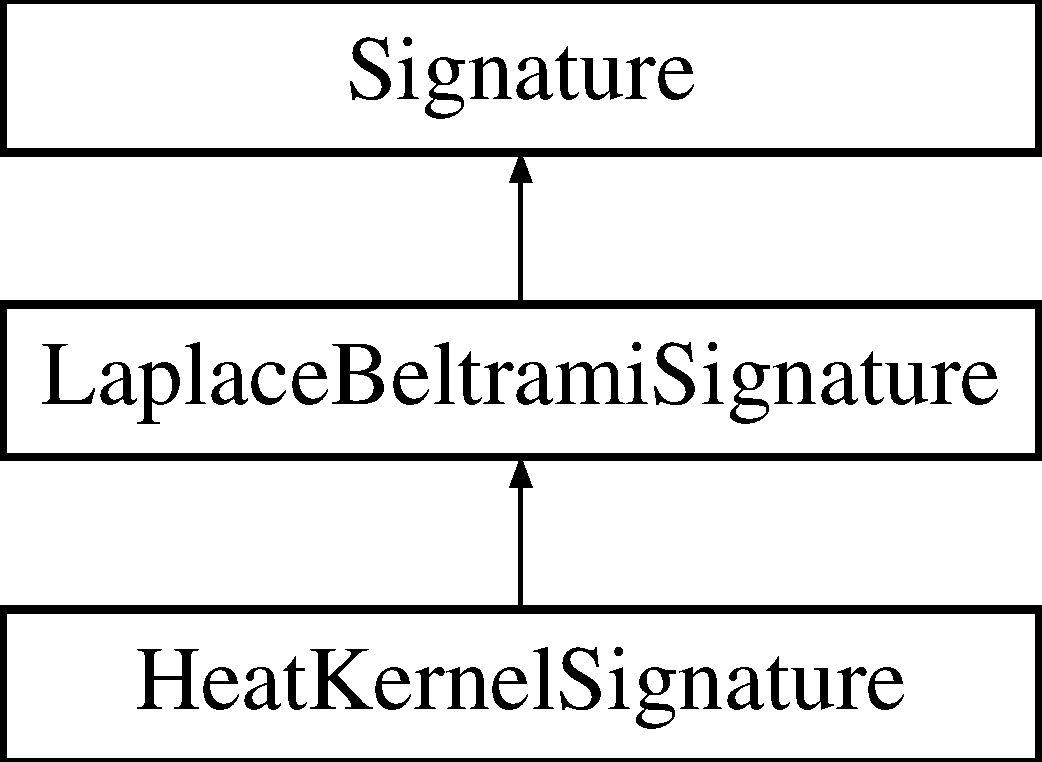
\includegraphics[height=3.000000cm]{class_heat_kernel_signature}
\end{center}
\end{figure}
\subsection*{Public Member Functions}
\begin{DoxyCompactItemize}
\item 
\hypertarget{class_heat_kernel_signature_ac21192a3ccebe61c2638991532495048}{}virtual void {\bfseries initialize} (\hyperlink{class_shape}{Shape} $\ast$shape, int dimension)\label{class_heat_kernel_signature_ac21192a3ccebe61c2638991532495048}

\end{DoxyCompactItemize}
\subsection*{Static Public Member Functions}
\begin{DoxyCompactItemize}
\item 
\hypertarget{class_heat_kernel_signature_a54d212433f1e77692b791c02576d25aa}{}static \hyperlink{class_laplace_beltrami_signature}{Laplace\+Beltrami\+Signature} $\ast$ {\bfseries create} ()\label{class_heat_kernel_signature_a54d212433f1e77692b791c02576d25aa}

\item 
\hypertarget{class_heat_kernel_signature_a3da9e323fe3c1af5d22e40d91a43c0a8}{}static string {\bfseries get\+Identifier} ()\label{class_heat_kernel_signature_a3da9e323fe3c1af5d22e40d91a43c0a8}

\end{DoxyCompactItemize}
\subsection*{Additional Inherited Members}


The documentation for this class was generated from the following files\+:\begin{DoxyCompactItemize}
\item 
src/domain/signatures/Heat\+Kernel\+Signature.\+h\item 
src/domain/signatures/Heat\+Kernel\+Signature.\+cpp\end{DoxyCompactItemize}

\hypertarget{classgeodesic_1_1_interval}{}\section{geodesic\+:\+:Interval Class Reference}
\label{classgeodesic_1_1_interval}\index{geodesic\+::\+Interval@{geodesic\+::\+Interval}}
Inheritance diagram for geodesic\+:\+:Interval\+:\begin{figure}[H]
\begin{center}
\leavevmode
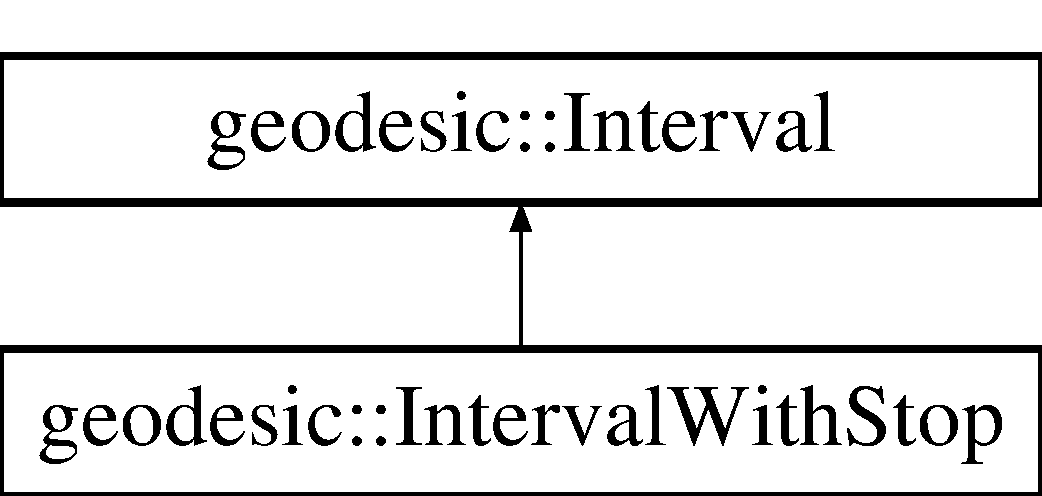
\includegraphics[height=2.000000cm]{classgeodesic_1_1_interval}
\end{center}
\end{figure}
\subsection*{Public Types}
\begin{DoxyCompactItemize}
\item 
\hypertarget{classgeodesic_1_1_interval_a60fb6352edb68be54a057468b02838d0}{}enum {\bfseries Direction\+Type} \{ {\bfseries F\+R\+O\+M\+\_\+\+F\+A\+C\+E\+\_\+0}, 
{\bfseries F\+R\+O\+M\+\_\+\+F\+A\+C\+E\+\_\+1}, 
{\bfseries F\+R\+O\+M\+\_\+\+S\+O\+U\+R\+C\+E}, 
{\bfseries U\+N\+D\+E\+F\+I\+N\+E\+D\+\_\+\+D\+I\+R\+E\+C\+T\+I\+O\+N}
 \}\label{classgeodesic_1_1_interval_a60fb6352edb68be54a057468b02838d0}

\end{DoxyCompactItemize}
\subsection*{Public Member Functions}
\begin{DoxyCompactItemize}
\item 
\hypertarget{classgeodesic_1_1_interval_a0882c603312c721d90882f25b4437b74}{}double {\bfseries signal} (double x)\label{classgeodesic_1_1_interval_a0882c603312c721d90882f25b4437b74}

\item 
\hypertarget{classgeodesic_1_1_interval_af259c70e3d8b4314f2b4b305ee0e6c7a}{}double {\bfseries max\+\_\+distance} (double end)\label{classgeodesic_1_1_interval_af259c70e3d8b4314f2b4b305ee0e6c7a}

\item 
\hypertarget{classgeodesic_1_1_interval_a3ead007bf10c60d7176384fb79108429}{}void {\bfseries compute\+\_\+min\+\_\+distance} (double stop)\label{classgeodesic_1_1_interval_a3ead007bf10c60d7176384fb79108429}

\item 
\hypertarget{classgeodesic_1_1_interval_a3674b70c9eb396e36b99ed743ad12276}{}bool {\bfseries operator()} (\hyperlink{classgeodesic_1_1_interval}{interval\+\_\+pointer} const x, \hyperlink{classgeodesic_1_1_interval}{interval\+\_\+pointer} const y) const \label{classgeodesic_1_1_interval_a3674b70c9eb396e36b99ed743ad12276}

\item 
\hypertarget{classgeodesic_1_1_interval_a617f1dbc519f7c56a9cb675f03fada92}{}double {\bfseries stop} ()\label{classgeodesic_1_1_interval_a617f1dbc519f7c56a9cb675f03fada92}

\item 
\hypertarget{classgeodesic_1_1_interval_a3fb3b9735b38db3fe64bc374afe5764a}{}double {\bfseries hypotenuse} (double a, double b)\label{classgeodesic_1_1_interval_a3fb3b9735b38db3fe64bc374afe5764a}

\item 
\hypertarget{classgeodesic_1_1_interval_acc19fb5bddb8f5ef4a0b3ae1c1868518}{}void {\bfseries find\+\_\+closest\+\_\+point} (double const x, double const y, double \&offset, double \&distance)\label{classgeodesic_1_1_interval_acc19fb5bddb8f5ef4a0b3ae1c1868518}

\item 
\hypertarget{classgeodesic_1_1_interval_a8e6b7a358505e45097482637dfcb91df}{}double \& {\bfseries start} ()\label{classgeodesic_1_1_interval_a8e6b7a358505e45097482637dfcb91df}

\item 
\hypertarget{classgeodesic_1_1_interval_ace2de9508089066782c6661b4dfdb220}{}double \& {\bfseries d} ()\label{classgeodesic_1_1_interval_ace2de9508089066782c6661b4dfdb220}

\item 
\hypertarget{classgeodesic_1_1_interval_ad97ef7bf3b77eb79719974ecb6a4b64c}{}double \& {\bfseries pseudo\+\_\+x} ()\label{classgeodesic_1_1_interval_ad97ef7bf3b77eb79719974ecb6a4b64c}

\item 
\hypertarget{classgeodesic_1_1_interval_a910c68345f1148d3f1c786ea122964be}{}double \& {\bfseries pseudo\+\_\+y} ()\label{classgeodesic_1_1_interval_a910c68345f1148d3f1c786ea122964be}

\item 
\hypertarget{classgeodesic_1_1_interval_a3805393c224c4cc767ed5a1fd4860744}{}double \& {\bfseries min} ()\label{classgeodesic_1_1_interval_a3805393c224c4cc767ed5a1fd4860744}

\item 
\hypertarget{classgeodesic_1_1_interval_a4c496edeb123149852a18a3e945e6ee8}{}\hyperlink{classgeodesic_1_1_interval}{interval\+\_\+pointer} \& {\bfseries next} ()\label{classgeodesic_1_1_interval_a4c496edeb123149852a18a3e945e6ee8}

\item 
\hypertarget{classgeodesic_1_1_interval_a74bad8b35168b14b2cfe72ca29411dce}{}\hyperlink{classgeodesic_1_1_edge}{edge\+\_\+pointer} \& {\bfseries edge} ()\label{classgeodesic_1_1_interval_a74bad8b35168b14b2cfe72ca29411dce}

\item 
\hypertarget{classgeodesic_1_1_interval_a116a7f1298cd2f08a10612f6cf8f353a}{}Direction\+Type \& {\bfseries direction} ()\label{classgeodesic_1_1_interval_a116a7f1298cd2f08a10612f6cf8f353a}

\item 
\hypertarget{classgeodesic_1_1_interval_a677eff57411bbcfd38fc32e3a0155f97}{}bool {\bfseries visible\+\_\+from\+\_\+source} ()\label{classgeodesic_1_1_interval_a677eff57411bbcfd38fc32e3a0155f97}

\item 
\hypertarget{classgeodesic_1_1_interval_a5e30261b5b844ed85e9e4ac4971a5355}{}unsigned \& {\bfseries source\+\_\+index} ()\label{classgeodesic_1_1_interval_a5e30261b5b844ed85e9e4ac4971a5355}

\item 
\hypertarget{classgeodesic_1_1_interval_a9e0e0bff3b09be45d7bc6f3dcfda3c36}{}void {\bfseries initialize} (\hyperlink{classgeodesic_1_1_edge}{edge\+\_\+pointer} edge, \hyperlink{classgeodesic_1_1_surface_point}{Surface\+Point} $\ast$point=N\+U\+L\+L, unsigned source\+\_\+index=0)\label{classgeodesic_1_1_interval_a9e0e0bff3b09be45d7bc6f3dcfda3c36}

\end{DoxyCompactItemize}
\subsection*{Protected Attributes}
\begin{DoxyCompactItemize}
\item 
\hypertarget{classgeodesic_1_1_interval_a8d89da9d69e8c74fc9f57a925e327e40}{}double {\bfseries m\+\_\+start}\label{classgeodesic_1_1_interval_a8d89da9d69e8c74fc9f57a925e327e40}

\item 
\hypertarget{classgeodesic_1_1_interval_adf67a2204c29d71b2e220714d4289dd2}{}double {\bfseries m\+\_\+d}\label{classgeodesic_1_1_interval_adf67a2204c29d71b2e220714d4289dd2}

\item 
\hypertarget{classgeodesic_1_1_interval_a92ad82dae3e03ba370f2a9dd95613df6}{}double {\bfseries m\+\_\+pseudo\+\_\+x}\label{classgeodesic_1_1_interval_a92ad82dae3e03ba370f2a9dd95613df6}

\item 
\hypertarget{classgeodesic_1_1_interval_ad470a1ccb1cbf146242a6d65d89836be}{}double {\bfseries m\+\_\+pseudo\+\_\+y}\label{classgeodesic_1_1_interval_ad470a1ccb1cbf146242a6d65d89836be}

\item 
\hypertarget{classgeodesic_1_1_interval_a9533fe7b0c0f5628cb285fbd9b5b471f}{}double {\bfseries m\+\_\+min}\label{classgeodesic_1_1_interval_a9533fe7b0c0f5628cb285fbd9b5b471f}

\item 
\hypertarget{classgeodesic_1_1_interval_a8baec5bb8eaf4564e11031bc2cc9e564}{}\hyperlink{classgeodesic_1_1_interval}{interval\+\_\+pointer} {\bfseries m\+\_\+next}\label{classgeodesic_1_1_interval_a8baec5bb8eaf4564e11031bc2cc9e564}

\item 
\hypertarget{classgeodesic_1_1_interval_a78f10c0e93ae78dc5678521343ef77bb}{}\hyperlink{classgeodesic_1_1_edge}{edge\+\_\+pointer} {\bfseries m\+\_\+edge}\label{classgeodesic_1_1_interval_a78f10c0e93ae78dc5678521343ef77bb}

\item 
\hypertarget{classgeodesic_1_1_interval_a64da19b53cef242f41bd8918eac779f5}{}unsigned {\bfseries m\+\_\+source\+\_\+index}\label{classgeodesic_1_1_interval_a64da19b53cef242f41bd8918eac779f5}

\item 
\hypertarget{classgeodesic_1_1_interval_a730c09218166ddcfc17759184c482ce8}{}Direction\+Type {\bfseries m\+\_\+direction}\label{classgeodesic_1_1_interval_a730c09218166ddcfc17759184c482ce8}

\end{DoxyCompactItemize}


The documentation for this class was generated from the following file\+:\begin{DoxyCompactItemize}
\item 
src/domain/metric/3rdparty/geodesic/geodesic\+\_\+algorithm\+\_\+exact\+\_\+elements.\+h\end{DoxyCompactItemize}

\hypertarget{classgeodesic_1_1_interval_list}{}\section{geodesic\+:\+:Interval\+List Class Reference}
\label{classgeodesic_1_1_interval_list}\index{geodesic\+::\+Interval\+List@{geodesic\+::\+Interval\+List}}
\subsection*{Public Member Functions}
\begin{DoxyCompactItemize}
\item 
\hypertarget{classgeodesic_1_1_interval_list_a006cc5985d16b3f007087e9f0e6f2be8}{}void {\bfseries clear} ()\label{classgeodesic_1_1_interval_list_a006cc5985d16b3f007087e9f0e6f2be8}

\item 
\hypertarget{classgeodesic_1_1_interval_list_a14de20c6cb848f62ff7dd48703c648f9}{}void {\bfseries initialize} (\hyperlink{classgeodesic_1_1_edge}{edge\+\_\+pointer} e)\label{classgeodesic_1_1_interval_list_a14de20c6cb848f62ff7dd48703c648f9}

\item 
\hypertarget{classgeodesic_1_1_interval_list_a3852850ab228257160ea1999a6ceeb6b}{}\hyperlink{classgeodesic_1_1_interval}{interval\+\_\+pointer} {\bfseries covering\+\_\+interval} (double offset)\label{classgeodesic_1_1_interval_list_a3852850ab228257160ea1999a6ceeb6b}

\item 
\hypertarget{classgeodesic_1_1_interval_list_a4d4da04f7be984dc4170a7904e0092cf}{}void {\bfseries find\+\_\+closest\+\_\+point} (\hyperlink{classgeodesic_1_1_surface_point}{Surface\+Point} $\ast$point, double \&offset, double \&distance, \hyperlink{classgeodesic_1_1_interval}{interval\+\_\+pointer} \&interval)\label{classgeodesic_1_1_interval_list_a4d4da04f7be984dc4170a7904e0092cf}

\item 
\hypertarget{classgeodesic_1_1_interval_list_a473a9e225447eb4ef46bf92e51f9fa71}{}unsigned {\bfseries number\+\_\+of\+\_\+intervals} ()\label{classgeodesic_1_1_interval_list_a473a9e225447eb4ef46bf92e51f9fa71}

\item 
\hypertarget{classgeodesic_1_1_interval_list_a132bd289ce2094f8799262b05867f618}{}\hyperlink{classgeodesic_1_1_interval}{interval\+\_\+pointer} {\bfseries last} ()\label{classgeodesic_1_1_interval_list_a132bd289ce2094f8799262b05867f618}

\item 
\hypertarget{classgeodesic_1_1_interval_list_ab182b06304c4a422daf9d66850046180}{}double {\bfseries signal} (double x)\label{classgeodesic_1_1_interval_list_ab182b06304c4a422daf9d66850046180}

\item 
\hypertarget{classgeodesic_1_1_interval_list_a39c74d06d5952ef1ea196c89820e81c3}{}\hyperlink{classgeodesic_1_1_interval}{interval\+\_\+pointer} \& {\bfseries first} ()\label{classgeodesic_1_1_interval_list_a39c74d06d5952ef1ea196c89820e81c3}

\item 
\hypertarget{classgeodesic_1_1_interval_list_af3d71b5e687ae7f3890e855be978426c}{}\hyperlink{classgeodesic_1_1_edge}{edge\+\_\+pointer} \& {\bfseries edge} ()\label{classgeodesic_1_1_interval_list_af3d71b5e687ae7f3890e855be978426c}

\end{DoxyCompactItemize}


The documentation for this class was generated from the following file\+:\begin{DoxyCompactItemize}
\item 
src/domain/metric/3rdparty/geodesic/geodesic\+\_\+algorithm\+\_\+exact\+\_\+elements.\+h\end{DoxyCompactItemize}

\hypertarget{structgeodesic_1_1_interval_with_stop}{}\section{geodesic\+:\+:Interval\+With\+Stop Struct Reference}
\label{structgeodesic_1_1_interval_with_stop}\index{geodesic\+::\+Interval\+With\+Stop@{geodesic\+::\+Interval\+With\+Stop}}
Inheritance diagram for geodesic\+:\+:Interval\+With\+Stop\+:\begin{figure}[H]
\begin{center}
\leavevmode
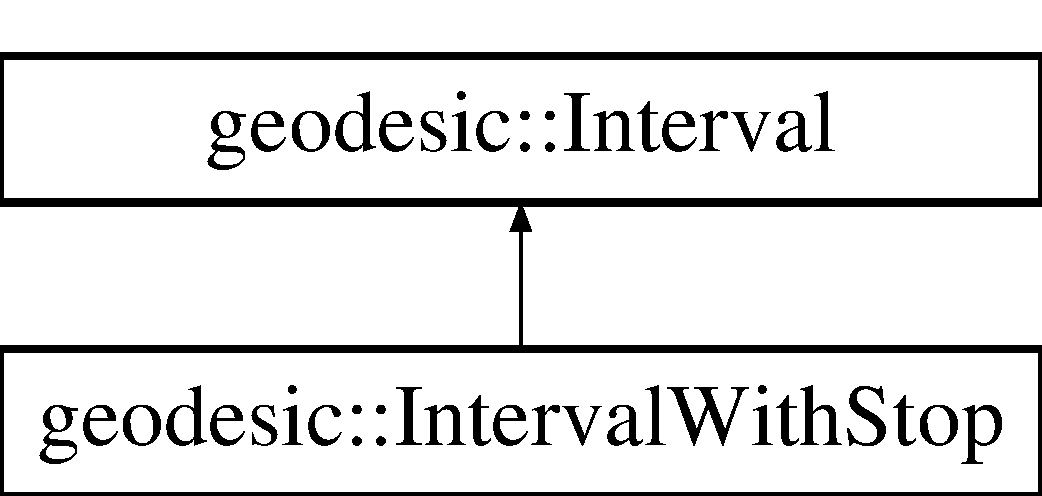
\includegraphics[height=2.000000cm]{structgeodesic_1_1_interval_with_stop}
\end{center}
\end{figure}
\subsection*{Public Member Functions}
\begin{DoxyCompactItemize}
\item 
\hypertarget{structgeodesic_1_1_interval_with_stop_ad40d1b39a99fe69dcf19aabbc17d1454}{}double \& {\bfseries stop} ()\label{structgeodesic_1_1_interval_with_stop_ad40d1b39a99fe69dcf19aabbc17d1454}

\end{DoxyCompactItemize}
\subsection*{Protected Attributes}
\begin{DoxyCompactItemize}
\item 
\hypertarget{structgeodesic_1_1_interval_with_stop_a5a646e636ac047b9b7d913eec283caf1}{}double {\bfseries m\+\_\+stop}\label{structgeodesic_1_1_interval_with_stop_a5a646e636ac047b9b7d913eec283caf1}

\end{DoxyCompactItemize}
\subsection*{Additional Inherited Members}


The documentation for this struct was generated from the following file\+:\begin{DoxyCompactItemize}
\item 
src/domain/metric/3rdparty/geodesic/geodesic\+\_\+algorithm\+\_\+exact\+\_\+elements.\+h\end{DoxyCompactItemize}

\hypertarget{class_laplace_beltrami_operator}{}\section{Laplace\+Beltrami\+Operator Class Reference}
\label{class_laplace_beltrami_operator}\index{Laplace\+Beltrami\+Operator@{Laplace\+Beltrami\+Operator}}
Inheritance diagram for Laplace\+Beltrami\+Operator\+:\begin{figure}[H]
\begin{center}
\leavevmode
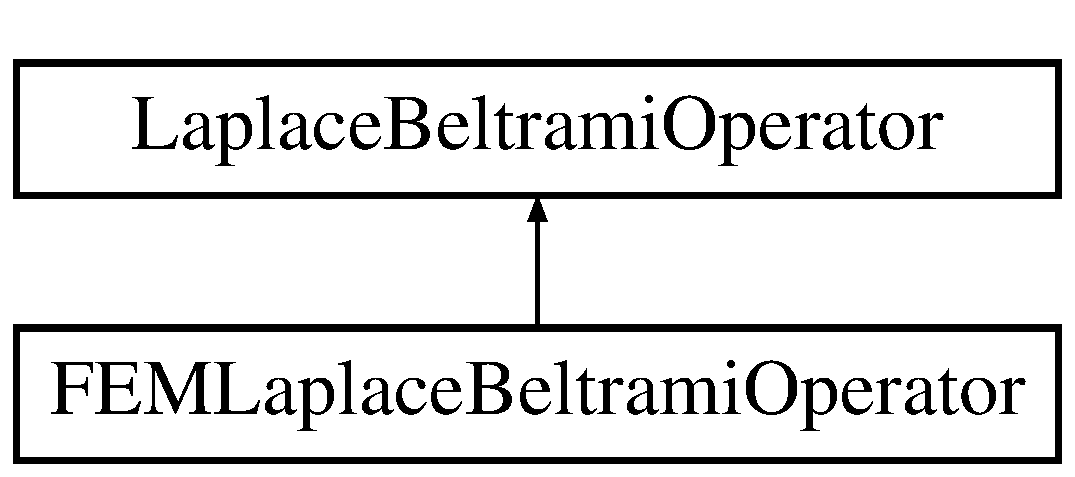
\includegraphics[height=2.000000cm]{class_laplace_beltrami_operator}
\end{center}
\end{figure}
\subsection*{Public Member Functions}
\begin{DoxyCompactItemize}
\item 
\hypertarget{class_laplace_beltrami_operator_a423822b9f1a6ac094b3f187e71936aa5}{}virtual void {\bfseries initialize} (\hyperlink{class_shape}{Shape} $\ast$shape, int number\+Of\+Eigenfunctions)\label{class_laplace_beltrami_operator_a423822b9f1a6ac094b3f187e71936aa5}

\item 
\hypertarget{class_laplace_beltrami_operator_a1f761e084fe593f6ef15ea4387939ccf}{}virtual void {\bfseries get\+Eigenfunction} (int i, \hyperlink{class_scalar_point_attribute}{Scalar\+Point\+Attribute} \&phi)=0\label{class_laplace_beltrami_operator_a1f761e084fe593f6ef15ea4387939ccf}

\item 
\hypertarget{class_laplace_beltrami_operator_a4574be5f06cdb575c3ae327140018df2}{}virtual double {\bfseries get\+Eigenvalue} (int i)=0\label{class_laplace_beltrami_operator_a4574be5f06cdb575c3ae327140018df2}

\item 
\hypertarget{class_laplace_beltrami_operator_aae4c110e717cc6324fec7bd32dd7fcc5}{}virtual void {\bfseries get\+Eigenfunction} (Petsc\+Int i, Vec $\ast$phi)=0\label{class_laplace_beltrami_operator_aae4c110e717cc6324fec7bd32dd7fcc5}

\item 
\hypertarget{class_laplace_beltrami_operator_a2b66fe8b96be6a53033886d8fc554732}{}virtual void {\bfseries get\+Eigenpair} (Petsc\+Int i, Vec $\ast$phi, Petsc\+Scalar $\ast$lambda)=0\label{class_laplace_beltrami_operator_a2b66fe8b96be6a53033886d8fc554732}

\item 
\hypertarget{class_laplace_beltrami_operator_a6edf61763fa043d3b1dcd0cf786ff04b}{}virtual void {\bfseries get\+Eigenfunction\+Matrix} (Mat $\ast$Phi)\label{class_laplace_beltrami_operator_a6edf61763fa043d3b1dcd0cf786ff04b}

\item 
\hypertarget{class_laplace_beltrami_operator_a49d8dda7af91604aa49641ac6c4d4e4e}{}virtual Mat $\ast$ {\bfseries get\+Mass\+Matrix} ()=0\label{class_laplace_beltrami_operator_a49d8dda7af91604aa49641ac6c4d4e4e}

\item 
\hypertarget{class_laplace_beltrami_operator_a338c9ffbc6343dfabbc76ac82da6e6b6}{}int {\bfseries get\+Number\+Of\+Eigenfunctions} ()\label{class_laplace_beltrami_operator_a338c9ffbc6343dfabbc76ac82da6e6b6}

\end{DoxyCompactItemize}
\subsection*{Protected Attributes}
\begin{DoxyCompactItemize}
\item 
\hypertarget{class_laplace_beltrami_operator_a76971e7079a1ff8b73e163406ac32ee7}{}\hyperlink{class_shape}{Shape} $\ast$ {\bfseries shape\+\_\+}\label{class_laplace_beltrami_operator_a76971e7079a1ff8b73e163406ac32ee7}

\item 
\hypertarget{class_laplace_beltrami_operator_a0e281e6ac8c0d72305f0c237e71b7d99}{}int {\bfseries number\+Of\+Eigenfunctions\+\_\+}\label{class_laplace_beltrami_operator_a0e281e6ac8c0d72305f0c237e71b7d99}

\end{DoxyCompactItemize}


The documentation for this class was generated from the following files\+:\begin{DoxyCompactItemize}
\item 
src/domain/Laplace\+Beltrami\+Operator.\+h\item 
src/domain/Laplace\+Beltrami\+Operator.\+cpp\end{DoxyCompactItemize}

\hypertarget{class_laplace_beltrami_signature}{}\section{Laplace\+Beltrami\+Signature Class Reference}
\label{class_laplace_beltrami_signature}\index{Laplace\+Beltrami\+Signature@{Laplace\+Beltrami\+Signature}}
Inheritance diagram for Laplace\+Beltrami\+Signature\+:\begin{figure}[H]
\begin{center}
\leavevmode
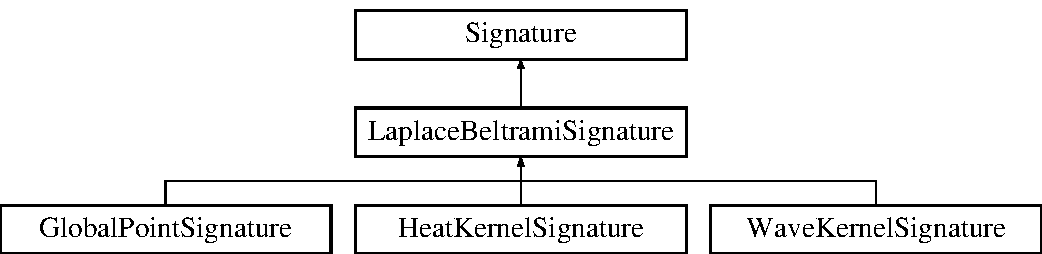
\includegraphics[height=3.000000cm]{class_laplace_beltrami_signature}
\end{center}
\end{figure}
\subsection*{Public Member Functions}
\begin{DoxyCompactItemize}
\item 
\hypertarget{class_laplace_beltrami_signature_ac0bf63ba94eba7581a9f45188f23b265}{}virtual void {\bfseries initialize} (\hyperlink{class_shape}{Shape} $\ast$shape, int dimension)\label{class_laplace_beltrami_signature_ac0bf63ba94eba7581a9f45188f23b265}

\item 
\hypertarget{class_laplace_beltrami_signature_a8155758d176dd0c137016302df1f6d7b}{}void {\bfseries set\+Laplacian} (\hyperlink{class_laplace_beltrami_operator}{Laplace\+Beltrami\+Operator} $\ast$laplacian)\label{class_laplace_beltrami_signature_a8155758d176dd0c137016302df1f6d7b}

\item 
\hypertarget{class_laplace_beltrami_signature_a6904095097912d71d9529d7b28aedd5f}{}void {\bfseries get\+Component} (int i, Vec $\ast$component)\label{class_laplace_beltrami_signature_a6904095097912d71d9529d7b28aedd5f}

\item 
\hypertarget{class_laplace_beltrami_signature_a1ec84385eba59549630b9c9742c6a04f}{}virtual void {\bfseries get\+Component} (int i, \hyperlink{class_scalar_point_attribute}{Scalar\+Point\+Attribute} \&component)\label{class_laplace_beltrami_signature_a1ec84385eba59549630b9c9742c6a04f}

\end{DoxyCompactItemize}
\subsection*{Protected Attributes}
\begin{DoxyCompactItemize}
\item 
\hypertarget{class_laplace_beltrami_signature_a5b0b11e9e61e889862246dd03a29d665}{}Mat {\bfseries signature\+\_\+}\label{class_laplace_beltrami_signature_a5b0b11e9e61e889862246dd03a29d665}

\item 
\hypertarget{class_laplace_beltrami_signature_af1fd997251e367f55f5fbaa7a75c8663}{}\hyperlink{class_laplace_beltrami_operator}{Laplace\+Beltrami\+Operator} $\ast$ {\bfseries laplacian\+\_\+}\label{class_laplace_beltrami_signature_af1fd997251e367f55f5fbaa7a75c8663}

\end{DoxyCompactItemize}


The documentation for this class was generated from the following files\+:\begin{DoxyCompactItemize}
\item 
src/domain/signatures/Laplace\+Beltrami\+Signature.\+h\item 
src/domain/signatures/Laplace\+Beltrami\+Signature.\+cpp\end{DoxyCompactItemize}

\hypertarget{classgeodesic_1_1_memory_allocator}{}\section{geodesic\+:\+:Memory\+Allocator$<$ T $>$ Class Template Reference}
\label{classgeodesic_1_1_memory_allocator}\index{geodesic\+::\+Memory\+Allocator$<$ T $>$@{geodesic\+::\+Memory\+Allocator$<$ T $>$}}
\subsection*{Public Types}
\begin{DoxyCompactItemize}
\item 
\hypertarget{classgeodesic_1_1_memory_allocator_a5bf49d03dcfd186a3e55d0766f6c7ac4}{}typedef T $\ast$ {\bfseries pointer}\label{classgeodesic_1_1_memory_allocator_a5bf49d03dcfd186a3e55d0766f6c7ac4}

\end{DoxyCompactItemize}
\subsection*{Public Member Functions}
\begin{DoxyCompactItemize}
\item 
\hypertarget{classgeodesic_1_1_memory_allocator_a991b8951be7af0e01bccf0d543fd9c69}{}{\bfseries Memory\+Allocator} (unsigned block\+\_\+size=1024, unsigned max\+\_\+number\+\_\+of\+\_\+blocks=1024)\label{classgeodesic_1_1_memory_allocator_a991b8951be7af0e01bccf0d543fd9c69}

\item 
\hypertarget{classgeodesic_1_1_memory_allocator_a169568619912780794522d946d58cd87}{}void {\bfseries clear} ()\label{classgeodesic_1_1_memory_allocator_a169568619912780794522d946d58cd87}

\item 
\hypertarget{classgeodesic_1_1_memory_allocator_a60563dcce45646630bba8b8a5533e087}{}void {\bfseries reset} (unsigned block\+\_\+size, unsigned max\+\_\+number\+\_\+of\+\_\+blocks)\label{classgeodesic_1_1_memory_allocator_a60563dcce45646630bba8b8a5533e087}

\item 
\hypertarget{classgeodesic_1_1_memory_allocator_aad7b63d11a97a054a8a7b45f29fdc391}{}pointer {\bfseries allocate} ()\label{classgeodesic_1_1_memory_allocator_aad7b63d11a97a054a8a7b45f29fdc391}

\item 
\hypertarget{classgeodesic_1_1_memory_allocator_a2ead9339bbb05eb76014b08bc1d5bfeb}{}void {\bfseries deallocate} (pointer p)\label{classgeodesic_1_1_memory_allocator_a2ead9339bbb05eb76014b08bc1d5bfeb}

\end{DoxyCompactItemize}


The documentation for this class was generated from the following file\+:\begin{DoxyCompactItemize}
\item 
src/domain/metric/3rdparty/geodesic/geodesic\+\_\+memory.\+h\end{DoxyCompactItemize}

\hypertarget{classgeodesic_1_1_mesh}{}\section{geodesic\+:\+:Mesh Class Reference}
\label{classgeodesic_1_1_mesh}\index{geodesic\+::\+Mesh@{geodesic\+::\+Mesh}}
\subsection*{Public Member Functions}
\begin{DoxyCompactItemize}
\item 
\hypertarget{classgeodesic_1_1_mesh_a93872801bd0c82c4586796a0d31023b1}{}{\footnotesize template$<$class Points , class Faces $>$ }\\void {\bfseries initialize\+\_\+mesh\+\_\+data} (unsigned num\+\_\+vertices, Points \&p, unsigned num\+\_\+faces, Faces \&tri)\label{classgeodesic_1_1_mesh_a93872801bd0c82c4586796a0d31023b1}

\item 
\hypertarget{classgeodesic_1_1_mesh_af3364382b9b1cd2762a12b644f4632b0}{}{\footnotesize template$<$class Points , class Faces $>$ }\\void {\bfseries initialize\+\_\+mesh\+\_\+data} (Points \&p, Faces \&tri)\label{classgeodesic_1_1_mesh_af3364382b9b1cd2762a12b644f4632b0}

\item 
\hypertarget{classgeodesic_1_1_mesh_a8b0c9bb6dec5f17d1d6798a5c4a91436}{}std\+::vector$<$ \hyperlink{classgeodesic_1_1_vertex}{Vertex} $>$ \& {\bfseries vertices} ()\label{classgeodesic_1_1_mesh_a8b0c9bb6dec5f17d1d6798a5c4a91436}

\item 
\hypertarget{classgeodesic_1_1_mesh_a4e972d008fb509a1fc1c8e12a050dde6}{}std\+::vector$<$ \hyperlink{classgeodesic_1_1_edge}{Edge} $>$ \& {\bfseries edges} ()\label{classgeodesic_1_1_mesh_a4e972d008fb509a1fc1c8e12a050dde6}

\item 
\hypertarget{classgeodesic_1_1_mesh_aea5069def2b66f0dfb008b16f11ce786}{}std\+::vector$<$ \hyperlink{classgeodesic_1_1_face}{Face} $>$ \& {\bfseries faces} ()\label{classgeodesic_1_1_mesh_aea5069def2b66f0dfb008b16f11ce786}

\item 
\hypertarget{classgeodesic_1_1_mesh_ad429dde54ea2a57b6e0bf245ba34b213}{}unsigned {\bfseries closest\+\_\+vertices} (\hyperlink{classgeodesic_1_1_surface_point}{Surface\+Point} $\ast$p, std\+::vector$<$ \hyperlink{classgeodesic_1_1_vertex}{vertex\+\_\+pointer} $>$ $\ast$storage=N\+U\+L\+L)\label{classgeodesic_1_1_mesh_ad429dde54ea2a57b6e0bf245ba34b213}

\end{DoxyCompactItemize}


The documentation for this class was generated from the following file\+:\begin{DoxyCompactItemize}
\item 
src/domain/metric/3rdparty/geodesic/geodesic\+\_\+mesh.\+h\end{DoxyCompactItemize}

\hypertarget{class_mesh_checker}{}\section{Mesh\+Checker Class Reference}
\label{class_mesh_checker}\index{Mesh\+Checker@{Mesh\+Checker}}
\subsection*{Public Member Functions}
\begin{DoxyCompactItemize}
\item 
\hypertarget{class_mesh_checker_a9952333587b195bfa117aa4003218043}{}{\bfseries Mesh\+Checker} (\hyperlink{class_shape}{Shape} $\ast$shape)\label{class_mesh_checker_a9952333587b195bfa117aa4003218043}

\item 
\hypertarget{class_mesh_checker_ae24c4e3f5feff68c83726fb23d97585f}{}bool {\bfseries check\+For\+Borders} (vector$<$ pair$<$ vtk\+Id\+Type, vtk\+Id\+Type $>$ $>$ $\ast$borders=nullptr)\label{class_mesh_checker_ae24c4e3f5feff68c83726fb23d97585f}

\item 
\hypertarget{class_mesh_checker_af43afc7f2b3882664f0ee2391c147efb}{}bool {\bfseries check\+Orientation} (vector$<$ pair$<$ vtk\+Id\+Type, vtk\+Id\+Type $>$ $>$ $\ast$unoriented=nullptr)\label{class_mesh_checker_af43afc7f2b3882664f0ee2391c147efb}

\item 
\hypertarget{class_mesh_checker_a98cde65ece5f709e4ef3657cb8129fa4}{}bool {\bfseries check\+Triangulation} (vector$<$ pair$<$ vtk\+Id\+Type, vtk\+Id\+Type $>$ $>$ $\ast$nontriangles=nullptr)\label{class_mesh_checker_a98cde65ece5f709e4ef3657cb8129fa4}

\item 
\hypertarget{class_mesh_checker_a95c42fdfb234e0be1d70ba255dbb5703}{}int {\bfseries check\+Number\+Of\+Regions} ()\label{class_mesh_checker_a95c42fdfb234e0be1d70ba255dbb5703}

\end{DoxyCompactItemize}


The documentation for this class was generated from the following files\+:\begin{DoxyCompactItemize}
\item 
src/domain/Mesh\+Checker.\+h\item 
src/domain/Mesh\+Checker.\+cpp\end{DoxyCompactItemize}

\hypertarget{class_ui_1_1_mesh_check_widget}{}\section{Ui\+:\+:Mesh\+Check\+Widget Class Reference}
\label{class_ui_1_1_mesh_check_widget}\index{Ui\+::\+Mesh\+Check\+Widget@{Ui\+::\+Mesh\+Check\+Widget}}
Inheritance diagram for Ui\+:\+:Mesh\+Check\+Widget\+:\begin{figure}[H]
\begin{center}
\leavevmode
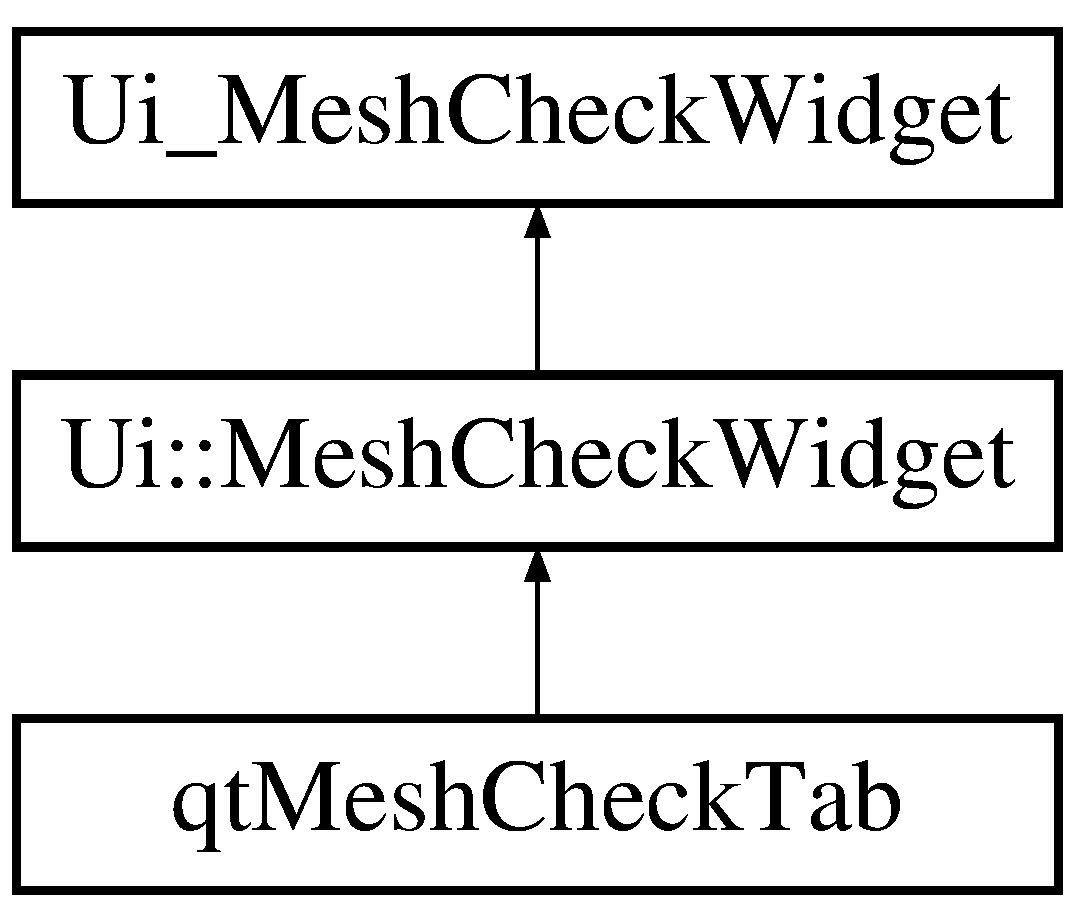
\includegraphics[height=3.000000cm]{class_ui_1_1_mesh_check_widget}
\end{center}
\end{figure}
\subsection*{Additional Inherited Members}


The documentation for this class was generated from the following file\+:\begin{DoxyCompactItemize}
\item 
build/ui\+\_\+meshcheck.\+h\end{DoxyCompactItemize}

\hypertarget{classgeodesic_1_1_mesh_element_base}{}\section{geodesic\+:\+:Mesh\+Element\+Base Class Reference}
\label{classgeodesic_1_1_mesh_element_base}\index{geodesic\+::\+Mesh\+Element\+Base@{geodesic\+::\+Mesh\+Element\+Base}}
Inheritance diagram for geodesic\+:\+:Mesh\+Element\+Base\+:\begin{figure}[H]
\begin{center}
\leavevmode
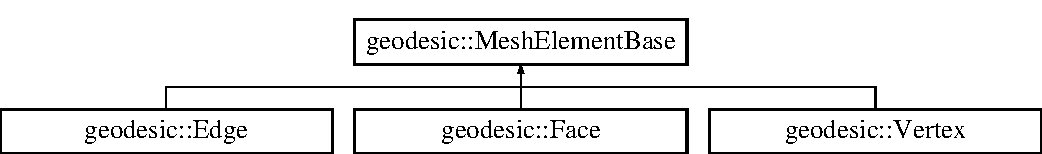
\includegraphics[height=2.000000cm]{classgeodesic_1_1_mesh_element_base}
\end{center}
\end{figure}
\subsection*{Public Types}
\begin{DoxyCompactItemize}
\item 
\hypertarget{classgeodesic_1_1_mesh_element_base_a8a106ee1a2039c65b2303b4cfc9bef86}{}typedef \hyperlink{classgeodesic_1_1_simple_vector}{Simple\+Vector}$<$ \hyperlink{classgeodesic_1_1_vertex}{vertex\+\_\+pointer} $>$ {\bfseries vertex\+\_\+pointer\+\_\+vector}\label{classgeodesic_1_1_mesh_element_base_a8a106ee1a2039c65b2303b4cfc9bef86}

\item 
\hypertarget{classgeodesic_1_1_mesh_element_base_a1b1600d4056b0dbddf6912c37306d200}{}typedef \hyperlink{classgeodesic_1_1_simple_vector}{Simple\+Vector}$<$ \hyperlink{classgeodesic_1_1_edge}{edge\+\_\+pointer} $>$ {\bfseries edge\+\_\+pointer\+\_\+vector}\label{classgeodesic_1_1_mesh_element_base_a1b1600d4056b0dbddf6912c37306d200}

\item 
\hypertarget{classgeodesic_1_1_mesh_element_base_a2d020d9d785ece39e2c1d930387fdd37}{}typedef \hyperlink{classgeodesic_1_1_simple_vector}{Simple\+Vector}$<$ \hyperlink{classgeodesic_1_1_face}{face\+\_\+pointer} $>$ {\bfseries face\+\_\+pointer\+\_\+vector}\label{classgeodesic_1_1_mesh_element_base_a2d020d9d785ece39e2c1d930387fdd37}

\end{DoxyCompactItemize}
\subsection*{Public Member Functions}
\begin{DoxyCompactItemize}
\item 
\hypertarget{classgeodesic_1_1_mesh_element_base_a480d07d33b01aed5525f428781aaa740}{}\hyperlink{classgeodesic_1_1_simple_vector}{vertex\+\_\+pointer\+\_\+vector} \& {\bfseries adjacent\+\_\+vertices} ()\label{classgeodesic_1_1_mesh_element_base_a480d07d33b01aed5525f428781aaa740}

\item 
\hypertarget{classgeodesic_1_1_mesh_element_base_a4f747e529f732bddf9439d10946c96d9}{}\hyperlink{classgeodesic_1_1_simple_vector}{edge\+\_\+pointer\+\_\+vector} \& {\bfseries adjacent\+\_\+edges} ()\label{classgeodesic_1_1_mesh_element_base_a4f747e529f732bddf9439d10946c96d9}

\item 
\hypertarget{classgeodesic_1_1_mesh_element_base_afe21848dd1b8009627c4818cd3f7a6b1}{}\hyperlink{classgeodesic_1_1_simple_vector}{face\+\_\+pointer\+\_\+vector} \& {\bfseries adjacent\+\_\+faces} ()\label{classgeodesic_1_1_mesh_element_base_afe21848dd1b8009627c4818cd3f7a6b1}

\item 
\hypertarget{classgeodesic_1_1_mesh_element_base_ad33adcf749c668a25fbd9d1f937222da}{}unsigned \& {\bfseries id} ()\label{classgeodesic_1_1_mesh_element_base_ad33adcf749c668a25fbd9d1f937222da}

\item 
\hypertarget{classgeodesic_1_1_mesh_element_base_a667dabb1394e5611a5486da711b1962b}{}Point\+Type {\bfseries type} ()\label{classgeodesic_1_1_mesh_element_base_a667dabb1394e5611a5486da711b1962b}

\end{DoxyCompactItemize}
\subsection*{Protected Attributes}
\begin{DoxyCompactItemize}
\item 
\hypertarget{classgeodesic_1_1_mesh_element_base_af60cffe50087e9b5ea770e7ab8bcaddb}{}\hyperlink{classgeodesic_1_1_simple_vector}{vertex\+\_\+pointer\+\_\+vector} {\bfseries m\+\_\+adjacent\+\_\+vertices}\label{classgeodesic_1_1_mesh_element_base_af60cffe50087e9b5ea770e7ab8bcaddb}

\item 
\hypertarget{classgeodesic_1_1_mesh_element_base_a113429a05d2e89b39ee70b011764ff47}{}\hyperlink{classgeodesic_1_1_simple_vector}{edge\+\_\+pointer\+\_\+vector} {\bfseries m\+\_\+adjacent\+\_\+edges}\label{classgeodesic_1_1_mesh_element_base_a113429a05d2e89b39ee70b011764ff47}

\item 
\hypertarget{classgeodesic_1_1_mesh_element_base_a455d7b86e0a9affa2301ee21b77c52bc}{}\hyperlink{classgeodesic_1_1_simple_vector}{face\+\_\+pointer\+\_\+vector} {\bfseries m\+\_\+adjacent\+\_\+faces}\label{classgeodesic_1_1_mesh_element_base_a455d7b86e0a9affa2301ee21b77c52bc}

\item 
\hypertarget{classgeodesic_1_1_mesh_element_base_a6173e3b72644fc0e736bb2ec74b6034d}{}unsigned {\bfseries m\+\_\+id}\label{classgeodesic_1_1_mesh_element_base_a6173e3b72644fc0e736bb2ec74b6034d}

\item 
\hypertarget{classgeodesic_1_1_mesh_element_base_aaf22414cde7d8103747cd12e2f031bd1}{}Point\+Type {\bfseries m\+\_\+type}\label{classgeodesic_1_1_mesh_element_base_aaf22414cde7d8103747cd12e2f031bd1}

\end{DoxyCompactItemize}


The documentation for this class was generated from the following file\+:\begin{DoxyCompactItemize}
\item 
src/domain/metric/3rdparty/geodesic/geodesic\+\_\+mesh\+\_\+elements.\+h\end{DoxyCompactItemize}

\hypertarget{class_metric}{}\section{Metric Class Reference}
\label{class_metric}\index{Metric@{Metric}}
Inheritance diagram for Metric\+:\begin{figure}[H]
\begin{center}
\leavevmode
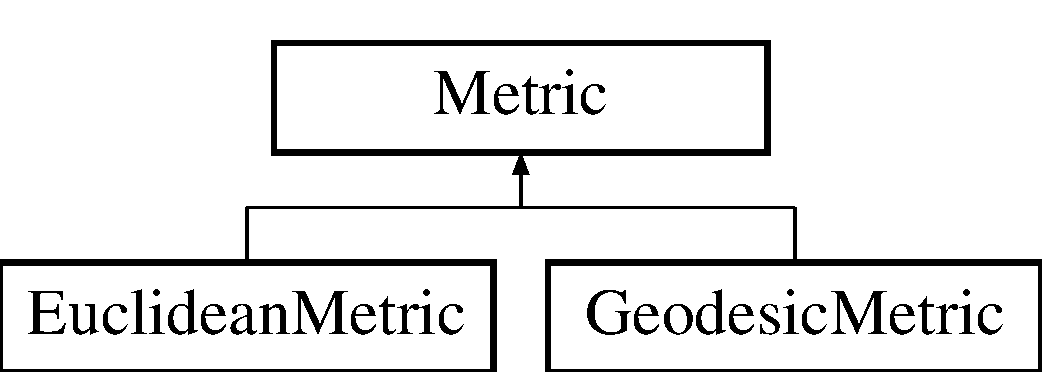
\includegraphics[height=2.000000cm]{class_metric}
\end{center}
\end{figure}
\subsection*{Public Member Functions}
\begin{DoxyCompactItemize}
\item 
\hypertarget{class_metric_afa7ed1a7ecc5039c24f7dab39ecaaaf0}{}virtual void {\bfseries initialize} (\hyperlink{class_shape}{Shape} $\ast$shape)\label{class_metric_afa7ed1a7ecc5039c24f7dab39ecaaaf0}

\item 
\hypertarget{class_metric_a51b89ee4ecb69e423cb8af22582ba09c}{}virtual double {\bfseries get\+Distance} (vtk\+Id\+Type a, vtk\+Id\+Type b)=0\label{class_metric_a51b89ee4ecb69e423cb8af22582ba09c}

\item 
\hypertarget{class_metric_ae2a68e0d2a63063909b92628939df012}{}virtual void {\bfseries get\+All\+Distances} (\hyperlink{class_scalar_point_attribute}{Scalar\+Point\+Attribute} \&distances, vtk\+Id\+Type source)=0\label{class_metric_ae2a68e0d2a63063909b92628939df012}

\item 
\hypertarget{class_metric_a2f4c68531fa9470847308cfdc9c11367}{}virtual vtk\+Id\+Type {\bfseries get\+Farthest\+Point} (vtk\+Smart\+Pointer$<$ vtk\+Id\+List $>$ sources)=0\label{class_metric_a2f4c68531fa9470847308cfdc9c11367}

\item 
\hypertarget{class_metric_aee48cf03e0d8c3f08c9bf9993fe3de87}{}virtual vtk\+Smart\+Pointer$<$ vtk\+Id\+List $>$ {\bfseries get\+Voronoi\+Cells} (vtk\+Smart\+Pointer$<$ vtk\+Id\+List $>$ seeds)=0\label{class_metric_aee48cf03e0d8c3f08c9bf9993fe3de87}

\item 
\hypertarget{class_metric_aab7d021672694fbec4c0742f9f33bbe0}{}\hyperlink{class_shape}{Shape} $\ast$ {\bfseries get\+Shape} ()\label{class_metric_aab7d021672694fbec4c0742f9f33bbe0}

\end{DoxyCompactItemize}
\subsection*{Protected Attributes}
\begin{DoxyCompactItemize}
\item 
\hypertarget{class_metric_adce68fb48ab77652ccab3dc7b017ea7c}{}\hyperlink{class_shape}{Shape} $\ast$ {\bfseries shape\+\_\+}\label{class_metric_adce68fb48ab77652ccab3dc7b017ea7c}

\end{DoxyCompactItemize}


The documentation for this class was generated from the following file\+:\begin{DoxyCompactItemize}
\item 
src/domain/metric/Metric.\+h\end{DoxyCompactItemize}

\hypertarget{class_metric_sampling}{}\section{Metric\+Sampling Class Reference}
\label{class_metric_sampling}\index{Metric\+Sampling@{Metric\+Sampling}}
Inheritance diagram for Metric\+Sampling\+:\begin{figure}[H]
\begin{center}
\leavevmode
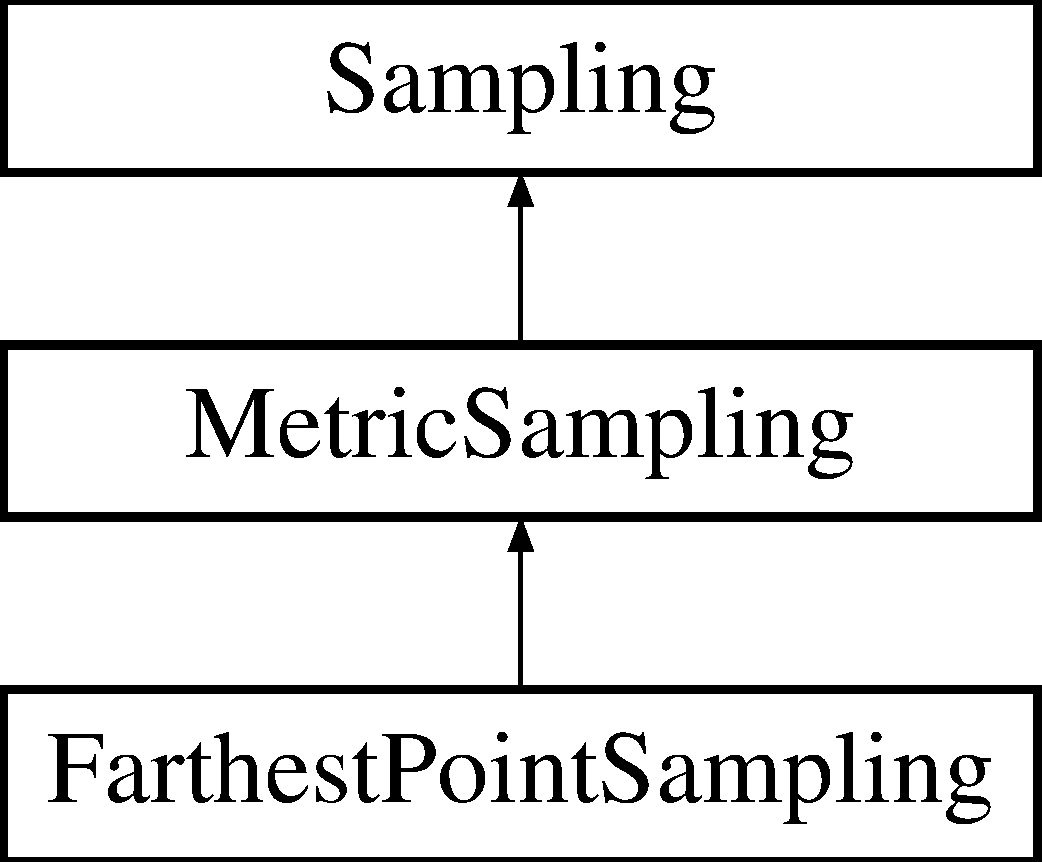
\includegraphics[height=3.000000cm]{class_metric_sampling}
\end{center}
\end{figure}
\subsection*{Public Member Functions}
\begin{DoxyCompactItemize}
\item 
\hypertarget{class_metric_sampling_aff86fe5597a6d0f49f07595cd2770296}{}void {\bfseries set\+Metric} (\hyperlink{class_metric}{Metric} $\ast$metric)\label{class_metric_sampling_aff86fe5597a6d0f49f07595cd2770296}

\end{DoxyCompactItemize}
\subsection*{Protected Attributes}
\begin{DoxyCompactItemize}
\item 
\hypertarget{class_metric_sampling_a5374fd52d959aece73b748e4d45ca328}{}\hyperlink{class_metric}{Metric} $\ast$ {\bfseries metric\+\_\+}\label{class_metric_sampling_a5374fd52d959aece73b748e4d45ca328}

\end{DoxyCompactItemize}


The documentation for this class was generated from the following files\+:\begin{DoxyCompactItemize}
\item 
src/domain/samplings/Metric\+Sampling.\+h\item 
src/domain/samplings/Metric\+Sampling.\+cpp\end{DoxyCompactItemize}

\hypertarget{classgeodesic_1_1_output_buffer}{}\section{geodesic\+:\+:Output\+Buffer Class Reference}
\label{classgeodesic_1_1_output_buffer}\index{geodesic\+::\+Output\+Buffer@{geodesic\+::\+Output\+Buffer}}
\subsection*{Public Member Functions}
\begin{DoxyCompactItemize}
\item 
\hypertarget{classgeodesic_1_1_output_buffer_ad3e44f392d1a9a26f9474b7508d39b58}{}void {\bfseries clear} ()\label{classgeodesic_1_1_output_buffer_ad3e44f392d1a9a26f9474b7508d39b58}

\item 
\hypertarget{classgeodesic_1_1_output_buffer_a789926b2e2c44942107610455ff62341}{}{\footnotesize template$<$class T $>$ }\\T $\ast$ {\bfseries allocate} (unsigned n)\label{classgeodesic_1_1_output_buffer_a789926b2e2c44942107610455ff62341}

\item 
\hypertarget{classgeodesic_1_1_output_buffer_ad895277754ee3eaf927f48794100fbc4}{}{\footnotesize template$<$class T $>$ }\\T $\ast$ {\bfseries get} ()\label{classgeodesic_1_1_output_buffer_ad895277754ee3eaf927f48794100fbc4}

\item 
\hypertarget{classgeodesic_1_1_output_buffer_aa8e58bceab56ff5da47485aef7686730}{}{\footnotesize template$<$class T $>$ }\\unsigned {\bfseries capacity} ()\label{classgeodesic_1_1_output_buffer_aa8e58bceab56ff5da47485aef7686730}

\end{DoxyCompactItemize}


The documentation for this class was generated from the following file\+:\begin{DoxyCompactItemize}
\item 
src/domain/metric/3rdparty/geodesic/geodesic\+\_\+memory.\+h\end{DoxyCompactItemize}

\hypertarget{class_petsc_helper}{}\section{Petsc\+Helper Class Reference}
\label{class_petsc_helper}\index{Petsc\+Helper@{Petsc\+Helper}}
\subsection*{Static Public Member Functions}
\begin{DoxyCompactItemize}
\item 
\hypertarget{class_petsc_helper_a322ae6e79127333879141c4a30d339dc}{}static void {\bfseries set\+Block} (Mat \&A, Mat \&B, Petsc\+Int i, Petsc\+Int j)\label{class_petsc_helper_a322ae6e79127333879141c4a30d339dc}

\item 
\hypertarget{class_petsc_helper_af7852884a00a9819e928e16553898b47}{}static void {\bfseries set\+Row} (Mat \&A, Vec \&ai, Petsc\+Int i)\label{class_petsc_helper_af7852884a00a9819e928e16553898b47}

\item 
\hypertarget{class_petsc_helper_a8d80ba637aaeac16f8bfd2af40f3983d}{}static void {\bfseries get\+Row} (Vec \&ai, Mat \&A, Petsc\+Int i)\label{class_petsc_helper_a8d80ba637aaeac16f8bfd2af40f3983d}

\item 
\hypertarget{class_petsc_helper_a6be1aa6939210adc087cff94ef217267}{}static void {\bfseries set\+Column} (Mat \&A, Vec \&ai, Petsc\+Int i)\label{class_petsc_helper_a6be1aa6939210adc087cff94ef217267}

\item 
\hypertarget{class_petsc_helper_a30c7c416ad5fdd5d4d9edb1ea4a3936f}{}static void {\bfseries reshape} (Mat \&B, Vec \&b, Petsc\+Int m, Petsc\+Int n)\label{class_petsc_helper_a30c7c416ad5fdd5d4d9edb1ea4a3936f}

\end{DoxyCompactItemize}


The documentation for this class was generated from the following files\+:\begin{DoxyCompactItemize}
\item 
src/domain/Petsc\+Helper.\+h\item 
src/domain/Petsc\+Helper.\+cpp\end{DoxyCompactItemize}

\hypertarget{classgeodesic_1_1_point3_d}{}\section{geodesic\+:\+:Point3\+D Class Reference}
\label{classgeodesic_1_1_point3_d}\index{geodesic\+::\+Point3\+D@{geodesic\+::\+Point3\+D}}
Inheritance diagram for geodesic\+:\+:Point3\+D\+:\begin{figure}[H]
\begin{center}
\leavevmode
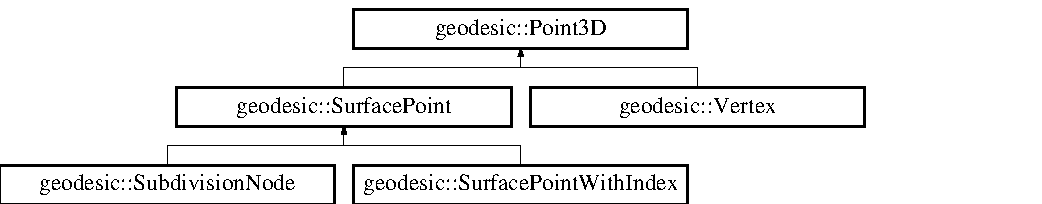
\includegraphics[height=2.745098cm]{classgeodesic_1_1_point3_d}
\end{center}
\end{figure}
\subsection*{Public Member Functions}
\begin{DoxyCompactItemize}
\item 
\hypertarget{classgeodesic_1_1_point3_d_af51b212e1c7783a152d051bfba01477d}{}{\bfseries Point3\+D} (\hyperlink{classgeodesic_1_1_point3_d}{Point3\+D} $\ast$p)\label{classgeodesic_1_1_point3_d_af51b212e1c7783a152d051bfba01477d}

\item 
\hypertarget{classgeodesic_1_1_point3_d_a6d17f1e0e0fec59ef52bdf57b15dcd45}{}double $\ast$ {\bfseries xyz} ()\label{classgeodesic_1_1_point3_d_a6d17f1e0e0fec59ef52bdf57b15dcd45}

\item 
\hypertarget{classgeodesic_1_1_point3_d_a1dcd0a527168c55641f24cd6f28dedd1}{}double \& {\bfseries x} ()\label{classgeodesic_1_1_point3_d_a1dcd0a527168c55641f24cd6f28dedd1}

\item 
\hypertarget{classgeodesic_1_1_point3_d_abd341931f55593d0fe5eb53b554ec000}{}double \& {\bfseries y} ()\label{classgeodesic_1_1_point3_d_abd341931f55593d0fe5eb53b554ec000}

\item 
\hypertarget{classgeodesic_1_1_point3_d_a98c3395b7346aecf1410076e0cfc00f3}{}double \& {\bfseries z} ()\label{classgeodesic_1_1_point3_d_a98c3395b7346aecf1410076e0cfc00f3}

\item 
\hypertarget{classgeodesic_1_1_point3_d_a09432372bbf3c0b1b3c867b30079eb9f}{}void {\bfseries set} (double new\+\_\+x, double new\+\_\+y, double new\+\_\+z)\label{classgeodesic_1_1_point3_d_a09432372bbf3c0b1b3c867b30079eb9f}

\item 
\hypertarget{classgeodesic_1_1_point3_d_a44c9221725a8d3ecd173639a61f846c4}{}void {\bfseries set} (double $\ast$data)\label{classgeodesic_1_1_point3_d_a44c9221725a8d3ecd173639a61f846c4}

\item 
\hypertarget{classgeodesic_1_1_point3_d_a1e9add700f5632bb84ca819f2f7dba9c}{}double {\bfseries distance} (double $\ast$v)\label{classgeodesic_1_1_point3_d_a1e9add700f5632bb84ca819f2f7dba9c}

\item 
\hypertarget{classgeodesic_1_1_point3_d_a818ba92398944178025b125b95761702}{}double {\bfseries distance} (\hyperlink{classgeodesic_1_1_point3_d}{Point3\+D} $\ast$v)\label{classgeodesic_1_1_point3_d_a818ba92398944178025b125b95761702}

\item 
\hypertarget{classgeodesic_1_1_point3_d_a97f5b5c5e1d9c54dfe9e838ba1988dc3}{}void {\bfseries add} (\hyperlink{classgeodesic_1_1_point3_d}{Point3\+D} $\ast$v)\label{classgeodesic_1_1_point3_d_a97f5b5c5e1d9c54dfe9e838ba1988dc3}

\item 
\hypertarget{classgeodesic_1_1_point3_d_ac50ecd9e0432f4b4daee76694d850626}{}void {\bfseries multiply} (double v)\label{classgeodesic_1_1_point3_d_ac50ecd9e0432f4b4daee76694d850626}

\end{DoxyCompactItemize}


The documentation for this class was generated from the following file\+:\begin{DoxyCompactItemize}
\item 
src/domain/metric/3rdparty/geodesic/geodesic\+\_\+mesh\+\_\+elements.\+h\end{DoxyCompactItemize}

\hypertarget{class_point_correspondence}{}\section{Point\+Correspondence Class Reference}
\label{class_point_correspondence}\index{Point\+Correspondence@{Point\+Correspondence}}
Inheritance diagram for Point\+Correspondence\+:\begin{figure}[H]
\begin{center}
\leavevmode
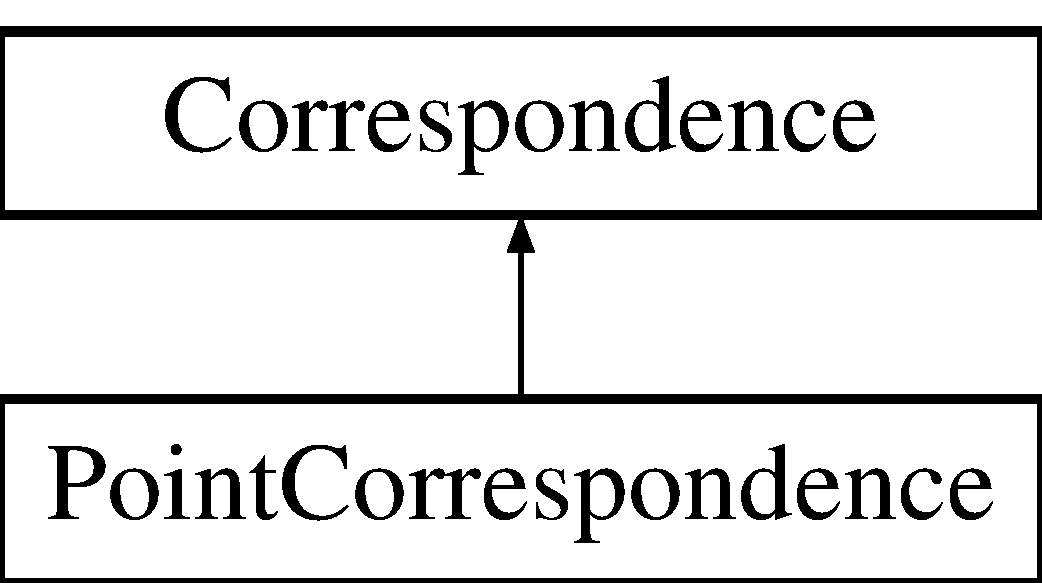
\includegraphics[height=2.000000cm]{class_point_correspondence}
\end{center}
\end{figure}
\subsection*{Public Member Functions}
\begin{DoxyCompactItemize}
\item 
\hypertarget{class_point_correspondence_a4ae058435459065fad930bf6f5eeb355}{}{\bfseries Point\+Correspondence} (vtk\+Smart\+Pointer$<$ vtk\+Renderer $>$ renderer, \hyperlink{class_point_correspondence_data}{Point\+Correspondence\+Data} $\ast$data)\label{class_point_correspondence_a4ae058435459065fad930bf6f5eeb355}

\item 
\hypertarget{class_point_correspondence_a194d358a1a9cc838690359cbd5902a4b}{}{\bfseries Point\+Correspondence} (vtk\+Smart\+Pointer$<$ vtk\+Renderer $>$ renderer, \hyperlink{class_point_correspondence_data}{Point\+Correspondence\+Data} $\ast$data, \hyperlink{class_hash_map}{Hash\+Map}$<$ vtk\+Actor $\ast$, \hyperlink{class_shape}{Shape} $\ast$ $>$ \&shapes)\label{class_point_correspondence_a194d358a1a9cc838690359cbd5902a4b}

\item 
\hypertarget{class_point_correspondence_a2dc1d4de5d4bf8f9f10d909275eb4935}{}\hyperlink{class_point_correspondence_data}{Point\+Correspondence\+Data} $\ast$ {\bfseries get\+Data} ()\label{class_point_correspondence_a2dc1d4de5d4bf8f9f10d909275eb4935}

\end{DoxyCompactItemize}
\subsection*{Protected Member Functions}
\begin{DoxyCompactItemize}
\item 
\hypertarget{class_point_correspondence_a474f835c1093311ae7c240b6db096531}{}virtual void {\bfseries initialize\+Actor} (vtk\+Smart\+Pointer$<$ vtk\+Actor $>$ actor, \hyperlink{class_shape}{Shape} $\ast$shape, vtk\+Id\+Type point\+Id)\label{class_point_correspondence_a474f835c1093311ae7c240b6db096531}

\item 
\hypertarget{class_point_correspondence_abafeb29cdc31f70e1848a78ffe410f26}{}virtual void {\bfseries get\+Correspondence\+Point} (double point\mbox{[}3\mbox{]}, \hyperlink{class_shape}{Shape} $\ast$shape, vtk\+Id\+Type)\label{class_point_correspondence_abafeb29cdc31f70e1848a78ffe410f26}

\end{DoxyCompactItemize}
\subsection*{Additional Inherited Members}


The documentation for this class was generated from the following files\+:\begin{DoxyCompactItemize}
\item 
src/domain/correspondences/Point\+Correspondence.\+h\item 
src/domain/correspondences/Point\+Correspondence.\+cpp\end{DoxyCompactItemize}

\hypertarget{class_point_correspondence_data}{}\section{Point\+Correspondence\+Data Class Reference}
\label{class_point_correspondence_data}\index{Point\+Correspondence\+Data@{Point\+Correspondence\+Data}}
Inheritance diagram for Point\+Correspondence\+Data\+:\begin{figure}[H]
\begin{center}
\leavevmode
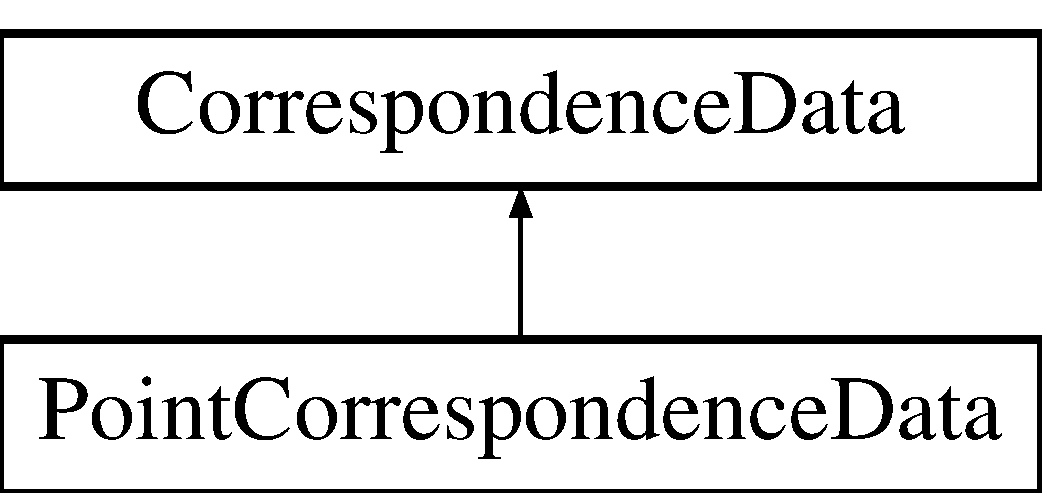
\includegraphics[height=2.000000cm]{class_point_correspondence_data}
\end{center}
\end{figure}
\subsection*{Public Member Functions}
\begin{DoxyCompactItemize}
\item 
\hypertarget{class_point_correspondence_data_adc639a5dff9489880a880bb990befd0e}{}{\bfseries Point\+Correspondence\+Data} (vtk\+Id\+Type id)\label{class_point_correspondence_data_adc639a5dff9489880a880bb990befd0e}

\item 
\hypertarget{class_point_correspondence_data_afe00b9700744499a366075346025e41a}{}virtual string {\bfseries get\+Type} ()\label{class_point_correspondence_data_afe00b9700744499a366075346025e41a}

\end{DoxyCompactItemize}
\subsection*{Additional Inherited Members}


The documentation for this class was generated from the following file\+:\begin{DoxyCompactItemize}
\item 
src/domain/correspondences/Point\+Correspondence\+Data.\+h\end{DoxyCompactItemize}

\hypertarget{class_point_correspondence_picker}{}\section{Point\+Correspondence\+Picker Class Reference}
\label{class_point_correspondence_picker}\index{Point\+Correspondence\+Picker@{Point\+Correspondence\+Picker}}
Inheritance diagram for Point\+Correspondence\+Picker\+:\begin{figure}[H]
\begin{center}
\leavevmode
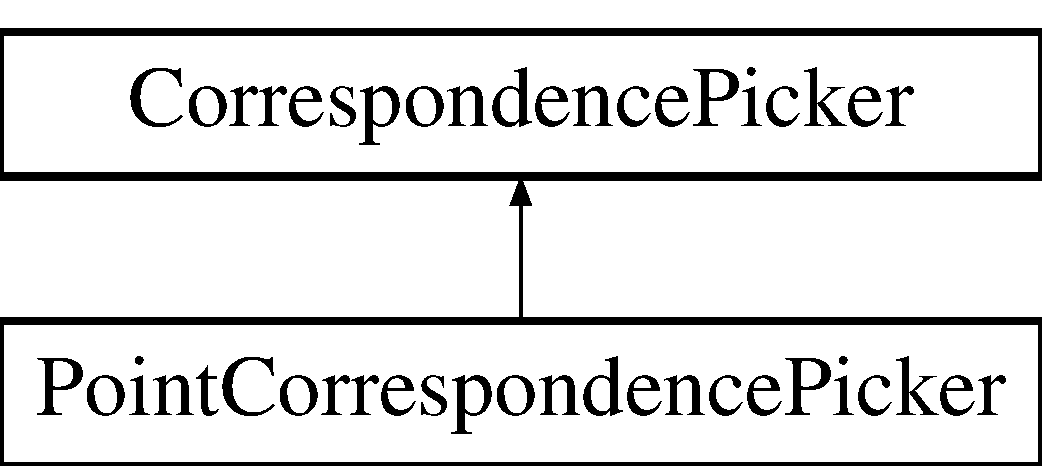
\includegraphics[height=2.000000cm]{class_point_correspondence_picker}
\end{center}
\end{figure}
\subsection*{Public Member Functions}
\begin{DoxyCompactItemize}
\item 
\hypertarget{class_point_correspondence_picker_a07a5158a5629e78afadc955674109a61}{}{\bfseries Point\+Correspondence\+Picker} (vtk\+Renderer $\ast$renderer, int \&last\+Insert\+Correspondence\+I\+D)\label{class_point_correspondence_picker_a07a5158a5629e78afadc955674109a61}

\end{DoxyCompactItemize}
\subsection*{Additional Inherited Members}


The documentation for this class was generated from the following files\+:\begin{DoxyCompactItemize}
\item 
src/view/Point\+Correspondence\+Picker.\+h\item 
src/view/Point\+Correspondence\+Picker.\+cpp\end{DoxyCompactItemize}

\hypertarget{class_ui_1_1_point_correspondences_widget}{}\section{Ui\+:\+:Point\+Correspondences\+Widget Class Reference}
\label{class_ui_1_1_point_correspondences_widget}\index{Ui\+::\+Point\+Correspondences\+Widget@{Ui\+::\+Point\+Correspondences\+Widget}}
Inheritance diagram for Ui\+:\+:Point\+Correspondences\+Widget\+:\begin{figure}[H]
\begin{center}
\leavevmode
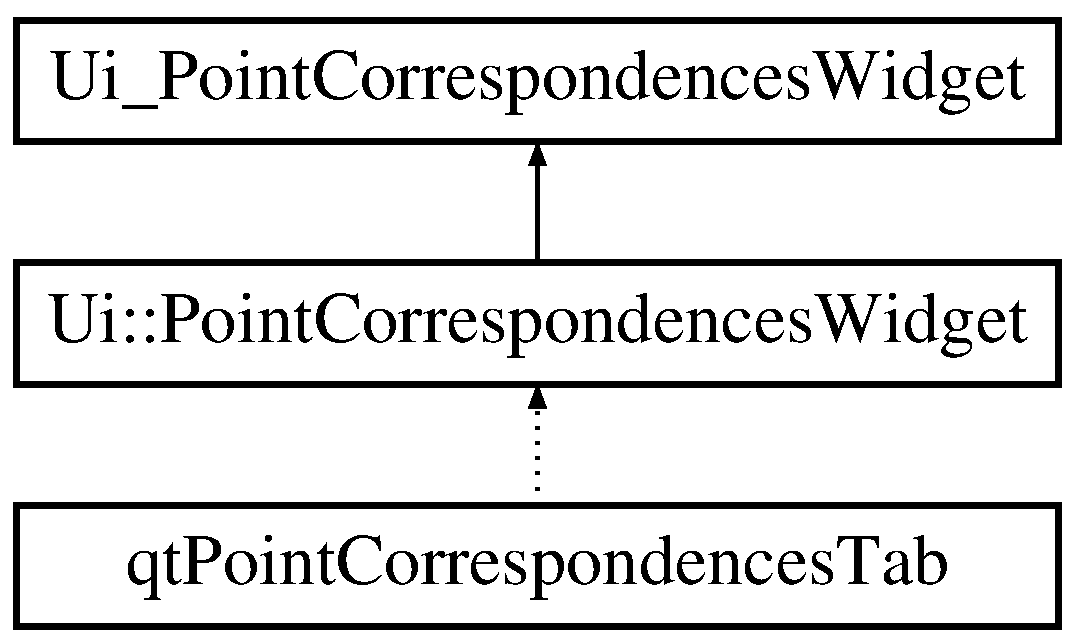
\includegraphics[height=3.000000cm]{class_ui_1_1_point_correspondences_widget}
\end{center}
\end{figure}
\subsection*{Additional Inherited Members}


The documentation for this class was generated from the following file\+:\begin{DoxyCompactItemize}
\item 
build/ui\+\_\+point\+Correspondences.\+h\end{DoxyCompactItemize}

\hypertarget{structqt__meta__stringdata__qt_correspondence_coloring_tab__t}{}\section{qt\+\_\+meta\+\_\+stringdata\+\_\+qt\+Correspondence\+Coloring\+Tab\+\_\+t Struct Reference}
\label{structqt__meta__stringdata__qt_correspondence_coloring_tab__t}\index{qt\+\_\+meta\+\_\+stringdata\+\_\+qt\+Correspondence\+Coloring\+Tab\+\_\+t@{qt\+\_\+meta\+\_\+stringdata\+\_\+qt\+Correspondence\+Coloring\+Tab\+\_\+t}}
\subsection*{Public Attributes}
\begin{DoxyCompactItemize}
\item 
\hypertarget{structqt__meta__stringdata__qt_correspondence_coloring_tab__t_a8f9997a78891e426bf74cf662e218140}{}Q\+Byte\+Array\+Data {\bfseries data} \mbox{[}3\mbox{]}\label{structqt__meta__stringdata__qt_correspondence_coloring_tab__t_a8f9997a78891e426bf74cf662e218140}

\item 
\hypertarget{structqt__meta__stringdata__qt_correspondence_coloring_tab__t_a1fbb8434b528f989c3189ab3bfaa15c5}{}char {\bfseries stringdata} \mbox{[}54\mbox{]}\label{structqt__meta__stringdata__qt_correspondence_coloring_tab__t_a1fbb8434b528f989c3189ab3bfaa15c5}

\end{DoxyCompactItemize}


The documentation for this struct was generated from the following file\+:\begin{DoxyCompactItemize}
\item 
build/moc\+\_\+qt\+Correspondence\+Coloring\+Tab.\+cpp\end{DoxyCompactItemize}

\hypertarget{structqt__meta__stringdata__qt_face_correspondences_tab__t}{}\section{qt\+\_\+meta\+\_\+stringdata\+\_\+qt\+Face\+Correspondences\+Tab\+\_\+t Struct Reference}
\label{structqt__meta__stringdata__qt_face_correspondences_tab__t}\index{qt\+\_\+meta\+\_\+stringdata\+\_\+qt\+Face\+Correspondences\+Tab\+\_\+t@{qt\+\_\+meta\+\_\+stringdata\+\_\+qt\+Face\+Correspondences\+Tab\+\_\+t}}
\subsection*{Public Attributes}
\begin{DoxyCompactItemize}
\item 
\hypertarget{structqt__meta__stringdata__qt_face_correspondences_tab__t_a151502309f3066d07ad8d300eb42c205}{}Q\+Byte\+Array\+Data {\bfseries data} \mbox{[}10\mbox{]}\label{structqt__meta__stringdata__qt_face_correspondences_tab__t_a151502309f3066d07ad8d300eb42c205}

\item 
\hypertarget{structqt__meta__stringdata__qt_face_correspondences_tab__t_af7f8347153e6b23351daf6fd1b82f16a}{}char {\bfseries stringdata} \mbox{[}144\mbox{]}\label{structqt__meta__stringdata__qt_face_correspondences_tab__t_af7f8347153e6b23351daf6fd1b82f16a}

\end{DoxyCompactItemize}


The documentation for this struct was generated from the following file\+:\begin{DoxyCompactItemize}
\item 
build/moc\+\_\+qt\+Face\+Correspondences\+Tab.\+cpp\end{DoxyCompactItemize}

\hypertarget{structqt__meta__stringdata__qt_mesh_check_tab__t}{}\section{qt\+\_\+meta\+\_\+stringdata\+\_\+qt\+Mesh\+Check\+Tab\+\_\+t Struct Reference}
\label{structqt__meta__stringdata__qt_mesh_check_tab__t}\index{qt\+\_\+meta\+\_\+stringdata\+\_\+qt\+Mesh\+Check\+Tab\+\_\+t@{qt\+\_\+meta\+\_\+stringdata\+\_\+qt\+Mesh\+Check\+Tab\+\_\+t}}
\subsection*{Public Attributes}
\begin{DoxyCompactItemize}
\item 
\hypertarget{structqt__meta__stringdata__qt_mesh_check_tab__t_aa3d2c1885b8c41729eb9a62612f31557}{}Q\+Byte\+Array\+Data {\bfseries data} \mbox{[}4\mbox{]}\label{structqt__meta__stringdata__qt_mesh_check_tab__t_aa3d2c1885b8c41729eb9a62612f31557}

\item 
\hypertarget{structqt__meta__stringdata__qt_mesh_check_tab__t_aeeaed4036c394dd7d5963931b66215c1}{}char {\bfseries stringdata} \mbox{[}44\mbox{]}\label{structqt__meta__stringdata__qt_mesh_check_tab__t_aeeaed4036c394dd7d5963931b66215c1}

\end{DoxyCompactItemize}


The documentation for this struct was generated from the following file\+:\begin{DoxyCompactItemize}
\item 
build/moc\+\_\+qt\+Mesh\+Check\+Tab.\+cpp\end{DoxyCompactItemize}

\hypertarget{structqt__meta__stringdata__qt_point_correspondences_tab__t}{}\section{qt\+\_\+meta\+\_\+stringdata\+\_\+qt\+Point\+Correspondences\+Tab\+\_\+t Struct Reference}
\label{structqt__meta__stringdata__qt_point_correspondences_tab__t}\index{qt\+\_\+meta\+\_\+stringdata\+\_\+qt\+Point\+Correspondences\+Tab\+\_\+t@{qt\+\_\+meta\+\_\+stringdata\+\_\+qt\+Point\+Correspondences\+Tab\+\_\+t}}
\subsection*{Public Attributes}
\begin{DoxyCompactItemize}
\item 
\hypertarget{structqt__meta__stringdata__qt_point_correspondences_tab__t_a450726e2617de14858a34e91e4196c3d}{}Q\+Byte\+Array\+Data {\bfseries data} \mbox{[}10\mbox{]}\label{structqt__meta__stringdata__qt_point_correspondences_tab__t_a450726e2617de14858a34e91e4196c3d}

\item 
\hypertarget{structqt__meta__stringdata__qt_point_correspondences_tab__t_ac329e2c80b7e2da97fcd090d102b5cb1}{}char {\bfseries stringdata} \mbox{[}145\mbox{]}\label{structqt__meta__stringdata__qt_point_correspondences_tab__t_ac329e2c80b7e2da97fcd090d102b5cb1}

\end{DoxyCompactItemize}


The documentation for this struct was generated from the following file\+:\begin{DoxyCompactItemize}
\item 
build/moc\+\_\+qt\+Point\+Correspondences\+Tab.\+cpp\end{DoxyCompactItemize}

\hypertarget{structqt__meta__stringdata__qt_shape_info_tab__t}{}\section{qt\+\_\+meta\+\_\+stringdata\+\_\+qt\+Shape\+Info\+Tab\+\_\+t Struct Reference}
\label{structqt__meta__stringdata__qt_shape_info_tab__t}\index{qt\+\_\+meta\+\_\+stringdata\+\_\+qt\+Shape\+Info\+Tab\+\_\+t@{qt\+\_\+meta\+\_\+stringdata\+\_\+qt\+Shape\+Info\+Tab\+\_\+t}}
\subsection*{Public Attributes}
\begin{DoxyCompactItemize}
\item 
\hypertarget{structqt__meta__stringdata__qt_shape_info_tab__t_a1d18375d02d6eb10e69041fffa4c4e54}{}Q\+Byte\+Array\+Data {\bfseries data} \mbox{[}1\mbox{]}\label{structqt__meta__stringdata__qt_shape_info_tab__t_a1d18375d02d6eb10e69041fffa4c4e54}

\item 
\hypertarget{structqt__meta__stringdata__qt_shape_info_tab__t_ac87be8752a7abcf5e4e6ad7020b566d7}{}char {\bfseries stringdata} \mbox{[}15\mbox{]}\label{structqt__meta__stringdata__qt_shape_info_tab__t_ac87be8752a7abcf5e4e6ad7020b566d7}

\end{DoxyCompactItemize}


The documentation for this struct was generated from the following file\+:\begin{DoxyCompactItemize}
\item 
build/moc\+\_\+qt\+Shape\+Info\+Tab.\+cpp\end{DoxyCompactItemize}

\hypertarget{structqt__meta__stringdata__qt_shape_interpolation_tab__t}{}\section{qt\+\_\+meta\+\_\+stringdata\+\_\+qt\+Shape\+Interpolation\+Tab\+\_\+t Struct Reference}
\label{structqt__meta__stringdata__qt_shape_interpolation_tab__t}\index{qt\+\_\+meta\+\_\+stringdata\+\_\+qt\+Shape\+Interpolation\+Tab\+\_\+t@{qt\+\_\+meta\+\_\+stringdata\+\_\+qt\+Shape\+Interpolation\+Tab\+\_\+t}}
\subsection*{Public Attributes}
\begin{DoxyCompactItemize}
\item 
\hypertarget{structqt__meta__stringdata__qt_shape_interpolation_tab__t_a710c4a19f94536db6288d9b475078598}{}Q\+Byte\+Array\+Data {\bfseries data} \mbox{[}6\mbox{]}\label{structqt__meta__stringdata__qt_shape_interpolation_tab__t_a710c4a19f94536db6288d9b475078598}

\item 
\hypertarget{structqt__meta__stringdata__qt_shape_interpolation_tab__t_ab275cf5483f2a2b2eb8435d9e80e85ec}{}char {\bfseries stringdata} \mbox{[}77\mbox{]}\label{structqt__meta__stringdata__qt_shape_interpolation_tab__t_ab275cf5483f2a2b2eb8435d9e80e85ec}

\end{DoxyCompactItemize}


The documentation for this struct was generated from the following file\+:\begin{DoxyCompactItemize}
\item 
build/moc\+\_\+qt\+Shape\+Interpolation\+Tab.\+cpp\end{DoxyCompactItemize}

\hypertarget{structqt__meta__stringdata___shape_analyzer__t}{}\section{qt\+\_\+meta\+\_\+stringdata\+\_\+\+Shape\+Analyzer\+\_\+t Struct Reference}
\label{structqt__meta__stringdata___shape_analyzer__t}\index{qt\+\_\+meta\+\_\+stringdata\+\_\+\+Shape\+Analyzer\+\_\+t@{qt\+\_\+meta\+\_\+stringdata\+\_\+\+Shape\+Analyzer\+\_\+t}}
\subsection*{Public Attributes}
\begin{DoxyCompactItemize}
\item 
\hypertarget{structqt__meta__stringdata___shape_analyzer__t_aeadd5420a13bcc874f70b954153006e2}{}Q\+Byte\+Array\+Data {\bfseries data} \mbox{[}47\mbox{]}\label{structqt__meta__stringdata___shape_analyzer__t_aeadd5420a13bcc874f70b954153006e2}

\item 
\hypertarget{structqt__meta__stringdata___shape_analyzer__t_addf8dd21ca8dafa4f3095ce93fc65b8b}{}char {\bfseries stringdata} \mbox{[}884\mbox{]}\label{structqt__meta__stringdata___shape_analyzer__t_addf8dd21ca8dafa4f3095ce93fc65b8b}

\end{DoxyCompactItemize}


The documentation for this struct was generated from the following file\+:\begin{DoxyCompactItemize}
\item 
build/moc\+\_\+\+Shape\+Analyzer.\+cpp\end{DoxyCompactItemize}

\hypertarget{classqt_correspondence_coloring_tab}{}\section{qt\+Correspondence\+Coloring\+Tab Class Reference}
\label{classqt_correspondence_coloring_tab}\index{qt\+Correspondence\+Coloring\+Tab@{qt\+Correspondence\+Coloring\+Tab}}
Inheritance diagram for qt\+Correspondence\+Coloring\+Tab\+:\begin{figure}[H]
\begin{center}
\leavevmode
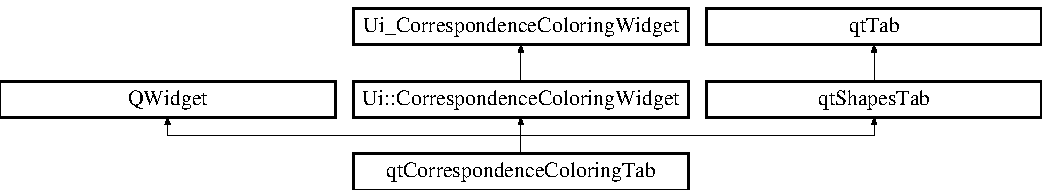
\includegraphics[height=2.557078cm]{classqt_correspondence_coloring_tab}
\end{center}
\end{figure}
\subsection*{Public Member Functions}
\begin{DoxyCompactItemize}
\item 
\hypertarget{classqt_correspondence_coloring_tab_a8f793bb0b1e4fcd2930a6fc8dda03ff4}{}{\bfseries qt\+Correspondence\+Coloring\+Tab} (\hyperlink{class_hash_map}{Hash\+Map}$<$ vtk\+Actor $\ast$, \hyperlink{class_shape}{Shape} $\ast$ $>$ $\ast$map, \hyperlink{class_hash_map}{Hash\+Map}$<$ \hyperlink{class_face_correspondence_data}{Face\+Correspondence\+Data} $\ast$, bool $>$ $\ast$face\+Corr, \hyperlink{class_hash_map}{Hash\+Map}$<$ \hyperlink{class_point_correspondence_data}{Point\+Correspondence\+Data} $\ast$, bool $>$ $\ast$point\+Corr, Q\+Widget $\ast$parent, Qt\+::\+Window\+Flags f=0)\label{classqt_correspondence_coloring_tab_a8f793bb0b1e4fcd2930a6fc8dda03ff4}

\item 
\hypertarget{classqt_correspondence_coloring_tab_a731f7da293d21c87059515a10d36d1e3}{}virtual void {\bfseries on\+Shape\+Delete} (\hyperlink{class_shape}{Shape} $\ast$shape)\label{classqt_correspondence_coloring_tab_a731f7da293d21c87059515a10d36d1e3}

\item 
\hypertarget{classqt_correspondence_coloring_tab_aa42744063025d9b0d29b9a83817c0f27}{}virtual void {\bfseries on\+Shape\+Add} (\hyperlink{class_shape}{Shape} $\ast$shape)\label{classqt_correspondence_coloring_tab_aa42744063025d9b0d29b9a83817c0f27}

\item 
\hypertarget{classqt_correspondence_coloring_tab_a30c174762eda93581d7f93bf4d247788}{}virtual void {\bfseries on\+Shape\+Edit} (\hyperlink{class_shape}{Shape} $\ast$shape)\label{classqt_correspondence_coloring_tab_a30c174762eda93581d7f93bf4d247788}

\item 
\hypertarget{classqt_correspondence_coloring_tab_af02e0bad7197ef2a4fba5e67a6d5f4e2}{}virtual void {\bfseries on\+Shape\+Select} (\hyperlink{class_shape}{Shape} $\ast$shape)\label{classqt_correspondence_coloring_tab_af02e0bad7197ef2a4fba5e67a6d5f4e2}

\item 
\hypertarget{classqt_correspondence_coloring_tab_a3f5f147052eb9b10c08af1160ff85f42}{}virtual void {\bfseries on\+Clear} ()\label{classqt_correspondence_coloring_tab_a3f5f147052eb9b10c08af1160ff85f42}

\end{DoxyCompactItemize}
\subsection*{Additional Inherited Members}


The documentation for this class was generated from the following files\+:\begin{DoxyCompactItemize}
\item 
src/view/qt/qt\+Correspondence\+Coloring\+Tab.\+h\item 
src/view/qt/qt\+Correspondence\+Coloring\+Tab.\+cpp\end{DoxyCompactItemize}

\hypertarget{classqt_correspondences_tab}{}\section{qt\+Correspondences\+Tab Class Reference}
\label{classqt_correspondences_tab}\index{qt\+Correspondences\+Tab@{qt\+Correspondences\+Tab}}
Inheritance diagram for qt\+Correspondences\+Tab\+:\begin{figure}[H]
\begin{center}
\leavevmode
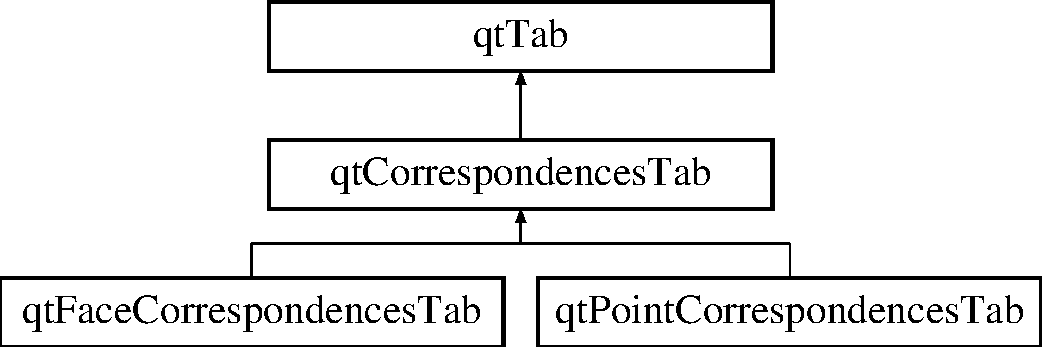
\includegraphics[height=3.000000cm]{classqt_correspondences_tab}
\end{center}
\end{figure}
\subsection*{Public Member Functions}
\begin{DoxyCompactItemize}
\item 
\hypertarget{classqt_correspondences_tab_aeae94691e7d805bd59f55d7089e3877b}{}virtual void {\bfseries on\+Correspondence\+Add} (\hyperlink{class_correspondence_data}{Correspondence\+Data} $\ast$correspondence)=0\label{classqt_correspondences_tab_aeae94691e7d805bd59f55d7089e3877b}

\item 
\hypertarget{classqt_correspondences_tab_a72f76de30e069736cfcebb88327bfd2b}{}virtual void {\bfseries on\+Correspondence\+Delete} (\hyperlink{class_correspondence_data}{Correspondence\+Data} $\ast$correspondence)=0\label{classqt_correspondences_tab_a72f76de30e069736cfcebb88327bfd2b}

\item 
\hypertarget{classqt_correspondences_tab_a2dcdf110605a3248765096b201b96a6b}{}virtual void {\bfseries on\+Correspondence\+Edit} (\hyperlink{class_correspondence}{Correspondence} $\ast$correspondence)=0\label{classqt_correspondences_tab_a2dcdf110605a3248765096b201b96a6b}

\item 
\hypertarget{classqt_correspondences_tab_adabc383fed7b49ed81d98c1a8aedfbab}{}virtual void {\bfseries on\+Correspondence\+Select} (\hyperlink{class_correspondence}{Correspondence} $\ast$correspondence)=0\label{classqt_correspondences_tab_adabc383fed7b49ed81d98c1a8aedfbab}

\item 
\hypertarget{classqt_correspondences_tab_a27b27c974712221e92ce16f2b6dc3661}{}virtual void {\bfseries on\+Point\+Correspondences\+Clear} ()=0\label{classqt_correspondences_tab_a27b27c974712221e92ce16f2b6dc3661}

\item 
\hypertarget{classqt_correspondences_tab_a7f93bc060bfaab22019d910113487356}{}virtual void {\bfseries on\+Face\+Correspondences\+Clear} ()=0\label{classqt_correspondences_tab_a7f93bc060bfaab22019d910113487356}

\end{DoxyCompactItemize}


The documentation for this class was generated from the following file\+:\begin{DoxyCompactItemize}
\item 
src/view/qt/qt\+Correspondences\+Tab.\+h\end{DoxyCompactItemize}

\hypertarget{classqt_face_correspondences_tab}{}\section{qt\+Face\+Correspondences\+Tab Class Reference}
\label{classqt_face_correspondences_tab}\index{qt\+Face\+Correspondences\+Tab@{qt\+Face\+Correspondences\+Tab}}
Inheritance diagram for qt\+Face\+Correspondences\+Tab\+:\begin{figure}[H]
\begin{center}
\leavevmode
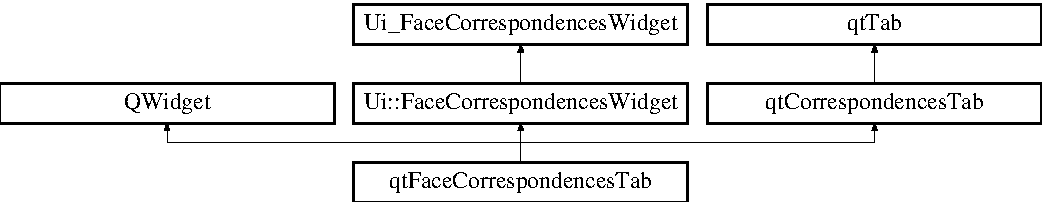
\includegraphics[height=2.718446cm]{classqt_face_correspondences_tab}
\end{center}
\end{figure}
\subsection*{Public Member Functions}
\begin{DoxyCompactItemize}
\item 
\hypertarget{classqt_face_correspondences_tab_a6d8f996f30a0cbd5de5f159e00438f70}{}{\bfseries qt\+Face\+Correspondences\+Tab} (\hyperlink{class_hash_map}{Hash\+Map}$<$ \hyperlink{class_face_correspondence_data}{Face\+Correspondence\+Data} $\ast$, bool $>$ $\ast$face\+Correspondences, \hyperlink{class_shape_analyzer}{Shape\+Analyzer} $\ast$parent, Qt\+::\+Window\+Flags f=0)\label{classqt_face_correspondences_tab_a6d8f996f30a0cbd5de5f159e00438f70}

\item 
\hypertarget{classqt_face_correspondences_tab_a96fe4ebb18a3969b3576dddfffcaf044}{}virtual void {\bfseries on\+Clear} ()\label{classqt_face_correspondences_tab_a96fe4ebb18a3969b3576dddfffcaf044}

\item 
\hypertarget{classqt_face_correspondences_tab_a6e921225a7049a72fe4b24c355892160}{}virtual void {\bfseries on\+Shape\+Delete} (\hyperlink{class_shape}{Shape} $\ast$shape)\label{classqt_face_correspondences_tab_a6e921225a7049a72fe4b24c355892160}

\item 
\hypertarget{classqt_face_correspondences_tab_ac82e5ba6753e031622ef9441a77a21f1}{}virtual void {\bfseries on\+Correspondence\+Add} (\hyperlink{class_correspondence_data}{Correspondence\+Data} $\ast$correspondence)\label{classqt_face_correspondences_tab_ac82e5ba6753e031622ef9441a77a21f1}

\item 
\hypertarget{classqt_face_correspondences_tab_a6baeb2cd594a9cab17964279b09e4184}{}virtual void {\bfseries on\+Correspondence\+Delete} (\hyperlink{class_correspondence_data}{Correspondence\+Data} $\ast$correspondence)\label{classqt_face_correspondences_tab_a6baeb2cd594a9cab17964279b09e4184}

\item 
\hypertarget{classqt_face_correspondences_tab_a97ea9fe1a2a34f3c8d93e07feb5e244f}{}virtual void {\bfseries on\+Correspondence\+Edit} (\hyperlink{class_correspondence}{Correspondence} $\ast$correspondence)\label{classqt_face_correspondences_tab_a97ea9fe1a2a34f3c8d93e07feb5e244f}

\item 
\hypertarget{classqt_face_correspondences_tab_a80bc8351b1d779799bc8ead3606e2226}{}virtual void {\bfseries on\+Correspondence\+Select} (\hyperlink{class_correspondence}{Correspondence} $\ast$correspondence)\label{classqt_face_correspondences_tab_a80bc8351b1d779799bc8ead3606e2226}

\item 
\hypertarget{classqt_face_correspondences_tab_ad269bd09d424447acf38503ba3f4c92d}{}virtual void {\bfseries on\+Point\+Correspondences\+Clear} ()\label{classqt_face_correspondences_tab_ad269bd09d424447acf38503ba3f4c92d}

\item 
\hypertarget{classqt_face_correspondences_tab_a501483fe0ff0919be4596518dd1ff05c}{}virtual void {\bfseries on\+Face\+Correspondences\+Clear} ()\label{classqt_face_correspondences_tab_a501483fe0ff0919be4596518dd1ff05c}

\end{DoxyCompactItemize}
\subsection*{Additional Inherited Members}


The documentation for this class was generated from the following files\+:\begin{DoxyCompactItemize}
\item 
src/view/qt/qt\+Face\+Correspondences\+Tab.\+h\item 
src/view/qt/qt\+Face\+Correspondences\+Tab.\+cpp\end{DoxyCompactItemize}

\hypertarget{classqt_list_widget_item}{}\section{qt\+List\+Widget\+Item$<$ T $>$ Class Template Reference}
\label{classqt_list_widget_item}\index{qt\+List\+Widget\+Item$<$ T $>$@{qt\+List\+Widget\+Item$<$ T $>$}}
Inheritance diagram for qt\+List\+Widget\+Item$<$ T $>$\+:\begin{figure}[H]
\begin{center}
\leavevmode
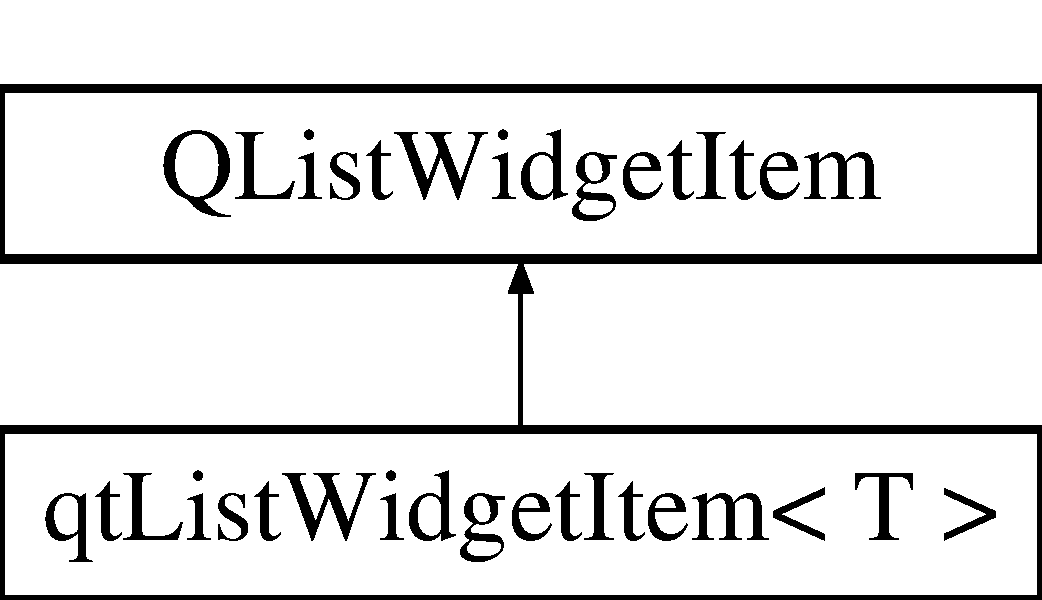
\includegraphics[height=2.000000cm]{classqt_list_widget_item}
\end{center}
\end{figure}
\subsection*{Public Member Functions}
\begin{DoxyCompactItemize}
\item 
\hypertarget{classqt_list_widget_item_a40ae78331ce2548e31b05a5dfe6396b4}{}{\bfseries qt\+List\+Widget\+Item} (const Q\+String \&text, T $\ast$item, Q\+List\+Widget $\ast$view=0, int type=Type)\label{classqt_list_widget_item_a40ae78331ce2548e31b05a5dfe6396b4}

\item 
\hypertarget{classqt_list_widget_item_a008ed2a5dd5c895cd19d96c2040258fd}{}T $\ast$ {\bfseries get\+Item} ()\label{classqt_list_widget_item_a008ed2a5dd5c895cd19d96c2040258fd}

\end{DoxyCompactItemize}


The documentation for this class was generated from the following file\+:\begin{DoxyCompactItemize}
\item 
src/view/qt/qt\+List\+Widget\+Item.\+h\end{DoxyCompactItemize}

\hypertarget{classqt_mesh_check_tab}{}\section{qt\+Mesh\+Check\+Tab Class Reference}
\label{classqt_mesh_check_tab}\index{qt\+Mesh\+Check\+Tab@{qt\+Mesh\+Check\+Tab}}
Inheritance diagram for qt\+Mesh\+Check\+Tab\+:\begin{figure}[H]
\begin{center}
\leavevmode
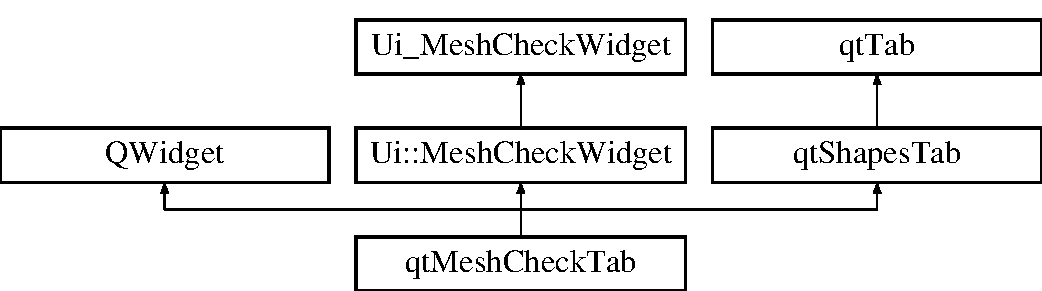
\includegraphics[height=3.000000cm]{classqt_mesh_check_tab}
\end{center}
\end{figure}
\subsection*{Public Member Functions}
\begin{DoxyCompactItemize}
\item 
\hypertarget{classqt_mesh_check_tab_a8a976c8d86aabd648ca0397326b8e730}{}{\bfseries qt\+Mesh\+Check\+Tab} (\hyperlink{class_hash_map}{Hash\+Map}$<$ vtk\+Actor $\ast$, \hyperlink{class_shape}{Shape} $\ast$ $>$ $\ast$shapes, Q\+Widget $\ast$parent, Qt\+::\+Window\+Flags f=0)\label{classqt_mesh_check_tab_a8a976c8d86aabd648ca0397326b8e730}

\item 
virtual void \hyperlink{classqt_mesh_check_tab_aa1f583fbc0604f8c34528efd581e0633}{on\+Shape\+Delete} (\hyperlink{class_shape}{Shape} $\ast$shape)
\begin{DoxyCompactList}\small\item\em Virtual function that triggers when a shape is deleted. \end{DoxyCompactList}\item 
virtual void \hyperlink{classqt_mesh_check_tab_a8182eeedc7be66ea9d377011ace81125}{on\+Shape\+Add} (\hyperlink{class_shape}{Shape} $\ast$shape)
\begin{DoxyCompactList}\small\item\em Virtual trigger function for new shapes. \end{DoxyCompactList}\item 
virtual void \hyperlink{classqt_mesh_check_tab_a01aea7b3fd612932b7a19b244b4b44a0}{on\+Shape\+Edit} (\hyperlink{class_shape}{Shape} $\ast$shape)
\begin{DoxyCompactList}\small\item\em Virtual trigger function for edited shapes. \end{DoxyCompactList}\item 
virtual void \hyperlink{classqt_mesh_check_tab_a72ed8ca09f9100689a41dec77523bf4e}{on\+Shape\+Select} (\hyperlink{class_shape}{Shape} $\ast$shape)
\begin{DoxyCompactList}\small\item\em Virtual trigger function for selecting shapes. \end{DoxyCompactList}\item 
virtual void \hyperlink{classqt_mesh_check_tab_a5ca41a6c3c905f572632a2b754f86b7c}{on\+Clear} ()
\begin{DoxyCompactList}\small\item\em Virtual function that triggers when the app is cleared. \end{DoxyCompactList}\end{DoxyCompactItemize}
\subsection*{Additional Inherited Members}


\subsection{Member Function Documentation}
\hypertarget{classqt_mesh_check_tab_a5ca41a6c3c905f572632a2b754f86b7c}{}\index{qt\+Mesh\+Check\+Tab@{qt\+Mesh\+Check\+Tab}!on\+Clear@{on\+Clear}}
\index{on\+Clear@{on\+Clear}!qt\+Mesh\+Check\+Tab@{qt\+Mesh\+Check\+Tab}}
\subsubsection[{on\+Clear}]{\setlength{\rightskip}{0pt plus 5cm}void qt\+Mesh\+Check\+Tab\+::on\+Clear (
\begin{DoxyParamCaption}
{}
\end{DoxyParamCaption}
)\hspace{0.3cm}{\ttfamily [virtual]}}\label{classqt_mesh_check_tab_a5ca41a6c3c905f572632a2b754f86b7c}


Virtual function that triggers when the app is cleared. 

The function is triggered before any objects are deleted from the G\+U\+I or other data structures in the main application. 

Implements \hyperlink{classqt_tab_aeca48d82349df4c61fbfb66c4273c9b6}{qt\+Tab}.

\hypertarget{classqt_mesh_check_tab_a8182eeedc7be66ea9d377011ace81125}{}\index{qt\+Mesh\+Check\+Tab@{qt\+Mesh\+Check\+Tab}!on\+Shape\+Add@{on\+Shape\+Add}}
\index{on\+Shape\+Add@{on\+Shape\+Add}!qt\+Mesh\+Check\+Tab@{qt\+Mesh\+Check\+Tab}}
\subsubsection[{on\+Shape\+Add}]{\setlength{\rightskip}{0pt plus 5cm}void qt\+Mesh\+Check\+Tab\+::on\+Shape\+Add (
\begin{DoxyParamCaption}
\item[{{\bf Shape} $\ast$}]{shape}
\end{DoxyParamCaption}
)\hspace{0.3cm}{\ttfamily [virtual]}}\label{classqt_mesh_check_tab_a8182eeedc7be66ea9d377011ace81125}


Virtual trigger function for new shapes. 

The function is triggered before the shape is added to the G\+U\+I or included in any data structures in the main application. 
\begin{DoxyParams}{Parameters}
{\em shape} & Pointer to added shape. \\
\hline
\end{DoxyParams}


Implements \hyperlink{classqt_shapes_tab_ac1785d1af606cd4ae0cd29708af7ae6f}{qt\+Shapes\+Tab}.

\hypertarget{classqt_mesh_check_tab_aa1f583fbc0604f8c34528efd581e0633}{}\index{qt\+Mesh\+Check\+Tab@{qt\+Mesh\+Check\+Tab}!on\+Shape\+Delete@{on\+Shape\+Delete}}
\index{on\+Shape\+Delete@{on\+Shape\+Delete}!qt\+Mesh\+Check\+Tab@{qt\+Mesh\+Check\+Tab}}
\subsubsection[{on\+Shape\+Delete}]{\setlength{\rightskip}{0pt plus 5cm}void qt\+Mesh\+Check\+Tab\+::on\+Shape\+Delete (
\begin{DoxyParamCaption}
\item[{{\bf Shape} $\ast$}]{shape}
\end{DoxyParamCaption}
)\hspace{0.3cm}{\ttfamily [virtual]}}\label{classqt_mesh_check_tab_aa1f583fbc0604f8c34528efd581e0633}


Virtual function that triggers when a shape is deleted. 

The function is triggered before it is actually deleted from the G\+U\+I or other data structures in the main application. 
\begin{DoxyParams}{Parameters}
{\em shape} & Pointer to the shape that is deleted. \\
\hline
\end{DoxyParams}


Implements \hyperlink{classqt_tab_a8811879f2aaf15777025427eec7b9fd9}{qt\+Tab}.

\hypertarget{classqt_mesh_check_tab_a01aea7b3fd612932b7a19b244b4b44a0}{}\index{qt\+Mesh\+Check\+Tab@{qt\+Mesh\+Check\+Tab}!on\+Shape\+Edit@{on\+Shape\+Edit}}
\index{on\+Shape\+Edit@{on\+Shape\+Edit}!qt\+Mesh\+Check\+Tab@{qt\+Mesh\+Check\+Tab}}
\subsubsection[{on\+Shape\+Edit}]{\setlength{\rightskip}{0pt plus 5cm}void qt\+Mesh\+Check\+Tab\+::on\+Shape\+Edit (
\begin{DoxyParamCaption}
\item[{{\bf Shape} $\ast$}]{shape}
\end{DoxyParamCaption}
)\hspace{0.3cm}{\ttfamily [virtual]}}\label{classqt_mesh_check_tab_a01aea7b3fd612932b7a19b244b4b44a0}


Virtual trigger function for edited shapes. 


\begin{DoxyParams}{Parameters}
{\em shape} & Pointer to edited shape. \\
\hline
\end{DoxyParams}


Implements \hyperlink{classqt_shapes_tab_a7e6ef278c299ef8934b6c1164b90574a}{qt\+Shapes\+Tab}.

\hypertarget{classqt_mesh_check_tab_a72ed8ca09f9100689a41dec77523bf4e}{}\index{qt\+Mesh\+Check\+Tab@{qt\+Mesh\+Check\+Tab}!on\+Shape\+Select@{on\+Shape\+Select}}
\index{on\+Shape\+Select@{on\+Shape\+Select}!qt\+Mesh\+Check\+Tab@{qt\+Mesh\+Check\+Tab}}
\subsubsection[{on\+Shape\+Select}]{\setlength{\rightskip}{0pt plus 5cm}void qt\+Mesh\+Check\+Tab\+::on\+Shape\+Select (
\begin{DoxyParamCaption}
\item[{{\bf Shape} $\ast$}]{shape}
\end{DoxyParamCaption}
)\hspace{0.3cm}{\ttfamily [virtual]}}\label{classqt_mesh_check_tab_a72ed8ca09f9100689a41dec77523bf4e}


Virtual trigger function for selecting shapes. 


\begin{DoxyParams}{Parameters}
{\em shape} & Pointer to selected shape. \\
\hline
\end{DoxyParams}


Implements \hyperlink{classqt_shapes_tab_a50992777c7c5bcdf31adbb23e6bfb3a5}{qt\+Shapes\+Tab}.



The documentation for this class was generated from the following files\+:\begin{DoxyCompactItemize}
\item 
src/view/qt/qt\+Mesh\+Check\+Tab.\+h\item 
src/view/qt/qt\+Mesh\+Check\+Tab.\+cpp\end{DoxyCompactItemize}

\hypertarget{classqt_point_correspondences_tab}{}\section{qt\+Point\+Correspondences\+Tab Class Reference}
\label{classqt_point_correspondences_tab}\index{qt\+Point\+Correspondences\+Tab@{qt\+Point\+Correspondences\+Tab}}
Inheritance diagram for qt\+Point\+Correspondences\+Tab\+:\begin{figure}[H]
\begin{center}
\leavevmode
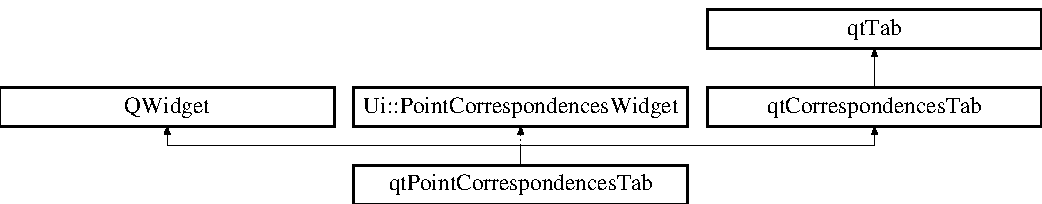
\includegraphics[height=2.745098cm]{classqt_point_correspondences_tab}
\end{center}
\end{figure}
\subsection*{Public Member Functions}
\begin{DoxyCompactItemize}
\item 
\hypertarget{classqt_point_correspondences_tab_a846ba4575f7b2acf1c4d6bf969a1058a}{}{\bfseries qt\+Point\+Correspondences\+Tab} (\hyperlink{class_hash_map}{Hash\+Map}$<$ \hyperlink{class_point_correspondence_data}{Point\+Correspondence\+Data} $\ast$, bool $>$ $\ast$point\+Correspondences, \hyperlink{class_shape_analyzer}{Shape\+Analyzer} $\ast$parent, Qt\+::\+Window\+Flags f=0)\label{classqt_point_correspondences_tab_a846ba4575f7b2acf1c4d6bf969a1058a}

\item 
\hypertarget{classqt_point_correspondences_tab_a7e07cc3dbe7981215885d5b9ddab14a8}{}virtual void {\bfseries on\+Clear} ()\label{classqt_point_correspondences_tab_a7e07cc3dbe7981215885d5b9ddab14a8}

\item 
\hypertarget{classqt_point_correspondences_tab_a3fd3d809d1686a5397befe85feeac399}{}virtual void {\bfseries on\+Shape\+Delete} (\hyperlink{class_shape}{Shape} $\ast$shape)\label{classqt_point_correspondences_tab_a3fd3d809d1686a5397befe85feeac399}

\item 
\hypertarget{classqt_point_correspondences_tab_abd778bdd1cac74a256c487e396c1b91c}{}virtual void {\bfseries on\+Correspondence\+Add} (\hyperlink{class_correspondence_data}{Correspondence\+Data} $\ast$correspondence)\label{classqt_point_correspondences_tab_abd778bdd1cac74a256c487e396c1b91c}

\item 
\hypertarget{classqt_point_correspondences_tab_a4cce7bd311c4d4076cdb62c77526b913}{}virtual void {\bfseries on\+Correspondence\+Delete} (\hyperlink{class_correspondence_data}{Correspondence\+Data} $\ast$correspondence)\label{classqt_point_correspondences_tab_a4cce7bd311c4d4076cdb62c77526b913}

\item 
\hypertarget{classqt_point_correspondences_tab_a31bacf4fea3333cbd8bcc1fc04e67d02}{}virtual void {\bfseries on\+Correspondence\+Edit} (\hyperlink{class_correspondence}{Correspondence} $\ast$correspondence)\label{classqt_point_correspondences_tab_a31bacf4fea3333cbd8bcc1fc04e67d02}

\item 
\hypertarget{classqt_point_correspondences_tab_a3cdbc161275ce825fcf5833b1c5ef2e1}{}virtual void {\bfseries on\+Correspondence\+Select} (\hyperlink{class_correspondence}{Correspondence} $\ast$correspondence)\label{classqt_point_correspondences_tab_a3cdbc161275ce825fcf5833b1c5ef2e1}

\item 
\hypertarget{classqt_point_correspondences_tab_a45ce09045bb6c497f8b819e8929b3716}{}virtual void {\bfseries on\+Point\+Correspondences\+Clear} ()\label{classqt_point_correspondences_tab_a45ce09045bb6c497f8b819e8929b3716}

\item 
\hypertarget{classqt_point_correspondences_tab_a305e25d4b740d51af1a6d60c37bf8668}{}virtual void {\bfseries on\+Face\+Correspondences\+Clear} ()\label{classqt_point_correspondences_tab_a305e25d4b740d51af1a6d60c37bf8668}

\end{DoxyCompactItemize}


The documentation for this class was generated from the following files\+:\begin{DoxyCompactItemize}
\item 
src/view/qt/qt\+Point\+Correspondences\+Tab.\+h\item 
src/view/qt/qt\+Point\+Correspondence\+Tab.\+cpp\end{DoxyCompactItemize}

\hypertarget{classqt_shape_info_tab}{}\section{qt\+Shape\+Info\+Tab Class Reference}
\label{classqt_shape_info_tab}\index{qt\+Shape\+Info\+Tab@{qt\+Shape\+Info\+Tab}}


Tab that shows basic information about the selected shape.  




{\ttfamily \#include $<$qt\+Shape\+Info\+Tab.\+h$>$}

Inheritance diagram for qt\+Shape\+Info\+Tab\+:\begin{figure}[H]
\begin{center}
\leavevmode
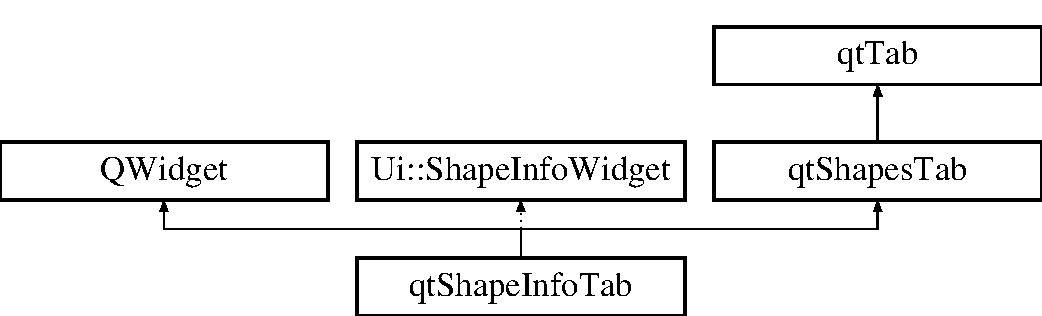
\includegraphics[height=3.000000cm]{classqt_shape_info_tab}
\end{center}
\end{figure}
\subsection*{Public Member Functions}
\begin{DoxyCompactItemize}
\item 
\hypertarget{classqt_shape_info_tab_a1e24b3b05a98ebf3aec79cd7c0c3e8ba}{}\hyperlink{classqt_shape_info_tab_a1e24b3b05a98ebf3aec79cd7c0c3e8ba}{qt\+Shape\+Info\+Tab} (Q\+Widget $\ast$parent, Qt\+::\+Window\+Flags f=0)\label{classqt_shape_info_tab_a1e24b3b05a98ebf3aec79cd7c0c3e8ba}

\begin{DoxyCompactList}\small\item\em Initializes an empty tab. \end{DoxyCompactList}\item 
\hypertarget{classqt_shape_info_tab_ad110fe4c0e748e126ee030a078714b72}{}\hyperlink{classqt_shape_info_tab_ad110fe4c0e748e126ee030a078714b72}{qt\+Shape\+Info\+Tab} (\hyperlink{class_shape}{Shape} $\ast$shape, Q\+Widget $\ast$parent, Qt\+::\+Window\+Flags f=0)\label{classqt_shape_info_tab_ad110fe4c0e748e126ee030a078714b72}

\begin{DoxyCompactList}\small\item\em Initializes an tab with information about the given shape. \end{DoxyCompactList}\end{DoxyCompactItemize}
\begin{Indent}{\bf qt\+Tab / qt\+Shapes\+Tab Functions}\par
{\em Implements abstract functions of \hyperlink{classqt_tab}{qt\+Tab} and \hyperlink{classqt_shapes_tab}{qt\+Shapes\+Tab}.

Clears all content from the tab. }\begin{DoxyCompactItemize}
\item 
virtual void \hyperlink{classqt_shape_info_tab_a295e58538f2cebdfd9a4b5b40bf1e16c}{on\+Shape\+Delete} (\hyperlink{class_shape}{Shape} $\ast$shape)
\begin{DoxyCompactList}\small\item\em Virtual function that triggers when a shape is deleted. \end{DoxyCompactList}\item 
\hypertarget{classqt_shape_info_tab_aec9838aa8baceca3a6045b5950e2881d}{}virtual void \hyperlink{classqt_shape_info_tab_aec9838aa8baceca3a6045b5950e2881d}{on\+Shape\+Add} (\hyperlink{class_shape}{Shape} $\ast$shape)\label{classqt_shape_info_tab_aec9838aa8baceca3a6045b5950e2881d}

\begin{DoxyCompactList}\small\item\em Empty. \end{DoxyCompactList}\item 
virtual void \hyperlink{classqt_shape_info_tab_acc7e4b91ec5eff4e8a785730a21a44f8}{on\+Shape\+Edit} (\hyperlink{class_shape}{Shape} $\ast$shape)
\begin{DoxyCompactList}\small\item\em Updates the information if the edited shapes was the selected one. \end{DoxyCompactList}\item 
\hypertarget{classqt_shape_info_tab_a785dda79e10dfd05845e08ab1b4cdfd9}{}virtual void \hyperlink{classqt_shape_info_tab_a785dda79e10dfd05845e08ab1b4cdfd9}{on\+Shape\+Select} (\hyperlink{class_shape}{Shape} $\ast$shape)\label{classqt_shape_info_tab_a785dda79e10dfd05845e08ab1b4cdfd9}

\begin{DoxyCompactList}\small\item\em Updates the tab to show information for the new selected shape. \end{DoxyCompactList}\item 
\hypertarget{classqt_shape_info_tab_ae7f1b60ab068ec55b67830742e7534d8}{}virtual void \hyperlink{classqt_shape_info_tab_ae7f1b60ab068ec55b67830742e7534d8}{on\+Clear} ()\label{classqt_shape_info_tab_ae7f1b60ab068ec55b67830742e7534d8}

\begin{DoxyCompactList}\small\item\em Clears all content from the tab. \end{DoxyCompactList}\end{DoxyCompactItemize}
\end{Indent}


\subsection{Detailed Description}
Tab that shows basic information about the selected shape. 

\begin{DoxyAuthor}{Author}
Zorah Lähner 
\end{DoxyAuthor}


\subsection{Member Function Documentation}
\hypertarget{classqt_shape_info_tab_a295e58538f2cebdfd9a4b5b40bf1e16c}{}\index{qt\+Shape\+Info\+Tab@{qt\+Shape\+Info\+Tab}!on\+Shape\+Delete@{on\+Shape\+Delete}}
\index{on\+Shape\+Delete@{on\+Shape\+Delete}!qt\+Shape\+Info\+Tab@{qt\+Shape\+Info\+Tab}}
\subsubsection[{on\+Shape\+Delete}]{\setlength{\rightskip}{0pt plus 5cm}void qt\+Shape\+Info\+Tab\+::on\+Shape\+Delete (
\begin{DoxyParamCaption}
\item[{{\bf Shape} $\ast$}]{shape}
\end{DoxyParamCaption}
)\hspace{0.3cm}{\ttfamily [virtual]}}\label{classqt_shape_info_tab_a295e58538f2cebdfd9a4b5b40bf1e16c}


Virtual function that triggers when a shape is deleted. 

The function is triggered before it is actually deleted from the G\+U\+I or other data structures in the main application. 
\begin{DoxyParams}{Parameters}
{\em shape} & Pointer to the shape that is deleted. \\
\hline
\end{DoxyParams}


Implements \hyperlink{classqt_tab_a8811879f2aaf15777025427eec7b9fd9}{qt\+Tab}.

\hypertarget{classqt_shape_info_tab_acc7e4b91ec5eff4e8a785730a21a44f8}{}\index{qt\+Shape\+Info\+Tab@{qt\+Shape\+Info\+Tab}!on\+Shape\+Edit@{on\+Shape\+Edit}}
\index{on\+Shape\+Edit@{on\+Shape\+Edit}!qt\+Shape\+Info\+Tab@{qt\+Shape\+Info\+Tab}}
\subsubsection[{on\+Shape\+Edit}]{\setlength{\rightskip}{0pt plus 5cm}void qt\+Shape\+Info\+Tab\+::on\+Shape\+Edit (
\begin{DoxyParamCaption}
\item[{{\bf Shape} $\ast$}]{shape}
\end{DoxyParamCaption}
)\hspace{0.3cm}{\ttfamily [virtual]}}\label{classqt_shape_info_tab_acc7e4b91ec5eff4e8a785730a21a44f8}


Updates the information if the edited shapes was the selected one. 

The only possible changing information is the name at the moment. Other entries will not be updated. \begin{DoxyNote}{Note}
If further editing of shapes is implemented later on, this function has to be updated. 
\end{DoxyNote}


Implements \hyperlink{classqt_shapes_tab_a7e6ef278c299ef8934b6c1164b90574a}{qt\+Shapes\+Tab}.



The documentation for this class was generated from the following files\+:\begin{DoxyCompactItemize}
\item 
src/view/qt/qt\+Shape\+Info\+Tab.\+h\item 
src/view/qt/qt\+Shape\+Info\+Tab.\+cpp\end{DoxyCompactItemize}

\hypertarget{classqt_shape_interpolation_tab}{}\section{qt\+Shape\+Interpolation\+Tab Class Reference}
\label{classqt_shape_interpolation_tab}\index{qt\+Shape\+Interpolation\+Tab@{qt\+Shape\+Interpolation\+Tab}}
Inheritance diagram for qt\+Shape\+Interpolation\+Tab\+:\begin{figure}[H]
\begin{center}
\leavevmode
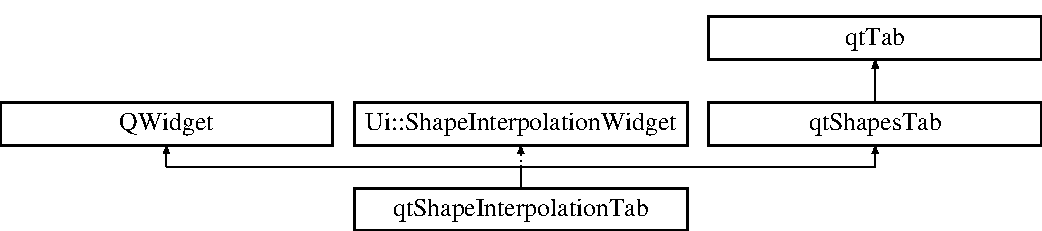
\includegraphics[height=3.000000cm]{classqt_shape_interpolation_tab}
\end{center}
\end{figure}
\subsection*{Public Member Functions}
\begin{DoxyCompactItemize}
\item 
\hypertarget{classqt_shape_interpolation_tab_a81e12bc1650f508da0a30903a5ee54d5}{}{\bfseries qt\+Shape\+Interpolation\+Tab} (\hyperlink{class_hash_map}{Hash\+Map}$<$ vtk\+Actor $\ast$, \hyperlink{class_shape}{Shape} $\ast$ $>$ $\ast$shapes, \hyperlink{class_hash_map}{Hash\+Map}$<$ \hyperlink{class_point_correspondence_data}{Point\+Correspondence\+Data} $\ast$, bool $>$ $\ast$correspondences, vtk\+Smart\+Pointer$<$ vtk\+Renderer $>$ renderer, int \&last\+Insert\+Shape\+I\+D, \hyperlink{class_shape_analyzer}{Shape\+Analyzer} $\ast$parent, Qt\+::\+Window\+Flags f=0)\label{classqt_shape_interpolation_tab_a81e12bc1650f508da0a30903a5ee54d5}

\item 
virtual void \hyperlink{classqt_shape_interpolation_tab_aac6776b2f521abe2d9aa6f932665cf57}{on\+Shape\+Delete} (\hyperlink{class_shape}{Shape} $\ast$shape)
\begin{DoxyCompactList}\small\item\em Virtual function that triggers when a shape is deleted. \end{DoxyCompactList}\item 
virtual void \hyperlink{classqt_shape_interpolation_tab_a9801bcf3d2e1b31a79824d8b623e1762}{on\+Shape\+Add} (\hyperlink{class_shape}{Shape} $\ast$shape)
\begin{DoxyCompactList}\small\item\em Virtual trigger function for new shapes. \end{DoxyCompactList}\item 
virtual void \hyperlink{classqt_shape_interpolation_tab_a556d7b2a445f0cd5f6a5fd1f912d144a}{on\+Shape\+Edit} (\hyperlink{class_shape}{Shape} $\ast$shape)
\begin{DoxyCompactList}\small\item\em Virtual trigger function for edited shapes. \end{DoxyCompactList}\item 
virtual void \hyperlink{classqt_shape_interpolation_tab_a4db77c18d8b2257ac14654ef7c9f5ecd}{on\+Shape\+Select} (\hyperlink{class_shape}{Shape} $\ast$shape)
\begin{DoxyCompactList}\small\item\em Virtual trigger function for selecting shapes. \end{DoxyCompactList}\item 
virtual void \hyperlink{classqt_shape_interpolation_tab_a71ad9a70adc5408de4ceb94467953d8c}{on\+Clear} ()
\begin{DoxyCompactList}\small\item\em Virtual function that triggers when the app is cleared. \end{DoxyCompactList}\end{DoxyCompactItemize}


\subsection{Member Function Documentation}
\hypertarget{classqt_shape_interpolation_tab_a71ad9a70adc5408de4ceb94467953d8c}{}\index{qt\+Shape\+Interpolation\+Tab@{qt\+Shape\+Interpolation\+Tab}!on\+Clear@{on\+Clear}}
\index{on\+Clear@{on\+Clear}!qt\+Shape\+Interpolation\+Tab@{qt\+Shape\+Interpolation\+Tab}}
\subsubsection[{on\+Clear}]{\setlength{\rightskip}{0pt plus 5cm}void qt\+Shape\+Interpolation\+Tab\+::on\+Clear (
\begin{DoxyParamCaption}
{}
\end{DoxyParamCaption}
)\hspace{0.3cm}{\ttfamily [virtual]}}\label{classqt_shape_interpolation_tab_a71ad9a70adc5408de4ceb94467953d8c}


Virtual function that triggers when the app is cleared. 

The function is triggered before any objects are deleted from the G\+U\+I or other data structures in the main application. 

Implements \hyperlink{classqt_tab_aeca48d82349df4c61fbfb66c4273c9b6}{qt\+Tab}.

\hypertarget{classqt_shape_interpolation_tab_a9801bcf3d2e1b31a79824d8b623e1762}{}\index{qt\+Shape\+Interpolation\+Tab@{qt\+Shape\+Interpolation\+Tab}!on\+Shape\+Add@{on\+Shape\+Add}}
\index{on\+Shape\+Add@{on\+Shape\+Add}!qt\+Shape\+Interpolation\+Tab@{qt\+Shape\+Interpolation\+Tab}}
\subsubsection[{on\+Shape\+Add}]{\setlength{\rightskip}{0pt plus 5cm}void qt\+Shape\+Interpolation\+Tab\+::on\+Shape\+Add (
\begin{DoxyParamCaption}
\item[{{\bf Shape} $\ast$}]{shape}
\end{DoxyParamCaption}
)\hspace{0.3cm}{\ttfamily [virtual]}}\label{classqt_shape_interpolation_tab_a9801bcf3d2e1b31a79824d8b623e1762}


Virtual trigger function for new shapes. 

The function is triggered before the shape is added to the G\+U\+I or included in any data structures in the main application. 
\begin{DoxyParams}{Parameters}
{\em shape} & Pointer to added shape. \\
\hline
\end{DoxyParams}


Implements \hyperlink{classqt_shapes_tab_ac1785d1af606cd4ae0cd29708af7ae6f}{qt\+Shapes\+Tab}.

\hypertarget{classqt_shape_interpolation_tab_aac6776b2f521abe2d9aa6f932665cf57}{}\index{qt\+Shape\+Interpolation\+Tab@{qt\+Shape\+Interpolation\+Tab}!on\+Shape\+Delete@{on\+Shape\+Delete}}
\index{on\+Shape\+Delete@{on\+Shape\+Delete}!qt\+Shape\+Interpolation\+Tab@{qt\+Shape\+Interpolation\+Tab}}
\subsubsection[{on\+Shape\+Delete}]{\setlength{\rightskip}{0pt plus 5cm}void qt\+Shape\+Interpolation\+Tab\+::on\+Shape\+Delete (
\begin{DoxyParamCaption}
\item[{{\bf Shape} $\ast$}]{shape}
\end{DoxyParamCaption}
)\hspace{0.3cm}{\ttfamily [virtual]}}\label{classqt_shape_interpolation_tab_aac6776b2f521abe2d9aa6f932665cf57}


Virtual function that triggers when a shape is deleted. 

The function is triggered before it is actually deleted from the G\+U\+I or other data structures in the main application. 
\begin{DoxyParams}{Parameters}
{\em shape} & Pointer to the shape that is deleted. \\
\hline
\end{DoxyParams}


Implements \hyperlink{classqt_tab_a8811879f2aaf15777025427eec7b9fd9}{qt\+Tab}.

\hypertarget{classqt_shape_interpolation_tab_a556d7b2a445f0cd5f6a5fd1f912d144a}{}\index{qt\+Shape\+Interpolation\+Tab@{qt\+Shape\+Interpolation\+Tab}!on\+Shape\+Edit@{on\+Shape\+Edit}}
\index{on\+Shape\+Edit@{on\+Shape\+Edit}!qt\+Shape\+Interpolation\+Tab@{qt\+Shape\+Interpolation\+Tab}}
\subsubsection[{on\+Shape\+Edit}]{\setlength{\rightskip}{0pt plus 5cm}void qt\+Shape\+Interpolation\+Tab\+::on\+Shape\+Edit (
\begin{DoxyParamCaption}
\item[{{\bf Shape} $\ast$}]{shape}
\end{DoxyParamCaption}
)\hspace{0.3cm}{\ttfamily [virtual]}}\label{classqt_shape_interpolation_tab_a556d7b2a445f0cd5f6a5fd1f912d144a}


Virtual trigger function for edited shapes. 


\begin{DoxyParams}{Parameters}
{\em shape} & Pointer to edited shape. \\
\hline
\end{DoxyParams}


Implements \hyperlink{classqt_shapes_tab_a7e6ef278c299ef8934b6c1164b90574a}{qt\+Shapes\+Tab}.

\hypertarget{classqt_shape_interpolation_tab_a4db77c18d8b2257ac14654ef7c9f5ecd}{}\index{qt\+Shape\+Interpolation\+Tab@{qt\+Shape\+Interpolation\+Tab}!on\+Shape\+Select@{on\+Shape\+Select}}
\index{on\+Shape\+Select@{on\+Shape\+Select}!qt\+Shape\+Interpolation\+Tab@{qt\+Shape\+Interpolation\+Tab}}
\subsubsection[{on\+Shape\+Select}]{\setlength{\rightskip}{0pt plus 5cm}void qt\+Shape\+Interpolation\+Tab\+::on\+Shape\+Select (
\begin{DoxyParamCaption}
\item[{{\bf Shape} $\ast$}]{shape}
\end{DoxyParamCaption}
)\hspace{0.3cm}{\ttfamily [virtual]}}\label{classqt_shape_interpolation_tab_a4db77c18d8b2257ac14654ef7c9f5ecd}


Virtual trigger function for selecting shapes. 


\begin{DoxyParams}{Parameters}
{\em shape} & Pointer to selected shape. \\
\hline
\end{DoxyParams}


Implements \hyperlink{classqt_shapes_tab_a50992777c7c5bcdf31adbb23e6bfb3a5}{qt\+Shapes\+Tab}.



The documentation for this class was generated from the following files\+:\begin{DoxyCompactItemize}
\item 
src/view/qt/qt\+Shape\+Interpolation\+Tab.\+h\item 
src/view/qt/qt\+Shape\+Interpolation\+Tab.\+cpp\end{DoxyCompactItemize}

\hypertarget{classqt_shapes_tab}{}\section{qt\+Shapes\+Tab Class Reference}
\label{classqt_shapes_tab}\index{qt\+Shapes\+Tab@{qt\+Shapes\+Tab}}


Abstract class for Tabs that include Shapes.  




{\ttfamily \#include $<$qt\+Shapes\+Tab.\+h$>$}

Inheritance diagram for qt\+Shapes\+Tab\+:\begin{figure}[H]
\begin{center}
\leavevmode
\includegraphics[height=2.176166cm]{classqt_shapes_tab}
\end{center}
\end{figure}
\subsection*{Public Member Functions}
\begin{DoxyCompactItemize}
\item 
\hypertarget{classqt_shapes_tab_a592ecb3f59fb56e5c978aea874bd9f90}{}virtual \hyperlink{classqt_shapes_tab_a592ecb3f59fb56e5c978aea874bd9f90}{$\sim$qt\+Shapes\+Tab} ()\label{classqt_shapes_tab_a592ecb3f59fb56e5c978aea874bd9f90}

\begin{DoxyCompactList}\small\item\em Virtual Destructor. \end{DoxyCompactList}\item 
virtual void \hyperlink{classqt_shapes_tab_ac1785d1af606cd4ae0cd29708af7ae6f}{on\+Shape\+Add} (\hyperlink{class_shape}{Shape} $\ast$shape)=0
\begin{DoxyCompactList}\small\item\em Virtual trigger function for new shapes. \end{DoxyCompactList}\item 
virtual void \hyperlink{classqt_shapes_tab_a7e6ef278c299ef8934b6c1164b90574a}{on\+Shape\+Edit} (\hyperlink{class_shape}{Shape} $\ast$shape)=0
\begin{DoxyCompactList}\small\item\em Virtual trigger function for edited shapes. \end{DoxyCompactList}\item 
virtual void \hyperlink{classqt_shapes_tab_a50992777c7c5bcdf31adbb23e6bfb3a5}{on\+Shape\+Select} (\hyperlink{class_shape}{Shape} $\ast$shape)=0
\begin{DoxyCompactList}\small\item\em Virtual trigger function for selecting shapes. \end{DoxyCompactList}\end{DoxyCompactItemize}


\subsection{Detailed Description}
Abstract class for Tabs that include Shapes. 

Defines the trigger functions for new shapes, shapes changes and shape selection. Any tab that has to be updated in these events must inherit from this class.

\begin{DoxyAuthor}{Author}
Emanuel Laude 
\end{DoxyAuthor}


\subsection{Member Function Documentation}
\hypertarget{classqt_shapes_tab_ac1785d1af606cd4ae0cd29708af7ae6f}{}\index{qt\+Shapes\+Tab@{qt\+Shapes\+Tab}!on\+Shape\+Add@{on\+Shape\+Add}}
\index{on\+Shape\+Add@{on\+Shape\+Add}!qt\+Shapes\+Tab@{qt\+Shapes\+Tab}}
\subsubsection[{on\+Shape\+Add}]{\setlength{\rightskip}{0pt plus 5cm}virtual void qt\+Shapes\+Tab\+::on\+Shape\+Add (
\begin{DoxyParamCaption}
\item[{{\bf Shape} $\ast$}]{shape}
\end{DoxyParamCaption}
)\hspace{0.3cm}{\ttfamily [pure virtual]}}\label{classqt_shapes_tab_ac1785d1af606cd4ae0cd29708af7ae6f}


Virtual trigger function for new shapes. 

The function is triggered before the shape is added to the G\+U\+I or included in any data structures in the main application. 
\begin{DoxyParams}{Parameters}
{\em shape} & Pointer to added shape. \\
\hline
\end{DoxyParams}


Implemented in \hyperlink{classqt_correspondence_coloring_tab_aa42744063025d9b0d29b9a83817c0f27}{qt\+Correspondence\+Coloring\+Tab}, \hyperlink{classqt_shape_info_tab_aec9838aa8baceca3a6045b5950e2881d}{qt\+Shape\+Info\+Tab}, \hyperlink{classqt_shape_interpolation_tab_a9801bcf3d2e1b31a79824d8b623e1762}{qt\+Shape\+Interpolation\+Tab}, and \hyperlink{classqt_mesh_check_tab_a8182eeedc7be66ea9d377011ace81125}{qt\+Mesh\+Check\+Tab}.

\hypertarget{classqt_shapes_tab_a7e6ef278c299ef8934b6c1164b90574a}{}\index{qt\+Shapes\+Tab@{qt\+Shapes\+Tab}!on\+Shape\+Edit@{on\+Shape\+Edit}}
\index{on\+Shape\+Edit@{on\+Shape\+Edit}!qt\+Shapes\+Tab@{qt\+Shapes\+Tab}}
\subsubsection[{on\+Shape\+Edit}]{\setlength{\rightskip}{0pt plus 5cm}virtual void qt\+Shapes\+Tab\+::on\+Shape\+Edit (
\begin{DoxyParamCaption}
\item[{{\bf Shape} $\ast$}]{shape}
\end{DoxyParamCaption}
)\hspace{0.3cm}{\ttfamily [pure virtual]}}\label{classqt_shapes_tab_a7e6ef278c299ef8934b6c1164b90574a}


Virtual trigger function for edited shapes. 


\begin{DoxyParams}{Parameters}
{\em shape} & Pointer to edited shape. \\
\hline
\end{DoxyParams}


Implemented in \hyperlink{classqt_correspondence_coloring_tab_a30c174762eda93581d7f93bf4d247788}{qt\+Correspondence\+Coloring\+Tab}, \hyperlink{classqt_shape_info_tab_acc7e4b91ec5eff4e8a785730a21a44f8}{qt\+Shape\+Info\+Tab}, \hyperlink{classqt_shape_interpolation_tab_a556d7b2a445f0cd5f6a5fd1f912d144a}{qt\+Shape\+Interpolation\+Tab}, and \hyperlink{classqt_mesh_check_tab_a01aea7b3fd612932b7a19b244b4b44a0}{qt\+Mesh\+Check\+Tab}.

\hypertarget{classqt_shapes_tab_a50992777c7c5bcdf31adbb23e6bfb3a5}{}\index{qt\+Shapes\+Tab@{qt\+Shapes\+Tab}!on\+Shape\+Select@{on\+Shape\+Select}}
\index{on\+Shape\+Select@{on\+Shape\+Select}!qt\+Shapes\+Tab@{qt\+Shapes\+Tab}}
\subsubsection[{on\+Shape\+Select}]{\setlength{\rightskip}{0pt plus 5cm}virtual void qt\+Shapes\+Tab\+::on\+Shape\+Select (
\begin{DoxyParamCaption}
\item[{{\bf Shape} $\ast$}]{shape}
\end{DoxyParamCaption}
)\hspace{0.3cm}{\ttfamily [pure virtual]}}\label{classqt_shapes_tab_a50992777c7c5bcdf31adbb23e6bfb3a5}


Virtual trigger function for selecting shapes. 


\begin{DoxyParams}{Parameters}
{\em shape} & Pointer to selected shape. \\
\hline
\end{DoxyParams}


Implemented in \hyperlink{classqt_correspondence_coloring_tab_af02e0bad7197ef2a4fba5e67a6d5f4e2}{qt\+Correspondence\+Coloring\+Tab}, \hyperlink{classqt_shape_info_tab_a785dda79e10dfd05845e08ab1b4cdfd9}{qt\+Shape\+Info\+Tab}, \hyperlink{classqt_shape_interpolation_tab_a4db77c18d8b2257ac14654ef7c9f5ecd}{qt\+Shape\+Interpolation\+Tab}, and \hyperlink{classqt_mesh_check_tab_a72ed8ca09f9100689a41dec77523bf4e}{qt\+Mesh\+Check\+Tab}.



The documentation for this class was generated from the following file\+:\begin{DoxyCompactItemize}
\item 
src/view/qt/qt\+Shapes\+Tab.\+h\end{DoxyCompactItemize}

\hypertarget{classqt_tab}{}\section{qt\+Tab Class Reference}
\label{classqt_tab}\index{qt\+Tab@{qt\+Tab}}


Abstract class for Tabs.  




{\ttfamily \#include $<$qt\+Tab.\+h$>$}

Inheritance diagram for qt\+Tab\+:\begin{figure}[H]
\begin{center}
\leavevmode
\includegraphics[height=1.450777cm]{classqt_tab}
\end{center}
\end{figure}
\subsection*{Public Member Functions}
\begin{DoxyCompactItemize}
\item 
\hypertarget{classqt_tab_a269279758bb0b73d3a04477ac3799965}{}virtual \hyperlink{classqt_tab_a269279758bb0b73d3a04477ac3799965}{$\sim$qt\+Tab} ()\label{classqt_tab_a269279758bb0b73d3a04477ac3799965}

\begin{DoxyCompactList}\small\item\em Virtual Destructor. \end{DoxyCompactList}\item 
virtual void \hyperlink{classqt_tab_a8811879f2aaf15777025427eec7b9fd9}{on\+Shape\+Delete} (\hyperlink{class_shape}{Shape} $\ast$shape)=0
\begin{DoxyCompactList}\small\item\em Virtual function that triggers when a shape is deleted. \end{DoxyCompactList}\item 
virtual void \hyperlink{classqt_tab_aeca48d82349df4c61fbfb66c4273c9b6}{on\+Clear} ()=0
\begin{DoxyCompactList}\small\item\em Virtual function that triggers when the app is cleared. \end{DoxyCompactList}\end{DoxyCompactItemize}


\subsection{Detailed Description}
Abstract class for Tabs. 

Defines the trigger functions for clearing the app and deleting a shape. The abstract classes \hyperlink{classqt_shapes_tab}{qt\+Shapes\+Tab} and \hyperlink{classqt_correspondences_tab}{qt\+Correspondences\+Tab} inherit from this class.

\begin{DoxyAuthor}{Author}
Emanuel Laude 
\end{DoxyAuthor}


\subsection{Member Function Documentation}
\hypertarget{classqt_tab_aeca48d82349df4c61fbfb66c4273c9b6}{}\index{qt\+Tab@{qt\+Tab}!on\+Clear@{on\+Clear}}
\index{on\+Clear@{on\+Clear}!qt\+Tab@{qt\+Tab}}
\subsubsection[{on\+Clear}]{\setlength{\rightskip}{0pt plus 5cm}virtual void qt\+Tab\+::on\+Clear (
\begin{DoxyParamCaption}
{}
\end{DoxyParamCaption}
)\hspace{0.3cm}{\ttfamily [pure virtual]}}\label{classqt_tab_aeca48d82349df4c61fbfb66c4273c9b6}


Virtual function that triggers when the app is cleared. 

The function is triggered before any objects are deleted from the G\+U\+I or other data structures in the main application. 

Implemented in \hyperlink{classqt_correspondence_coloring_tab_a3f5f147052eb9b10c08af1160ff85f42}{qt\+Correspondence\+Coloring\+Tab}, \hyperlink{classqt_shape_info_tab_ae7f1b60ab068ec55b67830742e7534d8}{qt\+Shape\+Info\+Tab}, \hyperlink{classqt_face_correspondences_tab_a96fe4ebb18a3969b3576dddfffcaf044}{qt\+Face\+Correspondences\+Tab}, \hyperlink{classqt_point_correspondences_tab_a7e07cc3dbe7981215885d5b9ddab14a8}{qt\+Point\+Correspondences\+Tab}, \hyperlink{classqt_shape_interpolation_tab_a71ad9a70adc5408de4ceb94467953d8c}{qt\+Shape\+Interpolation\+Tab}, and \hyperlink{classqt_mesh_check_tab_a5ca41a6c3c905f572632a2b754f86b7c}{qt\+Mesh\+Check\+Tab}.

\hypertarget{classqt_tab_a8811879f2aaf15777025427eec7b9fd9}{}\index{qt\+Tab@{qt\+Tab}!on\+Shape\+Delete@{on\+Shape\+Delete}}
\index{on\+Shape\+Delete@{on\+Shape\+Delete}!qt\+Tab@{qt\+Tab}}
\subsubsection[{on\+Shape\+Delete}]{\setlength{\rightskip}{0pt plus 5cm}virtual void qt\+Tab\+::on\+Shape\+Delete (
\begin{DoxyParamCaption}
\item[{{\bf Shape} $\ast$}]{shape}
\end{DoxyParamCaption}
)\hspace{0.3cm}{\ttfamily [pure virtual]}}\label{classqt_tab_a8811879f2aaf15777025427eec7b9fd9}


Virtual function that triggers when a shape is deleted. 

The function is triggered before it is actually deleted from the G\+U\+I or other data structures in the main application. 
\begin{DoxyParams}{Parameters}
{\em shape} & Pointer to the shape that is deleted. \\
\hline
\end{DoxyParams}


Implemented in \hyperlink{classqt_correspondence_coloring_tab_a731f7da293d21c87059515a10d36d1e3}{qt\+Correspondence\+Coloring\+Tab}, \hyperlink{classqt_face_correspondences_tab_a6e921225a7049a72fe4b24c355892160}{qt\+Face\+Correspondences\+Tab}, \hyperlink{classqt_point_correspondences_tab_a3fd3d809d1686a5397befe85feeac399}{qt\+Point\+Correspondences\+Tab}, \hyperlink{classqt_shape_interpolation_tab_aac6776b2f521abe2d9aa6f932665cf57}{qt\+Shape\+Interpolation\+Tab}, \hyperlink{classqt_shape_info_tab_a295e58538f2cebdfd9a4b5b40bf1e16c}{qt\+Shape\+Info\+Tab}, and \hyperlink{classqt_mesh_check_tab_aa1f583fbc0604f8c34528efd581e0633}{qt\+Mesh\+Check\+Tab}.



The documentation for this class was generated from the following file\+:\begin{DoxyCompactItemize}
\item 
src/view/qt/qt\+Tab.\+h\end{DoxyCompactItemize}

\hypertarget{class_sampling}{}\section{Sampling Class Reference}
\label{class_sampling}\index{Sampling@{Sampling}}
Inheritance diagram for Sampling\+:\begin{figure}[H]
\begin{center}
\leavevmode
\includegraphics[height=3.000000cm]{class_sampling}
\end{center}
\end{figure}
\subsection*{Public Member Functions}
\begin{DoxyCompactItemize}
\item 
\hypertarget{class_sampling_a7bdabbf5afa860cf22b616acfd1c80c4}{}virtual void {\bfseries initialize} (\hyperlink{class_shape}{Shape} $\ast$shape, vtk\+Id\+Type number\+Of\+Points)\label{class_sampling_a7bdabbf5afa860cf22b616acfd1c80c4}

\item 
\hypertarget{class_sampling_af696e2f26de2992ec95b1711c71875e5}{}virtual vtk\+Smart\+Pointer$<$ vtk\+Id\+List $>$ {\bfseries get\+Points} ()=0\label{class_sampling_af696e2f26de2992ec95b1711c71875e5}

\item 
\hypertarget{class_sampling_a94772f103884bf1ee7f43f1b004af348}{}\hyperlink{class_shape}{Shape} $\ast$ {\bfseries get\+Shape} ()\label{class_sampling_a94772f103884bf1ee7f43f1b004af348}

\end{DoxyCompactItemize}
\subsection*{Protected Attributes}
\begin{DoxyCompactItemize}
\item 
\hypertarget{class_sampling_a62c2dee04abe78238613e5c6d7a38256}{}\hyperlink{class_shape}{Shape} $\ast$ {\bfseries shape\+\_\+}\label{class_sampling_a62c2dee04abe78238613e5c6d7a38256}

\item 
\hypertarget{class_sampling_a76155df4d929d58e47835a89142bb358}{}vtk\+Id\+Type {\bfseries number\+Of\+Points\+\_\+}\label{class_sampling_a76155df4d929d58e47835a89142bb358}

\end{DoxyCompactItemize}


The documentation for this class was generated from the following files\+:\begin{DoxyCompactItemize}
\item 
src/domain/samplings/Sampling.\+h\item 
src/domain/samplings/Sampling.\+cpp\end{DoxyCompactItemize}

\hypertarget{class_ui_1_1_save_screenshot_dialog}{}\section{Ui\+:\+:Save\+Screenshot\+Dialog Class Reference}
\label{class_ui_1_1_save_screenshot_dialog}\index{Ui\+::\+Save\+Screenshot\+Dialog@{Ui\+::\+Save\+Screenshot\+Dialog}}
Inheritance diagram for Ui\+:\+:Save\+Screenshot\+Dialog\+:\begin{figure}[H]
\begin{center}
\leavevmode
\includegraphics[height=2.000000cm]{class_ui_1_1_save_screenshot_dialog}
\end{center}
\end{figure}
\subsection*{Additional Inherited Members}


The documentation for this class was generated from the following file\+:\begin{DoxyCompactItemize}
\item 
build/ui\+\_\+save\+Screenshot.\+h\end{DoxyCompactItemize}

\hypertarget{class_scalar_face_attribute}{}\section{Scalar\+Face\+Attribute Class Reference}
\label{class_scalar_face_attribute}\index{Scalar\+Face\+Attribute@{Scalar\+Face\+Attribute}}
\subsection*{Public Member Functions}
\begin{DoxyCompactItemize}
\item 
\hypertarget{class_scalar_face_attribute_ab91f55235326a8a46a4062fb944949c5}{}{\bfseries Scalar\+Face\+Attribute} (\hyperlink{class_shape}{Shape} $\ast$shape)\label{class_scalar_face_attribute_ab91f55235326a8a46a4062fb944949c5}

\item 
\hypertarget{class_scalar_face_attribute_ab7958610eb0617eecaa372867f99abfa}{}vtk\+Smart\+Pointer$<$ vtk\+Double\+Array $>$ {\bfseries get\+Scalars} ()\label{class_scalar_face_attribute_ab7958610eb0617eecaa372867f99abfa}

\item 
\hypertarget{class_scalar_face_attribute_a40fa60eda92082c42bc10edc1a21fe22}{}\hyperlink{class_shape}{Shape} $\ast$ {\bfseries get\+Shape} ()\label{class_scalar_face_attribute_a40fa60eda92082c42bc10edc1a21fe22}

\end{DoxyCompactItemize}


The documentation for this class was generated from the following files\+:\begin{DoxyCompactItemize}
\item 
src/domain/attributes/Scalar\+Face\+Attribute.\+h\item 
src/domain/attributes/Scalar\+Face\+Attribute.\+cpp\end{DoxyCompactItemize}

\hypertarget{class_scalar_face_coloring}{}\section{Scalar\+Face\+Coloring Class Reference}
\label{class_scalar_face_coloring}\index{Scalar\+Face\+Coloring@{Scalar\+Face\+Coloring}}
Inheritance diagram for Scalar\+Face\+Coloring\+:\begin{figure}[H]
\begin{center}
\leavevmode
\includegraphics[height=2.000000cm]{class_scalar_face_coloring}
\end{center}
\end{figure}
\subsection*{Public Member Functions}
\begin{DoxyCompactItemize}
\item 
\hypertarget{class_scalar_face_coloring_a3987b4f199203be0d5e56025c19ee076}{}{\bfseries Scalar\+Face\+Coloring} (\hyperlink{class_shape}{Shape} $\ast$shape, \hyperlink{class_scalar_face_attribute}{Scalar\+Face\+Attribute} \&attribute)\label{class_scalar_face_coloring_a3987b4f199203be0d5e56025c19ee076}

\item 
\hypertarget{class_scalar_face_coloring_a5f39a3f0d8f29ae7a600b9a7ced7a1a1}{}virtual void {\bfseries color} ()\label{class_scalar_face_coloring_a5f39a3f0d8f29ae7a600b9a7ced7a1a1}

\end{DoxyCompactItemize}
\subsection*{Protected Attributes}
\begin{DoxyCompactItemize}
\item 
\hypertarget{class_scalar_face_coloring_aeca6e4c82cfbb689291e0041d735b378}{}\hyperlink{class_scalar_face_attribute}{Scalar\+Face\+Attribute} \& {\bfseries attribute\+\_\+}\label{class_scalar_face_coloring_aeca6e4c82cfbb689291e0041d735b378}

\end{DoxyCompactItemize}


The documentation for this class was generated from the following files\+:\begin{DoxyCompactItemize}
\item 
src/domain/coloring/Scalar\+Face\+Coloring.\+h\item 
src/domain/coloring/Scalar\+Face\+Coloring.\+cpp\end{DoxyCompactItemize}

\hypertarget{class_scalar_point_attribute}{}\section{Scalar\+Point\+Attribute Class Reference}
\label{class_scalar_point_attribute}\index{Scalar\+Point\+Attribute@{Scalar\+Point\+Attribute}}
\subsection*{Public Member Functions}
\begin{DoxyCompactItemize}
\item 
\hypertarget{class_scalar_point_attribute_aabaf966fe5de34576710f3e3af9b293c}{}{\bfseries Scalar\+Point\+Attribute} (\hyperlink{class_shape}{Shape} $\ast$shape)\label{class_scalar_point_attribute_aabaf966fe5de34576710f3e3af9b293c}

\item 
\hypertarget{class_scalar_point_attribute_a50ffe08ff4da2d775f5e0ed1ddcec9d4}{}vtk\+Smart\+Pointer$<$ vtk\+Double\+Array $>$ {\bfseries get\+Scalars} ()\label{class_scalar_point_attribute_a50ffe08ff4da2d775f5e0ed1ddcec9d4}

\item 
\hypertarget{class_scalar_point_attribute_aefadf25ab811fd43ad82de27563e0bcc}{}\hyperlink{class_shape}{Shape} $\ast$ {\bfseries get\+Shape} ()\label{class_scalar_point_attribute_aefadf25ab811fd43ad82de27563e0bcc}

\end{DoxyCompactItemize}
\subsection*{Static Public Member Functions}
\begin{DoxyCompactItemize}
\item 
\hypertarget{class_scalar_point_attribute_a868604d934009c0c827fe6dc80bde32f}{}static void {\bfseries scalar\+Point\+Attribute\+To\+Petsc\+Vec} (\hyperlink{class_scalar_point_attribute}{Scalar\+Point\+Attribute} \&attr, Vec \&vec)\label{class_scalar_point_attribute_a868604d934009c0c827fe6dc80bde32f}

\item 
\hypertarget{class_scalar_point_attribute_aac5d5ff1bff511f48e4f3b9c0445439e}{}static void {\bfseries petsc\+Vec\+To\+Scalar\+Point\+Attribute} (Vec \&vec, \hyperlink{class_scalar_point_attribute}{Scalar\+Point\+Attribute} \&attr)\label{class_scalar_point_attribute_aac5d5ff1bff511f48e4f3b9c0445439e}

\item 
\hypertarget{class_scalar_point_attribute_a9145f6719149dae88f177ef927d7ebfd}{}static void {\bfseries array\+To\+Scalar\+Point\+Attribute} (const Petsc\+Scalar $\ast$array, \hyperlink{class_scalar_point_attribute}{Scalar\+Point\+Attribute} \&attr)\label{class_scalar_point_attribute_a9145f6719149dae88f177ef927d7ebfd}

\end{DoxyCompactItemize}


The documentation for this class was generated from the following files\+:\begin{DoxyCompactItemize}
\item 
src/domain/attributes/Scalar\+Point\+Attribute.\+h\item 
src/domain/attributes/Scalar\+Point\+Attribute.\+cpp\end{DoxyCompactItemize}

\hypertarget{class_scalar_point_coloring}{}\section{Scalar\+Point\+Coloring Class Reference}
\label{class_scalar_point_coloring}\index{Scalar\+Point\+Coloring@{Scalar\+Point\+Coloring}}
Inheritance diagram for Scalar\+Point\+Coloring\+:\begin{figure}[H]
\begin{center}
\leavevmode
\includegraphics[height=2.000000cm]{class_scalar_point_coloring}
\end{center}
\end{figure}
\subsection*{Public Member Functions}
\begin{DoxyCompactItemize}
\item 
\hypertarget{class_scalar_point_coloring_adfcc6a0275934074de3bdb04e2746a63}{}{\bfseries Scalar\+Point\+Coloring} (\hyperlink{class_shape}{Shape} $\ast$shape, \hyperlink{class_scalar_point_attribute}{Scalar\+Point\+Attribute} \&attribute)\label{class_scalar_point_coloring_adfcc6a0275934074de3bdb04e2746a63}

\item 
\hypertarget{class_scalar_point_coloring_aa16e206d19a206b60e64eeda8ce9d0d6}{}virtual void {\bfseries color} ()\label{class_scalar_point_coloring_aa16e206d19a206b60e64eeda8ce9d0d6}

\end{DoxyCompactItemize}
\subsection*{Protected Attributes}
\begin{DoxyCompactItemize}
\item 
\hypertarget{class_scalar_point_coloring_a8dd1c82ee24fa28ed30ddc6908210b57}{}\hyperlink{class_scalar_point_attribute}{Scalar\+Point\+Attribute} \& {\bfseries attribute\+\_\+}\label{class_scalar_point_coloring_a8dd1c82ee24fa28ed30ddc6908210b57}

\end{DoxyCompactItemize}


The documentation for this class was generated from the following files\+:\begin{DoxyCompactItemize}
\item 
src/domain/coloring/Scalar\+Point\+Coloring.\+h\item 
src/domain/coloring/Scalar\+Point\+Coloring.\+cpp\end{DoxyCompactItemize}

\hypertarget{class_scene_writer_reader}{}\section{Scene\+Writer\+Reader Class Reference}
\label{class_scene_writer_reader}\index{Scene\+Writer\+Reader@{Scene\+Writer\+Reader}}
\subsection*{Static Public Member Functions}
\begin{DoxyCompactItemize}
\item 
\hypertarget{class_scene_writer_reader_a73c721779d6e77eb47af4699a88b943b}{}static void {\bfseries import\+Scene\+Binary} (string filename, vtk\+Smart\+Pointer$<$ vtk\+Renderer $>$ renderer, int \&last\+Insert\+Shape\+I\+D, vector$<$ \hyperlink{class_shape}{Shape} $\ast$ $>$ \&shapes, int \&last\+Insert\+Correspondence\+I\+D, \hyperlink{class_hash_map}{Hash\+Map}$<$ \hyperlink{class_point_correspondence_data}{Point\+Correspondence\+Data} $\ast$, \hyperlink{class_point_correspondence}{Point\+Correspondence} $\ast$ $>$ \&point\+Correspondences, \hyperlink{class_hash_map}{Hash\+Map}$<$ \hyperlink{class_face_correspondence_data}{Face\+Correspondence\+Data} $\ast$, \hyperlink{class_face_correspondence}{Face\+Correspondence} $\ast$ $>$ \&face\+Correspondences)\label{class_scene_writer_reader_a73c721779d6e77eb47af4699a88b943b}

\item 
\hypertarget{class_scene_writer_reader_a09371c97032114bbb2d639de98bbd0c4}{}static void {\bfseries export\+Scene\+Binary} (string filename, vector$<$ \hyperlink{class_shape}{Shape} $\ast$ $>$ \&shapes, int last\+Insert\+Shape\+I\+D, \hyperlink{class_hash_map}{Hash\+Map}$<$ \hyperlink{class_point_correspondence_data}{Point\+Correspondence\+Data} $\ast$, \hyperlink{class_point_correspondence}{Point\+Correspondence} $\ast$ $>$ \&point\+Correspondences, \hyperlink{class_hash_map}{Hash\+Map}$<$ \hyperlink{class_face_correspondence_data}{Face\+Correspondence\+Data} $\ast$, \hyperlink{class_face_correspondence}{Face\+Correspondence} $\ast$ $>$ \&face\+Correspondences, int last\+Insert\+Correspondence\+I\+D)\label{class_scene_writer_reader_a09371c97032114bbb2d639de98bbd0c4}

\item 
\hypertarget{class_scene_writer_reader_a12ad397c3807354da56b1c5c9a985e47}{}static void {\bfseries import\+Scene\+A\+S\+C\+I\+I} (string filename, vtk\+Smart\+Pointer$<$ vtk\+Renderer $>$ renderer, int \&last\+Insert\+Shape\+I\+D, vector$<$ \hyperlink{class_shape}{Shape} $\ast$ $>$ \&shapes, int \&last\+Insert\+Correspondence\+I\+D, \hyperlink{class_hash_map}{Hash\+Map}$<$ \hyperlink{class_point_correspondence_data}{Point\+Correspondence\+Data} $\ast$, \hyperlink{class_point_correspondence}{Point\+Correspondence} $\ast$ $>$ \&point\+Correspondences, \hyperlink{class_hash_map}{Hash\+Map}$<$ \hyperlink{class_face_correspondence_data}{Face\+Correspondence\+Data} $\ast$, \hyperlink{class_face_correspondence}{Face\+Correspondence} $\ast$ $>$ \&face\+Correspondences)\label{class_scene_writer_reader_a12ad397c3807354da56b1c5c9a985e47}

\item 
\hypertarget{class_scene_writer_reader_a035bfd2f7adfe4c736d77311aca761da}{}static void {\bfseries export\+Scene\+A\+S\+C\+I\+I} (string filename, vector$<$ \hyperlink{class_shape}{Shape} $\ast$ $>$ \&shapes, int last\+Insert\+Shape\+I\+D, \hyperlink{class_hash_map}{Hash\+Map}$<$ \hyperlink{class_point_correspondence_data}{Point\+Correspondence\+Data} $\ast$, \hyperlink{class_point_correspondence}{Point\+Correspondence} $\ast$ $>$ \&point\+Correspondences, \hyperlink{class_hash_map}{Hash\+Map}$<$ \hyperlink{class_face_correspondence_data}{Face\+Correspondence\+Data} $\ast$, \hyperlink{class_face_correspondence}{Face\+Correspondence} $\ast$ $>$ \&face\+Correspondences, int last\+Insert\+Correspondence\+I\+D)\label{class_scene_writer_reader_a035bfd2f7adfe4c736d77311aca761da}

\item 
\hypertarget{class_scene_writer_reader_a68b6a5b9fc0ba76a0c873e351154994e}{}static void {\bfseries export\+Point\+Correspondences\+A\+S\+C\+I\+I} (\hyperlink{class_hash_map}{Hash\+Map}$<$ \hyperlink{class_point_correspondence_data}{Point\+Correspondence\+Data} $\ast$, bool $>$ \&point\+Correspondences, vector$<$ \hyperlink{class_shape}{Shape} $\ast$ $>$ \&shapes\+Ordered\+By\+Id, string filename)\label{class_scene_writer_reader_a68b6a5b9fc0ba76a0c873e351154994e}

\item 
\hypertarget{class_scene_writer_reader_aac58f559b254213c548b3e48fd88f647}{}static void {\bfseries export\+Face\+Correspondences\+A\+S\+C\+I\+I} (\hyperlink{class_hash_map}{Hash\+Map}$<$ \hyperlink{class_face_correspondence_data}{Face\+Correspondence\+Data} $\ast$, bool $>$ \&face\+Correspondences, vector$<$ \hyperlink{class_shape}{Shape} $\ast$ $>$ \&shapes\+Ordered\+By\+Id, string filename)\label{class_scene_writer_reader_aac58f559b254213c548b3e48fd88f647}

\item 
\hypertarget{class_scene_writer_reader_a2501e8be6b5d63cf57ada72be062a710}{}static void {\bfseries import\+Correspondences\+A\+S\+C\+I\+I} (string filename, int \&last\+Insert\+Correspondence\+I\+D\+\_\+, vector$<$ \hyperlink{class_point_correspondence_data}{Point\+Correspondence\+Data} $\ast$ $>$ \&point\+Correspondences, vector$<$ \hyperlink{class_face_correspondence_data}{Face\+Correspondence\+Data} $\ast$ $>$ \&face\+Correspondences, vector$<$ \hyperlink{class_shape}{Shape} $\ast$ $>$ \&shapes\+Ordered\+By\+Id, Q\+Widget $\ast$parent\+Widget)\label{class_scene_writer_reader_a2501e8be6b5d63cf57ada72be062a710}

\item 
\hypertarget{class_scene_writer_reader_a26a4d2d7b9c940cf41d634a3938357f3}{}static void {\bfseries export\+Point\+Correspondences\+Binary} (\hyperlink{class_hash_map}{Hash\+Map}$<$ \hyperlink{class_point_correspondence_data}{Point\+Correspondence\+Data} $\ast$, bool $>$ \&point\+Correspondences, vector$<$ \hyperlink{class_shape}{Shape} $\ast$ $>$ \&shapes\+Ordered\+By\+Id, string filename)\label{class_scene_writer_reader_a26a4d2d7b9c940cf41d634a3938357f3}

\item 
\hypertarget{class_scene_writer_reader_acb61e5abf970c27188f4c3a403cb9c49}{}static void {\bfseries export\+Face\+Correspondences\+Binary} (\hyperlink{class_hash_map}{Hash\+Map}$<$ \hyperlink{class_face_correspondence_data}{Face\+Correspondence\+Data} $\ast$, bool $>$ \&face\+Correspondences, vector$<$ \hyperlink{class_shape}{Shape} $\ast$ $>$ \&shapes\+Ordered\+By\+Id, string filename)\label{class_scene_writer_reader_acb61e5abf970c27188f4c3a403cb9c49}

\item 
\hypertarget{class_scene_writer_reader_a79d7598a4a0c4280387d1e03f8128e46}{}static void {\bfseries import\+Correspondences\+Binary} (string filename, int \&last\+Insert\+Correspondence\+I\+D\+\_\+, vector$<$ \hyperlink{class_point_correspondence_data}{Point\+Correspondence\+Data} $\ast$ $>$ \&point\+Correspondences, vector$<$ \hyperlink{class_face_correspondence_data}{Face\+Correspondence\+Data} $\ast$ $>$ \&face\+Correspondences, vector$<$ \hyperlink{class_shape}{Shape} $\ast$ $>$ \&shapes\+Ordered\+By\+Id, Q\+Widget $\ast$parent\+Widget)\label{class_scene_writer_reader_a79d7598a4a0c4280387d1e03f8128e46}

\end{DoxyCompactItemize}


The documentation for this class was generated from the following files\+:\begin{DoxyCompactItemize}
\item 
src/domain/io/Scene\+Writer\+Reader.\+h\item 
src/domain/io/Scene\+Writer\+Reader.\+cpp\end{DoxyCompactItemize}

\hypertarget{class_segmentation}{}\section{Segmentation Class Reference}
\label{class_segmentation}\index{Segmentation@{Segmentation}}
Inheritance diagram for Segmentation\+:\begin{figure}[H]
\begin{center}
\leavevmode
\includegraphics[height=2.000000cm]{class_segmentation}
\end{center}
\end{figure}
\subsection*{Public Member Functions}
\begin{DoxyCompactItemize}
\item 
\hypertarget{class_segmentation_aa5b36a2eb578b28ba38e7fa419d36657}{}virtual void {\bfseries initialize} (\hyperlink{class_shape}{Shape} $\ast$shape)\label{class_segmentation_aa5b36a2eb578b28ba38e7fa419d36657}

\item 
\hypertarget{class_segmentation_ad8f544325cba3ec408378016ebeb8413}{}virtual vtk\+Smart\+Pointer$<$ vtk\+Id\+List $>$ {\bfseries get\+Segmentation} ()=0\label{class_segmentation_ad8f544325cba3ec408378016ebeb8413}

\end{DoxyCompactItemize}


The documentation for this class was generated from the following files\+:\begin{DoxyCompactItemize}
\item 
src/domain/segmentation/Segmentation.\+h\item 
src/domain/segmentation/Segmentation.\+cpp\end{DoxyCompactItemize}

\hypertarget{class_serializable}{}\section{Serializable Class Reference}
\label{class_serializable}\index{Serializable@{Serializable}}
Inheritance diagram for Serializable\+:\begin{figure}[H]
\begin{center}
\leavevmode
\includegraphics[height=2.000000cm]{class_serializable}
\end{center}
\end{figure}


The documentation for this class was generated from the following file\+:\begin{DoxyCompactItemize}
\item 
src/domain/io/Serializable.\+h\end{DoxyCompactItemize}

\hypertarget{class_ui_1_1_settings}{}\section{Ui\+:\+:Settings Class Reference}
\label{class_ui_1_1_settings}\index{Ui\+::\+Settings@{Ui\+::\+Settings}}
Inheritance diagram for Ui\+:\+:Settings\+:\begin{figure}[H]
\begin{center}
\leavevmode
\includegraphics[height=2.000000cm]{class_ui_1_1_settings}
\end{center}
\end{figure}
\subsection*{Additional Inherited Members}


The documentation for this class was generated from the following file\+:\begin{DoxyCompactItemize}
\item 
build/ui\+\_\+settings.\+h\end{DoxyCompactItemize}

\hypertarget{class_shape}{}\section{Shape Class Reference}
\label{class_shape}\index{Shape@{Shape}}
Inheritance diagram for Shape\+:\begin{figure}[H]
\begin{center}
\leavevmode
\includegraphics[height=2.000000cm]{class_shape}
\end{center}
\end{figure}
\subsection*{Public Member Functions}
\begin{DoxyCompactItemize}
\item 
\hypertarget{class_shape_aab6c4ff20fa49b8b385b419920d0120b}{}{\bfseries Shape} (vtk\+Id\+Type id, string name, vtk\+Smart\+Pointer$<$ vtk\+Poly\+Data $>$ poly\+Data, vtk\+Smart\+Pointer$<$ vtk\+Renderer $>$ renderer)\label{class_shape_aab6c4ff20fa49b8b385b419920d0120b}

\item 
\hypertarget{class_shape_a33b544996799b9913c84078d72bee332}{}{\bfseries Shape} (vtk\+Smart\+Pointer$<$ vtk\+Renderer $>$ renderer)\label{class_shape_a33b544996799b9913c84078d72bee332}

\item 
\hypertarget{class_shape_a189e5a234a7fb4a8888c6bc7bbb040ff}{}void {\bfseries initialize} ()\label{class_shape_a189e5a234a7fb4a8888c6bc7bbb040ff}

\item 
\hypertarget{class_shape_a24c101a3184c78884e8bf28a90d410c8}{}double {\bfseries get\+Area} ()\label{class_shape_a24c101a3184c78884e8bf28a90d410c8}

\item 
\hypertarget{class_shape_a0818ab153b73b62e9ffe79303c10eb18}{}vtk\+Id\+Type {\bfseries get\+Random\+Point} ()\label{class_shape_a0818ab153b73b62e9ffe79303c10eb18}

\item 
\hypertarget{class_shape_a7f9810d48aa814bd5af8d536cc0d6a30}{}void {\bfseries remove\+From\+Renderer} ()\label{class_shape_a7f9810d48aa814bd5af8d536cc0d6a30}

\item 
\hypertarget{class_shape_a1face9516d3e6bebf44c2014bbdfe19f}{}void {\bfseries clear\+Coloring} ()\label{class_shape_a1face9516d3e6bebf44c2014bbdfe19f}

\item 
\hypertarget{class_shape_a3c8d179a488c3029393333aefdc25257}{}virtual ostream \& {\bfseries write\+Binary} (ostream \&os)\label{class_shape_a3c8d179a488c3029393333aefdc25257}

\item 
\hypertarget{class_shape_a8162aa70114065ac05f82f147eca9e7c}{}virtual ostream \& {\bfseries write\+A\+S\+C\+I\+I} (ostream \&os)\label{class_shape_a8162aa70114065ac05f82f147eca9e7c}

\item 
\hypertarget{class_shape_ad8caa1bf3b5a423887abaa13d92fd70c}{}virtual istream \& {\bfseries read\+Binary} (istream \&is)\label{class_shape_ad8caa1bf3b5a423887abaa13d92fd70c}

\item 
\hypertarget{class_shape_a0a6173c6cdb906d030fca93348bbcb34}{}virtual istream \& {\bfseries read\+A\+S\+C\+I\+I} (istream \&is)\label{class_shape_a0a6173c6cdb906d030fca93348bbcb34}

\item 
\hypertarget{class_shape_a9342c008eaa5d312df8927a81a77960b}{}vtk\+Smart\+Pointer$<$ vtk\+Actor $>$ {\bfseries get\+Actor} ()\label{class_shape_a9342c008eaa5d312df8927a81a77960b}

\item 
\hypertarget{class_shape_aa6623c3ec6545de8f2182551142386be}{}vtk\+Smart\+Pointer$<$ vtk\+Box\+Widget $>$ {\bfseries get\+Box\+Widget} ()\label{class_shape_aa6623c3ec6545de8f2182551142386be}

\item 
\hypertarget{class_shape_a70b7e4429d766baf95cd24534eb1edb8}{}vtk\+Smart\+Pointer$<$ vtk\+Poly\+Data $>$ {\bfseries get\+Poly\+Data} ()\label{class_shape_a70b7e4429d766baf95cd24534eb1edb8}

\item 
\hypertarget{class_shape_aabee8928d7e05344678e4144f995f80b}{}vtk\+Smart\+Pointer$<$ vtk\+Renderer $>$ {\bfseries get\+Renderer} ()\label{class_shape_aabee8928d7e05344678e4144f995f80b}

\item 
\hypertarget{class_shape_a1fe4baf1f2a1223a48caa11dfc9914b1}{}vtk\+Smart\+Pointer$<$ vtk\+Poly\+Data\+Normals $>$ {\bfseries get\+Poly\+Data\+Normals} ()\label{class_shape_a1fe4baf1f2a1223a48caa11dfc9914b1}

\item 
\hypertarget{class_shape_a49ac6e4084a14b19c969e576f8068cc5}{}vtk\+Smart\+Pointer$<$ vtk\+Poly\+Data\+Mapper $>$ {\bfseries get\+Mapper} ()\label{class_shape_a49ac6e4084a14b19c969e576f8068cc5}

\item 
\hypertarget{class_shape_a3bda0a588a5068b0e581650b5bebcd54}{}vtk\+Id\+Type {\bfseries get\+Id} ()\label{class_shape_a3bda0a588a5068b0e581650b5bebcd54}

\item 
\hypertarget{class_shape_a60a27ae8a862de4b55790a1e979ad266}{}string {\bfseries get\+Name} ()\label{class_shape_a60a27ae8a862de4b55790a1e979ad266}

\item 
\hypertarget{class_shape_a489da86bf4290d678678621727c1303a}{}void {\bfseries set\+Name} (string name)\label{class_shape_a489da86bf4290d678678621727c1303a}

\end{DoxyCompactItemize}


The documentation for this class was generated from the following files\+:\begin{DoxyCompactItemize}
\item 
src/domain/Shape.\+h\item 
src/domain/Shape.\+cpp\end{DoxyCompactItemize}

\hypertarget{class_shape_analyzer}{}\section{Shape\+Analyzer Class Reference}
\label{class_shape_analyzer}\index{Shape\+Analyzer@{Shape\+Analyzer}}
Inheritance diagram for Shape\+Analyzer\+:\begin{figure}[H]
\begin{center}
\leavevmode
\includegraphics[height=2.000000cm]{class_shape_analyzer}
\end{center}
\end{figure}
\subsection*{Public Member Functions}
\begin{DoxyCompactItemize}
\item 
\hypertarget{class_shape_analyzer_a5395b2f99a8b319aa1253b1f78441227}{}void {\bfseries show\+Correspondence} (\hyperlink{class_correspondence_data}{Correspondence\+Data} $\ast$data)\label{class_shape_analyzer_a5395b2f99a8b319aa1253b1f78441227}

\item 
\hypertarget{class_shape_analyzer_a57f15af0c9408e7f81254b0b6b354282}{}void {\bfseries hide\+Correspondence} (\hyperlink{class_correspondence_data}{Correspondence\+Data} $\ast$data)\label{class_shape_analyzer_a57f15af0c9408e7f81254b0b6b354282}

\item 
\hypertarget{class_shape_analyzer_aef90f693092ea6d46d3543e1770e095b}{}void {\bfseries delete\+Correspondence} (\hyperlink{class_correspondence_data}{Correspondence\+Data} $\ast$data)\label{class_shape_analyzer_aef90f693092ea6d46d3543e1770e095b}

\item 
\hypertarget{class_shape_analyzer_acf67cbc53e62cca5b65a230d88708902}{}void {\bfseries set\+Selected} (\hyperlink{class_correspondence_data}{Correspondence\+Data} $\ast$data)\label{class_shape_analyzer_acf67cbc53e62cca5b65a230d88708902}

\item 
\hypertarget{class_shape_analyzer_ab1c47303779d1b08bb1a1df5d6ec3662}{}void {\bfseries sample\+Point\+Correspondences} (unsigned int size)\label{class_shape_analyzer_ab1c47303779d1b08bb1a1df5d6ec3662}

\item 
\hypertarget{class_shape_analyzer_a9eaddb1463e34e7d451148823d1687ef}{}void {\bfseries sample\+Face\+Correspondences} (unsigned int size)\label{class_shape_analyzer_a9eaddb1463e34e7d451148823d1687ef}

\item 
\hypertarget{class_shape_analyzer_aa23b5c23bbe066fc5a9903e73e507b22}{}void {\bfseries clear\+Point\+Correspondences} ()\label{class_shape_analyzer_aa23b5c23bbe066fc5a9903e73e507b22}

\item 
\hypertarget{class_shape_analyzer_a2e5a2284dd96c95e6cb34ce7ce61d3e9}{}void {\bfseries clear\+Face\+Correspondences} ()\label{class_shape_analyzer_a2e5a2284dd96c95e6cb34ce7ce61d3e9}

\item 
\hypertarget{class_shape_analyzer_acb73f2981b546ea55f4a3e834133c055}{}void {\bfseries vtk\+Add\+Shape} (\hyperlink{class_shape}{Shape} $\ast$shape)\label{class_shape_analyzer_acb73f2981b546ea55f4a3e834133c055}

\item 
\hypertarget{class_shape_analyzer_a6224774de9e0dda3baef0ae4b35983ea}{}void {\bfseries show\+Shape} (\hyperlink{class_shape}{Shape} $\ast$shape)\label{class_shape_analyzer_a6224774de9e0dda3baef0ae4b35983ea}

\item 
\hypertarget{class_shape_analyzer_a954d54ae2c6db1eb4afa37baf0d66bcd}{}void {\bfseries render} ()\label{class_shape_analyzer_a954d54ae2c6db1eb4afa37baf0d66bcd}

\end{DoxyCompactItemize}


The documentation for this class was generated from the following files\+:\begin{DoxyCompactItemize}
\item 
src/view/Shape\+Analyzer.\+h\item 
src/view/Shape\+Analyzer.\+cpp\end{DoxyCompactItemize}

\hypertarget{class_ui_1_1_shape_analyzer}{}\section{Ui\+:\+:Shape\+Analyzer Class Reference}
\label{class_ui_1_1_shape_analyzer}\index{Ui\+::\+Shape\+Analyzer@{Ui\+::\+Shape\+Analyzer}}
Inheritance diagram for Ui\+:\+:Shape\+Analyzer\+:\begin{figure}[H]
\begin{center}
\leavevmode
\includegraphics[height=3.000000cm]{class_ui_1_1_shape_analyzer}
\end{center}
\end{figure}
\subsection*{Additional Inherited Members}


The documentation for this class was generated from the following file\+:\begin{DoxyCompactItemize}
\item 
build/ui\+\_\+\+Shape\+Analyzer.\+h\end{DoxyCompactItemize}

\hypertarget{class_shape_analyzer_interactor_style}{}\section{Shape\+Analyzer\+Interactor\+Style Class Reference}
\label{class_shape_analyzer_interactor_style}\index{Shape\+Analyzer\+Interactor\+Style@{Shape\+Analyzer\+Interactor\+Style}}
Inheritance diagram for Shape\+Analyzer\+Interactor\+Style\+:\begin{figure}[H]
\begin{center}
\leavevmode
\includegraphics[height=2.000000cm]{class_shape_analyzer_interactor_style}
\end{center}
\end{figure}
\subsection*{Public Member Functions}
\begin{DoxyCompactItemize}
\item 
\hypertarget{class_shape_analyzer_interactor_style_aa0735ebbc608f6d94ec4ac6bbc4dba0b}{}{\bfseries vtk\+Type\+Macro} (\hyperlink{class_shape_analyzer_interactor_style}{Shape\+Analyzer\+Interactor\+Style}, vtk\+Interactor\+Style\+Trackball\+Camera)\label{class_shape_analyzer_interactor_style_aa0735ebbc608f6d94ec4ac6bbc4dba0b}

\item 
\hypertarget{class_shape_analyzer_interactor_style_a92126b1c507a4bbc8396a507b0528f6d}{}virtual void {\bfseries On\+Char} ()\label{class_shape_analyzer_interactor_style_a92126b1c507a4bbc8396a507b0528f6d}

\item 
\hypertarget{class_shape_analyzer_interactor_style_ad927754c1768f7d1fbd168a4af19f572}{}virtual void {\bfseries On\+Key\+Down} ()\label{class_shape_analyzer_interactor_style_ad927754c1768f7d1fbd168a4af19f572}

\item 
\hypertarget{class_shape_analyzer_interactor_style_a774024564f1ef0e5b2a4e7ecbd554732}{}virtual void {\bfseries On\+Key\+Up} ()\label{class_shape_analyzer_interactor_style_a774024564f1ef0e5b2a4e7ecbd554732}

\item 
\hypertarget{class_shape_analyzer_interactor_style_a0707afa201a4d59af1b34f7e19991a35}{}virtual void {\bfseries On\+Key\+Press} ()\label{class_shape_analyzer_interactor_style_a0707afa201a4d59af1b34f7e19991a35}

\item 
\hypertarget{class_shape_analyzer_interactor_style_a97c67f7499796f59b8f77ac4908c4560}{}virtual void {\bfseries On\+Key\+Release} ()\label{class_shape_analyzer_interactor_style_a97c67f7499796f59b8f77ac4908c4560}

\end{DoxyCompactItemize}
\subsection*{Static Public Member Functions}
\begin{DoxyCompactItemize}
\item 
\hypertarget{class_shape_analyzer_interactor_style_a0bfab8bbe0c43915ab433e4faecde0ca}{}static \hyperlink{class_shape_analyzer_interactor_style}{Shape\+Analyzer\+Interactor\+Style} $\ast$ {\bfseries New} ()\label{class_shape_analyzer_interactor_style_a0bfab8bbe0c43915ab433e4faecde0ca}

\end{DoxyCompactItemize}


The documentation for this class was generated from the following file\+:\begin{DoxyCompactItemize}
\item 
src/view/Shape\+Analyzer\+Interactor\+Style.\+h\end{DoxyCompactItemize}

\hypertarget{struct_shape_comparator}{}\section{Shape\+Comparator Struct Reference}
\label{struct_shape_comparator}\index{Shape\+Comparator@{Shape\+Comparator}}
\subsection*{Public Member Functions}
\begin{DoxyCompactItemize}
\item 
\hypertarget{struct_shape_comparator_a08b1b8a1a6b065703795aa111b2efc4e}{}bool {\bfseries operator()} (\hyperlink{class_shape}{Shape} $\ast$s1, \hyperlink{class_shape}{Shape} $\ast$s2)\label{struct_shape_comparator_a08b1b8a1a6b065703795aa111b2efc4e}

\end{DoxyCompactItemize}


The documentation for this struct was generated from the following file\+:\begin{DoxyCompactItemize}
\item 
src/view/Shape\+Analyzer.\+h\end{DoxyCompactItemize}

\hypertarget{class_ui_1_1_shape_info_widget}{}\section{Ui\+:\+:Shape\+Info\+Widget Class Reference}
\label{class_ui_1_1_shape_info_widget}\index{Ui\+::\+Shape\+Info\+Widget@{Ui\+::\+Shape\+Info\+Widget}}
Inheritance diagram for Ui\+:\+:Shape\+Info\+Widget\+:\begin{figure}[H]
\begin{center}
\leavevmode
\includegraphics[height=3.000000cm]{class_ui_1_1_shape_info_widget}
\end{center}
\end{figure}
\subsection*{Additional Inherited Members}


The documentation for this class was generated from the following file\+:\begin{DoxyCompactItemize}
\item 
build/ui\+\_\+shape\+Info.\+h\end{DoxyCompactItemize}

\hypertarget{class_ui_1_1_shape_interpolation_widget}{}\section{Ui\+:\+:Shape\+Interpolation\+Widget Class Reference}
\label{class_ui_1_1_shape_interpolation_widget}\index{Ui\+::\+Shape\+Interpolation\+Widget@{Ui\+::\+Shape\+Interpolation\+Widget}}
Inheritance diagram for Ui\+:\+:Shape\+Interpolation\+Widget\+:\begin{figure}[H]
\begin{center}
\leavevmode
\includegraphics[height=3.000000cm]{class_ui_1_1_shape_interpolation_widget}
\end{center}
\end{figure}
\subsection*{Additional Inherited Members}


The documentation for this class was generated from the following file\+:\begin{DoxyCompactItemize}
\item 
build/ui\+\_\+shape\+Interpolation.\+h\end{DoxyCompactItemize}

\hypertarget{class_signature}{}\section{Signature Class Reference}
\label{class_signature}\index{Signature@{Signature}}
Inheritance diagram for Signature\+:\begin{figure}[H]
\begin{center}
\leavevmode
\includegraphics[height=3.000000cm]{class_signature}
\end{center}
\end{figure}
\subsection*{Public Member Functions}
\begin{DoxyCompactItemize}
\item 
\hypertarget{class_signature_a015b9f5e9aa2237790dfeadff148e57c}{}virtual void {\bfseries initialize} (\hyperlink{class_shape}{Shape} $\ast$shape, int dimension)\label{class_signature_a015b9f5e9aa2237790dfeadff148e57c}

\item 
\hypertarget{class_signature_a29f25c0b2b0f7b84849306691b52976d}{}int {\bfseries get\+Dimension} ()\label{class_signature_a29f25c0b2b0f7b84849306691b52976d}

\item 
\hypertarget{class_signature_a6f0fdf256e36cf182011f39078d5de28}{}virtual void {\bfseries get\+Component} (int i, \hyperlink{class_scalar_point_attribute}{Scalar\+Point\+Attribute} \&component)=0\label{class_signature_a6f0fdf256e36cf182011f39078d5de28}

\end{DoxyCompactItemize}
\subsection*{Protected Attributes}
\begin{DoxyCompactItemize}
\item 
\hypertarget{class_signature_acf22b05ea577e2bced826e97839f1a01}{}\hyperlink{class_shape}{Shape} $\ast$ {\bfseries shape\+\_\+}\label{class_signature_acf22b05ea577e2bced826e97839f1a01}

\item 
\hypertarget{class_signature_a7cb1a8407ddd441e298b5fc3020b42cb}{}int {\bfseries dimension\+\_\+}\label{class_signature_a7cb1a8407ddd441e298b5fc3020b42cb}

\end{DoxyCompactItemize}


The documentation for this class was generated from the following files\+:\begin{DoxyCompactItemize}
\item 
src/domain/signatures/Signature.\+h\item 
src/domain/signatures/Signature.\+cpp\end{DoxyCompactItemize}

\hypertarget{classgeodesic_1_1_simlpe_memory_allocator}{}\section{geodesic\+:\+:Simlpe\+Memory\+Allocator$<$ T $>$ Class Template Reference}
\label{classgeodesic_1_1_simlpe_memory_allocator}\index{geodesic\+::\+Simlpe\+Memory\+Allocator$<$ T $>$@{geodesic\+::\+Simlpe\+Memory\+Allocator$<$ T $>$}}
\subsection*{Public Types}
\begin{DoxyCompactItemize}
\item 
\hypertarget{classgeodesic_1_1_simlpe_memory_allocator_af86c8ec1a80c901450d5fc86287576d8}{}typedef T $\ast$ {\bfseries pointer}\label{classgeodesic_1_1_simlpe_memory_allocator_af86c8ec1a80c901450d5fc86287576d8}

\end{DoxyCompactItemize}
\subsection*{Public Member Functions}
\begin{DoxyCompactItemize}
\item 
\hypertarget{classgeodesic_1_1_simlpe_memory_allocator_a8d3af574f5c0dc18d97cfb24cb493363}{}{\bfseries Simlpe\+Memory\+Allocator} (unsigned block\+\_\+size=0, unsigned max\+\_\+number\+\_\+of\+\_\+blocks=0)\label{classgeodesic_1_1_simlpe_memory_allocator_a8d3af574f5c0dc18d97cfb24cb493363}

\item 
\hypertarget{classgeodesic_1_1_simlpe_memory_allocator_a689df8804031dc3dd68914c27ef4fa79}{}void {\bfseries reset} (unsigned block\+\_\+size, unsigned max\+\_\+number\+\_\+of\+\_\+blocks)\label{classgeodesic_1_1_simlpe_memory_allocator_a689df8804031dc3dd68914c27ef4fa79}

\item 
\hypertarget{classgeodesic_1_1_simlpe_memory_allocator_a6576b76a002509d57e2c5e19c00c4fb8}{}pointer {\bfseries allocate} (unsigned const n)\label{classgeodesic_1_1_simlpe_memory_allocator_a6576b76a002509d57e2c5e19c00c4fb8}

\end{DoxyCompactItemize}


The documentation for this class was generated from the following file\+:\begin{DoxyCompactItemize}
\item 
src/domain/metric/3rdparty/geodesic/geodesic\+\_\+memory.\+h\end{DoxyCompactItemize}

\hypertarget{classgeodesic_1_1_simple_vector}{}\section{geodesic\+:\+:Simple\+Vector$<$ Data $>$ Class Template Reference}
\label{classgeodesic_1_1_simple_vector}\index{geodesic\+::\+Simple\+Vector$<$ Data $>$@{geodesic\+::\+Simple\+Vector$<$ Data $>$}}
\subsection*{Public Types}
\begin{DoxyCompactItemize}
\item 
\hypertarget{classgeodesic_1_1_simple_vector_a459f45bc10dd68758f1b2861418b2809}{}typedef Data $\ast$ {\bfseries iterator}\label{classgeodesic_1_1_simple_vector_a459f45bc10dd68758f1b2861418b2809}

\end{DoxyCompactItemize}
\subsection*{Public Member Functions}
\begin{DoxyCompactItemize}
\item 
\hypertarget{classgeodesic_1_1_simple_vector_abe37e88004236e478717fa7dfb92b926}{}unsigned {\bfseries size} ()\label{classgeodesic_1_1_simple_vector_abe37e88004236e478717fa7dfb92b926}

\item 
\hypertarget{classgeodesic_1_1_simple_vector_a90940bb69ba27b6568e10673c4e8b6e6}{}iterator {\bfseries begin} ()\label{classgeodesic_1_1_simple_vector_a90940bb69ba27b6568e10673c4e8b6e6}

\item 
\hypertarget{classgeodesic_1_1_simple_vector_afa17adf1d048e5071b98ec7f6dbb5c5c}{}iterator {\bfseries end} ()\label{classgeodesic_1_1_simple_vector_afa17adf1d048e5071b98ec7f6dbb5c5c}

\item 
\hypertarget{classgeodesic_1_1_simple_vector_ad4a9fc5051331fb3967c2d0c43c7cd39}{}{\footnotesize template$<$class Data\+Pointer $>$ }\\void {\bfseries set\+\_\+allocation} (Data\+Pointer begin, unsigned size)\label{classgeodesic_1_1_simple_vector_ad4a9fc5051331fb3967c2d0c43c7cd39}

\item 
\hypertarget{classgeodesic_1_1_simple_vector_a9950a7024a24708dc78ed048fdc58da5}{}Data \& {\bfseries operator\mbox{[}$\,$\mbox{]}} (unsigned i)\label{classgeodesic_1_1_simple_vector_a9950a7024a24708dc78ed048fdc58da5}

\item 
\hypertarget{classgeodesic_1_1_simple_vector_a4cb244c3f895214db162317cd1c5cca1}{}void {\bfseries clear} ()\label{classgeodesic_1_1_simple_vector_a4cb244c3f895214db162317cd1c5cca1}

\end{DoxyCompactItemize}


The documentation for this class was generated from the following file\+:\begin{DoxyCompactItemize}
\item 
src/domain/metric/3rdparty/geodesic/geodesic\+\_\+mesh\+\_\+elements.\+h\end{DoxyCompactItemize}

\hypertarget{classgeodesic_1_1_sorted_sources}{}\section{geodesic\+:\+:Sorted\+Sources Class Reference}
\label{classgeodesic_1_1_sorted_sources}\index{geodesic\+::\+Sorted\+Sources@{geodesic\+::\+Sorted\+Sources}}
Inheritance diagram for geodesic\+:\+:Sorted\+Sources\+:\begin{figure}[H]
\begin{center}
\leavevmode
\includegraphics[height=2.000000cm]{classgeodesic_1_1_sorted_sources}
\end{center}
\end{figure}
\subsection*{Public Types}
\begin{DoxyCompactItemize}
\item 
\hypertarget{classgeodesic_1_1_sorted_sources_acd957746ac3c18a3cdd967265b30e38c}{}typedef sorted\+\_\+vector\+\_\+type\+::iterator {\bfseries sorted\+\_\+iterator}\label{classgeodesic_1_1_sorted_sources_acd957746ac3c18a3cdd967265b30e38c}

\item 
\hypertarget{classgeodesic_1_1_sorted_sources_a32da5561139fa13acca82f855604cf16}{}typedef std\+::pair$<$ sorted\+\_\+iterator, sorted\+\_\+iterator $>$ {\bfseries sorted\+\_\+iterator\+\_\+pair}\label{classgeodesic_1_1_sorted_sources_a32da5561139fa13acca82f855604cf16}

\end{DoxyCompactItemize}
\subsection*{Public Member Functions}
\begin{DoxyCompactItemize}
\item 
\hypertarget{classgeodesic_1_1_sorted_sources_a3efe88b6f04433a9d209f6f97266a918}{}sorted\+\_\+iterator\+\_\+pair {\bfseries sources} (\hyperlink{classgeodesic_1_1_mesh_element_base}{base\+\_\+pointer} mesh\+\_\+element)\label{classgeodesic_1_1_sorted_sources_a3efe88b6f04433a9d209f6f97266a918}

\item 
\hypertarget{classgeodesic_1_1_sorted_sources_add01e196aa09050946161d5ea1921966}{}void {\bfseries initialize} (std\+::vector$<$ \hyperlink{classgeodesic_1_1_surface_point}{Surface\+Point} $>$ \&sources)\label{classgeodesic_1_1_sorted_sources_add01e196aa09050946161d5ea1921966}

\item 
\hypertarget{classgeodesic_1_1_sorted_sources_ada5e9cd4793cf970284c7b6c10cd29d3}{}\hyperlink{classgeodesic_1_1_surface_point_with_index}{Surface\+Point\+With\+Index} \& {\bfseries operator\mbox{[}$\,$\mbox{]}} (unsigned i)\label{classgeodesic_1_1_sorted_sources_ada5e9cd4793cf970284c7b6c10cd29d3}

\end{DoxyCompactItemize}


The documentation for this class was generated from the following file\+:\begin{DoxyCompactItemize}
\item 
src/domain/metric/3rdparty/geodesic/geodesic\+\_\+algorithm\+\_\+exact\+\_\+elements.\+h\end{DoxyCompactItemize}

\hypertarget{classgeodesic_1_1_subdivision_node}{}\section{geodesic\+:\+:Subdivision\+Node Class Reference}
\label{classgeodesic_1_1_subdivision_node}\index{geodesic\+::\+Subdivision\+Node@{geodesic\+::\+Subdivision\+Node}}
Inheritance diagram for geodesic\+:\+:Subdivision\+Node\+:\begin{figure}[H]
\begin{center}
\leavevmode
\includegraphics[height=3.000000cm]{classgeodesic_1_1_subdivision_node}
\end{center}
\end{figure}
\subsection*{Public Member Functions}
\begin{DoxyCompactItemize}
\item 
\hypertarget{classgeodesic_1_1_subdivision_node_abf4ef4daf710d316bf229201db92d6a9}{}{\footnotesize template$<$class Pointer $>$ }\\{\bfseries Subdivision\+Node} (Pointer p)\label{classgeodesic_1_1_subdivision_node_abf4ef4daf710d316bf229201db92d6a9}

\item 
\hypertarget{classgeodesic_1_1_subdivision_node_abb78ff215fac37ef704efe012d62ef3c}{}{\footnotesize template$<$class Pointer , class Parameter $>$ }\\{\bfseries Subdivision\+Node} (Pointer p, Parameter param)\label{classgeodesic_1_1_subdivision_node_abb78ff215fac37ef704efe012d62ef3c}

\item 
\hypertarget{classgeodesic_1_1_subdivision_node_a42c0007d3012c720a858655c671554d2}{}double \& {\bfseries distance\+\_\+from\+\_\+source} ()\label{classgeodesic_1_1_subdivision_node_a42c0007d3012c720a858655c671554d2}

\item 
\hypertarget{classgeodesic_1_1_subdivision_node_a619002aa4d9d50c85c9094b6b88b6cce}{}\hyperlink{classgeodesic_1_1_subdivision_node}{node\+\_\+pointer} \& {\bfseries previous} ()\label{classgeodesic_1_1_subdivision_node_a619002aa4d9d50c85c9094b6b88b6cce}

\item 
\hypertarget{classgeodesic_1_1_subdivision_node_ab774d463d8c190e6cfa2d4b4420d91fa}{}unsigned \& {\bfseries source\+\_\+index} ()\label{classgeodesic_1_1_subdivision_node_ab774d463d8c190e6cfa2d4b4420d91fa}

\item 
\hypertarget{classgeodesic_1_1_subdivision_node_ad6bb6fa49142f3ced9b8494a08cba530}{}void {\bfseries clear} ()\label{classgeodesic_1_1_subdivision_node_ad6bb6fa49142f3ced9b8494a08cba530}

\item 
\hypertarget{classgeodesic_1_1_subdivision_node_aa3a2ee2fd0d3bf00b094fdf414c0c34a}{}bool {\bfseries operator()} (\hyperlink{classgeodesic_1_1_subdivision_node}{node\+\_\+pointer} const s1, \hyperlink{classgeodesic_1_1_subdivision_node}{node\+\_\+pointer} const s2) const \label{classgeodesic_1_1_subdivision_node_aa3a2ee2fd0d3bf00b094fdf414c0c34a}

\item 
\hypertarget{classgeodesic_1_1_subdivision_node_a70eefd438fcae432b3800e10ebd824eb}{}\hyperlink{classgeodesic_1_1_surface_point}{Surface\+Point} \& {\bfseries surface\+\_\+point} ()\label{classgeodesic_1_1_subdivision_node_a70eefd438fcae432b3800e10ebd824eb}

\end{DoxyCompactItemize}
\subsection*{Additional Inherited Members}


The documentation for this class was generated from the following file\+:\begin{DoxyCompactItemize}
\item 
src/domain/metric/3rdparty/geodesic/geodesic\+\_\+algorithm\+\_\+subdivision.\+h\end{DoxyCompactItemize}

\hypertarget{classgeodesic_1_1_surface_point}{}\section{geodesic\+:\+:Surface\+Point Class Reference}
\label{classgeodesic_1_1_surface_point}\index{geodesic\+::\+Surface\+Point@{geodesic\+::\+Surface\+Point}}
Inheritance diagram for geodesic\+:\+:Surface\+Point\+:\begin{figure}[H]
\begin{center}
\leavevmode
\includegraphics[height=3.000000cm]{classgeodesic_1_1_surface_point}
\end{center}
\end{figure}
\subsection*{Public Member Functions}
\begin{DoxyCompactItemize}
\item 
\hypertarget{classgeodesic_1_1_surface_point_a0b3e51673280e8cd35b31852ea133353}{}{\bfseries Surface\+Point} (\hyperlink{classgeodesic_1_1_vertex}{vertex\+\_\+pointer} v)\label{classgeodesic_1_1_surface_point_a0b3e51673280e8cd35b31852ea133353}

\item 
\hypertarget{classgeodesic_1_1_surface_point_a852547bbcc044c3a298281e7fc54c3af}{}{\bfseries Surface\+Point} (\hyperlink{classgeodesic_1_1_face}{face\+\_\+pointer} f)\label{classgeodesic_1_1_surface_point_a852547bbcc044c3a298281e7fc54c3af}

\item 
\hypertarget{classgeodesic_1_1_surface_point_a98520131e510eb03485e14a68591327d}{}{\bfseries Surface\+Point} (\hyperlink{classgeodesic_1_1_edge}{edge\+\_\+pointer} e, double a=0.\+5)\label{classgeodesic_1_1_surface_point_a98520131e510eb03485e14a68591327d}

\item 
\hypertarget{classgeodesic_1_1_surface_point_a89a4631c0553510d0432883b6e8db890}{}{\bfseries Surface\+Point} (\hyperlink{classgeodesic_1_1_mesh_element_base}{base\+\_\+pointer} g, double x, double y, double z, Point\+Type t=U\+N\+D\+E\+F\+I\+N\+E\+D\+\_\+\+P\+O\+I\+N\+T)\label{classgeodesic_1_1_surface_point_a89a4631c0553510d0432883b6e8db890}

\item 
\hypertarget{classgeodesic_1_1_surface_point_adfc8c5751a21a8c7827747f1f7acead0}{}void {\bfseries initialize} (\hyperlink{classgeodesic_1_1_surface_point}{Surface\+Point} const \&p)\label{classgeodesic_1_1_surface_point_adfc8c5751a21a8c7827747f1f7acead0}

\item 
\hypertarget{classgeodesic_1_1_surface_point_a95482fed3f71d540e60991f2d78a7e11}{}Point\+Type {\bfseries type} ()\label{classgeodesic_1_1_surface_point_a95482fed3f71d540e60991f2d78a7e11}

\item 
\hypertarget{classgeodesic_1_1_surface_point_a475fe35c89f819af681b7370765b4c06}{}\hyperlink{classgeodesic_1_1_mesh_element_base}{base\+\_\+pointer} \& {\bfseries base\+\_\+element} ()\label{classgeodesic_1_1_surface_point_a475fe35c89f819af681b7370765b4c06}

\end{DoxyCompactItemize}
\subsection*{Protected Attributes}
\begin{DoxyCompactItemize}
\item 
\hypertarget{classgeodesic_1_1_surface_point_a61b8608e699a1de26783f389b2cd45da}{}\hyperlink{classgeodesic_1_1_mesh_element_base}{base\+\_\+pointer} {\bfseries m\+\_\+p}\label{classgeodesic_1_1_surface_point_a61b8608e699a1de26783f389b2cd45da}

\end{DoxyCompactItemize}


The documentation for this class was generated from the following file\+:\begin{DoxyCompactItemize}
\item 
src/domain/metric/3rdparty/geodesic/geodesic\+\_\+mesh\+\_\+elements.\+h\end{DoxyCompactItemize}

\hypertarget{classgeodesic_1_1_surface_point_with_index}{}\section{geodesic\+:\+:Surface\+Point\+With\+Index Class Reference}
\label{classgeodesic_1_1_surface_point_with_index}\index{geodesic\+::\+Surface\+Point\+With\+Index@{geodesic\+::\+Surface\+Point\+With\+Index}}
Inheritance diagram for geodesic\+:\+:Surface\+Point\+With\+Index\+:\begin{figure}[H]
\begin{center}
\leavevmode
\includegraphics[height=3.000000cm]{classgeodesic_1_1_surface_point_with_index}
\end{center}
\end{figure}
\subsection*{Public Member Functions}
\begin{DoxyCompactItemize}
\item 
\hypertarget{classgeodesic_1_1_surface_point_with_index_a84c5bfdf43431ae2b96a68d7930f9c9b}{}unsigned {\bfseries index} ()\label{classgeodesic_1_1_surface_point_with_index_a84c5bfdf43431ae2b96a68d7930f9c9b}

\item 
\hypertarget{classgeodesic_1_1_surface_point_with_index_ad80313d812cf69f12c1a0d4d99e3254d}{}void {\bfseries initialize} (\hyperlink{classgeodesic_1_1_surface_point}{Surface\+Point} \&p, unsigned index)\label{classgeodesic_1_1_surface_point_with_index_ad80313d812cf69f12c1a0d4d99e3254d}

\item 
\hypertarget{classgeodesic_1_1_surface_point_with_index_a716b60a83e0f2758cd27ad0d4fdc19ed}{}bool {\bfseries operator()} (\hyperlink{classgeodesic_1_1_surface_point_with_index}{Surface\+Point\+With\+Index} $\ast$x, \hyperlink{classgeodesic_1_1_surface_point_with_index}{Surface\+Point\+With\+Index} $\ast$y) const \label{classgeodesic_1_1_surface_point_with_index_a716b60a83e0f2758cd27ad0d4fdc19ed}

\end{DoxyCompactItemize}
\subsection*{Additional Inherited Members}


The documentation for this class was generated from the following file\+:\begin{DoxyCompactItemize}
\item 
src/domain/metric/3rdparty/geodesic/geodesic\+\_\+algorithm\+\_\+exact\+\_\+elements.\+h\end{DoxyCompactItemize}

\hypertarget{class_ui___correspondence_coloring_widget}{}\section{Ui\+\_\+\+Correspondence\+Coloring\+Widget Class Reference}
\label{class_ui___correspondence_coloring_widget}\index{Ui\+\_\+\+Correspondence\+Coloring\+Widget@{Ui\+\_\+\+Correspondence\+Coloring\+Widget}}
Inheritance diagram for Ui\+\_\+\+Correspondence\+Coloring\+Widget\+:\begin{figure}[H]
\begin{center}
\leavevmode
\includegraphics[height=3.000000cm]{class_ui___correspondence_coloring_widget}
\end{center}
\end{figure}
\subsection*{Public Member Functions}
\begin{DoxyCompactItemize}
\item 
\hypertarget{class_ui___correspondence_coloring_widget_a604eea657626eb852db231b2eaa9770c}{}void {\bfseries setup\+Ui} (Q\+Widget $\ast$Correspondence\+Coloring\+Widget)\label{class_ui___correspondence_coloring_widget_a604eea657626eb852db231b2eaa9770c}

\item 
\hypertarget{class_ui___correspondence_coloring_widget_ab0069b4a6a474681af5663ea31a0ba42}{}void {\bfseries retranslate\+Ui} (Q\+Widget $\ast$Correspondence\+Coloring\+Widget)\label{class_ui___correspondence_coloring_widget_ab0069b4a6a474681af5663ea31a0ba42}

\end{DoxyCompactItemize}
\subsection*{Public Attributes}
\begin{DoxyCompactItemize}
\item 
\hypertarget{class_ui___correspondence_coloring_widget_a0ba5cd7d686480318ddc029968e14c8c}{}Q\+V\+Box\+Layout $\ast$ {\bfseries vertical\+Layout}\label{class_ui___correspondence_coloring_widget_a0ba5cd7d686480318ddc029968e14c8c}

\item 
\hypertarget{class_ui___correspondence_coloring_widget_a60c037420846d55393118685216c2b3d}{}Q\+H\+Box\+Layout $\ast$ {\bfseries horizontal\+Layout}\label{class_ui___correspondence_coloring_widget_a60c037420846d55393118685216c2b3d}

\item 
\hypertarget{class_ui___correspondence_coloring_widget_ae0daa768b7cd573e16cde556da024842}{}Q\+Radio\+Button $\ast$ {\bfseries point\+Radio}\label{class_ui___correspondence_coloring_widget_ae0daa768b7cd573e16cde556da024842}

\item 
\hypertarget{class_ui___correspondence_coloring_widget_ae9b8c4d8554af8e7e8520eee2f53b40f}{}Q\+Radio\+Button $\ast$ {\bfseries face\+Radio}\label{class_ui___correspondence_coloring_widget_ae9b8c4d8554af8e7e8520eee2f53b40f}

\item 
\hypertarget{class_ui___correspondence_coloring_widget_ac53f0b221f09dc96cdfb9d38c1145877}{}Q\+Label $\ast$ {\bfseries label\+\_\+4}\label{class_ui___correspondence_coloring_widget_ac53f0b221f09dc96cdfb9d38c1145877}

\item 
\hypertarget{class_ui___correspondence_coloring_widget_a1f612762056e0e64e2e37caa95a24cb6}{}Q\+Combo\+Box $\ast$ {\bfseries combo\+Box}\label{class_ui___correspondence_coloring_widget_a1f612762056e0e64e2e37caa95a24cb6}

\item 
\hypertarget{class_ui___correspondence_coloring_widget_ae5e440efba4814b2543bd99f3de8e3cc}{}Q\+Grid\+Layout $\ast$ {\bfseries grid\+Layout}\label{class_ui___correspondence_coloring_widget_ae5e440efba4814b2543bd99f3de8e3cc}

\item 
\hypertarget{class_ui___correspondence_coloring_widget_ac3de5ba3053c6a2cd3441ad5c7b2c6ad}{}Q\+Label $\ast$ {\bfseries label\+\_\+2}\label{class_ui___correspondence_coloring_widget_ac3de5ba3053c6a2cd3441ad5c7b2c6ad}

\item 
\hypertarget{class_ui___correspondence_coloring_widget_ab6f8c37719805077b326d3c7ccb3e067}{}Q\+Label $\ast$ {\bfseries label}\label{class_ui___correspondence_coloring_widget_ab6f8c37719805077b326d3c7ccb3e067}

\item 
\hypertarget{class_ui___correspondence_coloring_widget_adfcd3e94c1faa004607e7c58c64e12b8}{}Q\+Label $\ast$ {\bfseries label\+\_\+3}\label{class_ui___correspondence_coloring_widget_adfcd3e94c1faa004607e7c58c64e12b8}

\item 
\hypertarget{class_ui___correspondence_coloring_widget_a53af4eda1b667acb2616e4df753c4026}{}Q\+Spacer\+Item $\ast$ {\bfseries vertical\+Spacer}\label{class_ui___correspondence_coloring_widget_a53af4eda1b667acb2616e4df753c4026}

\end{DoxyCompactItemize}


The documentation for this class was generated from the following file\+:\begin{DoxyCompactItemize}
\item 
build/ui\+\_\+correspondence\+Coloring.\+h\end{DoxyCompactItemize}

\hypertarget{class_ui___dialog}{}\section{Ui\+\_\+\+Dialog Class Reference}
\label{class_ui___dialog}\index{Ui\+\_\+\+Dialog@{Ui\+\_\+\+Dialog}}
Inheritance diagram for Ui\+\_\+\+Dialog\+:\begin{figure}[H]
\begin{center}
\leavevmode
\includegraphics[height=2.000000cm]{class_ui___dialog}
\end{center}
\end{figure}
\subsection*{Public Member Functions}
\begin{DoxyCompactItemize}
\item 
\hypertarget{class_ui___dialog_a4f6a478c3ecdafabffb17b39cb26444a}{}void {\bfseries setup\+Ui} (Q\+Dialog $\ast$Dialog)\label{class_ui___dialog_a4f6a478c3ecdafabffb17b39cb26444a}

\item 
\hypertarget{class_ui___dialog_afa0ccb6f716ca6178260522a193c250e}{}void {\bfseries retranslate\+Ui} (Q\+Dialog $\ast$Dialog)\label{class_ui___dialog_afa0ccb6f716ca6178260522a193c250e}

\end{DoxyCompactItemize}
\subsection*{Public Attributes}
\begin{DoxyCompactItemize}
\item 
\hypertarget{class_ui___dialog_a02f973813b741621c5461918b3d9d4bb}{}Q\+V\+Box\+Layout $\ast$ {\bfseries vertical\+Layout}\label{class_ui___dialog_a02f973813b741621c5461918b3d9d4bb}

\item 
\hypertarget{class_ui___dialog_ac3844fd0281707dc5535826da7506ca5}{}Q\+Label $\ast$ {\bfseries label}\label{class_ui___dialog_ac3844fd0281707dc5535826da7506ca5}

\item 
\hypertarget{class_ui___dialog_ad9cfb27ad75b6ac3776d697f97825b71}{}Q\+Form\+Layout $\ast$ {\bfseries form\+Layout}\label{class_ui___dialog_ad9cfb27ad75b6ac3776d697f97825b71}

\item 
\hypertarget{class_ui___dialog_a0f20bebec836535dc4cfcc33647dd2aa}{}Q\+Label $\ast$ {\bfseries label\+\_\+4}\label{class_ui___dialog_a0f20bebec836535dc4cfcc33647dd2aa}

\item 
\hypertarget{class_ui___dialog_a30b8516534f30c4241a55e3fb9dcd766}{}Q\+Label $\ast$ {\bfseries label\+\_\+6}\label{class_ui___dialog_a30b8516534f30c4241a55e3fb9dcd766}

\item 
\hypertarget{class_ui___dialog_a640f65059bf215b0096f894e7ace21e3}{}Q\+Label $\ast$ {\bfseries label\+\_\+5}\label{class_ui___dialog_a640f65059bf215b0096f894e7ace21e3}

\item 
\hypertarget{class_ui___dialog_a18eabf425290cd39fd1dd7d830e05483}{}Q\+Label $\ast$ {\bfseries label\+\_\+7}\label{class_ui___dialog_a18eabf425290cd39fd1dd7d830e05483}

\item 
\hypertarget{class_ui___dialog_acfbb1773ba7dc7aa425b0b3b8981686a}{}Q\+Label $\ast$ {\bfseries label\+\_\+2}\label{class_ui___dialog_acfbb1773ba7dc7aa425b0b3b8981686a}

\item 
\hypertarget{class_ui___dialog_a5272f4a31affb22b7118cd47e5a96002}{}Q\+Spacer\+Item $\ast$ {\bfseries vertical\+Spacer}\label{class_ui___dialog_a5272f4a31affb22b7118cd47e5a96002}

\item 
\hypertarget{class_ui___dialog_ae66a1da203f045e33d71ed5abd46d2a1}{}Q\+H\+Box\+Layout $\ast$ {\bfseries horizontal\+Layout}\label{class_ui___dialog_ae66a1da203f045e33d71ed5abd46d2a1}

\item 
\hypertarget{class_ui___dialog_a49b7348eff7151fb59e3a939c144b237}{}Q\+Push\+Button $\ast$ {\bfseries push\+Ok}\label{class_ui___dialog_a49b7348eff7151fb59e3a939c144b237}

\end{DoxyCompactItemize}


The documentation for this class was generated from the following file\+:\begin{DoxyCompactItemize}
\item 
build/ui\+\_\+help.\+h\end{DoxyCompactItemize}

\hypertarget{class_ui___face_correspondences_widget}{}\section{Ui\+\_\+\+Face\+Correspondences\+Widget Class Reference}
\label{class_ui___face_correspondences_widget}\index{Ui\+\_\+\+Face\+Correspondences\+Widget@{Ui\+\_\+\+Face\+Correspondences\+Widget}}
Inheritance diagram for Ui\+\_\+\+Face\+Correspondences\+Widget\+:\begin{figure}[H]
\begin{center}
\leavevmode
\includegraphics[height=3.000000cm]{class_ui___face_correspondences_widget}
\end{center}
\end{figure}
\subsection*{Public Member Functions}
\begin{DoxyCompactItemize}
\item 
\hypertarget{class_ui___face_correspondences_widget_a608852c3c034c62061323ee0d538261b}{}void {\bfseries setup\+Ui} (Q\+Widget $\ast$Face\+Correspondences\+Widget)\label{class_ui___face_correspondences_widget_a608852c3c034c62061323ee0d538261b}

\item 
\hypertarget{class_ui___face_correspondences_widget_af1895345bf63270f8b1f09908819fca5}{}void {\bfseries retranslate\+Ui} (Q\+Widget $\ast$Face\+Correspondences\+Widget)\label{class_ui___face_correspondences_widget_af1895345bf63270f8b1f09908819fca5}

\end{DoxyCompactItemize}
\subsection*{Public Attributes}
\begin{DoxyCompactItemize}
\item 
\hypertarget{class_ui___face_correspondences_widget_a14be492cbecfac91c3bc69df19ff0e3c}{}Q\+V\+Box\+Layout $\ast$ {\bfseries vertical\+Layout}\label{class_ui___face_correspondences_widget_a14be492cbecfac91c3bc69df19ff0e3c}

\item 
\hypertarget{class_ui___face_correspondences_widget_ab81420d10a8415e87baae70ae862bb8f}{}Q\+List\+Widget $\ast$ {\bfseries list\+Face\+Correspondences}\label{class_ui___face_correspondences_widget_ab81420d10a8415e87baae70ae862bb8f}

\item 
\hypertarget{class_ui___face_correspondences_widget_a5d36eae561682ed2d5852250a1208f73}{}Q\+H\+Box\+Layout $\ast$ {\bfseries horizontal\+Layout\+\_\+2}\label{class_ui___face_correspondences_widget_a5d36eae561682ed2d5852250a1208f73}

\item 
\hypertarget{class_ui___face_correspondences_widget_a02ed52079ff657a6dc08f8a97e9ebdc1}{}Q\+Spacer\+Item $\ast$ {\bfseries horizontal\+Spacer\+\_\+2}\label{class_ui___face_correspondences_widget_a02ed52079ff657a6dc08f8a97e9ebdc1}

\item 
\hypertarget{class_ui___face_correspondences_widget_a45556d3da9c4590c75b19215b479ca4d}{}Q\+Spin\+Box $\ast$ {\bfseries spin\+Box\+Number\+Of\+Displayed\+Correspondences}\label{class_ui___face_correspondences_widget_a45556d3da9c4590c75b19215b479ca4d}

\item 
\hypertarget{class_ui___face_correspondences_widget_a0c3a67ae109ee7958dd54499196c6812}{}Q\+Push\+Button $\ast$ {\bfseries button\+Sample}\label{class_ui___face_correspondences_widget_a0c3a67ae109ee7958dd54499196c6812}

\item 
\hypertarget{class_ui___face_correspondences_widget_a101a07686f2b915ce1050ce59f5b94d0}{}Q\+H\+Box\+Layout $\ast$ {\bfseries horizontal\+Layout}\label{class_ui___face_correspondences_widget_a101a07686f2b915ce1050ce59f5b94d0}

\item 
\hypertarget{class_ui___face_correspondences_widget_adbf1e411b0a758d3139d4aa0fe1cb492}{}Q\+Spacer\+Item $\ast$ {\bfseries horizontal\+Spacer}\label{class_ui___face_correspondences_widget_adbf1e411b0a758d3139d4aa0fe1cb492}

\item 
\hypertarget{class_ui___face_correspondences_widget_a7462e4cd19f0ef2671a018e70ecb2c8b}{}Q\+Push\+Button $\ast$ {\bfseries button\+Clear}\label{class_ui___face_correspondences_widget_a7462e4cd19f0ef2671a018e70ecb2c8b}

\end{DoxyCompactItemize}


The documentation for this class was generated from the following file\+:\begin{DoxyCompactItemize}
\item 
build/ui\+\_\+face\+Correspondences.\+h\end{DoxyCompactItemize}

\hypertarget{class_ui___mesh_check_widget}{}\section{Ui\+\_\+\+Mesh\+Check\+Widget Class Reference}
\label{class_ui___mesh_check_widget}\index{Ui\+\_\+\+Mesh\+Check\+Widget@{Ui\+\_\+\+Mesh\+Check\+Widget}}
Inheritance diagram for Ui\+\_\+\+Mesh\+Check\+Widget\+:\begin{figure}[H]
\begin{center}
\leavevmode
\includegraphics[height=3.000000cm]{class_ui___mesh_check_widget}
\end{center}
\end{figure}
\subsection*{Public Member Functions}
\begin{DoxyCompactItemize}
\item 
\hypertarget{class_ui___mesh_check_widget_ab496ad21888202c30dd609a009784854}{}void {\bfseries setup\+Ui} (Q\+Widget $\ast$Mesh\+Check\+Widget)\label{class_ui___mesh_check_widget_ab496ad21888202c30dd609a009784854}

\item 
\hypertarget{class_ui___mesh_check_widget_a0ebb651ca156d28f9b512514a1efe86c}{}void {\bfseries retranslate\+Ui} (Q\+Widget $\ast$Mesh\+Check\+Widget)\label{class_ui___mesh_check_widget_a0ebb651ca156d28f9b512514a1efe86c}

\end{DoxyCompactItemize}
\subsection*{Public Attributes}
\begin{DoxyCompactItemize}
\item 
\hypertarget{class_ui___mesh_check_widget_a37fe2ebad796154d15f7529e424a18f5}{}Q\+V\+Box\+Layout $\ast$ {\bfseries vertical\+Layout\+\_\+2}\label{class_ui___mesh_check_widget_a37fe2ebad796154d15f7529e424a18f5}

\item 
\hypertarget{class_ui___mesh_check_widget_a1a582c5ca709487da35a1d9808ec2d1f}{}Q\+V\+Box\+Layout $\ast$ {\bfseries vertical\+Layout}\label{class_ui___mesh_check_widget_a1a582c5ca709487da35a1d9808ec2d1f}

\item 
\hypertarget{class_ui___mesh_check_widget_aa367a0bb5c880209c330545e88164ede}{}Q\+Label $\ast$ {\bfseries label}\label{class_ui___mesh_check_widget_aa367a0bb5c880209c330545e88164ede}

\item 
\hypertarget{class_ui___mesh_check_widget_a8635ea7b2afbe9769b68ee5ffeb28e73}{}Q\+Combo\+Box $\ast$ {\bfseries combo\+Box}\label{class_ui___mesh_check_widget_a8635ea7b2afbe9769b68ee5ffeb28e73}

\item 
\hypertarget{class_ui___mesh_check_widget_a37f4b6d00991b1091762f8c2f1852532}{}Q\+Form\+Layout $\ast$ {\bfseries form\+Layout}\label{class_ui___mesh_check_widget_a37f4b6d00991b1091762f8c2f1852532}

\item 
\hypertarget{class_ui___mesh_check_widget_ac4d030c8f6e60c492293aa3b08c442af}{}Q\+Check\+Box $\ast$ {\bfseries check\+Triangles}\label{class_ui___mesh_check_widget_ac4d030c8f6e60c492293aa3b08c442af}

\item 
\hypertarget{class_ui___mesh_check_widget_ae099c7e4007e5d272c83883745b585ec}{}Q\+Check\+Box $\ast$ {\bfseries check\+Connectivity}\label{class_ui___mesh_check_widget_ae099c7e4007e5d272c83883745b585ec}

\item 
\hypertarget{class_ui___mesh_check_widget_a8a19e701d4ce9e651997f43a6191be8b}{}Q\+Check\+Box $\ast$ {\bfseries check\+Degenerated}\label{class_ui___mesh_check_widget_a8a19e701d4ce9e651997f43a6191be8b}

\item 
\hypertarget{class_ui___mesh_check_widget_a52b93aebb592043a7182f90bdf2c4014}{}Q\+Check\+Box $\ast$ {\bfseries check\+Orientation}\label{class_ui___mesh_check_widget_a52b93aebb592043a7182f90bdf2c4014}

\item 
\hypertarget{class_ui___mesh_check_widget_ae113bb8bef85ac370647c4d2e77f44c5}{}Q\+Check\+Box $\ast$ {\bfseries check\+Borders}\label{class_ui___mesh_check_widget_ae113bb8bef85ac370647c4d2e77f44c5}

\item 
\hypertarget{class_ui___mesh_check_widget_a9073665086eeaae7ba99a85a90bef93f}{}Q\+Push\+Button $\ast$ {\bfseries button\+Check\+Mesh}\label{class_ui___mesh_check_widget_a9073665086eeaae7ba99a85a90bef93f}

\item 
\hypertarget{class_ui___mesh_check_widget_a24c9a99d3cb2adeed33f9a91aa3768b3}{}Q\+Label $\ast$ {\bfseries label\+\_\+2}\label{class_ui___mesh_check_widget_a24c9a99d3cb2adeed33f9a91aa3768b3}

\item 
\hypertarget{class_ui___mesh_check_widget_aad9a3f1907b42ee332d935a60ebebb4d}{}Q\+Text\+Browser $\ast$ {\bfseries output\+Field}\label{class_ui___mesh_check_widget_aad9a3f1907b42ee332d935a60ebebb4d}

\end{DoxyCompactItemize}


The documentation for this class was generated from the following file\+:\begin{DoxyCompactItemize}
\item 
build/ui\+\_\+meshcheck.\+h\end{DoxyCompactItemize}

\hypertarget{class_ui___point_correspondences_widget}{}\section{Ui\+\_\+\+Point\+Correspondences\+Widget Class Reference}
\label{class_ui___point_correspondences_widget}\index{Ui\+\_\+\+Point\+Correspondences\+Widget@{Ui\+\_\+\+Point\+Correspondences\+Widget}}
Inheritance diagram for Ui\+\_\+\+Point\+Correspondences\+Widget\+:\begin{figure}[H]
\begin{center}
\leavevmode
\includegraphics[height=3.000000cm]{class_ui___point_correspondences_widget}
\end{center}
\end{figure}
\subsection*{Public Member Functions}
\begin{DoxyCompactItemize}
\item 
\hypertarget{class_ui___point_correspondences_widget_a618c81231de2cde74d1d3d179f8d6ce9}{}void {\bfseries setup\+Ui} (Q\+Widget $\ast$Point\+Correspondences\+Widget)\label{class_ui___point_correspondences_widget_a618c81231de2cde74d1d3d179f8d6ce9}

\item 
\hypertarget{class_ui___point_correspondences_widget_a519e195a9f31a898fb0dcf8e9f5f37b6}{}void {\bfseries retranslate\+Ui} (Q\+Widget $\ast$Point\+Correspondences\+Widget)\label{class_ui___point_correspondences_widget_a519e195a9f31a898fb0dcf8e9f5f37b6}

\end{DoxyCompactItemize}
\subsection*{Public Attributes}
\begin{DoxyCompactItemize}
\item 
\hypertarget{class_ui___point_correspondences_widget_ad0fc2c0a822bce4373a78cc9d55a078f}{}Q\+V\+Box\+Layout $\ast$ {\bfseries vertical\+Layout}\label{class_ui___point_correspondences_widget_ad0fc2c0a822bce4373a78cc9d55a078f}

\item 
\hypertarget{class_ui___point_correspondences_widget_ae815003ea8f4885af4a0e26029be8b25}{}Q\+List\+Widget $\ast$ {\bfseries list\+Point\+Correspondences}\label{class_ui___point_correspondences_widget_ae815003ea8f4885af4a0e26029be8b25}

\item 
\hypertarget{class_ui___point_correspondences_widget_a1ee89124fa99a2a3c4c8d79f8127b63e}{}Q\+H\+Box\+Layout $\ast$ {\bfseries horizontal\+Layout}\label{class_ui___point_correspondences_widget_a1ee89124fa99a2a3c4c8d79f8127b63e}

\item 
\hypertarget{class_ui___point_correspondences_widget_a6ceeca2a07dbfc1c148428ef9bb74915}{}Q\+Spacer\+Item $\ast$ {\bfseries horizontal\+Spacer\+\_\+2}\label{class_ui___point_correspondences_widget_a6ceeca2a07dbfc1c148428ef9bb74915}

\item 
\hypertarget{class_ui___point_correspondences_widget_af1b7a0bb94014c34b8f3876a085a2883}{}Q\+Spin\+Box $\ast$ {\bfseries spin\+Box\+Number\+Of\+Displayed\+Correspondences}\label{class_ui___point_correspondences_widget_af1b7a0bb94014c34b8f3876a085a2883}

\item 
\hypertarget{class_ui___point_correspondences_widget_a44cab627e582398f2e1063e4de5a7604}{}Q\+Push\+Button $\ast$ {\bfseries button\+Sample}\label{class_ui___point_correspondences_widget_a44cab627e582398f2e1063e4de5a7604}

\item 
\hypertarget{class_ui___point_correspondences_widget_a6f580fbad1bbc64390782394f1267e3d}{}Q\+H\+Box\+Layout $\ast$ {\bfseries horizontal\+Layout\+\_\+2}\label{class_ui___point_correspondences_widget_a6f580fbad1bbc64390782394f1267e3d}

\item 
\hypertarget{class_ui___point_correspondences_widget_ae8e2f407915f190dc6d67ff89acb1aad}{}Q\+Spacer\+Item $\ast$ {\bfseries horizontal\+Spacer}\label{class_ui___point_correspondences_widget_ae8e2f407915f190dc6d67ff89acb1aad}

\item 
\hypertarget{class_ui___point_correspondences_widget_a8e4378e99c1a7a2026278964ebca219e}{}Q\+Push\+Button $\ast$ {\bfseries button\+Clear}\label{class_ui___point_correspondences_widget_a8e4378e99c1a7a2026278964ebca219e}

\end{DoxyCompactItemize}


The documentation for this class was generated from the following file\+:\begin{DoxyCompactItemize}
\item 
build/ui\+\_\+point\+Correspondences.\+h\end{DoxyCompactItemize}

\hypertarget{class_ui___save_screenshot_dialog}{}\section{Ui\+\_\+\+Save\+Screenshot\+Dialog Class Reference}
\label{class_ui___save_screenshot_dialog}\index{Ui\+\_\+\+Save\+Screenshot\+Dialog@{Ui\+\_\+\+Save\+Screenshot\+Dialog}}
Inheritance diagram for Ui\+\_\+\+Save\+Screenshot\+Dialog\+:\begin{figure}[H]
\begin{center}
\leavevmode
\includegraphics[height=2.000000cm]{class_ui___save_screenshot_dialog}
\end{center}
\end{figure}
\subsection*{Public Member Functions}
\begin{DoxyCompactItemize}
\item 
\hypertarget{class_ui___save_screenshot_dialog_a47d8228a1dd7c5bd29e92db7886859e4}{}void {\bfseries setup\+Ui} (Q\+Dialog $\ast$Save\+Screenshot\+Dialog)\label{class_ui___save_screenshot_dialog_a47d8228a1dd7c5bd29e92db7886859e4}

\item 
\hypertarget{class_ui___save_screenshot_dialog_a21818d304b993f863b5162e3c1d85c38}{}void {\bfseries retranslate\+Ui} (Q\+Dialog $\ast$Save\+Screenshot\+Dialog)\label{class_ui___save_screenshot_dialog_a21818d304b993f863b5162e3c1d85c38}

\end{DoxyCompactItemize}
\subsection*{Public Attributes}
\begin{DoxyCompactItemize}
\item 
\hypertarget{class_ui___save_screenshot_dialog_a50551a422d72e27c8ea91e4e25820e5b}{}Q\+V\+Box\+Layout $\ast$ {\bfseries vertical\+Layout}\label{class_ui___save_screenshot_dialog_a50551a422d72e27c8ea91e4e25820e5b}

\item 
\hypertarget{class_ui___save_screenshot_dialog_aa7b444c1d81067f51a07851a8b51a774}{}Q\+Check\+Box $\ast$ {\bfseries check\+Box\+Transparency}\label{class_ui___save_screenshot_dialog_aa7b444c1d81067f51a07851a8b51a774}

\item 
\hypertarget{class_ui___save_screenshot_dialog_ac435a589fe451a41a2fb9071f7f75b36}{}Q\+Check\+Box $\ast$ {\bfseries check\+Box\+Reset\+Camera}\label{class_ui___save_screenshot_dialog_ac435a589fe451a41a2fb9071f7f75b36}

\item 
\hypertarget{class_ui___save_screenshot_dialog_a9bf97dfa4fe810ec90c566ddb2ea4b1c}{}Q\+H\+Box\+Layout $\ast$ {\bfseries horizontal\+Layout}\label{class_ui___save_screenshot_dialog_a9bf97dfa4fe810ec90c566ddb2ea4b1c}

\item 
\hypertarget{class_ui___save_screenshot_dialog_a63a7fc34977b9e74653d42591600a184}{}Q\+Label $\ast$ {\bfseries label\+File\+Format}\label{class_ui___save_screenshot_dialog_a63a7fc34977b9e74653d42591600a184}

\item 
\hypertarget{class_ui___save_screenshot_dialog_ab79b55254217386bfe68a22d6562c996}{}Q\+Combo\+Box $\ast$ {\bfseries combo\+Box\+File\+Format}\label{class_ui___save_screenshot_dialog_ab79b55254217386bfe68a22d6562c996}

\item 
\hypertarget{class_ui___save_screenshot_dialog_a3041f589bfa376b59269522262683482}{}Q\+Dialog\+Button\+Box $\ast$ {\bfseries button\+Box}\label{class_ui___save_screenshot_dialog_a3041f589bfa376b59269522262683482}

\end{DoxyCompactItemize}


The documentation for this class was generated from the following file\+:\begin{DoxyCompactItemize}
\item 
build/ui\+\_\+save\+Screenshot.\+h\end{DoxyCompactItemize}

\hypertarget{class_ui___settings}{}\section{Ui\+\_\+\+Settings Class Reference}
\label{class_ui___settings}\index{Ui\+\_\+\+Settings@{Ui\+\_\+\+Settings}}
Inheritance diagram for Ui\+\_\+\+Settings\+:\begin{figure}[H]
\begin{center}
\leavevmode
\includegraphics[height=2.000000cm]{class_ui___settings}
\end{center}
\end{figure}
\subsection*{Public Member Functions}
\begin{DoxyCompactItemize}
\item 
\hypertarget{class_ui___settings_a90104a808baaa0a2edc93b900865f9c1}{}void {\bfseries setup\+Ui} (Q\+Dialog $\ast$Settings)\label{class_ui___settings_a90104a808baaa0a2edc93b900865f9c1}

\item 
\hypertarget{class_ui___settings_a4ffc6b32fd9a300853238c79a9d18aae}{}void {\bfseries retranslate\+Ui} (Q\+Dialog $\ast$Settings)\label{class_ui___settings_a4ffc6b32fd9a300853238c79a9d18aae}

\end{DoxyCompactItemize}
\subsection*{Public Attributes}
\begin{DoxyCompactItemize}
\item 
\hypertarget{class_ui___settings_ad8d7d4091f874f7e48357232cf1b352b}{}Q\+V\+Box\+Layout $\ast$ {\bfseries vertical\+Layout}\label{class_ui___settings_ad8d7d4091f874f7e48357232cf1b352b}

\item 
\hypertarget{class_ui___settings_aa6b1acf84580a29b9d808b40c2917eca}{}Q\+Tab\+Widget $\ast$ {\bfseries tab\+Widget}\label{class_ui___settings_aa6b1acf84580a29b9d808b40c2917eca}

\item 
\hypertarget{class_ui___settings_a14a1a6430c9baae6fa72e56db8dc8b0b}{}Q\+Widget $\ast$ {\bfseries tab}\label{class_ui___settings_a14a1a6430c9baae6fa72e56db8dc8b0b}

\item 
\hypertarget{class_ui___settings_abdfe8c1606b0ade5a38897506ce087c2}{}Q\+V\+Box\+Layout $\ast$ {\bfseries vertical\+Layout\+\_\+3}\label{class_ui___settings_abdfe8c1606b0ade5a38897506ce087c2}

\item 
\hypertarget{class_ui___settings_a5ac046c27bb432e6eb053aa8be87d2c0}{}Q\+V\+Box\+Layout $\ast$ {\bfseries vertical\+Layout\+\_\+2}\label{class_ui___settings_a5ac046c27bb432e6eb053aa8be87d2c0}

\item 
\hypertarget{class_ui___settings_a636b45bf8fa29071e29c1638f4c62170}{}Q\+Grid\+Layout $\ast$ {\bfseries grid\+Layout}\label{class_ui___settings_a636b45bf8fa29071e29c1638f4c62170}

\item 
\hypertarget{class_ui___settings_a75c8a24bee06b34b8d2c9e09a8ffb66b}{}Q\+Label $\ast$ {\bfseries label\+\_\+2}\label{class_ui___settings_a75c8a24bee06b34b8d2c9e09a8ffb66b}

\item 
\hypertarget{class_ui___settings_ac1971e3d73fe342826d74ebbab97e326}{}Q\+Label $\ast$ {\bfseries label\+\_\+3}\label{class_ui___settings_ac1971e3d73fe342826d74ebbab97e326}

\item 
\hypertarget{class_ui___settings_aa5cad057486f3f49524a5da493345b21}{}Q\+Spacer\+Item $\ast$ {\bfseries vertical\+Spacer}\label{class_ui___settings_aa5cad057486f3f49524a5da493345b21}

\item 
\hypertarget{class_ui___settings_acfcd594151f137274ba0faf89453b52c}{}Q\+Spacer\+Item $\ast$ {\bfseries vertical\+Spacer\+\_\+2}\label{class_ui___settings_acfcd594151f137274ba0faf89453b52c}

\item 
\hypertarget{class_ui___settings_a68ae572e631267870f905c7b61b68b73}{}Q\+Check\+Box $\ast$ {\bfseries check\+No\+Transparency}\label{class_ui___settings_a68ae572e631267870f905c7b61b68b73}

\item 
\hypertarget{class_ui___settings_a907ffc8c79059c570e8cf8fb2f03d70c}{}Q\+Check\+Box $\ast$ {\bfseries check\+Box\+Degenerated}\label{class_ui___settings_a907ffc8c79059c570e8cf8fb2f03d70c}

\item 
\hypertarget{class_ui___settings_a619e3b94fd2c6e0327141366ffc415ad}{}Q\+Label $\ast$ {\bfseries label}\label{class_ui___settings_a619e3b94fd2c6e0327141366ffc415ad}

\item 
\hypertarget{class_ui___settings_a906fcefe79d15cb8ed9f6095683dabb9}{}Q\+Frame $\ast$ {\bfseries line}\label{class_ui___settings_a906fcefe79d15cb8ed9f6095683dabb9}

\item 
\hypertarget{class_ui___settings_a2f887fad650c414dbe3aff4418b8e4b2}{}Q\+Frame $\ast$ {\bfseries line\+\_\+2}\label{class_ui___settings_a2f887fad650c414dbe3aff4418b8e4b2}

\item 
\hypertarget{class_ui___settings_af62c5e7722ac9dc235340ebf32164470}{}Q\+Check\+Box $\ast$ {\bfseries check\+Box\+Components}\label{class_ui___settings_af62c5e7722ac9dc235340ebf32164470}

\item 
\hypertarget{class_ui___settings_a257aedb431ea48acb8791e4f5a19be15}{}Q\+Check\+Box $\ast$ {\bfseries check\+Whole\+Scene}\label{class_ui___settings_a257aedb431ea48acb8791e4f5a19be15}

\item 
\hypertarget{class_ui___settings_ae4bdbd230a4170500604b4a2679f252a}{}Q\+Check\+Box $\ast$ {\bfseries check\+Triangulation}\label{class_ui___settings_ae4bdbd230a4170500604b4a2679f252a}

\item 
\hypertarget{class_ui___settings_a2ecb2d73e169a7612f14fd6c1fbbcabd}{}Q\+Widget $\ast$ {\bfseries tab\+\_\+2}\label{class_ui___settings_a2ecb2d73e169a7612f14fd6c1fbbcabd}

\item 
\hypertarget{class_ui___settings_a9d6c3374d5c8e77c7562893064dae659}{}Q\+H\+Box\+Layout $\ast$ {\bfseries horizontal\+Layout}\label{class_ui___settings_a9d6c3374d5c8e77c7562893064dae659}

\item 
\hypertarget{class_ui___settings_aaeaa7220cec5d109b8fba9edfedb9a5e}{}Q\+Spacer\+Item $\ast$ {\bfseries horizontal\+Spacer}\label{class_ui___settings_aaeaa7220cec5d109b8fba9edfedb9a5e}

\item 
\hypertarget{class_ui___settings_a2f52bbf528849be5c79e453e2bf1c0a3}{}Q\+Push\+Button $\ast$ {\bfseries push\+Button}\label{class_ui___settings_a2f52bbf528849be5c79e453e2bf1c0a3}

\end{DoxyCompactItemize}


The documentation for this class was generated from the following file\+:\begin{DoxyCompactItemize}
\item 
build/ui\+\_\+settings.\+h\end{DoxyCompactItemize}

\hypertarget{class_ui___shape_analyzer}{}\section{Ui\+\_\+\+Shape\+Analyzer Class Reference}
\label{class_ui___shape_analyzer}\index{Ui\+\_\+\+Shape\+Analyzer@{Ui\+\_\+\+Shape\+Analyzer}}
Inheritance diagram for Ui\+\_\+\+Shape\+Analyzer\+:\begin{figure}[H]
\begin{center}
\leavevmode
\includegraphics[height=3.000000cm]{class_ui___shape_analyzer}
\end{center}
\end{figure}
\subsection*{Public Member Functions}
\begin{DoxyCompactItemize}
\item 
\hypertarget{class_ui___shape_analyzer_a5fbfb40369d4582c10358676baec26da}{}void {\bfseries setup\+Ui} (Q\+Main\+Window $\ast$\hyperlink{class_shape_analyzer}{Shape\+Analyzer})\label{class_ui___shape_analyzer_a5fbfb40369d4582c10358676baec26da}

\item 
\hypertarget{class_ui___shape_analyzer_a1685c951f77970371d969f80499be831}{}void {\bfseries retranslate\+Ui} (Q\+Main\+Window $\ast$\hyperlink{class_shape_analyzer}{Shape\+Analyzer})\label{class_ui___shape_analyzer_a1685c951f77970371d969f80499be831}

\end{DoxyCompactItemize}
\subsection*{Public Attributes}
\begin{DoxyCompactItemize}
\item 
\hypertarget{class_ui___shape_analyzer_ae008c8eedc0c7c718c6616115550811a}{}Q\+Action $\ast$ {\bfseries action\+Open\+Scene}\label{class_ui___shape_analyzer_ae008c8eedc0c7c718c6616115550811a}

\item 
\hypertarget{class_ui___shape_analyzer_a792d81cf582d4987de7698525cc6a691}{}Q\+Action $\ast$ {\bfseries action\+Clear}\label{class_ui___shape_analyzer_a792d81cf582d4987de7698525cc6a691}

\item 
\hypertarget{class_ui___shape_analyzer_ad3114a8a1304f76bcab84455519e35c7}{}Q\+Action $\ast$ {\bfseries action\+Reset\+Camera}\label{class_ui___shape_analyzer_ad3114a8a1304f76bcab84455519e35c7}

\item 
\hypertarget{class_ui___shape_analyzer_aa3e10a9d2153c566e045b74b13cd68a9}{}Q\+Action $\ast$ {\bfseries action\+Exit}\label{class_ui___shape_analyzer_aa3e10a9d2153c566e045b74b13cd68a9}

\item 
\hypertarget{class_ui___shape_analyzer_acc8b5d83c06140a6d38c0d4bf8804d6f}{}Q\+Action $\ast$ {\bfseries action\+Help}\label{class_ui___shape_analyzer_acc8b5d83c06140a6d38c0d4bf8804d6f}

\item 
\hypertarget{class_ui___shape_analyzer_a98ecadb4c6658834745ee938c33b212d}{}Q\+Action $\ast$ {\bfseries action\+Transform\+Scene}\label{class_ui___shape_analyzer_a98ecadb4c6658834745ee938c33b212d}

\item 
\hypertarget{class_ui___shape_analyzer_ae056264f92a207c5a6a170740c035c43}{}Q\+Action $\ast$ {\bfseries action\+Transform\+Shapes}\label{class_ui___shape_analyzer_ae056264f92a207c5a6a170740c035c43}

\item 
\hypertarget{class_ui___shape_analyzer_a603518c21944cfd0784ec6e6e8206d64}{}Q\+Action $\ast$ {\bfseries action\+Display\+Face\+Correspondences}\label{class_ui___shape_analyzer_a603518c21944cfd0784ec6e6e8206d64}

\item 
\hypertarget{class_ui___shape_analyzer_abfcd88c2533b10d338b6a0c625d06ed7}{}Q\+Action $\ast$ {\bfseries action\+Display\+Point\+Correspondences}\label{class_ui___shape_analyzer_abfcd88c2533b10d338b6a0c625d06ed7}

\item 
\hypertarget{class_ui___shape_analyzer_a21ab5275fdbe080f47d1f6b24596a4d6}{}Q\+Action $\ast$ {\bfseries action\+All\+Point\+Correspondences}\label{class_ui___shape_analyzer_a21ab5275fdbe080f47d1f6b24596a4d6}

\item 
\hypertarget{class_ui___shape_analyzer_a49434d2f734a3fa5ebd270c9522c81c4}{}Q\+Action $\ast$ {\bfseries action\+All\+Face\+Correspondences}\label{class_ui___shape_analyzer_a49434d2f734a3fa5ebd270c9522c81c4}

\item 
\hypertarget{class_ui___shape_analyzer_a7246406adc57509c586a81697e84b0f9}{}Q\+Action $\ast$ {\bfseries action\+Show\+Surface\+Normals}\label{class_ui___shape_analyzer_a7246406adc57509c586a81697e84b0f9}

\item 
\hypertarget{class_ui___shape_analyzer_ac953acffa9baf360758dee4acb8b52df}{}Q\+Action $\ast$ {\bfseries action\+Save\+Scene}\label{class_ui___shape_analyzer_ac953acffa9baf360758dee4acb8b52df}

\item 
\hypertarget{class_ui___shape_analyzer_a93f1e996846e3a4a9822133f4c5161d2}{}Q\+Action $\ast$ {\bfseries action\+Show\+Triangulated\+Mesh}\label{class_ui___shape_analyzer_a93f1e996846e3a4a9822133f4c5161d2}

\item 
\hypertarget{class_ui___shape_analyzer_ab39f08f751f42e18337f810207db3d98}{}Q\+Action $\ast$ {\bfseries action\+Shapes}\label{class_ui___shape_analyzer_ab39f08f751f42e18337f810207db3d98}

\item 
\hypertarget{class_ui___shape_analyzer_a4adcc4cd368420a3d75ae370d62162a7}{}Q\+Action $\ast$ {\bfseries action\+Shape\+Info}\label{class_ui___shape_analyzer_a4adcc4cd368420a3d75ae370d62162a7}

\item 
\hypertarget{class_ui___shape_analyzer_addc87be5e7ca1b03ca78b62ee469036a}{}Q\+Action $\ast$ {\bfseries action\+Show\+Surface}\label{class_ui___shape_analyzer_addc87be5e7ca1b03ca78b62ee469036a}

\item 
\hypertarget{class_ui___shape_analyzer_a94b285055b051dccbc0c259dc8cb2d59}{}Q\+Action $\ast$ {\bfseries action\+Show\+Point\+Cloud}\label{class_ui___shape_analyzer_a94b285055b051dccbc0c259dc8cb2d59}

\item 
\hypertarget{class_ui___shape_analyzer_a463723f6d9741f2335ee2b284379b01b}{}Q\+Action $\ast$ {\bfseries action\+Set\+Background\+Color}\label{class_ui___shape_analyzer_a463723f6d9741f2335ee2b284379b01b}

\item 
\hypertarget{class_ui___shape_analyzer_a8b64aceebc3ea71ec4819a814665a8ce}{}Q\+Action $\ast$ {\bfseries action\+Projection\+Perspective}\label{class_ui___shape_analyzer_a8b64aceebc3ea71ec4819a814665a8ce}

\item 
\hypertarget{class_ui___shape_analyzer_a38ff900fcc75f5118a35225f71c117e2}{}Q\+Action $\ast$ {\bfseries action\+Save\+Screenshot}\label{class_ui___shape_analyzer_a38ff900fcc75f5118a35225f71c117e2}

\item 
\hypertarget{class_ui___shape_analyzer_a716f6f42cfcb5db12a22410cd3353291}{}Q\+Action $\ast$ {\bfseries action\+Projection\+Parallel}\label{class_ui___shape_analyzer_a716f6f42cfcb5db12a22410cd3353291}

\item 
\hypertarget{class_ui___shape_analyzer_a1ab5ab42a2c67208193dffff543342b8}{}Q\+Action $\ast$ {\bfseries action\+Settings}\label{class_ui___shape_analyzer_a1ab5ab42a2c67208193dffff543342b8}

\item 
\hypertarget{class_ui___shape_analyzer_a8be0ccd79d8ed341fd188aeb0b12a2f7}{}Q\+Action $\ast$ {\bfseries action\+Import\+Correspondences}\label{class_ui___shape_analyzer_a8be0ccd79d8ed341fd188aeb0b12a2f7}

\item 
\hypertarget{class_ui___shape_analyzer_acbb5a9099627d13bd1327207e0cc3af0}{}Q\+Action $\ast$ {\bfseries action\+Export\+Correspondences}\label{class_ui___shape_analyzer_acbb5a9099627d13bd1327207e0cc3af0}

\item 
\hypertarget{class_ui___shape_analyzer_a90c9bf14d89d6901a043ed620f8926cd}{}Q\+Action $\ast$ {\bfseries action\+Correspondence\+Coloring}\label{class_ui___shape_analyzer_a90c9bf14d89d6901a043ed620f8926cd}

\item 
\hypertarget{class_ui___shape_analyzer_a2ca63b6ac46a3a1ccc95b7a4430d3e4c}{}Q\+Action $\ast$ {\bfseries action\+Add\+Point\+Correspondences}\label{class_ui___shape_analyzer_a2ca63b6ac46a3a1ccc95b7a4430d3e4c}

\item 
\hypertarget{class_ui___shape_analyzer_aa03e6b30a3ec9ec5ac761c59ee2fab46}{}Q\+Action $\ast$ {\bfseries action\+Add\+Face\+Correspondences}\label{class_ui___shape_analyzer_aa03e6b30a3ec9ec5ac761c59ee2fab46}

\item 
\hypertarget{class_ui___shape_analyzer_ac8532a7c15a7d1f1a7127ae42d2eaefb}{}Q\+Action $\ast$ {\bfseries action\+Shape\+Interpolation}\label{class_ui___shape_analyzer_ac8532a7c15a7d1f1a7127ae42d2eaefb}

\item 
\hypertarget{class_ui___shape_analyzer_a85c19489c02a91a669e37fd75cb09cea}{}Q\+Action $\ast$ {\bfseries action\+Show\+Scalar\+Bar}\label{class_ui___shape_analyzer_a85c19489c02a91a669e37fd75cb09cea}

\item 
\hypertarget{class_ui___shape_analyzer_a77339b23e5ccbb6f0cc971579c02d330}{}Q\+Action $\ast$ {\bfseries action\+Import\+Shape}\label{class_ui___shape_analyzer_a77339b23e5ccbb6f0cc971579c02d330}

\item 
\hypertarget{class_ui___shape_analyzer_a6df5252103c1cb6825e4bc5738852c1e}{}Q\+Action $\ast$ {\bfseries action\+Mesh\+Checker}\label{class_ui___shape_analyzer_a6df5252103c1cb6825e4bc5738852c1e}

\item 
\hypertarget{class_ui___shape_analyzer_a1c28a5ffe64acb8a9bbdc37b005be381}{}Q\+Widget $\ast$ {\bfseries centralwidget}\label{class_ui___shape_analyzer_a1c28a5ffe64acb8a9bbdc37b005be381}

\item 
\hypertarget{class_ui___shape_analyzer_affe79e33df1ca3865cfdcf69d72d5272}{}Q\+V\+Box\+Layout $\ast$ {\bfseries vertical\+Layout\+\_\+3}\label{class_ui___shape_analyzer_affe79e33df1ca3865cfdcf69d72d5272}

\item 
\hypertarget{class_ui___shape_analyzer_a8f03956c22d0a719fa5324b80cab536c}{}Q\+Splitter $\ast$ {\bfseries splitter\+\_\+2}\label{class_ui___shape_analyzer_a8f03956c22d0a719fa5324b80cab536c}

\item 
\hypertarget{class_ui___shape_analyzer_ac103ef4fa35ce27f179dda64cede9864}{}Q\+V\+T\+K\+Widget $\ast$ {\bfseries qvtk\+Widget}\label{class_ui___shape_analyzer_ac103ef4fa35ce27f179dda64cede9864}

\item 
\hypertarget{class_ui___shape_analyzer_aeb6c1a1634c178161f2a39722fe3f652}{}Q\+Splitter $\ast$ {\bfseries splitter}\label{class_ui___shape_analyzer_aeb6c1a1634c178161f2a39722fe3f652}

\item 
\hypertarget{class_ui___shape_analyzer_a68944ac3cc974e7dde0e89eb25fc0600}{}Q\+Widget $\ast$ {\bfseries layout\+Widget\+\_\+1}\label{class_ui___shape_analyzer_a68944ac3cc974e7dde0e89eb25fc0600}

\item 
\hypertarget{class_ui___shape_analyzer_a93bba68fe6f28676a1cc609394f62e54}{}Q\+V\+Box\+Layout $\ast$ {\bfseries vertical\+Layout\+\_\+2}\label{class_ui___shape_analyzer_a93bba68fe6f28676a1cc609394f62e54}

\item 
\hypertarget{class_ui___shape_analyzer_a284153dd361af84c40b2facc16762f58}{}Q\+Tab\+Widget $\ast$ {\bfseries tab\+Widget\+Shapes}\label{class_ui___shape_analyzer_a284153dd361af84c40b2facc16762f58}

\item 
\hypertarget{class_ui___shape_analyzer_a672715620037c111d25a7196c0a14749}{}Q\+Widget $\ast$ {\bfseries tab\+Shapes}\label{class_ui___shape_analyzer_a672715620037c111d25a7196c0a14749}

\item 
\hypertarget{class_ui___shape_analyzer_a7e534c0d8db6cae11a8f3bf5d0661078}{}Q\+V\+Box\+Layout $\ast$ {\bfseries vertical\+Layout\+\_\+4}\label{class_ui___shape_analyzer_a7e534c0d8db6cae11a8f3bf5d0661078}

\item 
\hypertarget{class_ui___shape_analyzer_a205a4e7eb5af9efefd8487b0637e466d}{}Q\+List\+Widget $\ast$ {\bfseries list\+Shapes}\label{class_ui___shape_analyzer_a205a4e7eb5af9efefd8487b0637e466d}

\item 
\hypertarget{class_ui___shape_analyzer_abe991d2842022b3fbf870d0ba22f4a15}{}Q\+Widget $\ast$ {\bfseries layout\+Widget}\label{class_ui___shape_analyzer_abe991d2842022b3fbf870d0ba22f4a15}

\item 
\hypertarget{class_ui___shape_analyzer_ad0822aa6aac4b49fcda8b58a361e914d}{}Q\+V\+Box\+Layout $\ast$ {\bfseries vertical\+Layout}\label{class_ui___shape_analyzer_ad0822aa6aac4b49fcda8b58a361e914d}

\item 
\hypertarget{class_ui___shape_analyzer_a10e9d48195813646bfbc5ffb85bded29}{}Q\+Tab\+Widget $\ast$ {\bfseries tab\+Widget\+Correspondences}\label{class_ui___shape_analyzer_a10e9d48195813646bfbc5ffb85bded29}

\item 
\hypertarget{class_ui___shape_analyzer_a7226f161411002b5b5d8422f75db436c}{}Q\+Widget $\ast$ {\bfseries tab\+Points}\label{class_ui___shape_analyzer_a7226f161411002b5b5d8422f75db436c}

\item 
\hypertarget{class_ui___shape_analyzer_a71511fcf6b99d07cf2bdcfcfa7ac6393}{}Q\+V\+Box\+Layout $\ast$ {\bfseries vertical\+Layout\+\_\+5}\label{class_ui___shape_analyzer_a71511fcf6b99d07cf2bdcfcfa7ac6393}

\item 
\hypertarget{class_ui___shape_analyzer_aae791e10e9d801d7f6a9df0e0babce2e}{}Q\+H\+Box\+Layout $\ast$ {\bfseries horizontal\+Layout\+\_\+2}\label{class_ui___shape_analyzer_aae791e10e9d801d7f6a9df0e0babce2e}

\item 
\hypertarget{class_ui___shape_analyzer_ada91321f54006abccd7a856fef83ec06}{}Q\+Label $\ast$ {\bfseries label\+Currently\+Displayed}\label{class_ui___shape_analyzer_ada91321f54006abccd7a856fef83ec06}

\item 
\hypertarget{class_ui___shape_analyzer_ae88ccafade98239114d237e2da58aaa7}{}Q\+Line\+Edit $\ast$ {\bfseries line\+Edit\+Currently\+Displayed}\label{class_ui___shape_analyzer_ae88ccafade98239114d237e2da58aaa7}

\item 
\hypertarget{class_ui___shape_analyzer_aff72ace76b9a81acb7675d1698e074b5}{}Q\+List\+Widget $\ast$ {\bfseries list\+Correspondences}\label{class_ui___shape_analyzer_aff72ace76b9a81acb7675d1698e074b5}

\item 
\hypertarget{class_ui___shape_analyzer_a96df9007987bfc157d6c052ebc06d8ce}{}Q\+H\+Box\+Layout $\ast$ {\bfseries horizontal\+Layout}\label{class_ui___shape_analyzer_a96df9007987bfc157d6c052ebc06d8ce}

\item 
\hypertarget{class_ui___shape_analyzer_a2411c8a3b804608cf5b53c348eb84510}{}Q\+Spacer\+Item $\ast$ {\bfseries horizontal\+Spacer}\label{class_ui___shape_analyzer_a2411c8a3b804608cf5b53c348eb84510}

\item 
\hypertarget{class_ui___shape_analyzer_a7c2d42b5ef6d83d54085b4456302d215}{}Q\+Push\+Button $\ast$ {\bfseries hide\+All\+Button}\label{class_ui___shape_analyzer_a7c2d42b5ef6d83d54085b4456302d215}

\item 
\hypertarget{class_ui___shape_analyzer_a77c37c389fd96b3272d2826e5cec8d72}{}Q\+Menu\+Bar $\ast$ {\bfseries menubar}\label{class_ui___shape_analyzer_a77c37c389fd96b3272d2826e5cec8d72}

\item 
\hypertarget{class_ui___shape_analyzer_ab8d6df69994c6599ff18fa912aac23aa}{}Q\+Menu $\ast$ {\bfseries menu\+File}\label{class_ui___shape_analyzer_ab8d6df69994c6599ff18fa912aac23aa}

\item 
\hypertarget{class_ui___shape_analyzer_abf8689a83d3aecda3f1fdf218e21fbee}{}Q\+Menu $\ast$ {\bfseries menu\+Edit}\label{class_ui___shape_analyzer_abf8689a83d3aecda3f1fdf218e21fbee}

\item 
\hypertarget{class_ui___shape_analyzer_a8fbca80870577faea6ae5743dbf59e23}{}Q\+Menu $\ast$ {\bfseries menu\+Add\+Correspondences}\label{class_ui___shape_analyzer_a8fbca80870577faea6ae5743dbf59e23}

\item 
\hypertarget{class_ui___shape_analyzer_acc4b28984833fe6b3af1ad8d40930879}{}Q\+Menu $\ast$ {\bfseries menu\+Help}\label{class_ui___shape_analyzer_acc4b28984833fe6b3af1ad8d40930879}

\item 
\hypertarget{class_ui___shape_analyzer_a6d76539bf4f5b4e42d819d7849b6cd68}{}Q\+Menu $\ast$ {\bfseries menu\+View}\label{class_ui___shape_analyzer_a6d76539bf4f5b4e42d819d7849b6cd68}

\item 
\hypertarget{class_ui___shape_analyzer_a078ad21656e7c80da199243bab32eef1}{}Q\+Menu $\ast$ {\bfseries menu\+Settings}\label{class_ui___shape_analyzer_a078ad21656e7c80da199243bab32eef1}

\end{DoxyCompactItemize}


The documentation for this class was generated from the following file\+:\begin{DoxyCompactItemize}
\item 
build/ui\+\_\+\+Shape\+Analyzer.\+h\end{DoxyCompactItemize}

\hypertarget{class_ui___shape_info_widget}{}\section{Ui\+\_\+\+Shape\+Info\+Widget Class Reference}
\label{class_ui___shape_info_widget}\index{Ui\+\_\+\+Shape\+Info\+Widget@{Ui\+\_\+\+Shape\+Info\+Widget}}
Inheritance diagram for Ui\+\_\+\+Shape\+Info\+Widget\+:\begin{figure}[H]
\begin{center}
\leavevmode
\includegraphics[height=3.000000cm]{class_ui___shape_info_widget}
\end{center}
\end{figure}
\subsection*{Public Member Functions}
\begin{DoxyCompactItemize}
\item 
\hypertarget{class_ui___shape_info_widget_ab161b351a7474311a9a94a0723714aaf}{}void {\bfseries setup\+Ui} (Q\+Widget $\ast$Shape\+Info\+Widget)\label{class_ui___shape_info_widget_ab161b351a7474311a9a94a0723714aaf}

\item 
\hypertarget{class_ui___shape_info_widget_a266a6be952218bcc6e380a8f32f4b768}{}void {\bfseries retranslate\+Ui} (Q\+Widget $\ast$Shape\+Info\+Widget)\label{class_ui___shape_info_widget_a266a6be952218bcc6e380a8f32f4b768}

\end{DoxyCompactItemize}
\subsection*{Public Attributes}
\begin{DoxyCompactItemize}
\item 
\hypertarget{class_ui___shape_info_widget_a50ce45786d697a4f04b47f541bea9fe1}{}Q\+V\+Box\+Layout $\ast$ {\bfseries vertical\+Layout}\label{class_ui___shape_info_widget_a50ce45786d697a4f04b47f541bea9fe1}

\item 
\hypertarget{class_ui___shape_info_widget_ab63afd766c5c96176f41717048acf8a1}{}Q\+Table\+Widget $\ast$ {\bfseries table\+Widget}\label{class_ui___shape_info_widget_ab63afd766c5c96176f41717048acf8a1}

\end{DoxyCompactItemize}


The documentation for this class was generated from the following file\+:\begin{DoxyCompactItemize}
\item 
build/ui\+\_\+shape\+Info.\+h\end{DoxyCompactItemize}

\hypertarget{class_ui___shape_interpolation_widget}{}\section{Ui\+\_\+\+Shape\+Interpolation\+Widget Class Reference}
\label{class_ui___shape_interpolation_widget}\index{Ui\+\_\+\+Shape\+Interpolation\+Widget@{Ui\+\_\+\+Shape\+Interpolation\+Widget}}
Inheritance diagram for Ui\+\_\+\+Shape\+Interpolation\+Widget\+:\begin{figure}[H]
\begin{center}
\leavevmode
\includegraphics[height=3.000000cm]{class_ui___shape_interpolation_widget}
\end{center}
\end{figure}
\subsection*{Public Member Functions}
\begin{DoxyCompactItemize}
\item 
\hypertarget{class_ui___shape_interpolation_widget_a88f5cc16b1c306cf5e32067805e97ce0}{}void {\bfseries setup\+Ui} (Q\+Widget $\ast$Shape\+Interpolation\+Widget)\label{class_ui___shape_interpolation_widget_a88f5cc16b1c306cf5e32067805e97ce0}

\item 
\hypertarget{class_ui___shape_interpolation_widget_a0207b3587f39c1ece8c00096b2e8b458}{}void {\bfseries retranslate\+Ui} (Q\+Widget $\ast$Shape\+Interpolation\+Widget)\label{class_ui___shape_interpolation_widget_a0207b3587f39c1ece8c00096b2e8b458}

\end{DoxyCompactItemize}
\subsection*{Public Attributes}
\begin{DoxyCompactItemize}
\item 
\hypertarget{class_ui___shape_interpolation_widget_a0203d9e165217bf69321dd7e72467591}{}Q\+V\+Box\+Layout $\ast$ {\bfseries vertical\+Layout}\label{class_ui___shape_interpolation_widget_a0203d9e165217bf69321dd7e72467591}

\item 
\hypertarget{class_ui___shape_interpolation_widget_aa3c4a67a2534ac113b75952c99b60544}{}Q\+Label $\ast$ {\bfseries label\+Choose}\label{class_ui___shape_interpolation_widget_aa3c4a67a2534ac113b75952c99b60544}

\item 
\hypertarget{class_ui___shape_interpolation_widget_a6dc1967a5cc803cc576918a426270e96}{}Q\+Label $\ast$ {\bfseries label\+Source\+Shape}\label{class_ui___shape_interpolation_widget_a6dc1967a5cc803cc576918a426270e96}

\item 
\hypertarget{class_ui___shape_interpolation_widget_acb7140d4625fc6ec4f671c18da2963a9}{}Q\+Combo\+Box $\ast$ {\bfseries combo\+Box\+Source\+Shape}\label{class_ui___shape_interpolation_widget_acb7140d4625fc6ec4f671c18da2963a9}

\item 
\hypertarget{class_ui___shape_interpolation_widget_a1de49ce6759a2359adbebd0b04ead3c6}{}Q\+Label $\ast$ {\bfseries label\+Target\+Shape}\label{class_ui___shape_interpolation_widget_a1de49ce6759a2359adbebd0b04ead3c6}

\item 
\hypertarget{class_ui___shape_interpolation_widget_a77c062c51ec06a5cf7bb1aef84ce2393}{}Q\+Combo\+Box $\ast$ {\bfseries combo\+Box\+Target\+Shape}\label{class_ui___shape_interpolation_widget_a77c062c51ec06a5cf7bb1aef84ce2393}

\item 
\hypertarget{class_ui___shape_interpolation_widget_a8f213e21b65d51b59a70114c604a3449}{}Q\+H\+Box\+Layout $\ast$ {\bfseries horizontal\+Layout}\label{class_ui___shape_interpolation_widget_a8f213e21b65d51b59a70114c604a3449}

\item 
\hypertarget{class_ui___shape_interpolation_widget_a8e0adc877b2b8f29e15a5b7a3f373a31}{}Q\+Spacer\+Item $\ast$ {\bfseries horizontal\+Spacer}\label{class_ui___shape_interpolation_widget_a8e0adc877b2b8f29e15a5b7a3f373a31}

\item 
\hypertarget{class_ui___shape_interpolation_widget_ab6ec32b97a2f92a9f83aeba69845fea2}{}Q\+Push\+Button $\ast$ {\bfseries button\+Choose}\label{class_ui___shape_interpolation_widget_ab6ec32b97a2f92a9f83aeba69845fea2}

\item 
\hypertarget{class_ui___shape_interpolation_widget_a2a1cd2d9cf9b1dc21dca1bd267562b66}{}Q\+Frame $\ast$ {\bfseries line}\label{class_ui___shape_interpolation_widget_a2a1cd2d9cf9b1dc21dca1bd267562b66}

\item 
\hypertarget{class_ui___shape_interpolation_widget_aa5d888f7035427424a0e2de4ffe0aae2}{}Q\+Label $\ast$ {\bfseries label\+Interpolation}\label{class_ui___shape_interpolation_widget_aa5d888f7035427424a0e2de4ffe0aae2}

\item 
\hypertarget{class_ui___shape_interpolation_widget_afff12e9aaffdee3ca2c3de0c6a51942f}{}Q\+Slider $\ast$ {\bfseries slider\+Interpolation}\label{class_ui___shape_interpolation_widget_afff12e9aaffdee3ca2c3de0c6a51942f}

\item 
\hypertarget{class_ui___shape_interpolation_widget_a237abb3df0de4cc80ff563c59ca11927}{}Q\+H\+Box\+Layout $\ast$ {\bfseries horizontal\+Layout\+\_\+2}\label{class_ui___shape_interpolation_widget_a237abb3df0de4cc80ff563c59ca11927}

\item 
\hypertarget{class_ui___shape_interpolation_widget_a7bcf13ca832399bbea5796422b0385ad}{}Q\+Spacer\+Item $\ast$ {\bfseries horizontal\+Spacer\+\_\+2}\label{class_ui___shape_interpolation_widget_a7bcf13ca832399bbea5796422b0385ad}

\item 
\hypertarget{class_ui___shape_interpolation_widget_a5807439b0f74b897bb7a3f603b080794}{}Q\+Push\+Button $\ast$ {\bfseries button\+Interpolation}\label{class_ui___shape_interpolation_widget_a5807439b0f74b897bb7a3f603b080794}

\item 
\hypertarget{class_ui___shape_interpolation_widget_a9c8b20719e86875873014748a4e9eebc}{}Q\+Spacer\+Item $\ast$ {\bfseries vertical\+Spacer}\label{class_ui___shape_interpolation_widget_a9c8b20719e86875873014748a4e9eebc}

\end{DoxyCompactItemize}


The documentation for this class was generated from the following file\+:\begin{DoxyCompactItemize}
\item 
build/ui\+\_\+shape\+Interpolation.\+h\end{DoxyCompactItemize}

\hypertarget{classgeodesic_1_1_vertex}{}\section{geodesic\+:\+:Vertex Class Reference}
\label{classgeodesic_1_1_vertex}\index{geodesic\+::\+Vertex@{geodesic\+::\+Vertex}}
Inheritance diagram for geodesic\+:\+:Vertex\+:\begin{figure}[H]
\begin{center}
\leavevmode
\includegraphics[height=2.000000cm]{classgeodesic_1_1_vertex}
\end{center}
\end{figure}
\subsection*{Public Member Functions}
\begin{DoxyCompactItemize}
\item 
\hypertarget{classgeodesic_1_1_vertex_a0feab1c26e1fecedcd1b08990260c10a}{}bool \& {\bfseries saddle\+\_\+or\+\_\+boundary} ()\label{classgeodesic_1_1_vertex_a0feab1c26e1fecedcd1b08990260c10a}

\end{DoxyCompactItemize}
\subsection*{Additional Inherited Members}


The documentation for this class was generated from the following file\+:\begin{DoxyCompactItemize}
\item 
src/domain/metric/3rdparty/geodesic/geodesic\+\_\+mesh\+\_\+elements.\+h\end{DoxyCompactItemize}

\hypertarget{class_voronoi_cell_segmentation}{}\section{Voronoi\+Cell\+Segmentation Class Reference}
\label{class_voronoi_cell_segmentation}\index{Voronoi\+Cell\+Segmentation@{Voronoi\+Cell\+Segmentation}}
Inheritance diagram for Voronoi\+Cell\+Segmentation\+:\begin{figure}[H]
\begin{center}
\leavevmode
\includegraphics[height=2.000000cm]{class_voronoi_cell_segmentation}
\end{center}
\end{figure}
\subsection*{Public Member Functions}
\begin{DoxyCompactItemize}
\item 
\hypertarget{class_voronoi_cell_segmentation_a1d251f1dd4866ce7dbb9089211f84cae}{}virtual vtk\+Smart\+Pointer$<$ vtk\+Id\+List $>$ {\bfseries get\+Segmentation} ()\label{class_voronoi_cell_segmentation_a1d251f1dd4866ce7dbb9089211f84cae}

\item 
\hypertarget{class_voronoi_cell_segmentation_ab8cb306df71814d856a31adad60ba52a}{}void {\bfseries set\+Metric} (\hyperlink{class_metric}{Metric} $\ast$metric)\label{class_voronoi_cell_segmentation_ab8cb306df71814d856a31adad60ba52a}

\item 
\hypertarget{class_voronoi_cell_segmentation_afbf5680740afcc75d685b277e81edcfd}{}void {\bfseries set\+Sampling} (\hyperlink{class_sampling}{Sampling} $\ast$sampling)\label{class_voronoi_cell_segmentation_afbf5680740afcc75d685b277e81edcfd}

\end{DoxyCompactItemize}
\subsection*{Static Public Member Functions}
\begin{DoxyCompactItemize}
\item 
\hypertarget{class_voronoi_cell_segmentation_a5437aff9397f5d17be2bcd4592ea5a57}{}static string {\bfseries get\+Identifier} ()\label{class_voronoi_cell_segmentation_a5437aff9397f5d17be2bcd4592ea5a57}

\item 
\hypertarget{class_voronoi_cell_segmentation_a6ec81d90fed80c6d187da23c98a9fe70}{}static \hyperlink{class_segmentation}{Segmentation} $\ast$ {\bfseries create} ()\label{class_voronoi_cell_segmentation_a6ec81d90fed80c6d187da23c98a9fe70}

\end{DoxyCompactItemize}


The documentation for this class was generated from the following files\+:\begin{DoxyCompactItemize}
\item 
src/domain/segmentation/Voronoi\+Cell\+Segmentation.\+h\item 
src/domain/segmentation/Voronoi\+Cell\+Segmentation.\+cpp\end{DoxyCompactItemize}

\hypertarget{classvtk_o_b_j_writer}{}\section{vtk\+O\+B\+J\+Writer Class Reference}
\label{classvtk_o_b_j_writer}\index{vtk\+O\+B\+J\+Writer@{vtk\+O\+B\+J\+Writer}}
Inheritance diagram for vtk\+O\+B\+J\+Writer\+:\begin{figure}[H]
\begin{center}
\leavevmode
\includegraphics[height=2.000000cm]{classvtk_o_b_j_writer}
\end{center}
\end{figure}
\subsection*{Public Member Functions}
\begin{DoxyCompactItemize}
\item 
\hypertarget{classvtk_o_b_j_writer_a655c7fbda2053642f51971b63645c71a}{}{\bfseries vtk\+Type\+Macro} (\hyperlink{classvtk_o_b_j_writer}{vtk\+O\+B\+J\+Writer}, vtk\+Writer) void Print\+Self(ostream \&os\label{classvtk_o_b_j_writer_a655c7fbda2053642f51971b63645c71a}

\item 
\hypertarget{classvtk_o_b_j_writer_af429ca64c335bdd44aaca7e942415cae}{}{\bfseries vtk\+Get\+Macro} (Decimal\+Precision, int)\label{classvtk_o_b_j_writer_af429ca64c335bdd44aaca7e942415cae}

\item 
\hypertarget{classvtk_o_b_j_writer_a84a25992e29c7d26aa46a1b8296a1a65}{}{\bfseries vtk\+Set\+Macro} (Decimal\+Precision, int)\label{classvtk_o_b_j_writer_a84a25992e29c7d26aa46a1b8296a1a65}

\item 
\hypertarget{classvtk_o_b_j_writer_a5f8fda9a9c917d7a2080e41cf6793d9a}{}{\bfseries vtk\+Set\+String\+Macro} (File\+Name)\label{classvtk_o_b_j_writer_a5f8fda9a9c917d7a2080e41cf6793d9a}

\item 
\hypertarget{classvtk_o_b_j_writer_a53fa84d4b8f4aff0f77d20bbd1099eee}{}{\bfseries vtk\+Get\+String\+Macro} (File\+Name)\label{classvtk_o_b_j_writer_a53fa84d4b8f4aff0f77d20bbd1099eee}

\item 
\hypertarget{classvtk_o_b_j_writer_a7e4da5f3993256b791be4201169a38fc}{}vtk\+Poly\+Data $\ast$ {\bfseries Get\+Input} ()\label{classvtk_o_b_j_writer_a7e4da5f3993256b791be4201169a38fc}

\item 
\hypertarget{classvtk_o_b_j_writer_a6150756948c290d37c1c437e1d24da7b}{}vtk\+Poly\+Data $\ast$ {\bfseries Get\+Input} (int port)\label{classvtk_o_b_j_writer_a6150756948c290d37c1c437e1d24da7b}

\end{DoxyCompactItemize}
\subsection*{Static Public Member Functions}
\begin{DoxyCompactItemize}
\item 
\hypertarget{classvtk_o_b_j_writer_a0ec18bdb00e8840834386c832da4a993}{}static \hyperlink{classvtk_o_b_j_writer}{vtk\+O\+B\+J\+Writer} $\ast$ {\bfseries New} ()\label{classvtk_o_b_j_writer_a0ec18bdb00e8840834386c832da4a993}

\end{DoxyCompactItemize}
\subsection*{Public Attributes}
\begin{DoxyCompactItemize}
\item 
\hypertarget{classvtk_o_b_j_writer_aedc7487816fbc7de4f829b3b34ac0e71}{}vtk\+Indent {\bfseries indent}\label{classvtk_o_b_j_writer_aedc7487816fbc7de4f829b3b34ac0e71}

\end{DoxyCompactItemize}
\subsection*{Protected Member Functions}
\begin{DoxyCompactItemize}
\item 
\hypertarget{classvtk_o_b_j_writer_a2ccd62fd10f3399cdce8e902b523c00d}{}void {\bfseries Write\+Data} ()\label{classvtk_o_b_j_writer_a2ccd62fd10f3399cdce8e902b523c00d}

\item 
\hypertarget{classvtk_o_b_j_writer_ad5378fddacada75bb874063d9c4e943b}{}int {\bfseries Fill\+Input\+Port\+Information} (int port, vtk\+Information $\ast$info)\label{classvtk_o_b_j_writer_ad5378fddacada75bb874063d9c4e943b}

\end{DoxyCompactItemize}
\subsection*{Protected Attributes}
\begin{DoxyCompactItemize}
\item 
\hypertarget{classvtk_o_b_j_writer_a6fa7e526c00cd63fe95616f3497108ef}{}int {\bfseries Decimal\+Precision}\label{classvtk_o_b_j_writer_a6fa7e526c00cd63fe95616f3497108ef}

\item 
\hypertarget{classvtk_o_b_j_writer_a619a6a48107c8af0dedba93d2d7fa937}{}char $\ast$ {\bfseries File\+Name}\label{classvtk_o_b_j_writer_a619a6a48107c8af0dedba93d2d7fa937}

\end{DoxyCompactItemize}


The documentation for this class was generated from the following files\+:\begin{DoxyCompactItemize}
\item 
src/domain/io/vtk\+O\+B\+J\+Writer.\+h\item 
src/domain/io/vtk\+O\+B\+J\+Writer.\+cpp\end{DoxyCompactItemize}

\hypertarget{classvtk_o_f_f_reader}{}\section{vtk\+O\+F\+F\+Reader Class Reference}
\label{classvtk_o_f_f_reader}\index{vtk\+O\+F\+F\+Reader@{vtk\+O\+F\+F\+Reader}}
Inheritance diagram for vtk\+O\+F\+F\+Reader\+:\begin{figure}[H]
\begin{center}
\leavevmode
\includegraphics[height=2.000000cm]{classvtk_o_f_f_reader}
\end{center}
\end{figure}
\subsection*{Public Member Functions}
\begin{DoxyCompactItemize}
\item 
\hypertarget{classvtk_o_f_f_reader_a47e5808daffc60ed3d6057a19b7d5212}{}{\bfseries vtk\+Type\+Macro} (\hyperlink{classvtk_o_f_f_reader}{vtk\+O\+F\+F\+Reader}, vtk\+Poly\+Data\+Algorithm)\label{classvtk_o_f_f_reader_a47e5808daffc60ed3d6057a19b7d5212}

\item 
\hypertarget{classvtk_o_f_f_reader_a0e196c48da12b30af77f0a32fc7626d3}{}void {\bfseries Print\+Self} (ostream \&os, vtk\+Indent indent)\label{classvtk_o_f_f_reader_a0e196c48da12b30af77f0a32fc7626d3}

\item 
\hypertarget{classvtk_o_f_f_reader_a6172b4e9d5b178133c7232f1c72b1278}{}{\bfseries vtk\+Set\+String\+Macro} (File\+Name)\label{classvtk_o_f_f_reader_a6172b4e9d5b178133c7232f1c72b1278}

\item 
\hypertarget{classvtk_o_f_f_reader_a629e23ab89107fe49e27e080e5e16399}{}{\bfseries vtk\+Get\+String\+Macro} (File\+Name)\label{classvtk_o_f_f_reader_a629e23ab89107fe49e27e080e5e16399}

\end{DoxyCompactItemize}
\subsection*{Static Public Member Functions}
\begin{DoxyCompactItemize}
\item 
\hypertarget{classvtk_o_f_f_reader_ab8f333591909941490135c423d5ad5aa}{}static \hyperlink{classvtk_o_f_f_reader}{vtk\+O\+F\+F\+Reader} $\ast$ {\bfseries New} ()\label{classvtk_o_f_f_reader_ab8f333591909941490135c423d5ad5aa}

\end{DoxyCompactItemize}
\subsection*{Protected Member Functions}
\begin{DoxyCompactItemize}
\item 
\hypertarget{classvtk_o_f_f_reader_a51e5fbde1c03a56679fe18d61351d088}{}int {\bfseries Fill\+Output\+Port\+Information} (int port, vtk\+Information $\ast$info)\label{classvtk_o_f_f_reader_a51e5fbde1c03a56679fe18d61351d088}

\item 
\hypertarget{classvtk_o_f_f_reader_a15f89f432f390ef058f61ba033c96116}{}int {\bfseries Request\+Data} (vtk\+Information $\ast$, vtk\+Information\+Vector $\ast$$\ast$, vtk\+Information\+Vector $\ast$)\label{classvtk_o_f_f_reader_a15f89f432f390ef058f61ba033c96116}

\end{DoxyCompactItemize}


The documentation for this class was generated from the following files\+:\begin{DoxyCompactItemize}
\item 
src/domain/io/vtk\+O\+F\+F\+Reader.\+h\item 
src/domain/io/vtk\+O\+F\+F\+Reader.\+cpp\end{DoxyCompactItemize}

\hypertarget{classvtk_o_f_f_writer}{}\section{vtk\+O\+F\+F\+Writer Class Reference}
\label{classvtk_o_f_f_writer}\index{vtk\+O\+F\+F\+Writer@{vtk\+O\+F\+F\+Writer}}
Inheritance diagram for vtk\+O\+F\+F\+Writer\+:\begin{figure}[H]
\begin{center}
\leavevmode
\includegraphics[height=2.000000cm]{classvtk_o_f_f_writer}
\end{center}
\end{figure}
\subsection*{Public Member Functions}
\begin{DoxyCompactItemize}
\item 
\hypertarget{classvtk_o_f_f_writer_a9618ece038b10d27fd617a415c2fddcf}{}{\bfseries vtk\+Type\+Macro} (\hyperlink{classvtk_o_f_f_writer}{vtk\+O\+F\+F\+Writer}, vtk\+Writer) void Print\+Self(ostream \&os\label{classvtk_o_f_f_writer_a9618ece038b10d27fd617a415c2fddcf}

\item 
\hypertarget{classvtk_o_f_f_writer_a488141311b3afa34d57d0f4121045918}{}{\bfseries vtk\+Get\+Macro} (Decimal\+Precision, int) vtk\+Set\+Macro(Decimal\+Precision\label{classvtk_o_f_f_writer_a488141311b3afa34d57d0f4121045918}

\item 
\hypertarget{classvtk_o_f_f_writer_afa41af7eaf9c9139169f5469ce335246}{}int {\bfseries vtk\+Set\+String\+Macro} (File\+Name) vtk\+Get\+String\+Macro(File\+Name) vtk\+Poly\+Data $\ast$Get\+Input()\label{classvtk_o_f_f_writer_afa41af7eaf9c9139169f5469ce335246}

\item 
\hypertarget{classvtk_o_f_f_writer_a2f0eaa36ab22686b00d71e8d82ad8712}{}vtk\+Poly\+Data $\ast$ {\bfseries Get\+Input} (int port)\label{classvtk_o_f_f_writer_a2f0eaa36ab22686b00d71e8d82ad8712}

\end{DoxyCompactItemize}
\subsection*{Static Public Member Functions}
\begin{DoxyCompactItemize}
\item 
\hypertarget{classvtk_o_f_f_writer_a95fbd3cdd0fcb755963c6691dfe078f2}{}static \hyperlink{classvtk_o_f_f_writer}{vtk\+O\+F\+F\+Writer} $\ast$ {\bfseries New} ()\label{classvtk_o_f_f_writer_a95fbd3cdd0fcb755963c6691dfe078f2}

\end{DoxyCompactItemize}
\subsection*{Public Attributes}
\begin{DoxyCompactItemize}
\item 
\hypertarget{classvtk_o_f_f_writer_a5b206de2e06918f4f68d5a656206d238}{}vtk\+Indent {\bfseries indent}\label{classvtk_o_f_f_writer_a5b206de2e06918f4f68d5a656206d238}

\end{DoxyCompactItemize}
\subsection*{Protected Member Functions}
\begin{DoxyCompactItemize}
\item 
\hypertarget{classvtk_o_f_f_writer_a968f840eddac896d220209920c05b6f9}{}void {\bfseries Write\+Data} ()\label{classvtk_o_f_f_writer_a968f840eddac896d220209920c05b6f9}

\item 
\hypertarget{classvtk_o_f_f_writer_a3ab6ab473cf656b55ff02fa0ee21fd4a}{}int {\bfseries Fill\+Input\+Port\+Information} (int port, vtk\+Information $\ast$info)\label{classvtk_o_f_f_writer_a3ab6ab473cf656b55ff02fa0ee21fd4a}

\end{DoxyCompactItemize}
\subsection*{Protected Attributes}
\begin{DoxyCompactItemize}
\item 
\hypertarget{classvtk_o_f_f_writer_acb4b6b55b85fd4bdb203a11405f3b979}{}int {\bfseries Decimal\+Precision}\label{classvtk_o_f_f_writer_acb4b6b55b85fd4bdb203a11405f3b979}

\item 
\hypertarget{classvtk_o_f_f_writer_a97b7c8aeaba00eea627144073aba553f}{}char $\ast$ {\bfseries File\+Name}\label{classvtk_o_f_f_writer_a97b7c8aeaba00eea627144073aba553f}

\end{DoxyCompactItemize}


The documentation for this class was generated from the following files\+:\begin{DoxyCompactItemize}
\item 
src/domain/io/vtk\+O\+F\+F\+Writer.\+h\item 
src/domain/io/vtk\+O\+F\+F\+Writer.\+cpp\end{DoxyCompactItemize}

\hypertarget{classvtk_tosca_reader}{}\section{vtk\+Tosca\+Reader Class Reference}
\label{classvtk_tosca_reader}\index{vtk\+Tosca\+Reader@{vtk\+Tosca\+Reader}}
Inheritance diagram for vtk\+Tosca\+Reader\+:\begin{figure}[H]
\begin{center}
\leavevmode
\includegraphics[height=2.000000cm]{classvtk_tosca_reader}
\end{center}
\end{figure}
\subsection*{Public Member Functions}
\begin{DoxyCompactItemize}
\item 
\hypertarget{classvtk_tosca_reader_ae44f2a709e33769fffde7e99c64cddfa}{}{\bfseries vtk\+Type\+Macro} (\hyperlink{classvtk_tosca_reader}{vtk\+Tosca\+Reader}, vtk\+Poly\+Data\+Algorithm)\label{classvtk_tosca_reader_ae44f2a709e33769fffde7e99c64cddfa}

\item 
\hypertarget{classvtk_tosca_reader_a77e101f7debdb260b8b3ae545eb16162}{}void {\bfseries Print\+Self} (ostream \&os, vtk\+Indent indent)\label{classvtk_tosca_reader_a77e101f7debdb260b8b3ae545eb16162}

\item 
\hypertarget{classvtk_tosca_reader_a9965eeca0fd055069e92685b1cc8ec30}{}{\bfseries vtk\+Set\+String\+Macro} (File\+Name)\label{classvtk_tosca_reader_a9965eeca0fd055069e92685b1cc8ec30}

\item 
\hypertarget{classvtk_tosca_reader_a8821c707ee26d9ac62dc0b027e05e611}{}{\bfseries vtk\+Get\+String\+Macro} (File\+Name)\label{classvtk_tosca_reader_a8821c707ee26d9ac62dc0b027e05e611}

\end{DoxyCompactItemize}
\subsection*{Static Public Member Functions}
\begin{DoxyCompactItemize}
\item 
\hypertarget{classvtk_tosca_reader_ae8c2673e638b0aaed78394f40e2eb9f5}{}static \hyperlink{classvtk_tosca_reader}{vtk\+Tosca\+Reader} $\ast$ {\bfseries New} ()\label{classvtk_tosca_reader_ae8c2673e638b0aaed78394f40e2eb9f5}

\end{DoxyCompactItemize}
\subsection*{Protected Member Functions}
\begin{DoxyCompactItemize}
\item 
\hypertarget{classvtk_tosca_reader_ab5468ebb6a747a9832089879b718e0d9}{}int {\bfseries Fill\+Output\+Port\+Information} (int port, vtk\+Information $\ast$info)\label{classvtk_tosca_reader_ab5468ebb6a747a9832089879b718e0d9}

\item 
\hypertarget{classvtk_tosca_reader_a7b6c50fd9574bd6c15ea784413288ea3}{}int {\bfseries Request\+Data} (vtk\+Information $\ast$, vtk\+Information\+Vector $\ast$$\ast$, vtk\+Information\+Vector $\ast$)\label{classvtk_tosca_reader_a7b6c50fd9574bd6c15ea784413288ea3}

\end{DoxyCompactItemize}


The documentation for this class was generated from the following files\+:\begin{DoxyCompactItemize}
\item 
src/domain/io/vtk\+Tosca\+Reader.\+h\item 
src/domain/io/vtk\+Tosca\+Reader.\+cpp\end{DoxyCompactItemize}

\hypertarget{classvtk_tosca_writer}{}\section{vtk\+Tosca\+Writer Class Reference}
\label{classvtk_tosca_writer}\index{vtk\+Tosca\+Writer@{vtk\+Tosca\+Writer}}
Inheritance diagram for vtk\+Tosca\+Writer\+:\begin{figure}[H]
\begin{center}
\leavevmode
\includegraphics[height=2.000000cm]{classvtk_tosca_writer}
\end{center}
\end{figure}
\subsection*{Public Member Functions}
\begin{DoxyCompactItemize}
\item 
\hypertarget{classvtk_tosca_writer_a0a47348acdf2f5f49d3f3c2e9dde580f}{}{\bfseries vtk\+Type\+Macro} (\hyperlink{classvtk_tosca_writer}{vtk\+Tosca\+Writer}, vtk\+Writer) void Print\+Self(ostream \&os\label{classvtk_tosca_writer_a0a47348acdf2f5f49d3f3c2e9dde580f}

\item 
\hypertarget{classvtk_tosca_writer_ac43ad340ea103c97c8c4d17b531edb72}{}{\bfseries vtk\+Get\+Macro} (Decimal\+Precision, int) vtk\+Set\+Macro(Decimal\+Precision\label{classvtk_tosca_writer_ac43ad340ea103c97c8c4d17b531edb72}

\item 
\hypertarget{classvtk_tosca_writer_a7e9f6f4b14241fea70bfaf53d5bdca1d}{}int {\bfseries vtk\+Set\+String\+Macro} (File\+Name) vtk\+Get\+String\+Macro(File\+Name) vtk\+Poly\+Data $\ast$Get\+Input()\label{classvtk_tosca_writer_a7e9f6f4b14241fea70bfaf53d5bdca1d}

\item 
\hypertarget{classvtk_tosca_writer_a0249e2f9da7c5534d402d9ef84d95465}{}vtk\+Poly\+Data $\ast$ {\bfseries Get\+Input} (int port)\label{classvtk_tosca_writer_a0249e2f9da7c5534d402d9ef84d95465}

\end{DoxyCompactItemize}
\subsection*{Static Public Member Functions}
\begin{DoxyCompactItemize}
\item 
\hypertarget{classvtk_tosca_writer_a5953b17b40af129c7b58904e878564d9}{}static \hyperlink{classvtk_tosca_writer}{vtk\+Tosca\+Writer} $\ast$ {\bfseries New} ()\label{classvtk_tosca_writer_a5953b17b40af129c7b58904e878564d9}

\end{DoxyCompactItemize}
\subsection*{Public Attributes}
\begin{DoxyCompactItemize}
\item 
\hypertarget{classvtk_tosca_writer_abd676c013af5cdef18cbafe7ae85acd3}{}vtk\+Indent {\bfseries indent}\label{classvtk_tosca_writer_abd676c013af5cdef18cbafe7ae85acd3}

\end{DoxyCompactItemize}
\subsection*{Protected Member Functions}
\begin{DoxyCompactItemize}
\item 
\hypertarget{classvtk_tosca_writer_a444008a99fd5fd5ce380309d8f9af1e5}{}void {\bfseries Write\+Data} ()\label{classvtk_tosca_writer_a444008a99fd5fd5ce380309d8f9af1e5}

\item 
\hypertarget{classvtk_tosca_writer_af14502939fd038287e78c228a10bfd8f}{}int {\bfseries Fill\+Input\+Port\+Information} (int port, vtk\+Information $\ast$info)\label{classvtk_tosca_writer_af14502939fd038287e78c228a10bfd8f}

\end{DoxyCompactItemize}
\subsection*{Protected Attributes}
\begin{DoxyCompactItemize}
\item 
\hypertarget{classvtk_tosca_writer_a7d62f9d3bf0707a3aaac114a80b77f0e}{}int {\bfseries Decimal\+Precision}\label{classvtk_tosca_writer_a7d62f9d3bf0707a3aaac114a80b77f0e}

\item 
\hypertarget{classvtk_tosca_writer_a25a290b1738073fc8804a0b256410eb4}{}char $\ast$ {\bfseries File\+Name}\label{classvtk_tosca_writer_a25a290b1738073fc8804a0b256410eb4}

\end{DoxyCompactItemize}


The documentation for this class was generated from the following files\+:\begin{DoxyCompactItemize}
\item 
src/domain/io/vtk\+Tosca\+Writer.\+h\item 
src/domain/io/vtk\+Tosca\+Writer.\+cpp\end{DoxyCompactItemize}

\hypertarget{class_wave_kernel_signature}{}\section{Wave\+Kernel\+Signature Class Reference}
\label{class_wave_kernel_signature}\index{Wave\+Kernel\+Signature@{Wave\+Kernel\+Signature}}
Inheritance diagram for Wave\+Kernel\+Signature\+:\begin{figure}[H]
\begin{center}
\leavevmode
\includegraphics[height=3.000000cm]{class_wave_kernel_signature}
\end{center}
\end{figure}
\subsection*{Public Member Functions}
\begin{DoxyCompactItemize}
\item 
\hypertarget{class_wave_kernel_signature_a9691a848f3f3c13a2e57861980b7e66a}{}virtual void {\bfseries initialize} (\hyperlink{class_shape}{Shape} $\ast$shape, int dimension)\label{class_wave_kernel_signature_a9691a848f3f3c13a2e57861980b7e66a}

\item 
\hypertarget{class_wave_kernel_signature_a9f4368ea4f41f87b96cda7e42e07980f}{}void {\bfseries set\+W\+K\+S\+Variance} (double wks\+Variance)\label{class_wave_kernel_signature_a9f4368ea4f41f87b96cda7e42e07980f}

\end{DoxyCompactItemize}
\subsection*{Static Public Member Functions}
\begin{DoxyCompactItemize}
\item 
\hypertarget{class_wave_kernel_signature_a5c89bee21b5c9bb821845aff516dcb48}{}static \hyperlink{class_laplace_beltrami_signature}{Laplace\+Beltrami\+Signature} $\ast$ {\bfseries create} ()\label{class_wave_kernel_signature_a5c89bee21b5c9bb821845aff516dcb48}

\item 
\hypertarget{class_wave_kernel_signature_a9f7be895ffcefc2a7b2abf19ac3c5edf}{}static string {\bfseries get\+Identifier} ()\label{class_wave_kernel_signature_a9f7be895ffcefc2a7b2abf19ac3c5edf}

\end{DoxyCompactItemize}
\subsection*{Additional Inherited Members}


The documentation for this class was generated from the following files\+:\begin{DoxyCompactItemize}
\item 
src/domain/signatures/Wave\+Kernel\+Signature.\+h\item 
src/domain/signatures/Wave\+Kernel\+Signature.\+cpp\end{DoxyCompactItemize}

%--- End generated contents ---

% Index
\backmatter
\newpage
\phantomsection
\clearemptydoublepage
\addcontentsline{toc}{chapter}{Index}
\printindex

\end{document}
